\documentclass[10pt,a4paper]{article}
\usepackage[UTF8,fontset = windows]{ctex}
\setCJKmainfont[BoldFont=黑体,ItalicFont=楷体]{华文中宋}
\usepackage{amssymb,amsmath,amsfonts,amsthm,mathrsfs,dsfont,graphicx}
\usepackage{ifthen,indentfirst,enumerate,color,titletoc}
\usepackage{tikz}
\usepackage{multicol}
\usepackage{makecell}
\usepackage{longtable}
\usetikzlibrary{arrows,calc,intersections,patterns,decorations.pathreplacing,3d,angles,quotes,positioning}
\usepackage[bf,small,indentafter,pagestyles]{titlesec}
\usepackage[top=1in, bottom=1in,left=0.8in,right=0.8in]{geometry}
\renewcommand{\baselinestretch}{1.65}
\newtheorem{defi}{定义~}
\newtheorem{eg}{例~}
\newtheorem{ex}{~}
\newtheorem{rem}{注~}
\newtheorem{thm}{定理~}
\newtheorem{coro}{推论~}
\newtheorem{axiom}{公理~}
\newtheorem{prop}{性质~}
\newcommand{\blank}[1]{\underline{\hbox to #1pt{}}}
\newcommand{\bracket}[1]{(\hbox to #1pt{})}
\newcommand{\onech}[4]{\par\begin{tabular}{p{.9\textwidth}}
A.~#1\\
B.~#2\\
C.~#3\\
D.~#4
\end{tabular}}
\newcommand{\twoch}[4]{\par\begin{tabular}{p{.46\textwidth}p{.46\textwidth}}
A.~#1& B.~#2\\
C.~#3& D.~#4
\end{tabular}}
\newcommand{\vartwoch}[4]{\par\begin{tabular}{p{.46\textwidth}p{.46\textwidth}}
(1)~#1& (2)~#2\\
(3)~#3& (4)~#4
\end{tabular}}
\newcommand{\fourch}[4]{\par\begin{tabular}{p{.23\textwidth}p{.23\textwidth}p{.23\textwidth}p{.23\textwidth}}
A.~#1 &B.~#2& C.~#3& D.~#4
\end{tabular}}
\newcommand{\varfourch}[4]{\par\begin{tabular}{p{.23\textwidth}p{.23\textwidth}p{.23\textwidth}p{.23\textwidth}}
(1)~#1 &(2)~#2& (3)~#3& (4)~#4
\end{tabular}}
\begin{document}

\begin{enumerate}[1.]

\item { (000001)}用列举法表示下列集合:\\
(1) 十二生肖组成的集合;\\
(2) 中国国旗上所有颜色组成的集合.


关联目标:

K0102001B|D01001B|能在具体情境中用列举法描述集合.

答案: 暂无答案

解答或提示: 暂无解答与提示

使用记录:

暂无使用记录


出处: 教材复习题
\item { (000002)}用描述法表示下列集合:\\
(1) 平面直角坐标系中第一象限的角平分线上的所有点组成的集合;\\
(2) $3$的所有倍数组成的集合.


关联目标:

K0102002B|D01001B|能在具体情境中用描述法描述集合.

答案: 暂无答案

解答或提示: 暂无解答与提示

使用记录:

暂无使用记录


出处: 教材复习题
\item { (000003)}(1) 若$\alpha$: $x^2-5x+6=0$, $\beta$: $x=2$, 则$\alpha$是$\beta$的\blank{50}条件;
(2) 若$\alpha$: 四边形$ABCD$是正方形, $\beta$: 四边形$ABCD$的两条对角线互相垂直平分, 则$\alpha$是$\beta$的\blank{50}条件.


关联目标:

K0106003B|D01002B|能基于推出关系有理有据地判定熟悉的陈述句之间的必要条件关系、充分条件关系和充要条件关系.

答案: 暂无答案

解答或提示: 暂无解答与提示

使用记录:

暂无使用记录


出处: 教材复习题
\item { (000004)}已知方程$x^2+px+4=0$的所有解组成的集合为$A$, 方程$x^2+x+q=0$的所有解组成的集合为$B$, 且$A\cap B=\{4\}$. 求集合$A\cup B$的所有子集.


关联目标:

K0104001B|D01001B|理解两个集合的交集的含义, 在具体数学情境中, 能求两个集合的交集.

K0104003B|D01001B|理解两个集合的并集的含义, 在具体数学情境中, 能求两个集合的并集.

K0103001B|D01001B|理解集合之间包含的概念, 能识别给定集合的子集.

答案: 暂无答案

解答或提示: 暂无解答与提示

使用记录:

暂无使用记录


出处: 教材复习题
\item { (000005)}已知集合$A=(-2, 1)$, $B=(-\infty, -2)\cup [1, +\infty)$. 求: $A\cup B$, $A\cap B$.


关联目标:

K0102004B|D01001B|会用区间表示一些实数集合.

K0104001B|D01001B|理解两个集合的交集的含义, 在具体数学情境中, 能求两个集合的交集.

K0104003B|D01001B|理解两个集合的并集的含义, 在具体数学情境中, 能求两个集合的并集.

答案: 暂无答案

解答或提示: 暂无解答与提示

使用记录:

暂无使用记录


出处: 教材复习题
\item { (000006)}已知全集$U=(-\infty, 1)\cup [2, +\infty)$, 集合$A=(-1, 1)\cup [3, +\infty)$. 求$\overline{A}$.


关联目标:

K0104006B|D01001B|理解在给定集合中一个子集的补集的含义, 在具体数学情境中, 能求给定集合中一个子集的补集.

答案: 暂无答案

解答或提示: 暂无解答与提示

使用记录:

暂无使用记录


出处: 教材复习题
\item { (000007)}已知集合$A=\{x|x^2+px+q=0\}$, $B=\{x|x^2-x+r=0\}$, 且$A\cap B=\{-1\}$, $A\cup B=\{-1, 2\}$. 求实数$p$、$q$、$r$的值.


关联目标:

K0104002B|D01001B|能用文氏图反映两个集合的交集.

K0104004B|D01001B|能用文氏图反映两个集合的并集.

答案: 暂无答案

解答或提示: 暂无解答与提示

使用记录:

暂无使用记录


出处: 教材复习题
\item { (000008)}设$a$是实数. 若$x=1$是$x>a$的一个充分条件, 则$a$的取值范围为\blank{50}.


关联目标:

K0106001B|D01002B|知道充分条件、必要条件的定义, 充要条件的含义.

答案: 暂无答案

解答或提示: 暂无解答与提示

使用记录:

暂无使用记录


出处: 教材复习题
\item { (000009)}已知陈述句$\alpha$是$\beta$的充分非必要条件. 若集合$M=\{x|x\text{满足}\alpha\}$, $N=\{x|x\text{满足}\beta\}$, 则$M$与$N$的关系为\bracket{20}.
\fourch{$M\subset N$}{$M\supset N$}{$M=N$}{$M\cap N=\varnothing$}


关联目标:

K0105001B|D01002B|结合集合之间的包含关系, 理解推出关系的含义以及推出关系的传递性.

K0106001B|D01002B|知道充分条件、必要条件的定义, 充要条件的含义.

答案: 暂无答案

解答或提示: 暂无解答与提示

使用记录:

暂无使用记录


出处: 教材复习题
\item { (000010)}证明: 若梯形的对角线不相等, 则该梯形不是等腰梯形.


关联目标:

K0107003B|D01002B|了解反证法的思想以及表达方式, 能正确使用反证法证明一些简单的数学命题.

答案: 暂无答案

解答或提示: 暂无解答与提示

使用记录:

暂无使用记录


出处: 教材复习题
\item { (000011)}若集合$M=\{a|a=x+\sqrt2y, x,y\in \mathbf{Q}\}$, 则下列结论正确的是\bracket{20}.
\fourch{$M\subseteq \mathbf{Q}$}{$M=\mathbf{Q}$}{$M\supset \mathbf{Q}$}{$M\subset \mathbf{Q}$}


关联目标:

K0103001B|D01001B|理解集合之间包含的概念, 能识别给定集合的子集.

答案: 暂无答案

解答或提示: 暂无解答与提示

使用记录:

暂无使用记录


出处: 教材复习题
\item { (000012)}若$\alpha$是$\beta$的必要非充分条件, $\beta$是$\gamma$的充要条件, $\gamma$是$\delta$的必要非充分条件, 则$\delta$是$\alpha$的\blank{50}条件, $\gamma$是$\alpha$的\blank{50}条件.


关联目标:

K0103001B|D01001B|理解集合之间包含的概念, 能识别给定集合的子集.

K0106001B|D01002B|知道充分条件、必要条件的定义, 充要条件的含义.

答案: 暂无答案

解答或提示: 暂无解答与提示

使用记录:

暂无使用记录


出处: 教材复习题
\item { (000013)}已知全集$U=\{x|x\text{为不大于}20\text{的素数}\}$. 若$A\cap \overline{B}=\{3, 5\}$, $\overline{A}\cap B=\{7, 19\}$, $\overline{A\cup B}=\{2, 17\}$, 则$A=$\blank{50}, $B=$\blank{50}.


关联目标:

K0104002B|D01001B|能用文氏图反映两个集合的交集.

K0104004B|D01001B|能用文氏图反映两个集合的并集.

答案: 暂无答案

解答或提示: 暂无解答与提示

使用记录:

暂无使用记录


出处: 教材复习题
\item { (000014)}已知集合$P=\{x|-2\le x\le 5\}$, $Q=\{x|x\ge k+1\text{且}x\le 2k-1\}$, 且$Q\subseteq P$. 求实数$k$的取值范围.


关联目标:

K0103001B|D01001B|理解集合之间包含的概念, 能识别给定集合的子集.

答案: 暂无答案

解答或提示: 暂无解答与提示

使用记录:

暂无使用记录


出处: 教材复习题
\item { (000015)}已知全集$U=\mathbf{R}$, 集合$A=\{x|x\le a-1\}$, $B=\{x|x>a+2\}$, $C=\{x|x<0\text{或}x\ge 4\}$, 且$\overline{A\cup B}\subseteq C$. 求实数$a$的取值范围.


关联目标:

K0102003B|D01001B|会选择合适的表示集合的方式, 会正确地进行表示方式的切换.

K0103001B|D01001B|理解集合之间包含的概念, 能识别给定集合的子集.

答案: 暂无答案

解答或提示: 暂无解答与提示

使用记录:

暂无使用记录


出处: 教材复习题
\item { (000016)}已知集合$A=\{x|(a-1)x^2+3x-2=0\}$. 是否存在这样的实数$a$, 使得集合$A$有且仅有两个子集? 若存在, 求出实数$a$的值及对应的两个子集; 若不存在, 说明理由.


关联目标:

K0103001B|D01001B|理解集合之间包含的概念, 能识别给定集合的子集.

K0109001B|D01004B|会用集合表示一元二次方程的解集.

答案: 暂无答案

解答或提示: 暂无解答与提示

使用记录:

暂无使用记录


出处: 教材复习题
\item { (000017)}证明: $\sqrt[3]{2}$是无理数.


关联目标:

K0107003B|D01002B|了解反证法的思想以及表达方式, 能正确使用反证法证明一些简单的数学命题.

答案: 暂无答案

解答或提示: 暂无解答与提示

使用记录:

暂无使用记录


出处: 教材复习题
\item { (000018)}设$a,b$是正整数. 求证: 若$ab-1$是$3$的倍数, 则$a$与$b$被$3$除的余数相同.


关联目标:

K0107003B|D01002B|了解反证法的思想以及表达方式, 能正确使用反证法证明一些简单的数学命题.

答案: 暂无答案

解答或提示: 暂无解答与提示

使用记录:

暂无使用记录


出处: 教材复习题
\item { (000019)}已知非空数集$S$满足: 对任意给定的$x,y\in S$($x,y$可以相同), 有$x+y\in S$且$x-y\in S$.\\
(1) 哪个数一定是$S$中的元素? 说明理由;\\
(2) 若$S$是有限集, 求$S$;\\
(3) 若$S$中最小的正数为$5$, 求$S$.


关联目标:

K0105002B|D01002B|理解命题的定义, 能在熟悉的情境中运用推出关系判断条件命题的真假.

K0101002B|D01001B|理解有限集、无限集、空集的含义.

K0107003B|D01002B|了解反证法的思想以及表达方式, 能正确使用反证法证明一些简单的数学命题.

答案: 暂无答案

解答或提示: 暂无解答与提示

使用记录:

暂无使用记录


出处: 教材复习题
\item { (000020)}设一元二次方程$2x^2-6x-3=0$的两个实根为$x_1,x_2$, 求下列各式的值:\\
(1) $(x_1+1)(x_2+1)$;\\
(2) $(x_1^2-1)(x_2^2-1)$.


关联目标:

K0109004B|D01004B|在给定二次方程的前提下, 能计算用根表示的简单二元对称多项式的值.

答案: 暂无答案

解答或提示: 暂无解答与提示

使用记录:

暂无使用记录


出处: 教材复习题
\item { (000021)}设$a>b>0$, 比较$\dfrac{b+2a}{a+2b}$与$\dfrac ab$的值的大小.


关联目标:

K0111003B|D01003B|会用不等式的性质、作差法证明一些简单的不等式.

答案: 暂无答案

解答或提示: 暂无解答与提示

使用记录:

暂无使用记录


出处: 教材复习题
\item { (000022)}已知$x>y$, 求证: $x^3-y^3>x^2y-xy^2$.


关联目标:

K0111003B|D01003B|会用不等式的性质、作差法证明一些简单的不等式.

答案: 暂无答案

解答或提示: 暂无解答与提示

使用记录:

暂无使用记录


出处: 教材复习题
\item { (000023)}若关于$x$的不等式$(a+1)x-a<0$的解集为$(2,+\infty)$, 求实数$a$的值, 并求不等式$(a-1)x+3-a>0$的解集.


关联目标:

K0112001B|D01004B|会求解(含有参数的)一元一次不等式(组), 并能用集合表示一元一次不等式(组)的解集.

答案: 暂无答案

解答或提示: 暂无解答与提示

使用记录:

暂无使用记录


出处: 教材复习题
\item { (000024)}解下列一元二次不等式:\\
(1) $-x^2+11<-2x-4$;\\
(2) $3x^2<13x+10$;\\
(3) $6x+2\ge 5x^2$;\\
(4) $x^2\le 8(1-x)$;\\
(5) $-x^2\ge 9(9-2x)$;\\
(6) $3(x-3)\le x^2$.


关联目标:

K0114001B|D01004B|掌握结合一元二次函数的图像求解一元二次不等式的方法.

答案: 暂无答案

解答或提示: 暂无解答与提示

使用记录:

暂无使用记录


出处: 教材复习题
\item { (000025)}试写出一个二次项系数为$1$的一元二次不等式, 使它的解集分别为:\\
(1) $(-\infty, \sqrt 2)\cup  (\sqrt 2, +\infty)$;\\
(2) $[2-\sqrt 3, 2+\sqrt 3]$.


关联目标:

K0115002B|D01004B|在已知解集的情形下, 会求解含参一元二次不等式系数所满足的关系或者系数值.

答案: 暂无答案

解答或提示: 暂无解答与提示

使用记录:

暂无使用记录


出处: 教材复习题
\item { (000026)}求不等式$5\le x^2-2x+2<26$的所有正整数解.


关联目标:

K0114001B|D01004B|掌握结合一元二次函数的图像求解一元二次不等式的方法.

K0104001B|D01001B|理解两个集合的交集的含义, 在具体数学情境中, 能求两个集合的交集.

答案: 暂无答案

解答或提示: 暂无解答与提示

使用记录:

暂无使用记录


出处: 教材复习题
\item { (000027)}解下列分式不等式:\\
(1) $\dfrac{2x+1}{x+7}>-3$;\\
(2) $\dfrac{3x}{x^2+2}\ge 1$.


关联目标:

K0116001B|D01004B|结合分类讨论, 会用不等式(组)解一些简单的分式不等式.

K0116002B|D01004B|会用转化为整式不等式(组)解一些简单的分式不等式.

答案: 暂无答案

解答或提示: 暂无解答与提示

使用记录:

暂无使用记录


出处: 教材复习题
\item { (000028)}设关于$x$的不等式$a_1x^2+b_1x+c_1>0$与$a_2x^2+b_2x+c_2>0$的解集分别为$A$、$B$,
试用集合运算表示下列不等式组的解集:\\
(1) $\begin{cases} a_1x^2+b_1x+c_1>0, \\ a_2x^2+b_2x+c_2>0;\end{cases}$\\
(2) $\begin{cases} a_1x^2+b_1x+c_1\le 0, \\ a_2x^2+b_2x+c_2>0;\end{cases}$\\
(3) $\begin{cases} a_1x^2+b_1x+c_1\le 0, \\ a_2x^2+b_2x+c_2\le 0.\end{cases}$


关联目标:

K0104001B|D01001B|理解两个集合的交集的含义, 在具体数学情境中, 能求两个集合的交集.

K0104006B|D01001B|理解在给定集合中一个子集的补集的含义, 在具体数学情境中, 能求给定集合中一个子集的补集.

答案: 暂无答案

解答或提示: 暂无解答与提示

使用记录:

暂无使用记录


出处: 教材复习题
\item { (000029)}解下列含绝对值的不等式:\\
(1) $|2x-1|\le x$;\\
(2) $|2x+1|+|x-2|<8$.


关联目标:

K0117002B|D01004B|会用分类讨论的思想求解一些基本的含绝对值的不等式.

答案: 暂无答案

解答或提示: 暂无解答与提示

使用记录:

暂无使用记录


出处: 教材复习题
\item { (000030)}已知$a$、$b$是正数, 求证: $\sqrt{(1+a)(1+b)}\ge 1+\sqrt{ab}$.


关联目标:

K0118003B|D01003B|能运用平均值不等式比较大小、证明一些简单的不等式.

答案: 暂无答案

解答或提示: 暂无解答与提示

使用记录:

暂无使用记录


出处: 教材复习题
\item { (000031)}如图, 在直角三角形$ABC$中, $AD$垂直于斜边$BC$, 且垂足为$D$. 设$BD$及$CD$的长度分别为$a$与$b$.\\
(1) 求斜边上的高$AD$与中线$AE$的长;\\
(2) 用不等式表示斜边上的高$AD$与中线$AE$长度的大小关系.
\begin{center}
    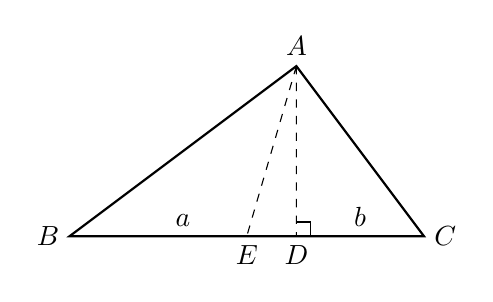
\begin{tikzpicture}[scale = 1.8]
        \draw [thick] (0,0) node [left] {$B$} -- (2.5,0) node [right] {$C$} -- (1.6,1.2) node [above] {$A$} -- cycle;
        \draw [dashed] (1.6,1.2) -- (1.6,0) node [below] {$D$} (1.6,1.2) -- (1.25,0) node [below] {$E$};
        \draw [thin] (1.7,0) -- (1.7,0.1) -- (1.6,0.1);
        \draw (0.8,0) node [above] {$a$} (2.05,0) node [above] {$b$};
    \end{tikzpicture}
\end{center}


关联目标:

K0118001B|D01003B|知道算术平均值和几何平均值的概念.

K0118002B|D01003B|经历平均值不等式的证明过程, 理解取等号的条件.

答案: 暂无答案

解答或提示: 暂无解答与提示

使用记录:

暂无使用记录


出处: 教材复习题
\item { (000032)}如图, 已知直角梯形$ABCD$的顶点$A(a, 0)$、$B(b, 0)$位于$x$轴上, 顶点$C$、$D$落在函数$y=|x|$的图像上, $M$、$N$分别为线段$AB$、$CD$的中点, $O$为坐标原点, $Q$为线段$OC$与线段$MN$的交点.\\
(1) 求中点$M$的坐标, 以及线段$MQ$、$MN$的长度;\\
(2) 用不等式表示$MQ$、$MN$长度的大小关系.
\begin{center}
    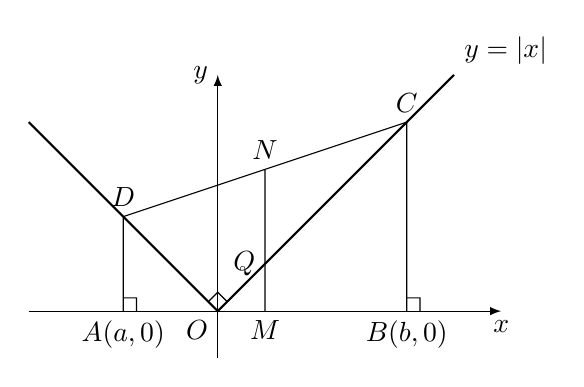
\begin{tikzpicture}[scale = 1.2,>=latex]
        \draw [->] (-2,0) -- (3,0) node [below] {$x$};
        \draw [->] (0,-0.5) -- (0,2.5) node [left] {$y$};
        \draw (0,0) node [below left] {$O$};
        \draw [thick] (-2,2) -- (0,0) -- (2.5,2.5) node [above right] {$y=|x|$};
        \draw [thin] (-0.1,0.1) -- (0,0.2) -- (0.1,0.1) (2.14,0) -- (2.14,0.14) -- (2,0.14) (-0.86,0) -- (-0.86,0.14) -- (-1,0.14);
        \draw (-1,0) node [below] {$A(a,0)$} -- (-1,1) node [above] {$D$} -- (0.5,1.5) node [above] {$N$} -- (2,2) node [above] {$C$} -- (2,0) node [below] {$B(b,0)$} (0.5,1.5) -- (0.5,0.5) node [left] {$Q$} -- (0.5,0) node [below] {$M$}; 
    \end{tikzpicture}
\end{center}


关联目标:

K0120001B|D01003B|经历三角不等式的证明过程, 理解取等号的条件.

答案: 暂无答案

解答或提示: 暂无解答与提示

使用记录:

暂无使用记录


出处: 教材复习题
\item { (000033)}已知一元二次方程$x^2+px+p=0$的两个实根分别为$\alpha$、$\beta$, 且$\alpha^2$+$\beta^2=3$, 求实数$p$的值.


关联目标:

K0109004B|D01004B|在给定二次方程的前提下, 能计算用根表示的简单二元对称多项式的值.

答案: 暂无答案

解答或提示: 暂无解答与提示

使用记录:

暂无使用记录


出处: 教材复习题
\item { (000034)}已知一元二次方程$2x^2-4x+m+3=0$有两个同号实根, 求实数$m$的取值范围.


关联目标:

K0109004B|D01004B|在给定二次方程的前提下, 能计算用根表示的简单二元对称多项式的值.

答案: 暂无答案

解答或提示: 暂无解答与提示

使用记录:

暂无使用记录


出处: 教材复习题
\item { (000035)}设$a,b\in \mathbf{R}$, 已知关于$x$的不等式$(a+b)x+(b-2a)<0$的解集为$(1, +\infty)$, 求不等式$(a-b)x+3b-a>0$的解集.


关联目标:

K0112001B|D01004B|会求解(含有参数的)一元一次不等式(组), 并能用集合表示一元一次不等式(组)的解集.

答案: 暂无答案

解答或提示: 暂无解答与提示

使用记录:

暂无使用记录


出处: 教材复习题
\item { (000036)}解下列不等式:\\
(1) $-2< \dfrac 1{2x+1}\le 3$;\\
(2) $2<|x+1|\le 3$.


关联目标:

K0116002B|D01004B|会用转化为整式不等式(组)解一些简单的分式不等式.

K0117001B|D01004B|会用绝对值的几何意义求解一些基本的含绝对值的不等式.

答案: 暂无答案

解答或提示: 暂无解答与提示

使用记录:

暂无使用记录


出处: 教材复习题
\item { (000037)}已知集合$A=\{x||x-a|<2\}$, $B=\{x|\dfrac{2x-1}{x+2}<1\}$, 且$A\subseteq B$. 求实数$a$的取值范围.


关联目标:

K0116002B|D01004B|会用转化为整式不等式(组)解一些简单的分式不等式.

K0117001B|D01004B|会用绝对值的几何意义求解一些基本的含绝对值的不等式.

K0103001B|D01001B|理解集合之间包含的概念, 能识别给定集合的子集.

答案: 暂无答案

解答或提示: 暂无解答与提示

使用记录:

暂无使用记录


出处: 教材复习题
\item { (000038)}证明: 若$x>-1$, 则$x+\dfrac 1{x+1}\ge 1$, 并指出等号成立的条件.


关联目标:

K0118003B|D01003B|能运用平均值不等式比较大小、证明一些简单的不等式.

答案: 暂无答案

解答或提示: 暂无解答与提示

使用记录:

暂无使用记录


出处: 教材复习题
\item { (000039)}设$a$、$b$为正数, 且$a+b=2$. 求$\dfrac 1a+\dfrac 1b$的最小值.


关联目标:

K0119001B|D01003B|会运用平均值不等式求解较简单的最大值和最小值问题.

答案: 暂无答案

解答或提示: 暂无解答与提示

使用记录:

暂无使用记录


出处: 教材复习题
\item { (000040)}已知$a$、$b$、$c$都是正数, 求证: $\dfrac{b+c}{a}+\dfrac{c+a}{b}+\dfrac{a+b}{c}\ge 6$.


关联目标:

K0118003B|D01003B|能运用平均值不等式比较大小、证明一些简单的不等式.

答案: 暂无答案

解答或提示: 暂无解答与提示

使用记录:

暂无使用记录


出处: 教材复习题
\item { (000041)}设实数$x$、$y$满足$|x+y|=1$, 求$xy$的最大值.


关联目标:

K0119001B|D01003B|会运用平均值不等式求解较简单的最大值和最小值问题.

答案: 暂无答案

解答或提示: 暂无解答与提示

使用记录:

暂无使用记录


出处: 教材复习题
\item { (000042)}已知$a$、$b$为实数, 求证:$|a|+|b| \le |a+b| +|a-b|$, 并指出等号成立的条件.


关联目标:

K0120002B|D01003B|会运用三角不等式证明一些简单的不等式.

答案: 暂无答案

解答或提示: 暂无解答与提示

使用记录:

暂无使用记录


出处: 教材复习题
\item { (000043)}已知$a$、$b$是实数,\\
(1) 求证: $a^2+ab+b^2\ge 0$, 并指出等号成立的条件;\\
(2) 求证: 如果$a>b$, 那么$a^3>b^3$.


关联目标:

K0111003B|D01003B|会用不等式的性质、作差法证明一些简单的不等式.

答案: 暂无答案

解答或提示: 暂无解答与提示

使用记录:

暂无使用记录


出处: 教材复习题
\item { (000044)}解下列不等式:\\
(1) $\dfrac{3x-11}{x^2-6x+9}\le 1$;\\
(2) $|3-2x| \ge |x+1|$.


关联目标:

K0116002B|D01004B|会用转化为整式不等式(组)解一些简单的分式不等式.

K0117001B|D01004B|会用绝对值的几何意义求解一些基本的含绝对值的不等式.

答案: 暂无答案

解答或提示: 暂无解答与提示

使用记录:

暂无使用记录


出处: 教材复习题
\item { (000045)}已知集合$A=\{x|x^2-2x-3>0\}$, $B=\{x|x^2+px+q\le 0\}$. 若$A\cup B=\mathbf{R}$, 且$A\cap B=[-2,-1)$, 求实数$p$及$q$的值.


关联目标:

K0104001B|D01001B|理解两个集合的交集的含义, 在具体数学情境中, 能求两个集合的交集.

K0104003B|D01001B|理解两个集合的并集的含义, 在具体数学情境中, 能求两个集合的并集.

K0115002B|D01004B|在已知解集的情形下, 会求解含参一元二次不等式系数所满足的关系或者系数值.

答案: 暂无答案

解答或提示: 暂无解答与提示

使用记录:

暂无使用记录


出处: 教材复习题
\item { (000046)}已知实数$0<a<b$, 求证: $a<\dfrac{2ab}{a+b}<\sqrt{ab}<\dfrac{a+b}{2}<\sqrt{\dfrac{a^2+b^2}{2}}<b$.


关联目标:

K0118003B|D01003B|能运用平均值不等式比较大小、证明一些简单的不等式.

答案: 暂无答案

解答或提示: 暂无解答与提示

使用记录:

暂无使用记录


出处: 教材复习题
\item { (000047)}方程$(x-1)(x-2)(x-3)=0$的三个根$1$、$2$、$3$将数轴划分为四个区间, 即$(-\infty, 1)$, $(1, 2)$, $(2, 3)$, $(3, +\infty)$. 试在这四个区间上分别考察$(x-1)(x-2)(x-3)$的
符号, 从而得出不等式$(x-1)(x-2)(x-3)>0$与$(x-1)(x-2)(x-3)<0$的解集.\\
一般地, 对$x_1$、$x_2$、$x_3\in \mathbf{R}$, 且$x_1\le x_2\le x_3$, 试分别求不等式$(x-x_1)(x-x_2)(x-x_3)>0$与$(x-x_1)(x-x_2)(x-x_3)<0$的解集(提示: $x_1$、$x_2$、$x_3$相互之间可能相等, 需要分情况讨论).


关联目标:

K0113001B|D01004B|会用因式分解后两部分符号的讨论求解一元二次不等式.

K0116001B|D01004B|结合分类讨论, 会用不等式(组)解一些简单的分式不等式.

答案: 暂无答案

解答或提示: 暂无解答与提示

使用记录:

暂无使用记录


出处: 教材复习题
\item { (000056)}设$\log_{0.2}a>0$, $\log_{0.2}b>0$, 且$\log_{0.2}a\cdot \log_{0.2}b=1$, 求$\log_{0.2}(ab)$的最小值.


关联目标:

K0205002B|D02001B|会运用对数的定义以及运算性质解决简单的求值、化简以及生活实际问题.

K0119001B|D01003B|会运用平均值不等式求解较简单的最大值和最小值问题.

答案: 暂无答案

解答或提示: 暂无解答与提示

使用记录:

暂无使用记录


出处: 教材复习题
\item { (000059)}甲、乙两人同时解关于$x$的方程: $\log_2x+b+c\log_x2=0$. 甲写错了常数$b$, 得两根
$\dfrac 14$及$\dfrac 18$; 乙写错了常数$c$, 得两根$\dfrac 12$及$64$. 求这个方程的真正根.


关联目标:

K0109004B|D01004B|在给定二次方程的前提下, 能计算用根表示的简单二元对称多项式的值.

K0206002B|D02001B|会运用对数的运算性质以及换底公式解决较复杂的求值、化简以及证明等相关问题.

答案: 暂无答案

解答或提示: 暂无解答与提示

使用记录:

暂无使用记录


出处: 教材复习题
\item { (000073)}已知集合$A=\{y|y=(\dfrac 12)^x,\  x\in [-2, 0)\}$, 用列举法表示集合$B=\{y|y=\log_3x,\  x\in A\text{且}y\in \mathbf{Z}\}$.


关联目标:

K0102001B|D01001B|能在具体情境中用列举法描述集合.

K0102002B|D01001B|能在具体情境中用描述法描述集合.

K0210005B|D02002B|会作出指数函数的大致图像, 能根据其图像特征叙述其函数性质.

K0213007B|D02002B|会作出对数函数的大致图像, 能根据其图像特征叙述函数性质.

答案: 暂无答案

解答或提示: 暂无解答与提示

使用记录:

暂无使用记录


出处: 教材复习题
\item { (000074)}$\log_23$是有理数吗? 请证明你的结论.


关联目标:

K0204004B|D02001B|会进行指数式与对数式的互化, 以及对数式的化简.

K0107003B|D01002B|了解反证法的思想以及表达方式, 能正确使用反证法证明一些简单的数学命题.

答案: 暂无答案

解答或提示: 暂无解答与提示

使用记录:

暂无使用记录


出处: 教材复习题
\item { (000082)}已知$k$是常数, 设$\alpha$、$\beta$是二次方程$x^2-2kx+k+20=0$的两个实根. 问: 当$k$为
何值时, $(\alpha+1)^2+(\beta+1)^2$取到最小值?


关联目标:

K0109004B|D01004B|在给定二次方程的前提下, 能计算用根表示的简单二元对称多项式的值.

答案: 暂无答案

解答或提示: 暂无解答与提示

使用记录:

暂无使用记录


出处: 教材复习题
\item { (000084)}若函数$y=(a^2+4a-5)x^2-4(a-1)x+3$的图像都在$x$轴上方(不含$x$轴), 求实数$a$的取值范围.


关联目标:

K0115001B|D01004B|能通过对判别式讨论的方法解决含参一元二次(可能是一元一次, 可能不含未知数)不等式的恒成立问题.

K0223003B|D02004B|会用函数的观点求解一元二次不等式.

答案: 暂无答案

解答或提示: 暂无解答与提示

使用记录:

暂无使用记录


出处: 教材复习题
\item { (000105)}选择题:\\
(1) 若$0<x<\dfrac\pi 4$, 且$\lg (\sin x+\cos x)=\dfrac12(3\lg 2-\lg 5)$, 则$\cos x-\sin x$的值为\bracket{20}.
\fourch{$\dfrac{\sqrt{6}}3$}{$\dfrac{\sqrt{3}}2$}{$\dfrac{\sqrt{10}}5$}{$\dfrac{\sqrt{5}}4$}
(2) 下列命题中, 真命题为\bracket{20}.
\onech{若点$P(a, 2a)$($a\ne 0$)为角$\alpha$的终边上一点, 则$\sin \alpha=\dfrac{2\sqrt 5}5$}
{同时满足$\sin \alpha=\dfrac 12$, $\cos \alpha=\dfrac{\sqrt3}2$的角$\alpha$有且只有一个}
{如果角$\alpha$满足$-3\pi <\alpha<-\dfrac 52\pi$, 那么角$\alpha$是第二象限的角}
{$\tan x=-\sqrt 3$的解集为$\{x|x=k\pi -\dfrac\pi 3, \  k\in \mathbf{Z}\}$}


关联目标:

K0305001B|D03001B|会用同角三角函数的基本关系式($\sin^2\alpha+\cos^2\alpha=1$; $\tan\alpha=\dfrac{\sin\alpha}{\cos\alpha}$; $\cot\alpha=\dfrac{\cos\alpha}{\sin\alpha}$; $\tan\alpha\cdot \cot\alpha=1$), 在熟悉的情境中, 解决一些三角恒等式的化简与证明问题.

K0303001B|D03001B|掌握任意角的用比值给出的正弦、余弦、正切、余切的定义.

K0303002B|D03001B|掌握不同象限的角的正弦、余弦、正切和余切的符号.

K0308002B|D03002B|能借助角的三角比的特殊值解简单的三角方程.

答案: 暂无答案

解答或提示: 暂无解答与提示

使用记录:

暂无使用记录


出处: 教材复习题
\item { (000163)}填空题:\\
(1) 设$z=11-60\mathrm{i}$, 则$\mathrm{Re}z=$\blank{50}; $\mathrm{Im}z=$\blank{50}; $|z|=$\blank{50}; $\overline{z}=$\blank{50}.\\
(2) 下列三个命题中, 真命题是\blank{50}.\\
\textcircled{1} 在复平面上, 表示实数的点都在实轴上, 表示虚数的点都在虚轴上;\\
\textcircled{2} 任何一个表示虚数的点一定在某一个象限内;\\
\textcircled{3} 复数的模表示该复数在复平面上所对应的点到原点的距离.


关联目标:

K0512002B|D05004B|掌握复数的实部和虚部的概念.

K0514004B|D05005B|会用复数模的性质计算具体复数的模.

K0512005B|D05004B|理解共轭复数的概念.

K0513003B|D05004B|理解复数与复平面上点的对应关系.

答案: 暂无答案

解答或提示: 暂无解答与提示

使用记录:

暂无使用记录


出处: 教材复习题
\item { (000178)}判断下列命题的真假, 并说明理由:\\
(1) 若直线$l$与平面$M$斜交, 则$M$内不存在与$l$垂直的直线;\\
(2) 若直线$l\perp\text{平面}M$, 则$M$内不存在与$l$不垂直的直线;\\
(3) 若直线$l$与平面$M$斜交, 则$M$内不存在与$l$平行的直线;\\
(4) 若直线$l\parallel\text{平面}M$, 则$M$内不存在与$l$不平行的直线.


关联目标:

K0610001B|D06003B|知道直线与平面斜交的相关概念, 会用图形语言表示.

K0609001B|D06003B|从现实情境中抽象、形成直线与平面垂直的概念, 并能用图形和符号语言表示.

答案: 暂无答案

解答或提示: 暂无解答与提示

使用记录:

暂无使用记录


出处: 教材复习题
\item { (000181)}已知直线$l\perp\text{平面}\alpha$, 直线$m\subset\text{平面}\beta$, 判断下列命题的真假, 并说明理由:\\
(1) 若$\alpha\parallel \beta$, 则$l\perp m$;\\
(2) 若$\alpha\perp \beta$, 则$l\parallel m$;\\
(3) 若$l\parallel m$, 则$\alpha\perp \beta$;\\
(4) 若$l\perp m$, 则$\alpha\parallel \beta$.


关联目标:

K0612004B|D06004B|能在具体的情形中运用两个平面平行的性质定理证明简单的相关问题(如两直线平行).

K0613005B|D06004B|了解平面与平面垂直的概念, 并能用图形及符号语言表示.

答案: 暂无答案

解答或提示: 暂无解答与提示

使用记录:

暂无使用记录


出处: 教材复习题
\item { (000184)}已知直线$a$、$b$和平面$\alpha$、$\beta$, 判断下列命题的真假, 并说明理由:\\
(1) 若$a\parallel \alpha$, $b\perp a$, 则$b\perp \alpha$;\\
(2) 若$a\parallel \alpha$, $\alpha\perp \beta$, 则$a\perp \beta$;\\
(3) 若$a\parallel b$, $b\subset\alpha$, 则$a\parallel \alpha$.


关联目标:

K0609001B|D06003B|从现实情境中抽象、形成直线与平面垂直的概念, 并能用图形和符号语言表示.

K0608004B|D06003B|能在具体的情境中用直线与平面平行的性质定理证明简单的相关问题(如借助平面交线作已知直线的平行线).

答案: 暂无答案

解答或提示: 暂无解答与提示

使用记录:

暂无使用记录


出处: 教材复习题
\item { (000196)}判断下列命题是否正确, 并说明理由:\\
(1) 以直角三角形的一直角边为轴旋转所形成的旋转体是圆锥;\\
(2) 以直角梯形的一腰为轴旋转所形成的旋转体是圆台;\\
(3) 圆柱、圆锥、圆台都有两个底面;\\
(4) 圆锥的侧面展开图为扇形, 这个扇形所在圆的半径等于圆锥底面圆的半径.


关联目标:

K0621005B|D06006B|了解旋转体的概念与相关概念(轴, 旋转面), 理解旋转体和多面体的区别.

K0615007B|D06006B|了解圆柱及相关概念(含轴, 底面, 侧面, 母线, 高), 能用数学语言刻画圆柱的形成过程.

K0618005B|D06006B|了解圆锥及相关概念(轴, 顶点, 底面, 侧面, 母线, 高), 能用数学语言刻画圆锥的形成过程.

K0618007B|D06006B|了解台体的概念及相关名称(圆台, 棱台, 正棱台), 知道台体的问题可以转换为锥体解决.

答案: 暂无答案

解答或提示: 暂无解答与提示

使用记录:

暂无使用记录


出处: 教材复习题
\item { (000267)}判断下列命题是否正确, 并说明理由:\\
(1) 到两坐标轴距离相等的点的轨迹方程为$y=x$;\\
(2) 若$\triangle ABC$的三个顶点的坐标分别为$A(1, 1)$、$B(3, 1)$、$C(1, 3)$, 则边$BC$上的中线所在直线的方程为$y=x$;\\
(3) 与两点$A(-1, 0)$、$B(1, 0)$的连线的夹角为$90^\circ$的动点的轨迹方程为$x^2+y^2=1$.


关联目标:

K0709002X|D07004X|能在简单的情境中, 判断曲线与方程是否对应.

K0721002X|D07008X|掌握求简单的轨迹方程的三个基本步骤(建立合适的坐标系, 根据曲线的特征推导方程, 验证以方程的解为坐标的点都在所求曲线上).

答案: 暂无答案

解答或提示: 暂无解答与提示

使用记录:

暂无使用记录


出处: 教材复习题
\item { (000326)}若``$a>b$'', 则``$a^3>b^3$''是\blank{50}命题(填: 真、假).


关联目标:

暂未关联目标

答案: 真

解答或提示: 暂无解答与提示

使用记录:

20211119	2022届高三1班	\fcolorbox[rgb]{0,0,0}{1.000,0.000,0}{1.000}


出处: 赋能练习
\item { (000346)}设集合$A=\{x||x-2|<1,x\in \mathbf{R}\}$, 集合$B=\mathbf{Z}$, 则$A\cap B=$\blank{50}.


关联目标:

暂未关联目标

答案: $\{2\}$

解答或提示: 暂无解答与提示

使用记录:

20211203	2022届高三1班	\fcolorbox[rgb]{0,0,0}{1.000,0.140,0}{0.930}


出处: 赋能练习
\item { (000355)}有以下命题:\\
\textcircled{1} 若函数$f(x)$既是奇函数又是偶函数, 则$f(x)$的值域为$\{0\}$; \\
\textcircled{2} 若函数$f(x)$是偶函数, 则$f(|x|)=f(x)$;\\
\textcircled{3} 若函数$f(x)$在其定义域内不是单调函数, 则$f(x)$不存在反函数;\\
\textcircled{4} 若函数$f(x)$存在反函数${{f}^{-1}}(x)$, 且${{f}^{-1}}(x)$与$f(x)$不完全相同, 则$f(x)$与${{f}^{-1}}(x)$图像的公共点必在直线$y=x$上; \\
其中真命题的序号是\blank{50}(写出所有真命题的序号).


关联目标:

暂未关联目标

答案: \textcircled{1}\textcircled{2}

解答或提示: 暂无解答与提示

使用记录:

20211203	2022届高三1班	\fcolorbox[rgb]{0,0,0}{1.000,0.790,0}{0.605}

20220622	2022届高三1班  	\fcolorbox[rgb]{0,0,0}{1.000,0.232,0}{0.884}


出处: 赋能练习
\item { (000356)}若集合$A=\{x|y^2=x,y\in \mathbf{R}\}$, $B=\{y|y=\sin x,x\in \mathbf{R}\}$, 则$A\cap B=$\blank{50}.


关联目标:

暂未关联目标

答案: $[0,1]$

解答或提示: 暂无解答与提示

使用记录:

20211210	2022届高三1班	\fcolorbox[rgb]{0,0,0}{1.000,0.182,0}{0.909}


出处: 赋能练习
\item { (000377)}设全集$U=\mathbf{R}$, 集合$A=\{-1,0,1,2,3\}$, $B=\{x|x\ge 2\}$, 则$A\cap {\complement_U}B=$\blank{50}.


关联目标:

暂未关联目标

答案: $\{-1,0,1\}$

解答或提示: 暂无解答与提示

使用记录:

20211223	2022届高三1班	\fcolorbox[rgb]{0,0,0}{1.000,0.000,0}{1.000}


出处: 赋能练习
\item { (000386)}设集合$M=\{x|x^2=x\}$, $N=\{x|\lg x\le 0\}$, 则$M\cap N=$\blank{50}.


关联目标:

暂未关联目标

答案: $\{1\}$

解答或提示: 暂无解答与提示

使用记录:

20211230	2022届高三1班	\fcolorbox[rgb]{0,0,0}{1.000,0.090,0}{0.955}


出处: 赋能练习
\item { (000397)}已知集合$A=\{x|\dfrac12\le {2^x}<16\}$, $B=\{x|y=\log _2(9-x^2)\}$, 则$A\cap B=$\blank{50}.


关联目标:

暂未关联目标

答案: $[-1,3)$

解答或提示: 暂无解答与提示

使用记录:

20211231	2022届高三1班	\fcolorbox[rgb]{0,0,0}{1.000,0.136,0}{0.932}


出处: 赋能练习
\item { (000401)}已知$f(x)=\sin\dfrac\pi 3x$, $A=\{1,2,3,4,5,6,7,8\}$, 现从集合$A$中任取两个不同元素$s$、$t$, 则使得$f(s)\cdot f(t)=0$发生的概率是\blank{50}.


关联目标:

暂未关联目标

答案: $\frac{13}{28}$

解答或提示: 暂无解答与提示

使用记录:

20211231	2022届高三1班	\fcolorbox[rgb]{0,0,0}{1.000,0.410,0}{0.795}


出处: 赋能练习
\item { (000413)}集合$\{x|\cos (\pi \cos x)=0,x\in [0,\pi]\}=$\blank{50}(用列举法表示).


关联目标:

暂未关联目标

答案: $\{\frac{\pi }3,\frac{2\pi }3\}$

解答或提示: 暂无解答与提示

使用记录:

20220105	2022届高三1班	\fcolorbox[rgb]{0,0,0}{1.000,0.256,0}{0.872}


出处: 赋能练习
\item { (000416)}已知$U=\mathbf{R}$, 集合$A=\{x|4-2x\ge x+1\}$, 则${\complement_U}A=$\blank{50}.


关联目标:

暂未关联目标

答案: $\{x|x>1\}$

解答或提示: 暂无解答与提示

使用记录:

20220106	2022届高三1班	\fcolorbox[rgb]{0,0,0}{1.000,0.000,0}{1.000}


出处: 赋能练习
\item { (000426)}已知集合$A=\{1,2,4,6,8\}$, $B=\{x|x=2k,k\in A\}$, 则$A\cap B=$\blank{50}.


关联目标:

暂未关联目标

答案: $\{2,4,8\}$

解答或提示: 暂无解答与提示

使用记录:

20220111	2022届高三1班	\fcolorbox[rgb]{0,0,0}{1.000,0.046,0}{0.977}


出处: 赋能练习
\item { (000446)}若集合$M=\{x|{x^2}-2x<0\}$, $N=\{x||x|>1\}$, 则$M\cap N=$\blank{50}.


关联目标:

暂未关联目标

答案: $(1,2)$

解答或提示: 暂无解答与提示

使用记录:

20220221	2022届高三1班	\fcolorbox[rgb]{0,0,0}{1.000,0.000,0}{1.000}


出处: 赋能练习
\item { (000456)}设集合$A=\{2,3,4,12\}$, $B=\{0,1,2,3\}$, 则$A\cap B=$\blank{50}.


关联目标:

暂未关联目标

答案: $\{2,3\}$

解答或提示: 暂无解答与提示

使用记录:

20220222	2022届高三1班	\fcolorbox[rgb]{0,0,0}{1.000,0.000,0}{1.000}


出处: 赋能练习
\item { (000466)}已知集合$A=\{1,2,5\}$, $B=\{2,a\}$. 若$A\cup B=\{1,2,3,5\}$, 则$a=$\blank{50}.


关联目标:

暂未关联目标

答案: $3$

解答或提示: 暂无解答与提示

使用记录:

20220223	2022届高三1班	\fcolorbox[rgb]{0,0,0}{1.000,0.000,0}{1.000}


出处: 赋能练习
\item { (000476)}已知全集$U=\mathbf{N}$, 集合$A=\{1,2,3,4\}$, 集合$B=\{3,4,5\}$, 则$(\complement_U A)\cap B=$\blank{50}.


关联目标:

暂未关联目标

答案: $\{5\}$

解答或提示: 暂无解答与提示

使用记录:

20220224	2022届高三1班	\fcolorbox[rgb]{0,0,0}{1.000,0.046,0}{0.977}


出处: 赋能练习
\item { (000496)}已知全集$U=\mathbf{R}$, 集合$A=\{x||x-1|>1\}$, $B=\{x|\dfrac{x-3}{x+1}<0\}$, 则$(\complement_U A)\cap B=$\blank{50}.


关联目标:

暂未关联目标

答案: $[0,2]$

解答或提示: 暂无解答与提示

使用记录:

20220228	2022届高三1班	\fcolorbox[rgb]{0,0,0}{1.000,0.142,0}{0.929}


出处: 赋能练习
\item { (000506)}若全集$U=\mathbf{R}$, 集合$A=\{x|x\le 0\text{或} x\ge 2\}$, 则$\complement_U A=$\blank{50}.


关联目标:

暂未关联目标

答案: $A=\{x|0<x<2\}$

解答或提示: 暂无解答与提示

使用记录:

20220302	2022届高三1班	\fcolorbox[rgb]{0,0,0}{1.000,0.000,0}{1.000}


出处: 赋能练习
\item { (000514)}数列$\{a_n\}$的通项公式是$a_n=2n-1\ (n\in \mathbf{N}^*)$, 数列$\{b_n\}$的通项公式是$b_n=3n \ (n\in \mathbf{N}^*)$, 令集合$A=\{a_1,a_2,\cdots,a_n,\cdots\}$, $B=\{b_1,b_2,\cdots,b_n,\cdots\}$, $n\in \mathbf{N}^*$. 将集合$A\cup B$中的所有元素按从小到大的顺序排列, 构成的数列记为$\{c_n\}$. 则数列$\{c_n\}$的前$28$项的和$S_{28}=$\blank{50}.


关联目标:

暂未关联目标

答案: $820$

解答或提示: 暂无解答与提示

使用记录:

20220302	2022届高三1班	\fcolorbox[rgb]{0,0,0}{1.000,0.372,0}{0.814}


出处: 赋能练习
\item { (000526)}集合$P=\{x|0 \le x<3, x\in \mathbf{Z}\}$, $M=\{x|x^2 \le 9\}$, 则$P\cap M=$\blank{50}.


关联目标:

暂未关联目标

答案: $\{ 0,1,2 \}$

解答或提示: 暂无解答与提示

使用记录:

20220304	2022届高三1班	\fcolorbox[rgb]{0,0,0}{1.000,0.364,0}{0.818}


出处: 赋能练习
\item { (000536)}设全集$U=\{ 1,2,3,4,5\}$, 若集合$A=\{3,4,5\}$, 则$\complement_U A=$\blank{50}.


关联目标:

暂未关联目标

答案: $\{1,2\}$

解答或提示: 暂无解答与提示

使用记录:

20220307	2022届高三1班	\fcolorbox[rgb]{0,0,0}{1.000,0.000,0}{1.000}


出处: 赋能练习
\item { (000547)}已知集合$A=\{x|0<x<3\}$, $B=\{x|x^2\ge 4\}$, 则$A\cap B=$\blank{50}.


关联目标:

暂未关联目标

答案: $[2,3)$

解答或提示: 暂无解答与提示

使用记录:

20220309	2022届高三1班	\fcolorbox[rgb]{0,0,0}{1.000,0.046,0}{0.977}


出处: 赋能练习
\item { (000556)}设全集$U=\mathbf{Z}$, 集合$M=\{1,2\}$, $P=\{-2,-1,0,1,2\}$, 则$P\cap \complement_U M$=\blank{50}.


关联目标:

暂未关联目标

答案: $\{-2,-1,0\}$

解答或提示: 暂无解答与提示

使用记录:

20220310	2022届高三1班	\fcolorbox[rgb]{0,0,0}{1.000,0.000,0}{1.000}


出处: 赋能练习
\item { (000576)}已知集合$A=\{1,2,m\}$, $B=\{3,4\}$.若$A\cap B=\{3\}$, 则实数$m=$\blank{50}.


关联目标:

暂未关联目标

答案: $-\frac 35$

解答或提示: 暂无解答与提示

使用记录:

20220316	2022届高三1班	\fcolorbox[rgb]{0,0,0}{1.000,0.046,0}{0.977}


出处: 赋能练习
\item { (000596)}设全集$U=\{1,2,3,4\}$, 集合$A=\{x|x^2-5x+4<0,x\in \mathbf{Z}\}$, 则$\complement_U A$=\blank{50}.


关联目标:

暂未关联目标

答案: $\{1,4\}$

解答或提示: 暂无解答与提示

使用记录:

20220323	2022届高三1班	\fcolorbox[rgb]{0,0,0}{1.000,0.140,0}{0.930}


出处: 赋能练习
\item { (000602)}若行列式$\begin{vmatrix} 1 & 2 & 4 \\ \cos \dfrac x2 & \sin \dfrac x2 & 0 \\ \sin \dfrac x2 & \cos \dfrac x2 & 8 \end{vmatrix}$中元素$4$的代数余子式的值为$\dfrac12$, 则实数$x$的取值集合为\blank{50}.


关联目标:

暂未关联目标

答案: $\{ x|x=2k\pi \pm \frac{\pi }3,\ k\in \mathbf{Z}\}$

解答或提示: 暂无解答与提示

使用记录:

20220323	2022届高三1班	\fcolorbox[rgb]{0,0,0}{1.000,0.046,0}{0.977}


出处: 赋能练习
\item { (000617)}已知集合$M=\{x||x+1|\le 1\},N=\{-1,0,1\},$则$M\cap N=$\blank{50}.


关联目标:

暂未关联目标

答案: $\{-1,0\}$

解答或提示: 暂无解答与提示

使用记录:

20220325	2022届高三1班	\fcolorbox[rgb]{0,0,0}{1.000,0.046,0}{0.977}


出处: 赋能练习
\item { (000627)}若全集$U=\mathbf{R}$, 集合$A=\{x|x\ge 1\}\cup\{x|x<0\}$, 则$\complement_U A=$\blank{50}.


关联目标:

暂未关联目标

答案: $[0,1)$

解答或提示: 暂无解答与提示

使用记录:

20220329	2022届高三1班	\fcolorbox[rgb]{0,0,0}{1.000,0.000,0}{1.000}


出处: 赋能练习
\item { (000636)}集合$A=\{1,2,3,4\}$, $B=\{x|(x-1)(x-5)<0\}$, 则$A\cap B=$\blank{50}.


关联目标:

暂未关联目标

答案: $\{2,3,4\}$

解答或提示: 暂无解答与提示

使用记录:

20220330	2022届高三1班	\fcolorbox[rgb]{0,0,0}{1.000,0.000,0}{1.000}


出处: 赋能练习
\item { (000656)}已知集合$A=\{x|\ln x>0 \}$, $B=\{x|2^x<3\}$, 则\blank{50}.


关联目标:

暂未关联目标

答案: $(1,\log_2 3)$

解答或提示: 暂无解答与提示

使用记录:

20220406	2022届高三1班	\fcolorbox[rgb]{0,0,0}{1.000,0.094,0}{0.953}


出处: 赋能练习
\item { (000666)}已知集合$A=\{x|\dfrac{x-2}{x+1}\ge 0\}$, 集合$B=\{y|0 \le y<4\}$, 则$A\cap B$=\blank{50}.


关联目标:

暂未关联目标

答案: $[2,4)$

解答或提示: 暂无解答与提示

使用记录:

20220408	2022届高三1班	\fcolorbox[rgb]{0,0,0}{1.000,0.094,0}{0.953}


出处: 赋能练习
\item { (000686)}已知集合$A=\{x|x>-1, \ x\in \mathbf{R}\}$, 集合$B=\{x|x<2, \ x\in \mathbf{R}\}$, 则$A\cap B=$\blank{50}.


关联目标:

暂未关联目标

答案: $(-1,2)$

解答或提示: 暂无解答与提示

使用记录:

20220419	2022届高三1班	\fcolorbox[rgb]{0,0,0}{1.000,0.000,0}{1.000}


出处: 赋能练习
\item { (000700)}集合$A=\{1,3,a^2\}$, 集合$B=\{a+1,a+2\}$. 若$B\cup A=A$, 则实数$a=$\blank{50}.


关联目标:

暂未关联目标

答案: $2$

解答或提示: 暂无解答与提示

使用记录:

20220420	2022届高三1班	\fcolorbox[rgb]{0,0,0}{1.000,0.046,0}{0.977}


出处: 赋能练习
\item { (000706)}设全集$U=\mathbf{R}$, 若集合$A=\{2\}$,$B=\{x|-1<x<2\}$, 则$A\cap (\complement_UB)=$\blank{50}.


关联目标:

暂未关联目标

答案: $\{2\}$

解答或提示: 暂无解答与提示

使用记录:

20220422	2022届高三1班	\fcolorbox[rgb]{0,0,0}{1.000,0.094,0}{0.953}


出处: 赋能练习
\item { (000716)}已知集合$U=\{-1,0,1,2,-3\}$, $A=\{-1,0,2\}$, 则$\complement_U A=$\blank{50}.


关联目标:

暂未关联目标

答案: $\{1,3\}$

解答或提示: 暂无解答与提示

使用记录:

20220424	2022届高三1班	\fcolorbox[rgb]{0,0,0}{1.000,0.000,0}{1.000}


出处: 赋能练习
\item { (000726)}集合$A=\{x|\dfrac x{x-2}<0\}$,$B=\{x|x\in \mathbf{Z}\}$, 则$A\cap B$等于\blank{50}.


关联目标:

暂未关联目标

答案: $\{1\}$

解答或提示: 暂无解答与提示

使用记录:

20220426	2022届高三1班	\fcolorbox[rgb]{0,0,0}{1.000,0.046,0}{0.977}


出处: 赋能练习
\item { (000736)}已知全集$U=\mathbf{R}$, 集合$A=\{x|x^2-2x-3>0\}$, 则$\complement_U A=$\blank{50}.


关联目标:

暂未关联目标

答案: $[-1,3]$

解答或提示: 暂无解答与提示

使用记录:

20220427	2022届高三1班	\fcolorbox[rgb]{0,0,0}{1.000,0.046,0}{0.977}


出处: 赋能练习
\item { (000751)}从集合$\{-1,1,2,3\}$随机取一个为$m$, 从集合$\{-2,-1,1,2\}$随机取一个为$n$, 则方程$\dfrac{x^2}m+\dfrac{y^2}n=1$表示双曲线的概率为\blank{50}.


关联目标:

暂未关联目标

答案: $\frac 12$

解答或提示: 暂无解答与提示

使用记录:

20220429	2022届高三1班	\fcolorbox[rgb]{0,0,0}{1.000,0.326,0}{0.837}


出处: 赋能练习
\item { (000756)}已知集合$A=\{1,2,3\}B=\{1,m\}$, 若$3-m\in A$, 则非零实数$m$的数值是\blank{50}.


关联目标:

暂未关联目标

答案: $2$

解答或提示: 暂无解答与提示

使用记录:

20220506	2022届高三1班	\fcolorbox[rgb]{0,0,0}{1.000,0.280,0}{0.860}


出处: 赋能练习
\item { (000768)}已知集合$P=\{x|(x+1)(x-3)<0\}$, $Q=\{x||x|>2\}$, 则$P\cap Q$=\blank{50}.


关联目标:

暂未关联目标

答案: $\{x|2<x<3\}$

解答或提示: 暂无解答与提示

使用记录:

20220507	2022届高三1班	\fcolorbox[rgb]{0,0,0}{1.000,0.000,0}{1.000}


出处: 赋能练习
\item { (000775)}平面上三条直线$x-2y+1=0$, $x-1=0$, $x+ky=0$, 如果这三条直线将平面划分为六个部分, 则实数$k$的取值组成的集合$A=$\blank{50}.


关联目标:

暂未关联目标

答案: $\{–1, 0, –2\}$

解答或提示: 暂无解答与提示

使用记录:

20220507	2022届高三1班	\fcolorbox[rgb]{0,0,0}{1.000,0.838,0}{0.581}

20220622	2022届高三1班  	\fcolorbox[rgb]{0,0,0}{1.000,0.186,0}{0.907}


出处: 赋能练习
\item { (000776)}已知集合$A=\{1,3,5,7,9\}$, $B=\{0,1,2,3,4,5\}$, 则图中阴影部分集合用列举法表示的结果是\blank{50}.
\begin{center}
    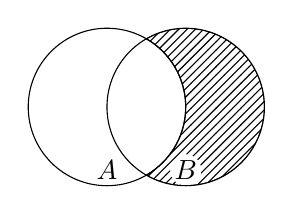
\begin{tikzpicture}
        \begin{scope}[even odd rule]
            \clip  (1,-0.8) circle (0.2) (1,0) circle (1);
            \filldraw [pattern = {north east lines}] (0.5,{0.5*sqrt(3)}) arc (60:-60:1) arc (-120:120:1);
        \end{scope}
        \draw (0,0) circle (1);
        \draw (1,0) circle (1);
        \draw (0,-0.8) node {$A$};
        \draw (1,-0.8) node {$B$};
    \end{tikzpicture}
\end{center}


关联目标:

暂未关联目标

答案: $\{0, 2, 4\}$

解答或提示: 暂无解答与提示

使用记录:

20220510	2022届高三1班	\fcolorbox[rgb]{0,0,0}{1.000,0.000,0}{1.000}


出处: 赋能练习
\item { (000836)}已知集合$A=\{1,2,m\}$,$B=\{2,4\}$, 若$A\cup B=\{1,2,3,4\}$, 则实数$m=$\blank{50}.


关联目标:

暂未关联目标

答案: $3$

解答或提示: 暂无解答与提示

使用记录:

20220525	2022届高三1班	\fcolorbox[rgb]{0,0,0}{1.000,0.000,0}{1.000}


出处: 赋能练习
\item { (000846)}已知全集$U=\mathbf{R}$,若集合$A=\{x|\dfrac x{x-1}>0\}$, 则$\complement_U A=$\blank{50}.


关联目标:

暂未关联目标

答案: $[0,1]$

解答或提示: 暂无解答与提示

使用记录:

20220526	2022届高三1班	\fcolorbox[rgb]{0,0,0}{1.000,0.046,0}{0.977}


出处: 赋能练习
\item { (000857)}设集合$A=\{x||x|<2,\ x\in \mathbf{R}\}$, $B=\{x|x^2-4x+3\ge 0, \ x\in \mathbf{R}\}$, 则$A\cap B=$\blank{50}.


关联目标:

暂未关联目标

答案: $(-2,1]$

解答或提示: 暂无解答与提示

使用记录:

20220527	2022届高三1班	\fcolorbox[rgb]{0,0,0}{1.000,0.094,0}{0.953}


出处: 赋能练习
\item { (000879)}若集合$A=\{x|3x+1>0\}$, $B=\{x||x-1|<2\}$, 则$A\cap B$=\blank{50}.


关联目标:

暂未关联目标

答案: $(-\frac 13,3)$

解答或提示: 暂无解答与提示

使用记录:

20220602	2022届高三1班	\fcolorbox[rgb]{0,0,0}{1.000,0.094,0}{0.953}


出处: 赋能练习
\item { (000889)}从集合$A=\{1,2,3,4,5,6,7,8,9,10\}$中任取两个数, 欲使取到的一个数大于$k$, 另一个数小于$k$(其中$k\in A$)的概率是$\dfrac25$, 则$k=$\blank{50}.


关联目标:

暂未关联目标

答案: $4$或$7$

解答或提示: 暂无解答与提示

使用记录:

20220602	2022届高三1班	\fcolorbox[rgb]{0,0,0}{1.000,0.280,0}{0.860}


出处: 赋能练习
\item { (000891)}已知集合$A=\{x||x-2|<a\}$, $B=\{x|x^2-2x-3<0\}$, 若$B\subseteq A$, 则实数$a$的取值范围是\blank{50}.


关联目标:

暂未关联目标

答案: $a\ge 3$

解答或提示: 暂无解答与提示

使用记录:

20220607	2022届高三1班	\fcolorbox[rgb]{0,0,0}{1.000,0.372,0}{0.814}


出处: 赋能练习
\item { (000899)}设集合$M=\{x|x^2=x\}$, $N=\{x|\log_2 x\le 0\}$, 则$M\cup N=$\blank{50}.


关联目标:

暂未关联目标

答案: $[0,1]$

解答或提示: 暂无解答与提示

使用记录:

20220613	2022届高三1班	\fcolorbox[rgb]{0,0,0}{1.000,0.418,0}{0.791}


出处: 赋能练习
\item { (000905)}若行列式$\begin{vmatrix}   1 & 2 & 4 \\   \cos (\pi +x) & 2 & 0 \\   -1 & 1 & 6 \end{vmatrix}$中的元素$4$的代数余子式的值等于$\dfrac32$, 则实数$x$的取值集合为\blank{50}.


关联目标:

暂未关联目标

答案: $\{x|x=2k\pi\pm\frac{\pi}3, \ k\in \mathbf{Z}\}$

解答或提示: 暂无解答与提示

使用记录:

20220613	2022届高三1班	\fcolorbox[rgb]{0,0,0}{1.000,0.326,0}{0.837}


出处: 赋能练习
\item { (000910)}若集合$A=\{x|y=\sqrt{x-1},\ x\in \mathbf{R}\}$, $B=\{x||x|\le 1,\ x\in \mathbf{R}\}$, 则$A\cap B=$\blank{50}.


关联目标:

暂未关联目标

答案: $\{1\}$

解答或提示: 暂无解答与提示

使用记录:

20220615	2022届高三1班	\fcolorbox[rgb]{0,0,0}{1.000,0.046,0}{0.977}


出处: 赋能练习
\item { (000932)}集合$A=\{x|x^2-3x<0\}$, $B=\{x||x|<2\}$, 则$A\cup B$等于\blank{50}.


关联目标:

暂未关联目标

答案: $(-2,3)$

解答或提示: 暂无解答与提示

使用记录:

20220622	2022届高三1班	\fcolorbox[rgb]{0,0,0}{1.000,0.094,0}{0.953}


出处: 赋能练习
\item { (000942)}已知集合$A=\{-1,3,2m-1\}$, 集合$B=\{3,m^2\}$. 若$B\subseteq A$, 则实数$m=$\blank{50}.


关联目标:

暂未关联目标

答案: $1$

解答或提示: 暂无解答与提示

使用记录:

20220624	2022届高三1班	\fcolorbox[rgb]{0,0,0}{1.000,0.000,0}{1.000}


出处: 赋能练习
\item { (000962)}已知$x\ge 1$, $y\ge 0$, 集合$A=\{(x,y)|x+y\le 4\}$, $B=\{(x,y)|x-y+t=0\}$. 如果$A\cap B\ne \varnothing$,则$t$的取值范围是\blank{50}.


关联目标:

暂未关联目标

答案: $[-4,2]$

解答或提示: 暂无解答与提示

使用记录:

20220628	2022届高三1班	\fcolorbox[rgb]{0,0,0}{1.000,0.094,0}{0.953}


出处: 赋能练习
\item { (000964)}已知全集$U=\mathbf{R}$, 集合$A=\{x|(x-1)(x-4)\le 0\}$, 则集合$A$的补集$\complement_UA=$\blank{50}.


关联目标:

暂未关联目标

答案: $(-\infty ,1)\cup (4,+\infty)$

解答或提示: 暂无解答与提示

使用记录:

20220629    2022届高三1班  	\fcolorbox[rgb]{0,0,0}{1.000,0.046,0}{0.977}


出处: 赋能练习
\item { (000975)}下列各句是否是命题? (T or F)\\ 
\blank{30} (1) $1$是偶数;\\ 
\blank{30} (2) 线段$AB$太长;\\ 
\blank{30} (3) 所有有理数都大于零;\\ 
\blank{30} (4) $2>5$;\\ 
\blank{30} (5) 存在实数$a$使$|a|=-a$不成立.


关联目标:

暂未关联目标

答案: 暂无答案

解答或提示: 暂无解答与提示

使用记录:

2016届11班	\fcolorbox[rgb]{0,0,0}{1.000,0.000,0}{1.000}	\fcolorbox[rgb]{0,0,0}{1.000,0.000,0}{1.000}	\fcolorbox[rgb]{0,0,0}{1.000,0.000,0}{1.000}	\fcolorbox[rgb]{0,0,0}{1.000,0.000,0}{1.000}	\fcolorbox[rgb]{0,0,0}{1.000,0.000,0}{1.000}

2016届12班	\fcolorbox[rgb]{0,0,0}{1.000,0.154,0}{0.923}	\fcolorbox[rgb]{0,0,0}{1.000,0.000,0}{1.000}	\fcolorbox[rgb]{0,0,0}{1.000,0.154,0}{0.923}	\fcolorbox[rgb]{0,0,0}{1.000,0.256,0}{0.872}	\fcolorbox[rgb]{0,0,0}{1.000,0.000,0}{1.000}


出处: 2016届创新班作业	1101-命题及其运算
\item { (000976)}在下列各命题的右边写出其否定形式(否定命题).\\ 
(1) $2 \times 2 =5$; \blank{150}.\\ 
(2) $\sqrt{3-\pi}$有意义; \blank{150}.\\ 
(3) $a$不是非负数; \blank{150}.\\ 
(4) $\sqrt{a}$不是无理数; \blank{150}.(本小题中已知$a\ge 0$)\\ 
(5) $x=1$不是方程$x(x+1)=0$的根; \blank{150}.


关联目标:

暂未关联目标

答案: 暂无答案

解答或提示: 暂无解答与提示

使用记录:

2016届11班	\fcolorbox[rgb]{0,0,0}{1.000,0.000,0}{1.000}	\fcolorbox[rgb]{0,0,0}{1.000,0.052,0}{0.974}	\fcolorbox[rgb]{0,0,0}{1.000,0.462,0}{0.769}	\fcolorbox[rgb]{0,0,0}{1.000,0.462,0}{0.769}	\fcolorbox[rgb]{0,0,0}{1.000,0.206,0}{0.897}

2016届12班	\fcolorbox[rgb]{0,0,0}{1.000,0.102,0}{0.949}	\fcolorbox[rgb]{0,0,0}{1.000,0.052,0}{0.974}	\fcolorbox[rgb]{0,0,0}{1.000,0.358,0}{0.821}	\fcolorbox[rgb]{0,0,0}{1.000,0.358,0}{0.821}	\fcolorbox[rgb]{0,0,0}{1.000,0.256,0}{0.872}


出处: 2016届创新班作业	1101-命题及其运算
\item { (000977)}下列各组命题是否互为否定形式(否定命题)? (T or F).\\ 
\blank{30}(1) 所有直角三角形都不是等边三角形; / 所有直角三角形都是等边三角形.\\ 
\blank{30}(2) 对一切实数$x$, $x^2+1 \ne 0$; / 存在实数$x$, 使得$x^2+1=0$.\\ 
\blank{30}(3) 所有一元二次方程都没有实数根; / 有些一元二次方程没有实数根.\\ 
\blank{30}(4) 所有自然数都不是$0$; / 所有自然数都是$0$.\\ 
\blank{30}(5) 存在实数$x$, 使得$x^2-5x+6=0$; / 所有实数$x$, 都使得$x^2-5x+6\ne 0$.\\ 
\blank{30}(6) 对于一些实数$x$, $x^3+1=0$; / 对于一些实数$x$, $x^3+1\ne 0$.\\ 
\blank{30}(7) 有些三角形两边的平方和等于第三边的平方; / 所有三角形两边的平方和不等于第三边的平方.\\ 
\blank{30}(8) 对于某些实数$x$, $x=x+1$; / 对于任意实数$x$, $x \ne x+1$.\\ 
\blank{30}(9) 负实数没有平方根; / 负实数有平方根.


关联目标:

暂未关联目标

答案: 暂无答案

解答或提示: 暂无解答与提示

使用记录:

2016届11班	\fcolorbox[rgb]{0,0,0}{1.000,0.102,0}{0.949}	\fcolorbox[rgb]{0,0,0}{1.000,0.000,0}{1.000}	\fcolorbox[rgb]{0,0,0}{1.000,0.052,0}{0.974}	\fcolorbox[rgb]{0,0,0}{1.000,0.102,0}{0.949}	\fcolorbox[rgb]{0,0,0}{1.000,0.206,0}{0.897}	\fcolorbox[rgb]{0,0,0}{1.000,0.000,0}{1.000}	\fcolorbox[rgb]{0,0,0}{1.000,0.000,0}{1.000}	\fcolorbox[rgb]{0,0,0}{1.000,0.000,0}{1.000}	\fcolorbox[rgb]{0,0,0}{1.000,0.256,0}{0.872}

2016届12班	\fcolorbox[rgb]{0,0,0}{1.000,0.000,0}{1.000}	\fcolorbox[rgb]{0,0,0}{1.000,0.052,0}{0.974}	\fcolorbox[rgb]{0,0,0}{1.000,0.052,0}{0.974}	\fcolorbox[rgb]{0,0,0}{1.000,0.000,0}{1.000}	\fcolorbox[rgb]{0,0,0}{1.000,0.052,0}{0.974}	\fcolorbox[rgb]{0,0,0}{1.000,0.000,0}{1.000}	\fcolorbox[rgb]{0,0,0}{1.000,0.000,0}{1.000}	\fcolorbox[rgb]{0,0,0}{1.000,0.102,0}{0.949}	\fcolorbox[rgb]{0,0,0}{1.000,0.206,0}{0.897}


出处: 2016届创新班作业	1101-命题及其运算
\item { (000978)}在下列各命题的右边写出其否定命题.\\ 
(1) $a=0$且$b=0$; \blank{150}.\\ 
(2) $x>0$或$x \le -3$; \blank{150}.\\ 
(3*) 平面上的点$P$在第一象限或第二象限; \blank{150}.


关联目标:

暂未关联目标

答案: 暂无答案

解答或提示: 暂无解答与提示

使用记录:

2016届11班	\fcolorbox[rgb]{0,0,0}{1.000,0.052,0}{0.974}	\fcolorbox[rgb]{0,0,0}{1.000,0.206,0}{0.897}	\fcolorbox[rgb]{0,0,0}{0.924,1.000,0}{0.462}

2016届12班	\fcolorbox[rgb]{0,0,0}{1.000,0.154,0}{0.923}	\fcolorbox[rgb]{0,0,0}{1.000,0.206,0}{0.897}	\fcolorbox[rgb]{0,0,0}{0.872,1.000,0}{0.436}


出处: 2016届创新班作业	1101-命题及其运算
\item { (000979)}下列各组命题是否互为否定形式(否定命题)? (T or F).\\ 
\blank{30}(1) $a,b$都是偶数; / $a,b$都不是偶数.\\ 
\blank{30}(2) $a,b$不都是偶数; / $a,b$都是偶数.\\ 
\blank{30}(3) $a,b$中至少有一个是偶数; / $a,b$中至多有两个是偶数.\\ 
\blank{30}(4) $a,b$都不是偶数; / $a,b$都是奇数.


关联目标:

暂未关联目标

答案: 暂无答案

解答或提示: 暂无解答与提示

使用记录:

2016届11班	\fcolorbox[rgb]{0,0,0}{1.000,0.102,0}{0.949}	\fcolorbox[rgb]{0,0,0}{1.000,0.154,0}{0.923}	\fcolorbox[rgb]{0,0,0}{1.000,0.000,0}{1.000}	\fcolorbox[rgb]{0,0,0}{1.000,0.000,0}{1.000}

2016届12班	\fcolorbox[rgb]{0,0,0}{1.000,0.052,0}{0.974}	\fcolorbox[rgb]{0,0,0}{1.000,0.102,0}{0.949}	\fcolorbox[rgb]{0,0,0}{1.000,0.052,0}{0.974}	\fcolorbox[rgb]{0,0,0}{1.000,0.000,0}{1.000}


出处: 2016届创新班作业	1101-命题及其运算
\item { (000981)}在下列各命题的右边写出其否定形式.\\ 
(1) 若$x$是实数, 则$x^2+x+1>0$; \blank{30}$x$是实数, 使得$x^2+x+1$\blank{10}$0$.\\ 
(2) 若$a>0$, 则$|a|\le a$; \blank{150}.\\ 
(3) 若实数$x$满足$x^2-x=0$, 则$x=1$或$x=0$; \blank{150}.\\ 
(4) 若实数$x$满足$x^2-x<0$, 则$0<x<1$; \blank{150}.


关联目标:

暂未关联目标

答案: 暂无答案

解答或提示: 暂无解答与提示

使用记录:

2016届11班	\fcolorbox[rgb]{0,0,0}{1.000,0.564,0}{0.718}	\fcolorbox[rgb]{0,0,0}{1.000,0.256,0}{0.872}	\fcolorbox[rgb]{0,0,0}{1.000,0.308,0}{0.846}	\fcolorbox[rgb]{0,0,0}{1.000,0.718,0}{0.641}

2016届12班	\fcolorbox[rgb]{0,0,0}{1.000,0.052,0}{0.974}	\fcolorbox[rgb]{0,0,0}{0.924,1.000,0}{0.462}	\fcolorbox[rgb]{0,0,0}{1.000,0.924,0}{0.538}	\fcolorbox[rgb]{0,0,0}{0.872,1.000,0}{0.436}


出处: 2016届创新班作业	1101-命题及其运算
\item { (000983)}用反证法证明如下命题:\\ 
(1) 已知$n$是整数. 如果$3$整除$n^3$, 则$3$整除$n$(提示: 讨论$n=3k,3k+1,3k+2$, 其中$k$是整数);\\ 
(2) 如果实数$x$满足$x^{101}-4x^2+8x-1=0$, 则$x>0$;\\ 
(3) $\sqrt[3]{3}$是无理数(提示: 可借鉴讲义上$\sqrt{6}$是无理数的证明方法);\\ 
(4*) $\sqrt{2}+\sqrt{3}$是无理数.


关联目标:

暂未关联目标

答案: 暂无答案

解答或提示: 暂无解答与提示

使用记录:

2016届11班	\fcolorbox[rgb]{0,0,0}{1.000,0.924,0}{0.538}	\fcolorbox[rgb]{0,0,0}{1.000,0.358,0}{0.821}	\fcolorbox[rgb]{0,0,0}{1.000,0.666,0}{0.667}	\fcolorbox[rgb]{0,0,0}{1.000,0.410,0}{0.795}

2016届12班	\fcolorbox[rgb]{0,0,0}{1.000,0.666,0}{0.667}	\fcolorbox[rgb]{0,0,0}{1.000,0.154,0}{0.923}	\fcolorbox[rgb]{0,0,0}{1.000,0.924,0}{0.538}	\fcolorbox[rgb]{0,0,0}{1.000,0.358,0}{0.821}


出处: 2016届创新班作业	1102-反证法
\item { (000985)}写出下列各命题的逆命题, 否命题, 逆否命题, 并判断真假.\\ 
(1) (已知$a,b$均为实数) 若$a^2+b^2=0$, 则$a=0$. 原命题的真值: \blank{30};\\ 
逆命题: \blank{250}; 逆命题的真值: \blank{30};\\ 
否命题: \blank{250}; 否命题的真值: \blank{30};\\ 
逆否命题: \blank{250}; 逆否命题的真值: \blank{30}.\\ 
(2) 若$ab=0$, 则$a=0$或$b=0$. 原命题的真值: \blank{30};\\ 
逆命题: \blank{250}; 逆命题的真值: \blank{30};\\ 
否命题: \blank{250}; 否命题的真值: \blank{30};\\ 
逆否命题: \blank{250}; 逆否命题的真值: \blank{30}.\\ 
(3) (已知$a,b$均为整数) 若$a,b$都是偶数, 则$a+b$是偶数. 原命题的真值: \blank{30};\\ 
逆命题: \blank{250}; 逆命题的真值: \blank{30};\\ 
否命题: \blank{250}; 否命题的真值: \blank{30};\\ 
逆否命题: \blank{250}; 逆否命题的真值: \blank{30}.\\ 
(4) (已知$a,b$均为整数) 若$ab$是奇数, 则$a,b$中至少有一个是奇数. 原命题的真值: \blank{30};\\ 
逆命题: \blank{250}; 逆命题的真值: \blank{30};\\ 
否命题: \blank{250}; 否命题的真值: \blank{30};\\ 
逆否命题: \blank{250}; 逆否命题的真值: \blank{30}.


关联目标:

暂未关联目标

答案: 暂无答案

解答或提示: 暂无解答与提示

使用记录:

2016届11班	\fcolorbox[rgb]{0,0,0}{1.000,0.052,0}{0.974}	\fcolorbox[rgb]{0,0,0}{1.000,0.256,0}{0.872}	\fcolorbox[rgb]{0,0,0}{1.000,0.308,0}{0.846}	\fcolorbox[rgb]{0,0,0}{1.000,0.256,0}{0.872}

2016届12班	\fcolorbox[rgb]{0,0,0}{1.000,0.052,0}{0.974}	\fcolorbox[rgb]{0,0,0}{1.000,0.154,0}{0.923}	\fcolorbox[rgb]{0,0,0}{1.000,0.308,0}{0.846}	\fcolorbox[rgb]{0,0,0}{1.000,0.462,0}{0.769}


出处: 2016届创新班作业	1103-假言命题的四种形式及充分必要条件
\item { (000989)}判断下列各组对象是否组成集合. (T or F)\\ 
\blank{30} (1) 大于$0$的偶数全体.\\ 
\blank{30} (2) 绝对值小于$0$的实数全体.\\ 
\blank{30} (3) 很小的数的全体.


关联目标:

暂未关联目标

答案: 暂无答案

解答或提示: 暂无解答与提示

使用记录:

2016届11班	\fcolorbox[rgb]{0,0,0}{1.000,0.000,0}{1.000}	\fcolorbox[rgb]{0,0,0}{1.000,0.256,0}{0.872}	\fcolorbox[rgb]{0,0,0}{1.000,0.000,0}{1.000}

2016届12班	\fcolorbox[rgb]{0,0,0}{1.000,0.000,0}{1.000}	\fcolorbox[rgb]{0,0,0}{1.000,0.000,0}{1.000}	\fcolorbox[rgb]{0,0,0}{1.000,0.000,0}{1.000}


出处: 2016届创新班作业	1104-集合及其表示
\item { (000990)}用描述法或列举法(自行择其一种)表示下列集合.\\ 
(1) 大于$0$且小于$3$的实数的全体.\\ 
(2) 方程$x^3-x=0$的解的全体.\\ 
(3) 一次函数$y=2x+1$图像上所有点的全体.\\ 
(4) 被$3$除余$2$的整数的全体.


关联目标:

暂未关联目标

答案: 暂无答案

解答或提示: 暂无解答与提示

使用记录:

2016届11班	\fcolorbox[rgb]{0,0,0}{1.000,0.102,0}{0.949}	\fcolorbox[rgb]{0,0,0}{1.000,0.102,0}{0.949}	\fcolorbox[rgb]{0,0,0}{1.000,0.000,0}{1.000}	\fcolorbox[rgb]{0,0,0}{1.000,0.462,0}{0.769}

2016届12班	\fcolorbox[rgb]{0,0,0}{1.000,0.052,0}{0.974}	\fcolorbox[rgb]{0,0,0}{1.000,0.154,0}{0.923}	\fcolorbox[rgb]{0,0,0}{1.000,0.052,0}{0.974}	\fcolorbox[rgb]{0,0,0}{1.000,0.564,0}{0.718}


出处: 2016届创新班作业	1104-集合及其表示
\item { (000991)}用列举法表示下列集合:\\ 
(1) $\left\{x\left| \dfrac{6}{3-x}\in\mathbf{Z},x\in\mathbf{Z}\right.\right\}$;\\ 
(2) $\{(x,y)|x+y=4,x,y\in\mathbf{N}\}$.


关联目标:

暂未关联目标

答案: 暂无答案

解答或提示: 暂无解答与提示

使用记录:

2016届11班	\fcolorbox[rgb]{0,0,0}{1.000,0.512,0}{0.744}	\fcolorbox[rgb]{0,0,0}{1.000,0.000,0}{1.000}

2016届12班	\fcolorbox[rgb]{0,0,0}{1.000,0.564,0}{0.718}	\fcolorbox[rgb]{0,0,0}{1.000,0.102,0}{0.949}


出处: 2016届创新班作业	1104-集合及其表示
\item { (000992)}在直角坐标系中, 用图形表示下列集合:\\ 
(1) $\{(x,y)|\ 2<x<6,1<y<4,x,y\in\mathbf{R}\}$; \hfill (2) $\{(x,y)|\ 2<x<6,1<y<4,x,y\in\mathbf{Z}\}$.


关联目标:

暂未关联目标

答案: 暂无答案

解答或提示: 暂无解答与提示

使用记录:

2016届11班	\fcolorbox[rgb]{0,0,0}{0.770,1.000,0}{0.385}	\fcolorbox[rgb]{0,0,0}{1.000,0.564,0}{0.718}

2016届12班	\fcolorbox[rgb]{0,0,0}{0.512,1.000,0}{0.256}	\fcolorbox[rgb]{0,0,0}{1.000,0.358,0}{0.821}


出处: 2016届创新班作业	1104-集合及其表示
\item { (000993)}集合$\left\{a,\dfrac{b}{a},1\right\}$和$\{0,a+b,a^2\}$ 表示同一个集合, 求实数$a,b$的值.


关联目标:

暂未关联目标

答案: 暂无答案

解答或提示: 暂无解答与提示

使用记录:

2016届11班	\fcolorbox[rgb]{0,0,0}{1.000,0.358,0}{0.821}

2016届12班	\fcolorbox[rgb]{0,0,0}{1.000,0.564,0}{0.718}


出处: 2016届创新班作业	1104-集合及其表示
\item { (000994)}已知$a$是实数, 集合$M=\{x|\ ax^2+2x+a=0\}$有且仅有一个元素. 求满足上述条件的$a$所构成的集合.


关联目标:

暂未关联目标

答案: 暂无答案

解答或提示: 暂无解答与提示

使用记录:

2016届11班	\fcolorbox[rgb]{0,0,0}{1.000,0.616,0}{0.692}

2016届12班	\fcolorbox[rgb]{0,0,0}{1.000,0.616,0}{0.692}


出处: 2016届创新班作业	1104-集合及其表示
\item { (000995)}已知非空集合$M$中的元素都是正整数, 且满足性质: 若$x\in M$, 则$4-x\in M$. 求满足条件的集合$M$.


关联目标:

暂未关联目标

答案: 暂无答案

解答或提示: 暂无解答与提示

使用记录:

2016届11班	\fcolorbox[rgb]{0,0,0}{0.000,1.000,0}{0.000}

2016届12班	\fcolorbox[rgb]{0,0,0}{0.000,1.000,0}{0.000}


出处: 2016届创新班作业	1104-集合及其表示
\item { (000996)}以下各命题中, 真命题有: \blank{80}(可能多选).
\fourch{$\varnothing \in \varnothing$}{$\varnothing \in \{\varnothing\}$}{$\varnothing \subseteq \varnothing$}{$\varnothing \subseteq \{\varnothing\}$}


关联目标:

暂未关联目标

答案: 暂无答案

解答或提示: 暂无解答与提示

使用记录:

2016届11班	\fcolorbox[rgb]{0,0,0}{1.000,0.102,0}{0.949}

2016届12班	\fcolorbox[rgb]{0,0,0}{1.000,0.474,0}{0.763}


出处: 2016届创新班作业	1105-集合的关系
\item { (000997)}以下各命题中, 真命题有: \blank{80}(可能多选).
\fourch{$5\in \{x|x\le 10\}$}{$\{5\} \in \{x|x\le 10\}$}{$\varnothing \in \{1,2,3,4\}$}{$\varnothing \subseteq \{1,2,3,4\}$}


关联目标:

暂未关联目标

答案: 暂无答案

解答或提示: 暂无解答与提示

使用记录:

2016届11班	\fcolorbox[rgb]{0,0,0}{1.000,0.358,0}{0.821}

2016届12班	\fcolorbox[rgb]{0,0,0}{1.000,0.264,0}{0.868}


出处: 2016届创新班作业	1105-集合的关系
\item { (000998)}满足$\{a_1,a_2\}\subseteq A\subsetneqq\{a_1,a_2,a_3,a_4,a_5,a_6\}$的集合$A$的个数是\blank{100}.


关联目标:

暂未关联目标

答案: 暂无答案

解答或提示: 暂无解答与提示

使用记录:

2016届11班	\fcolorbox[rgb]{0,0,0}{1.000,0.206,0}{0.897}

2016届12班	\fcolorbox[rgb]{0,0,0}{1.000,0.422,0}{0.789}


出处: 2016届创新班作业	1105-集合的关系
\item { (001000)}设$A=\{n|\ n=3k+1,k \in \mathbf{Z}^+\}$, $B=\{n|\ n=3k-2,k \in \mathbf{Z}^+\}$.\\ 
(1) 集合$A$与集合$B$是相等的还是有真包含关系还是没有任何包含关系?\\ 
(2) 证明你的结论.


关联目标:

暂未关联目标

答案: 暂无答案

解答或提示: 暂无解答与提示

使用记录:

2016届11班	\fcolorbox[rgb]{0,0,0}{1.000,0.000,0}{1.000}	\fcolorbox[rgb]{0,0,0}{1.000,0.358,0}{0.821}

2016届12班	\fcolorbox[rgb]{0,0,0}{1.000,0.052,0}{0.974}	\fcolorbox[rgb]{0,0,0}{1.000,0.474,0}{0.763}


出处: 2016届创新班作业	1105-集合的关系
\item { (001002)}设$a$是一个实数, 集合$A=\{x|\ x<2\}$, $B=\{x|\ x\leq a\}$, 且$A \subseteq B$.\\ 
(1) 实数$a$的取值范围为\blank{100};\\ 
(2) 试证明(1)的结论.


关联目标:

暂未关联目标

答案: 暂无答案

解答或提示: 暂无解答与提示

使用记录:

2016届11班	\fcolorbox[rgb]{0,0,0}{1.000,0.052,0}{0.974}	\fcolorbox[rgb]{0,0,0}{0.410,1.000,0}{0.205}

2016届12班	\fcolorbox[rgb]{0,0,0}{1.000,0.000,0}{1.000}	\fcolorbox[rgb]{0,0,0}{0.000,1.000,0}{0.000}


出处: 2016届创新班作业	1105-集合的关系
\item { (001003)}已知集合$A=\{1,2\}$, $B=\{x|x^2-ax+a-1=0,\ x\in\mathbf{R}\}$, 若$B$不是$A$的真子集, 求实数$a$的值.


关联目标:

暂未关联目标

答案: 暂无答案

解答或提示: 暂无解答与提示

使用记录:

2016届11班	\fcolorbox[rgb]{0,0,0}{1.000,0.974,0}{0.513}

2016届12班	\fcolorbox[rgb]{0,0,0}{1.000,0.894,0}{0.553}


出处: 2016届创新班作业	1105-集合的关系
\item { (001004)}设集合$A=\{1,-1\}$, $B=\{x|\ x^2-2ax+b=0,x\in\mathbf{R}\}$, 若$B\subseteq A$且$B\neq\varnothing$, 求实数$a,b$的值.


关联目标:

暂未关联目标

答案: 暂无答案

解答或提示: 暂无解答与提示

使用记录:

2016届11班	\fcolorbox[rgb]{0,0,0}{1.000,0.256,0}{0.872}

2016届12班	\fcolorbox[rgb]{0,0,0}{1.000,0.368,0}{0.816}


出处: 2016届创新班作业	1105-集合的关系
\item { (001005)}设集合$A=\{x|x^2-x+a=0, x \in \mathbf{R}\}$, 求实数$a$的取值范围, 使得$A \subseteq \mathbf{R}^+$.


关联目标:

暂未关联目标

答案: 暂无答案

解答或提示: 暂无解答与提示

使用记录:

2016届11班	\fcolorbox[rgb]{0,0,0}{0.512,1.000,0}{0.256}

2016届12班	\fcolorbox[rgb]{0,0,0}{0.894,1.000,0}{0.447}


出处: 2016届创新班作业	1105-集合的关系
\item { (001008)}已知集合$P\cap\{4,6\}=\{4\}$, $P\cap\{8,10\}=\{10\}$, $P\cap\{2,12\}=\{12\}$,
若$P\subseteq\{2,4,6,10,12\}$, 则$P=$\blank{50}.


关联目标:

暂未关联目标

答案: 暂无答案

解答或提示: 暂无解答与提示

使用记录:

2016届11班	\fcolorbox[rgb]{0,0,0}{1.000,0.154,0}{0.923}

2016届12班	\fcolorbox[rgb]{0,0,0}{1.000,0.206,0}{0.897}


出处: 2016届创新班作业	1106-集合的运算
\item { (001010)}试用集合$A,B,C$的交, 并, 以及关于全集$U$的补运算表示下列文氏图所示的集合.
\begin{center}
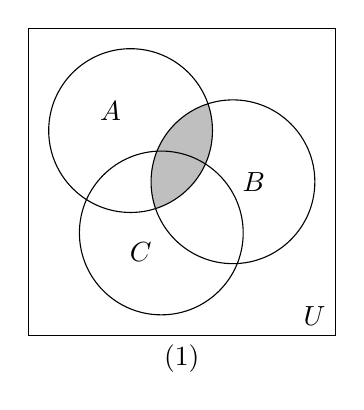
\begin{tikzpicture}[scale = 1.3]
    \begin{scope}
        \clip (1,2) circle (0.8);
        \clip (2,1.5) circle (0.8);     
        \fill [gray!50] (0,0) rectangle (3,3);
    \end{scope}
    \draw (1,2) circle (0.8) node [above left] {$A$};
    \draw (2,1.5) circle (0.8) node [right] {$B$};
    \draw (1.3,1) circle (0.8) node [below left] {$C$};
    \draw (3,0) node [above left] {$U$} rectangle (0,3);
    \draw (1.5,0) node [below] {(1)};   
\end{tikzpicture}
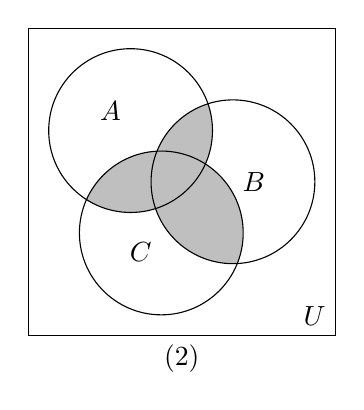
\begin{tikzpicture}[scale = 1.3]
    \begin{scope}
        \clip (1,2) circle (0.8);
        \clip (2,1.5) circle (0.8);     
        \fill [gray!50] (0,0) rectangle (3,3);
    \end{scope}
    \begin{scope}
        \clip (1.3,1) circle (0.8);
        \clip (2,1.5) circle (0.8);     
        \fill [gray!50] (0,0) rectangle (3,3);
    \end{scope}
    \begin{scope}
        \clip (1.3,1) circle (0.8);
        \clip (1,2) circle (0.8);     
        \fill [gray!50] (0,0) rectangle (3,3);
    \end{scope}
    \draw (1,2) circle (0.8) node [above left] {$A$};
    \draw (2,1.5) circle (0.8) node [right] {$B$};
    \draw (1.3,1) circle (0.8) node [below left] {$C$};
    \draw (3,0) node [above left] {$U$} rectangle (0,3);
    \draw (1.5,0) node [below] {(2)};   
\end{tikzpicture}
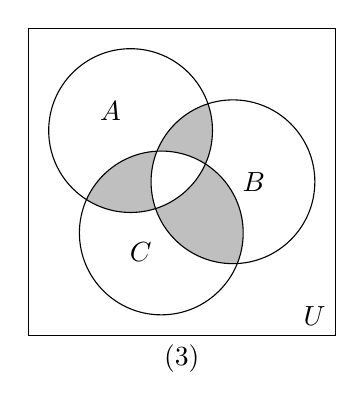
\begin{tikzpicture}[scale = 1.3]
    \begin{scope}[even odd rule]
        \clip (1,2) circle (0.8) (2,1.5) circle (0.8) (1.3,1) circle (0.8) (0,0) rectangle (3,3);
        \fill [gray!50] (1,2) circle (0.8);
        \fill [gray!50] (2,1.5) circle (0.8);
    \end{scope}
    \draw (1,2) circle (0.8) node [above left] {$A$};
    \draw (2,1.5) circle (0.8) node [right] {$B$};
    \draw (1.3,1) circle (0.8) node [below left] {$C$};
    \draw (3,0) node [above left] {$U$} rectangle (0,3);
    \draw (1.5,0) node [below] {(3)};   
\end{tikzpicture}
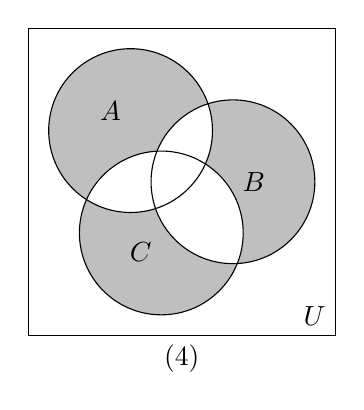
\begin{tikzpicture}[scale = 1.3]
    \begin{scope}[even odd rule]
        \clip (1,2) circle (0.8) (0,0) rectangle (3,3);
        \clip (2,1.5) circle (0.8) (0,0) rectangle (3,3);
        \fill [gray!50] (1.3,1) circle (0.8);
    \end{scope}
    \begin{scope}[even odd rule]
        \clip (1.3,1) circle (0.8) (0,0) rectangle (3,3);
        \clip (2,1.5) circle (0.8) (0,0) rectangle (3,3);
        \fill [gray!50] (1,2) circle (0.8);
    \end{scope}
    \begin{scope}[even odd rule]
        \clip (1,2) circle (0.8) (0,0) rectangle (3,3);
        \clip (1.3,1) circle (0.8) (0,0) rectangle (3,3);
        \fill [gray!50] (2,1.5) circle (0.8);
    \end{scope}
    \draw (1,2) circle (0.8) node [above left] {$A$};
    \draw (2,1.5) circle (0.8) node [right] {$B$};
    \draw (1.3,1) circle (0.8) node [below left] {$C$};
    \draw (3,0) node [above left] {$U$} rectangle (0,3);
    \draw (1.5,0) node [below] {(4)};   
\end{tikzpicture}
\end{center} 
1. \blank{200};2. \blank{200};\\ 
3. \blank{200};4. \blank{200}.


关联目标:

暂未关联目标

答案: 暂无答案

解答或提示: 暂无解答与提示

使用记录:

2016届11班	\fcolorbox[rgb]{0,0,0}{1.000,0.000,0}{1.000}	\fcolorbox[rgb]{0,0,0}{1.000,0.102,0}{0.949}	\fcolorbox[rgb]{0,0,0}{1.000,0.666,0}{0.667}	\fcolorbox[rgb]{0,0,0}{1.000,0.564,0}{0.718}

2016届12班	\fcolorbox[rgb]{0,0,0}{1.000,0.000,0}{1.000}	\fcolorbox[rgb]{0,0,0}{1.000,0.052,0}{0.974}	\fcolorbox[rgb]{0,0,0}{1.000,0.974,0}{0.513}	\fcolorbox[rgb]{0,0,0}{1.000,0.820,0}{0.590}


出处: 2016届创新班作业	1106-集合的运算
\item { (001013)}已知集合$M=\{(x,y)|y=x+1, \ x \in \mathbf{R}\}$, $N=\{(x,y)|y=-x^2+4x,\  x \in \mathbf{R}\}$,
则$M \cap N=$\blank{80}.


关联目标:

暂未关联目标

答案: 暂无答案

解答或提示: 暂无解答与提示

使用记录:

2016届11班	\fcolorbox[rgb]{0,0,0}{1.000,0.358,0}{0.821}

2016届12班	\fcolorbox[rgb]{0,0,0}{1.000,0.102,0}{0.949}


出处: 2016届创新班作业	1106-集合的运算
\item { (001014)}已知集合$M=\{y|y=x+1, \ x \in \mathbf{R}\}$, $N=\{y|y=-x^2+4x,\  x \in \mathbf{R}\}$,
则$M \cap N=$\blank{80}.


关联目标:

暂未关联目标

答案: 暂无答案

解答或提示: 暂无解答与提示

使用记录:

2016届11班	\fcolorbox[rgb]{0,0,0}{0.820,1.000,0}{0.410}

2016届12班	\fcolorbox[rgb]{0,0,0}{0.616,1.000,0}{0.308}


出处: 2016届创新班作业	1106-集合的运算
\item { (001015)}已知集合$A=\{x|\ x^2+px+q=0\}$, $B=\{x|\ x^2-x+r=0\}$, 且$A\cap B=\{-1\}$, $A\cup B=\{-1,2\}$, 求实数$p,q,r$的值.


关联目标:

暂未关联目标

答案: 暂无答案

解答或提示: 暂无解答与提示

使用记录:

2016届11班	\fcolorbox[rgb]{0,0,0}{1.000,0.666,0}{0.667}

2016届12班	\fcolorbox[rgb]{0,0,0}{1.000,0.820,0}{0.590}


出处: 2016届创新班作业	1106-集合的运算
\item { (001016)}已知集合$A=\{1,2\}$, $B=\{x|mx^2+2mx-1<0, x \in\mathbf{R}\}$. 已知$A \cap B=\{1\}$, 求实数$m$的取值范围.


关联目标:

暂未关联目标

答案: 暂无答案

解答或提示: 暂无解答与提示

使用记录:

2016届11班	\fcolorbox[rgb]{0,0,0}{1.000,0.410,0}{0.795}

2016届12班	\fcolorbox[rgb]{0,0,0}{1.000,0.616,0}{0.692}


出处: 2016届创新班作业	1106-集合的运算
\item { (001017)}设$A,B$是两个集合, 求证: ``$A\cap B=A$''当且仅当``$A \subseteq B$''.(用文氏图画一下并不算证明)


关联目标:

暂未关联目标

答案: 暂无答案

解答或提示: 暂无解答与提示

使用记录:

2016届11班	\fcolorbox[rgb]{0,0,0}{0.512,1.000,0}{0.256}

2016届12班	\fcolorbox[rgb]{0,0,0}{0.358,1.000,0}{0.179}


出处: 2016届创新班作业	1106-集合的运算
\item { (001029)}设$f(x)$是$m$次多项式, $g(x)$是$n$次多项式, $m,n$均为正整数. 判断下列命题的真假(T or F).\\ 
\blank{30} (1) 多项式$-2f(x)$的次数为$m$;\\ 
\blank{30} (2) 多项式$f(x)+g(x)$的次数为$\max\{m,n\}$($\max$表示集合中较大的那个数);\\ 
\blank{30} (3) 多项式$f(x)\times g(x)$的次数为$m+n$;\\ 
\blank{30} (4) 多项式$[f(x)]^2+f(x)+1$的次数为$2m$;


关联目标:

暂未关联目标

答案: 暂无答案

解答或提示: 暂无解答与提示

使用记录:

2016届11班	\fcolorbox[rgb]{0,0,0}{1.000,0.000,0}{1.000}	\fcolorbox[rgb]{0,0,0}{1.000,0.462,0}{0.769}	\fcolorbox[rgb]{0,0,0}{1.000,0.102,0}{0.949}	\fcolorbox[rgb]{0,0,0}{1.000,0.102,0}{0.949}

2016届12班	\fcolorbox[rgb]{0,0,0}{1.000,0.000,0}{1.000}	\fcolorbox[rgb]{0,0,0}{1.000,0.512,0}{0.744}	\fcolorbox[rgb]{0,0,0}{1.000,0.000,0}{1.000}	\fcolorbox[rgb]{0,0,0}{1.000,0.102,0}{0.949}


出处: 2016届创新班作业	1110-多项式的有关概念
\item { (001152)}设$f:\ A\rightarrow B$是集合$A$到集合$B$的映射, 则以下正确的是\blank{50}
\twoch{$A$中每一元素在$B$中必有像}{$B$中每一元素在$A$中必有原像}{$B$中每一元素在$A$中的原像是唯一的}{$A$中的不同元素的像必不同}


关联目标:

暂未关联目标

答案: 暂无答案

解答或提示: 暂无解答与提示

使用记录:

2016届11班	\fcolorbox[rgb]{0,0,0}{1.000,0.052,0}{0.974}

2016届12班	\fcolorbox[rgb]{0,0,0}{1.000,0.052,0}{0.974}


出处: 2016届创新班作业	1130-对应与映射
\item { (001153)}集合$A=\{1,2,3\}$, 集合$B=\{1,4\}$, 则可建立从$A$到$B$的不同映射共\blank{30}种, 从$B$到$A$的不同映射共\blank{30}种.


关联目标:

暂未关联目标

答案: 暂无答案

解答或提示: 暂无解答与提示

使用记录:

2016届11班	\fcolorbox[rgb]{0,0,0}{1.000,0.316,0}{0.842}

2016届12班	\fcolorbox[rgb]{0,0,0}{1.000,0.158,0}{0.921}


出处: 2016届创新班作业	1130-对应与映射
\item { (001159)}设集合$A=\{-1, 0, 1\}$, $B=\{2,3,4,5,6\}$, 映射$f:\ A\rightarrow B$, 对任意$x\in A$, 都有$x+f(x)+xf(x)$是奇数. 求满足条件的映射个数.


关联目标:

暂未关联目标

答案: 暂无答案

解答或提示: 暂无解答与提示

使用记录:

2016届11班	\fcolorbox[rgb]{0,0,0}{1.000,0.894,0}{0.553}

2016届12班	\fcolorbox[rgb]{0,0,0}{1.000,0.790,0}{0.605}


出处: 2016届创新班作业	1130-对应与映射
\item { (001222)}是非题, 在每个命题之前的横线上写上``T''或``F''即可, 不用写任何原因.\\ 
已知$y=f(x)$是定义在区间$[-1,1]$上的函数.\\ 
\blank{25}(1) 如果$f(x)$是奇函数, 则$f(x)$要么是增函数, 要么是减函数;\\ 
\blank{25}(2) 如果$f(x)$是偶函数, 则$f(x)$既不是增函数, 又不是减函数;\\ 
\blank{25}(3) 如果$f(x)$是奇函数, 且在$[0,1]$上递增, 那么$f(x)$在$[-1,0]$上也递增;\\ 
\blank{25}(4) 如果$f(x)$是奇函数, 且在$[0,1]$上递增, 那么$f(x)$在$[-1,1]$上也递增;\\ 
\blank{25}(5) 如果$f(x)$在$[-1,0),[-\dfrac{1}{2},\dfrac{1}{2}],(0,1]$上都是递增的, 那么$f(x)$ 在$[-1,1]$上也递增.


关联目标:

暂未关联目标

答案: 暂无答案

解答或提示: 暂无解答与提示

使用记录:

2016届11班	\fcolorbox[rgb]{0,0,0}{1.000,0.052,0}{0.974}	\fcolorbox[rgb]{0,0,0}{1.000,0.052,0}{0.974}	\fcolorbox[rgb]{0,0,0}{1.000,0.000,0}{1.000}	\fcolorbox[rgb]{0,0,0}{1.000,0.210,0}{0.895}	\fcolorbox[rgb]{0,0,0}{1.000,0.052,0}{0.974}

2016届12班	\fcolorbox[rgb]{0,0,0}{1.000,0.158,0}{0.921}	\fcolorbox[rgb]{0,0,0}{1.000,0.368,0}{0.816}	\fcolorbox[rgb]{0,0,0}{1.000,0.000,0}{1.000}	\fcolorbox[rgb]{0,0,0}{1.000,0.210,0}{0.895}	\fcolorbox[rgb]{0,0,0}{1.000,0.052,0}{0.974}


出处: 2016届创新班作业	1141-更多奇偶性与单调性的练习
\item { (001223)}是非题, 在每个命题之前的横线上写上``T''或``F''即可, 不用写任何原因.\\ 
已知$y=f(x)$是定义在$[-1,1]$上的偶函数, 在$[0,1]$上递增.\\ 
\blank{25}(1) $f(\dfrac{1}{2})>f(-\dfrac{1}{3})$;\\ 
\blank{25}(2) $f(a)>f(b)$当且仅当$a>b$;\\ 
\blank{25}(3) $f(a)>f(b)$当且仅当$|a|>|b|$;\\ 
\blank{25}(4) $f(a)>f(b)$当且仅当$1\ge |a|>|b|$.


关联目标:

暂未关联目标

答案: 暂无答案

解答或提示: 暂无解答与提示

使用记录:

2016届11班	\fcolorbox[rgb]{0,0,0}{1.000,0.000,0}{1.000}	\fcolorbox[rgb]{0,0,0}{1.000,0.000,0}{1.000}	\fcolorbox[rgb]{0,0,0}{1.000,0.684,0}{0.658}	\fcolorbox[rgb]{0,0,0}{1.000,0.106,0}{0.947}

2016届12班	\fcolorbox[rgb]{0,0,0}{1.000,0.052,0}{0.974}	\fcolorbox[rgb]{0,0,0}{1.000,0.000,0}{1.000}	\fcolorbox[rgb]{0,0,0}{1.000,0.368,0}{0.816}	\fcolorbox[rgb]{0,0,0}{1.000,0.052,0}{0.974}


出处: 2016届创新班作业	1141-更多奇偶性与单调性的练习
\item { (001233)}求下列函数零点的集合, 并说明理由.\\ 
(1) 函数$f(x)=x^3+3x+1,x\in\mathbf{Z}$;\\ 
(2) 函数$f(x)=x^3-3x+1,x\in\mathbf{Z}$.


关联目标:

暂未关联目标

答案: 暂无答案

解答或提示: 暂无解答与提示

使用记录:

2016届11班	\fcolorbox[rgb]{0,0,0}{1.000,0.256,0}{0.872}	\fcolorbox[rgb]{0,0,0}{1.000,0.462,0}{0.769}

2016届12班	\fcolorbox[rgb]{0,0,0}{1.000,0.162,0}{0.919}	\fcolorbox[rgb]{0,0,0}{1.000,0.270,0}{0.865}


出处: 2016届创新班作业	1143-介值定理与函数的零点
\item { (001366)}判断下列命题的真假, 在横线上用``{\rm T}''或``{\rm F}''表示.
\begin{enumerate}[\blank{30}(1)]
\item 已知$A,B$均大于$0^\circ$而小于$180^\circ$. 如果$A>B$, 那么$\sin A>\sin B$;\\ 
\item 已知$A,B$均大于$0^\circ$而小于$180^\circ$. 如果$\sin A>\sin B$, 那么$ A> B$;\\ 
\item 已知$A,B$是同一个三角形的两个内角. 如果$A>B$, 那么$\sin A>\sin B$;\\ 
\item 已知$A,B$是同一个三角形的两个内角. 如果$\sin A>\sin B$, 那么$A>B$.\\ 
\end{enumerate}


关联目标:

暂未关联目标

答案: 暂无答案

解答或提示: 暂无解答与提示

使用记录:

2016届11班	\fcolorbox[rgb]{0,0,0}{1.000,0.000,0}{1.000}	\fcolorbox[rgb]{0,0,0}{1.000,0.052,0}{0.974}	\fcolorbox[rgb]{0,0,0}{1.000,0.154,0}{0.923}	\fcolorbox[rgb]{0,0,0}{1.000,0.052,0}{0.974}

2016届12班	\fcolorbox[rgb]{0,0,0}{1.000,0.052,0}{0.974}	\fcolorbox[rgb]{0,0,0}{1.000,0.000,0}{1.000}	\fcolorbox[rgb]{0,0,0}{1.000,0.000,0}{1.000}	\fcolorbox[rgb]{0,0,0}{1.000,0.052,0}{0.974}


出处: 2016届创新班作业	2101-正弦定理与余弦定理
\item { (001392)}分别用角度制和弧度制写出始边在$x$轴的正半轴上, 终边在下列位置的角的集合.\\ 
例如: $x$轴的正半轴: 角度制\underline{$360^\circ \cdot k, \ k\in \mathbf{Z}$}; 弧度制\underline{$2k\pi, \ k\in \mathbf{Z}$}.
\begin{enumerate}[(1)]
\item $x$轴的负半轴: 角度制\blank{100}; 弧度制\blank{100};\\ 
\item $y$轴的正半轴: 角度制\blank{100}; 弧度制\blank{100};\\ 
\item $y$轴的负半轴: 角度制\blank{100}; 弧度制\blank{100};\\ 
\item $x$轴: 角度制\blank{100}; 弧度制\blank{100};\\ 
\item $y$轴: 角度制\blank{100}; 弧度制\blank{100};\\ 
\item 坐标轴: 角度制\blank{100}; 弧度制\blank{100};\\ 
\item 坐标轴的角平分线: 角度制\blank{100}; 弧度制\blank{100};\\ 
\item 直线$y=\sqrt{3}x$: 角度制\blank{100}; 弧度制\blank{100}.\\ 
\end{enumerate}


关联目标:

暂未关联目标

答案: 暂无答案

解答或提示: 暂无解答与提示

使用记录:

2016届11班	\fcolorbox[rgb]{0,0,0}{1.000,0.000,0}{1.000}	\fcolorbox[rgb]{0,0,0}{1.000,0.000,0}{1.000}	\fcolorbox[rgb]{0,0,0}{1.000,0.154,0}{0.923}	\fcolorbox[rgb]{0,0,0}{1.000,0.000,0}{1.000}	\fcolorbox[rgb]{0,0,0}{1.000,0.000,0}{1.000}	\fcolorbox[rgb]{0,0,0}{1.000,0.000,0}{1.000}	\fcolorbox[rgb]{0,0,0}{1.000,0.154,0}{0.923}	\fcolorbox[rgb]{0,0,0}{1.000,0.256,0}{0.872}

2016届12班	\fcolorbox[rgb]{0,0,0}{1.000,0.000,0}{1.000}	\fcolorbox[rgb]{0,0,0}{1.000,0.052,0}{0.974}	\fcolorbox[rgb]{0,0,0}{1.000,0.106,0}{0.947}	\fcolorbox[rgb]{0,0,0}{1.000,0.052,0}{0.974}	\fcolorbox[rgb]{0,0,0}{1.000,0.000,0}{1.000}	\fcolorbox[rgb]{0,0,0}{1.000,0.000,0}{1.000}	\fcolorbox[rgb]{0,0,0}{1.000,0.106,0}{0.947}	\fcolorbox[rgb]{0,0,0}{1.000,0.316,0}{0.842}


出处: 2016届创新班作业	2105-弧度制与任意角[2]
\item { (001393)}\begin{enumerate}[(1)]
\item 终边和$\dfrac{\pi}{3}$的终边重合的角的集合为\blank{80}; 终边和$\dfrac{\pi}{3}$的终边垂直的角的集合为\blank{80};\\ 
\item $1$弧度角的终边逆时针旋转$2$弧度, 再顺时针旋转$3$弧度, 再逆时针旋转$4$弧度, 再逆时针旋转$5$弧度后, 所得角的大小为\blank{30}; 与其终边相同的角的集合为\blank{80}.\\ 
\item 终边和$\dfrac{\pi}{3}$的终边关于$y$轴对称的角的集合为\blank{80}, 其中在$[-\pi,\pi)$内的角有\blank{30};\\ 
\item 终边和$\dfrac{\pi}{3}$的终边关于$x$轴对称的角的集合为\blank{80}, 其中在$[-\pi,\pi)$内的角有\blank{30};\\ 
\item 终边和$\dfrac{\pi}{3}$的终边关于直线$y=x$对称的角的集合为\blank{80}, 其中在$[-\pi,\pi)$内的角有\blank{30};\\ 
\item 终边和$\dfrac{\pi}{3}$的终边关于直线$y=-x$对称的角的集合为\blank{80}, 其中在$[-\pi,\pi)$内的角有\blank{30};\\ 
\item 终边和$\dfrac{\pi}{3}$的终边关于直线$y=\dfrac{\sqrt{3}}{3}x$对称的角的集合为\blank{80}, 其中在$[-\pi,\pi)$内的角有\blank{30}.\\ 
\item 若角$\alpha$与角$\beta$的终边关于角$\dfrac{\pi}{5}$的终边所在直线对称, 则角$\alpha$与角$\beta$ 满足的关系式为\blank{80}.\\ 
\end{enumerate}


关联目标:

暂未关联目标

答案: 暂无答案

解答或提示: 暂无解答与提示

使用记录:

2016届11班	\fcolorbox[rgb]{0,0,0}{1.000,0.616,0}{0.692}	\fcolorbox[rgb]{0,0,0}{1.000,0.770,0}{0.615}	\fcolorbox[rgb]{0,0,0}{1.000,0.102,0}{0.949}	\fcolorbox[rgb]{0,0,0}{1.000,0.154,0}{0.923}	\fcolorbox[rgb]{0,0,0}{1.000,0.206,0}{0.897}	\fcolorbox[rgb]{0,0,0}{1.000,0.256,0}{0.872}	\fcolorbox[rgb]{0,0,0}{1.000,0.102,0}{0.949}	\fcolorbox[rgb]{0,0,0}{1.000,0.616,0}{0.692}

2016届12班	\fcolorbox[rgb]{0,0,0}{1.000,0.894,0}{0.553}	\fcolorbox[rgb]{0,0,0}{1.000,0.474,0}{0.763}	\fcolorbox[rgb]{0,0,0}{1.000,0.052,0}{0.974}	\fcolorbox[rgb]{0,0,0}{1.000,0.316,0}{0.842}	\fcolorbox[rgb]{0,0,0}{1.000,0.158,0}{0.921}	\fcolorbox[rgb]{0,0,0}{1.000,0.578,0}{0.711}	\fcolorbox[rgb]{0,0,0}{1.000,0.316,0}{0.842}	\fcolorbox[rgb]{0,0,0}{1.000,0.632,0}{0.684}


出处: 2016届创新班作业	2105-弧度制与任意角[2]
\item { (001394)}如果$\alpha$是第三象限角, 将$\alpha$的范围用集合表示出来. 将$\dfrac{\alpha}{2}$的范围用集合表示出来, 并且在直角坐标系中用阴影表示$\dfrac{\alpha}{2}$的范围(注意边界若取得到用实线, 若取不到用虚线表示).


关联目标:

暂未关联目标

答案: 暂无答案

解答或提示: 暂无解答与提示

使用记录:

2016届11班	\fcolorbox[rgb]{0,0,0}{1.000,0.820,0}{0.590}

2016届12班	\fcolorbox[rgb]{0,0,0}{1.000,0.422,0}{0.789}


出处: 2016届创新班作业	2105-弧度制与任意角[2]
\item { (001395)}如果$\alpha$是第二象限角, 将$\alpha$的范围用集合表示出来. 将$3\alpha$和$\dfrac{\alpha}{3}$的范围用集合表示出来, 并且在直角坐标系中分别用阴影表示$\alpha$, $3\alpha$和$\dfrac{\alpha}{3}$的范围(注意边界若取得到用实线, 若取不到用虚线表示).


关联目标:

暂未关联目标

答案: 暂无答案

解答或提示: 暂无解答与提示

使用记录:

2016届11班	\fcolorbox[rgb]{0,0,0}{1.000,0.924,0}{0.538}

2016届12班	\fcolorbox[rgb]{0,0,0}{1.000,0.736,0}{0.632}


出处: 2016届创新班作业	2105-弧度制与任意角[2]
\item { (001414)}已知集合$M=\left\{x\left|x=\cos\dfrac{k\pi}{3}, \ k \in \mathbf{Z}\right.\right\}$, $N=\left\{y\left|y=\sin\dfrac{2n+1}{6}\pi,\ n \in \mathbf{Z}\right.\right\}$, 则$M$\blank{20}$N$(填入``$\subsetneqq$'',``$=$'',``$\supsetneqq$''之一).


关联目标:

暂未关联目标

答案: 暂无答案

解答或提示: 暂无解答与提示

使用记录:

2016届11班	\fcolorbox[rgb]{0,0,0}{1.000,0.368,0}{0.816}

2016届12班	\fcolorbox[rgb]{0,0,0}{1.000,0.368,0}{0.816}


出处: 2016届创新班作业	2108-诱导公式
\item { (001433)}已知在$\triangle ABC$中, 有以下三个命题:\\ 
P: $\triangle ABC$是钝角三角形;\\ 
Q: $\tan A\tan B<1$;\\ 
R: $\sin A\sin B<\cos A\cos B$.\\ 
(1) $P$是$Q$的\blank{50}条件; $Q$是$R$的\blank{50}条件; $R$是$P$的\blank{50}条件.
(填``充分必要'', ``充分非必要'', ``必要非充分'', ``既非充分又非必要''中的一个.)\\ 
(2) 对$P$与$Q$的关系作详细证明.


关联目标:

暂未关联目标

答案: 暂无答案

解答或提示: 暂无解答与提示

使用记录:

2016届11班	\fcolorbox[rgb]{0,0,0}{1.000,0.512,0}{0.744}	\fcolorbox[rgb]{0,0,0}{1.000,0.718,0}{0.641}

2016届12班	\fcolorbox[rgb]{0,0,0}{0.894,1.000,0}{0.447}	\fcolorbox[rgb]{0,0,0}{1.000,0.790,0}{0.605}


出处: 2016届创新班作业	2110-和差角公式
\item { (001437)}命题``$\alpha$, $\beta$使式$\tan\alpha+\tan\beta$有意义且值为$0$''是
命题``$\alpha$, $\beta$使式$\tan(\alpha+\beta)$有意义且值为$0$''的\blank{50}条件.
(填``充分必要'', ``充分非必要'', ``必要非充分'', ``既非充分又非必要''中的一个.)


关联目标:

暂未关联目标

答案: 暂无答案

解答或提示: 暂无解答与提示

使用记录:

2016届11班	\fcolorbox[rgb]{0,0,0}{1.000,1.000,0}{0.500}

2016届12班	\fcolorbox[rgb]{0,0,0}{1.000,0.790,0}{0.605}


出处: 2016届创新班作业	2111-两角和与差的正切公式
\item { (001491)}判断下列命题的真假, 真命题用``{\rm T}''表示, 假命题用``{\rm F}''表示.\\ 
\begin{enumerate}[\blank{30}(1)]
\item 设函数$y=f(x)$的定义域为$\mathbf{R}$, 若$1$是它的一个周期, 则$2$也是它的一个周期;\\ 
\item 设函数$y=f(x)$的定义域为$D$, 若$1$是它的一个周期, 则$2$也是它的一个周期;\\ 
\item 设函数$y=f(x)$的定义域为$\mathbf{R}$, 若$1$是它的一个周期, 则$-1$也是它的一个周期;\\ 
\item 设函数$y=f(x)$的定义域为$D$, 若$1$是它的一个周期, 则$-1$也是它的一个周期;\\ 
\item 设函数$f(x)$的定义域为$\mathbf{R}$, 若$1$是它的一个周期, 则$\sqrt{2}$一定不是它的周期;\\ 
\item 设函数$f(x)$的定义域为$\mathbf{R}$, 且$f(x)$不是常数函数, 若$1$是它的一个周期, 则$\sqrt{2}$一定不是它的周期;\\ 
\item 定义在$\mathbf{R}$上的常数函数是周期函数;\\ 
\item 奇函数一定是周期函数;\\ 
\item 奇函数一定不是周期函数;\\ 
\item 偶函数一定是周期函数;\\ 
\item 偶函数一定不是周期函数;\\ 
\item 单调函数一定不是周期函数;\\ 
\item 一定不存在正实数$M$, 使得周期函数$y=f(x)$的定义域包含于区间$[-M,M]$;\\ 
\item 如果$1$是函数$y=f(x)$, $y=g(x)$的周期, 且$f(x)$与$g(x)$定义域的交集非空, 那么$1$也是$y=f(x)+g(x)$的周期;\\ 
\item 设$f(x),g(x)$的定义域均为$\mathbf{R}$, 若$1$是函数$y=f(x)$的周期, 则$1$是函数$y=f(g(x))$的周期;\\ 
\item 设$f(x),g(x)$的定义域均为$\mathbf{R}$, 若$1$是函数$y=g(x)$的周期, 则$1$是函数$y=f(g(x))$的周期;\\ 
\item $y=\sin x,\ x\in (-\infty,0)\cup (0,+\infty)$是周期函数;\\ 
\item $y=\sin x,\ x\in (0,+\infty)$是周期函数;\\ 
\item 周期函数一定有最大值和最小值;\\ 
\item 定义域为$\mathbf{R}$的周期函数一定有最大值和最小值.\\ 
\end{enumerate}


关联目标:

暂未关联目标

答案: 暂无答案

解答或提示: 暂无解答与提示

使用记录:

2016届11班	\fcolorbox[rgb]{0,0,0}{1.000,0.000,0}{1.000}	\fcolorbox[rgb]{0,0,0}{1.000,0.512,0}{0.744}	\fcolorbox[rgb]{0,0,0}{1.000,0.000,0}{1.000}	\fcolorbox[rgb]{0,0,0}{1.000,0.154,0}{0.923}	\fcolorbox[rgb]{0,0,0}{1.000,0.000,0}{1.000}	\fcolorbox[rgb]{0,0,0}{0.256,1.000,0}{0.128}	\fcolorbox[rgb]{0,0,0}{1.000,0.000,0}{1.000}	\fcolorbox[rgb]{0,0,0}{1.000,0.000,0}{1.000}	\fcolorbox[rgb]{0,0,0}{1.000,0.154,0}{0.923}	\fcolorbox[rgb]{0,0,0}{1.000,0.000,0}{1.000}	\fcolorbox[rgb]{0,0,0}{1.000,0.000,0}{1.000}	\fcolorbox[rgb]{0,0,0}{1.000,0.052,0}{0.974}	\fcolorbox[rgb]{0,0,0}{1.000,0.358,0}{0.821}	\fcolorbox[rgb]{0,0,0}{0.974,1.000,0}{0.487}	\fcolorbox[rgb]{0,0,0}{1.000,0.256,0}{0.872}	\fcolorbox[rgb]{0,0,0}{1.000,0.358,0}{0.821}	\fcolorbox[rgb]{0,0,0}{1.000,0.052,0}{0.974}	\fcolorbox[rgb]{0,0,0}{1.000,0.102,0}{0.949}	\fcolorbox[rgb]{0,0,0}{1.000,0.206,0}{0.897}	\fcolorbox[rgb]{0,0,0}{1.000,0.820,0}{0.590}

2016届12班	\fcolorbox[rgb]{0,0,0}{1.000,0.000,0}{1.000}	\fcolorbox[rgb]{0,0,0}{1.000,0.264,0}{0.868}	\fcolorbox[rgb]{0,0,0}{1.000,0.000,0}{1.000}	\fcolorbox[rgb]{0,0,0}{1.000,0.052,0}{0.974}	\fcolorbox[rgb]{0,0,0}{1.000,0.000,0}{1.000}	\fcolorbox[rgb]{0,0,0}{0.264,1.000,0}{0.132}	\fcolorbox[rgb]{0,0,0}{1.000,0.052,0}{0.974}	\fcolorbox[rgb]{0,0,0}{1.000,0.000,0}{1.000}	\fcolorbox[rgb]{0,0,0}{1.000,0.052,0}{0.974}	\fcolorbox[rgb]{0,0,0}{1.000,0.000,0}{1.000}	\fcolorbox[rgb]{0,0,0}{1.000,0.052,0}{0.974}	\fcolorbox[rgb]{0,0,0}{1.000,0.106,0}{0.947}	\fcolorbox[rgb]{0,0,0}{1.000,0.474,0}{0.763}	\fcolorbox[rgb]{0,0,0}{1.000,0.684,0}{0.658}	\fcolorbox[rgb]{0,0,0}{1.000,0.316,0}{0.842}	\fcolorbox[rgb]{0,0,0}{1.000,0.578,0}{0.711}	\fcolorbox[rgb]{0,0,0}{1.000,0.368,0}{0.816}	\fcolorbox[rgb]{0,0,0}{1.000,0.000,0}{1.000}	\fcolorbox[rgb]{0,0,0}{1.000,0.000,0}{1.000}	\fcolorbox[rgb]{0,0,0}{1.000,0.264,0}{0.868}


出处: 2016届创新班作业	2117-周期性的概念
\item { (001495)}下列假命题经常被误以为是正确的, 请对每个命题举出一个反例(不需要论证):\\ 
(1) 若$f(x)$与$g(x)$的最小正周期均为$T$, 则$f(x)g(x)$的最小正周期为$T$;\\ 
(2) 若$f(x)$与$g(x)$的最小正周期均为$T$, 则$f(x)+g(x)$的最小正周期为$T$.


关联目标:

暂未关联目标

答案: 暂无答案

解答或提示: 暂无解答与提示

使用记录:

2016届11班	\fcolorbox[rgb]{0,0,0}{1.000,0.358,0}{0.821}	\fcolorbox[rgb]{0,0,0}{1.000,0.154,0}{0.923}

2016届12班	\fcolorbox[rgb]{0,0,0}{1.000,0.210,0}{0.895}	\fcolorbox[rgb]{0,0,0}{1.000,0.158,0}{0.921}


出处: 2016届创新班作业	2118-周期性与最小正周期
\item { (001503)}使函数$y=3-\cos 2x$取到最小值的所有$x$的集合是\blank{80}.


关联目标:

暂未关联目标

答案: 暂无答案

解答或提示: 暂无解答与提示

使用记录:

2016届11班	\fcolorbox[rgb]{0,0,0}{1.000,0.154,0}{0.923}

2016届12班	\fcolorbox[rgb]{0,0,0}{1.000,0.264,0}{0.868}


出处: 2016届创新班作业	2119-正弦函数与余弦函数的基本性质
\item { (001543)}已知函数$y=A\sin(\omega x+\varphi)$的振幅是$3$, 最小正周期为$\dfrac{2\pi}{7}$,
初相为$\dfrac{\pi}{6}$, 则使这个函数取到最大值的$x$的集合为\blank{80}.


关联目标:

暂未关联目标

答案: 暂无答案

解答或提示: 暂无解答与提示

使用记录:

2016届11班	\fcolorbox[rgb]{0,0,0}{1.000,0.256,0}{0.872}

2016届12班	\fcolorbox[rgb]{0,0,0}{1.000,0.474,0}{0.763}


出处: 2016届创新班作业	2122-正弦型函数
\item { (001592)}用集合的语言表述下列语句, 并用铅笔作出示意图(画直线需用尺).
\begin{enumerate}[(1)]
\item 点$A$在平面$\alpha$上: \blank{80};\\ 
\item 点$B$不在平面$\beta$上: \blank{80};\\ 
\item 平面$\alpha$经过直线$AC$: \blank{80};\\ 
\item 直线$BC$与平面$\alpha$相交于点$C$: \blank{80}.\\ 
\end{enumerate}


关联目标:

暂未关联目标

答案: 暂无答案

解答或提示: 暂无解答与提示

使用记录:

2016届11班	\fcolorbox[rgb]{0,0,0}{1.000,0.000,0}{1.000}	\fcolorbox[rgb]{0,0,0}{1.000,0.000,0}{1.000}	\fcolorbox[rgb]{0,0,0}{1.000,0.718,0}{0.641}	\fcolorbox[rgb]{0,0,0}{1.000,0.462,0}{0.769}

2016届12班	\fcolorbox[rgb]{0,0,0}{1.000,0.000,0}{1.000}	\fcolorbox[rgb]{0,0,0}{1.000,0.000,0}{1.000}	\fcolorbox[rgb]{0,0,0}{1.000,0.378,0}{0.811}	\fcolorbox[rgb]{0,0,0}{1.000,0.432,0}{0.784}


出处: 2016届创新班作业	2201-点线面与立体几何三公理
\item { (001595)}判断下列命题的真假, 在横线上用``T''或``F''表示.
\begin{enumerate}[\blank{30}(1)]
\item 空间任意三点确定一个平面;\\ 
\item 空间任意两条直线确定一个平面;\\ 
\item 空间两条平行直线确定一个平面;\\ 
\item 空间一条直线和不在该直线上的一个点确定一个平面;\\ 
\item 空间一个点和不通过该点的一条直线确定一个平面;\\ 
\item 空间两条没有交点的直线必平行;\\ 
\item 若空间四边形$ABCD$若满足$AB=BC=CD=DA$, 则它一定是菱形;\\ 
\item 若空间的一条直线如果和一对平行直线之一相交, 则一定与另一条也相交;\\ 
\item 若空间三点$A,B,C$若满足$AB^2+BC^2=CA^2$, 则$\triangle ABC$是以$B$为直角顶点的直角三角形;\\ 
\item 若空间三条直线两两相交, 则通过它们中至少两条的平面有且仅有$1$个;\\ 
\item 若空间三条直线两两相交, 则通过它们中至少两条的平面有且仅有$3$个.\\ 
\end{enumerate}


关联目标:

暂未关联目标

答案: 暂无答案

解答或提示: 暂无解答与提示

使用记录:

2016届11班	\fcolorbox[rgb]{0,0,0}{1.000,0.000,0}{1.000}	\fcolorbox[rgb]{0,0,0}{1.000,0.102,0}{0.949}	\fcolorbox[rgb]{0,0,0}{1.000,0.000,0}{1.000}	\fcolorbox[rgb]{0,0,0}{1.000,0.000,0}{1.000}	\fcolorbox[rgb]{0,0,0}{1.000,0.000,0}{1.000}	\fcolorbox[rgb]{0,0,0}{1.000,0.000,0}{1.000}	\fcolorbox[rgb]{0,0,0}{1.000,0.000,0}{1.000}	\fcolorbox[rgb]{0,0,0}{1.000,0.052,0}{0.974}	\fcolorbox[rgb]{0,0,0}{1.000,0.102,0}{0.949}	\fcolorbox[rgb]{0,0,0}{1.000,0.616,0}{0.692}	\fcolorbox[rgb]{0,0,0}{1.000,0.102,0}{0.949}

2016届12班	\fcolorbox[rgb]{0,0,0}{1.000,0.216,0}{0.892}	\fcolorbox[rgb]{0,0,0}{1.000,0.108,0}{0.946}	\fcolorbox[rgb]{0,0,0}{1.000,0.000,0}{1.000}	\fcolorbox[rgb]{0,0,0}{1.000,0.000,0}{1.000}	\fcolorbox[rgb]{0,0,0}{1.000,0.000,0}{1.000}	\fcolorbox[rgb]{0,0,0}{1.000,0.000,0}{1.000}	\fcolorbox[rgb]{0,0,0}{1.000,0.054,0}{0.973}	\fcolorbox[rgb]{0,0,0}{1.000,0.108,0}{0.946}	\fcolorbox[rgb]{0,0,0}{1.000,0.270,0}{0.865}	\fcolorbox[rgb]{0,0,0}{0.864,1.000,0}{0.432}	\fcolorbox[rgb]{0,0,0}{1.000,0.054,0}{0.973}


出处: 2016届创新班作业	2201-点线面与立体几何三公理
\item { (001596)}已知不共线的三点$A,B,C$均在平面$\alpha$上. 证明以下命题(每一步均需说明根据):\\ 
(1) 直线$AB$上的每一点都在平面$\alpha$上;\\ 
(2) 三角形$ABC$的重心$G$在平面$\alpha$上.


关联目标:

暂未关联目标

答案: 暂无答案

解答或提示: 暂无解答与提示

使用记录:

2016届11班	\fcolorbox[rgb]{0,0,0}{1.000,0.154,0}{0.923}	\fcolorbox[rgb]{0,0,0}{1.000,0.564,0}{0.718}

2016届12班	\fcolorbox[rgb]{0,0,0}{1.000,0.216,0}{0.892}	\fcolorbox[rgb]{0,0,0}{1.000,0.486,0}{0.757}


出处: 2016届创新班作业	2201-点线面与立体几何三公理
\item { (001598)}判断下列命题的真假, 在横线上用``T''或``F''表示.
\begin{enumerate}[\blank{30}(1)]
\item 已知$\alpha$, $\beta$是两个平面, $l,m$是两条直线, 若$l\subsetneqq \alpha$, $m\subsetneqq \beta$, 则$l,m$异面;\\ 
\item 已知平面$\alpha,\beta$相交于直线$l$. 若直线$m\subsetneqq \alpha$, $l \parallel m$, 直线$n\subsetneqq \beta$, $l$与$n$相交, 则$m$与$n$异面;\\ 
\item 已知$l,m$是异面直线, 若直线$n\parallel l$, 则$m,n$异面;\\ 
\item 已知$l,m$是异面直线, 若直线$n$和$l$异面, 则$m,n$异面;\\ 
\item 已知$l,m$是异面直线, 若直线$n$和$l$异面, 则$m,n$共面;\\ 
\item 分别和两异面直线都相交的两直线一定是异面直线;\\ 
\item 分别和两异面直线相交的两直线不可能是平行直线;\\ 
\item 正方体的任意两条对角线(指相对顶点, 不同时出现在六个表面的任何一个上的顶点的连线)相交.\\ 
\end{enumerate}


关联目标:

暂未关联目标

答案: 暂无答案

解答或提示: 暂无解答与提示

使用记录:

2016届11班	\fcolorbox[rgb]{0,0,0}{1.000,0.000,0}{1.000}	\fcolorbox[rgb]{0,0,0}{1.000,0.000,0}{1.000}	\fcolorbox[rgb]{0,0,0}{1.000,0.000,0}{1.000}	\fcolorbox[rgb]{0,0,0}{1.000,0.000,0}{1.000}	\fcolorbox[rgb]{0,0,0}{1.000,0.000,0}{1.000}	\fcolorbox[rgb]{0,0,0}{1.000,0.052,0}{0.974}	\fcolorbox[rgb]{0,0,0}{1.000,0.770,0}{0.615}	\fcolorbox[rgb]{0,0,0}{1.000,0.154,0}{0.923}

2016届12班	\fcolorbox[rgb]{0,0,0}{1.000,0.000,0}{1.000}	\fcolorbox[rgb]{0,0,0}{1.000,0.000,0}{1.000}	\fcolorbox[rgb]{0,0,0}{1.000,0.000,0}{1.000}	\fcolorbox[rgb]{0,0,0}{1.000,0.000,0}{1.000}	\fcolorbox[rgb]{0,0,0}{1.000,0.000,0}{1.000}	\fcolorbox[rgb]{0,0,0}{1.000,0.054,0}{0.973}	\fcolorbox[rgb]{0,0,0}{1.000,0.594,0}{0.703}	\fcolorbox[rgb]{0,0,0}{1.000,0.000,0}{1.000}


出处: 2016届创新班作业	2202-平行相交与异面
\item { (001605)}判断下列命题的真假, 在横线上用``T''或``F''表示.\\ 
\begin{enumerate}[\blank{30}(1)]
\item 平行四边形一定在一个平面上;\\ 
\item 若直线$a,b,c$满足$a\perp b$, $a\perp c$, 则$b,c$重合或平行;\\ 
\item 存在一个空间四边形$ABCD$, 它的任意两条邻边的夹角均等于$60^\circ$;\\ 
\item 和两条异面直线都平行的直线不存在;\\ 
\item 过空间一点, 与已知直线垂直的直线有且只有一条;\\ 
\item 若$a,b$是异面直线, $b,c$是异面直线, 则$a,c$也是异面直线;\\ 
\item 若$a,b$是相交直线, $b,c$是相交直线, 则$a,c$也是相交直线;\\ 
\item 有三个角是直角的四边形是矩形;\\ 
\item 异面直线$a,b$和另一直线$c$分别所成的角的大小一定不相等.\\ 
\end{enumerate}


关联目标:

暂未关联目标

答案: 暂无答案

解答或提示: 暂无解答与提示

使用记录:

2016届11班	\fcolorbox[rgb]{0,0,0}{1.000,0.102,0}{0.949}	\fcolorbox[rgb]{0,0,0}{1.000,0.000,0}{1.000}	\fcolorbox[rgb]{0,0,0}{1.000,0.052,0}{0.974}	\fcolorbox[rgb]{0,0,0}{1.000,0.000,0}{1.000}	\fcolorbox[rgb]{0,0,0}{1.000,0.462,0}{0.769}	\fcolorbox[rgb]{0,0,0}{1.000,0.000,0}{1.000}	\fcolorbox[rgb]{0,0,0}{1.000,0.000,0}{1.000}	\fcolorbox[rgb]{0,0,0}{1.000,0.410,0}{0.795}	\fcolorbox[rgb]{0,0,0}{1.000,0.102,0}{0.949}

2016届12班	\fcolorbox[rgb]{0,0,0}{1.000,0.000,0}{1.000}	\fcolorbox[rgb]{0,0,0}{1.000,0.000,0}{1.000}	\fcolorbox[rgb]{0,0,0}{1.000,0.106,0}{0.947}	\fcolorbox[rgb]{0,0,0}{1.000,0.158,0}{0.921}	\fcolorbox[rgb]{0,0,0}{0.842,1.000,0}{0.421}	\fcolorbox[rgb]{0,0,0}{1.000,0.000,0}{1.000}	\fcolorbox[rgb]{0,0,0}{1.000,0.000,0}{1.000}	\fcolorbox[rgb]{0,0,0}{1.000,0.790,0}{0.605}	\fcolorbox[rgb]{0,0,0}{1.000,0.000,0}{1.000}


出处: 2016届创新班作业	2204-两直线的关系综合
\item { (001610)}判断下列命题的真假, 并用``{\rm T}''或``{\rm F}''表示:
\begin{enumerate}[\blank{30}(1)]
\item 如果两条直线和同一平面平行, 那么这两直线平行;\\ 
\item 如果两直线和同一平面平行, 那么这两直线平行或相交;\\ 
\item 同时和两异面直线平行的平面有无数个;\\ 
\item 若直线$a\subsetneqq$平面$\alpha$, 直线$b$不在平面$\alpha$内, $a\cap b=\varnothing$, 则$b \parallel \alpha$;\\ 
\item 直线$a\parallel$直线$b$, 直线$b\parallel$平面$\alpha$. 若直线$a$不在$\alpha$内, 则$a\parallel \alpha$;\\ 
\item 直线$a\parallel$平面$\alpha$, 直线$a\subsetneqq$平面$\beta$. 若$\alpha\cap\beta=b$, 则$a\parallel b$;\\ 
\item 过异面直线$a,b$外一点有且仅有一个平面和$a,b$平行;\\ 
\end{enumerate}


关联目标:

暂未关联目标

答案: 暂无答案

解答或提示: 暂无解答与提示

使用记录:

2016届11班	\fcolorbox[rgb]{0,0,0}{1.000,0.000,0}{1.000}	\fcolorbox[rgb]{0,0,0}{1.000,0.000,0}{1.000}	\fcolorbox[rgb]{0,0,0}{1.000,0.000,0}{1.000}	\fcolorbox[rgb]{0,0,0}{1.000,0.102,0}{0.949}	\fcolorbox[rgb]{0,0,0}{1.000,0.052,0}{0.974}	\fcolorbox[rgb]{0,0,0}{1.000,0.052,0}{0.974}	\fcolorbox[rgb]{0,0,0}{0.770,1.000,0}{0.385}

2016届12班	\fcolorbox[rgb]{0,0,0}{1.000,0.000,0}{1.000}	\fcolorbox[rgb]{0,0,0}{1.000,0.000,0}{1.000}	\fcolorbox[rgb]{0,0,0}{1.000,0.000,0}{1.000}	\fcolorbox[rgb]{0,0,0}{1.000,0.052,0}{0.974}	\fcolorbox[rgb]{0,0,0}{1.000,0.052,0}{0.974}	\fcolorbox[rgb]{0,0,0}{1.000,0.000,0}{1.000}	\fcolorbox[rgb]{0,0,0}{1.000,0.894,0}{0.553}


出处: 2016届创新班作业	2205-线面平行
\item { (001621)}已知: $\triangle ABC$所在平面外一点$P$, 直线$PO\perp$平面$ABC$于$O$点. 求证:\\ 
(1) 如果点$P$到$\triangle ABC$的三个顶点的距离相等, 那么点$O$一定是$\triangle ABC$的外心;\\ 
(2) 如果点$P$到$\triangle ABC$的三边所在直线的距离相等, 且$O$在$\triangle ABC$内, 那么点$O$一定是$\triangle ABC$的内心;\\ 
(3) 如果$AP,BP,CP$两两垂直, 那么点$O$一定是$\triangle ABC$的垂心;\\ 
(4) 以上三个命题各自的逆命题是否成立(毋须证明)?


关联目标:

暂未关联目标

答案: 暂无答案

解答或提示: 暂无解答与提示

使用记录:

2016届11班	\fcolorbox[rgb]{0,0,0}{1.000,0.052,0}{0.974}	\fcolorbox[rgb]{0,0,0}{1.000,0.974,0}{0.513}	\fcolorbox[rgb]{0,0,0}{1.000,0.770,0}{0.615}	\fcolorbox[rgb]{0,0,0}{1.000,0.770,0}{0.615}

2016届12班	\fcolorbox[rgb]{0,0,0}{1.000,0.052,0}{0.974}	\fcolorbox[rgb]{0,0,0}{1.000,0.736,0}{0.632}	\fcolorbox[rgb]{0,0,0}{1.000,0.632,0}{0.684}	\fcolorbox[rgb]{0,0,0}{1.000,0.894,0}{0.553}


出处: 2016届创新班作业	2207-线面垂直的应用
\item { (001622)}判断下列命题的真假, 并用``{\rm T}''或``{\rm F}''表示.\\ 
\begin{enumerate}[\blank{30}(1)]
\item 不在平面内的直线上有三个不同点到该平面的距离都相等, 则此直线平行于该平面.\\ 
\item 与不共线三点距离都相等的点有无数个.\\ 
\item 过固定的平面$\alpha$外一固定点$P$引与$\alpha$相交的直线, 使$P$到交点$O$的距离为$1$, 这样的直线不可能有且只有一条.\\ 
\item 过固定的平面$\alpha$外一固定点$P$引与$\alpha$相交的直线, 使$P$到交点$O$的距离为$1$, 这样的直线不可能有且只有两条.\\ 
\item 一平面上有无数个点到另一平面的距离相等, 则这两个平面无公共点.\\ 
\item 过异面直线$m,n$中的$m$且垂直于$n$的平面有且只有一个.\\ 
\item 如果平面$\alpha$和不在平面$\alpha$内的直线$a$都垂直于直线$b$, 那么平面$\alpha$和直线$a$平行.\\ 
\end{enumerate}


关联目标:

暂未关联目标

答案: 暂无答案

解答或提示: 暂无解答与提示

使用记录:

2016届11班	\fcolorbox[rgb]{0,0,0}{1.000,0.000,0}{1.000}	\fcolorbox[rgb]{0,0,0}{1.000,0.052,0}{0.974}	\fcolorbox[rgb]{0,0,0}{1.000,0.102,0}{0.949}	\fcolorbox[rgb]{0,0,0}{1.000,0.102,0}{0.949}	\fcolorbox[rgb]{0,0,0}{1.000,0.052,0}{0.974}	\fcolorbox[rgb]{0,0,0}{1.000,0.154,0}{0.923}	\fcolorbox[rgb]{0,0,0}{1.000,0.000,0}{1.000}

2016届12班	\fcolorbox[rgb]{0,0,0}{1.000,0.052,0}{0.974}	\fcolorbox[rgb]{0,0,0}{1.000,0.000,0}{1.000}	\fcolorbox[rgb]{0,0,0}{1.000,0.106,0}{0.947}	\fcolorbox[rgb]{0,0,0}{1.000,0.000,0}{1.000}	\fcolorbox[rgb]{0,0,0}{1.000,0.106,0}{0.947}	\fcolorbox[rgb]{0,0,0}{1.000,0.158,0}{0.921}	\fcolorbox[rgb]{0,0,0}{1.000,0.000,0}{1.000}


出处: 2016届创新班作业	2208-点与直线到平面的距离
\item { (001629)}判断下列命题的真假, 并用``{\rm T}''或``{\rm F}''表示.\\ 
\begin{enumerate}[\blank{30}(1)]
\item 在正方体$ABCD-A'B'C'D'$中, $BC'$与对角面$BB'D'D$所成的角是$\angle C'BB'$.\\ 
\item 两条异面直线在同一个平面上的射影不可能是两个点.\\ 
\item 已知$P$是三角形$ABC$所在平面外一点, 且$PA=PB$, 则$P$点在平面$ABC$上的射影一定在$AB$的中垂线(在平面$ABC$内)上.\\ 
\item 已知$P$是三角形$ABC$所在平面外一点, 且$PA=PB=PC$, 则$P$点在平面$ABC$上的射影一定在三角形$ABC$内部.\\ 
\item 已知$P$是三角形$ABC$所在平面外一点, 且$PA=PB=PC$, 则$P$点在平面$ABC$上的射影一定不与$A$重合.\\ 
\item 若两直线分别与一平面所成角相等,则两直线平行.\\ 
\item 平面$\alpha$的斜线$a$在平面$\alpha$内的射影是直线$b$, 如果直线$c\perp b$,那么$c\perp a$.\\ 
\item 若平面$\alpha$外两直线$a,b$在$\alpha$上的射影是两相交直线, 则$a$与$b$相交.\\ 
\item 两条异面直线在同一平面上的射影是两条相交或平行直线.\\ 
\item 已知平面$\alpha$有一条斜线$l$, 过平面上一点$A$, 在平面$\alpha$内有且只有一条直线与斜线$l$垂直.\\ 
\end{enumerate}


关联目标:

暂未关联目标

答案: 暂无答案

解答或提示: 暂无解答与提示

使用记录:

2016届11班	\fcolorbox[rgb]{0,0,0}{1.000,0.154,0}{0.923}	\fcolorbox[rgb]{0,0,0}{1.000,0.206,0}{0.897}	\fcolorbox[rgb]{0,0,0}{1.000,0.052,0}{0.974}	\fcolorbox[rgb]{0,0,0}{1.000,0.308,0}{0.846}	\fcolorbox[rgb]{0,0,0}{1.000,0.000,0}{1.000}	\fcolorbox[rgb]{0,0,0}{1.000,0.000,0}{1.000}	\fcolorbox[rgb]{0,0,0}{1.000,0.102,0}{0.949}	\fcolorbox[rgb]{0,0,0}{1.000,0.000,0}{1.000}	\fcolorbox[rgb]{0,0,0}{1.000,0.462,0}{0.769}	\fcolorbox[rgb]{0,0,0}{1.000,0.462,0}{0.769}

2016届12班	\fcolorbox[rgb]{0,0,0}{1.000,0.000,0}{1.000}	\fcolorbox[rgb]{0,0,0}{1.000,0.000,0}{1.000}	\fcolorbox[rgb]{0,0,0}{1.000,0.000,0}{1.000}	\fcolorbox[rgb]{0,0,0}{1.000,0.052,0}{0.974}	\fcolorbox[rgb]{0,0,0}{1.000,0.000,0}{1.000}	\fcolorbox[rgb]{0,0,0}{1.000,0.000,0}{1.000}	\fcolorbox[rgb]{0,0,0}{1.000,0.106,0}{0.947}	\fcolorbox[rgb]{0,0,0}{1.000,0.000,0}{1.000}	\fcolorbox[rgb]{0,0,0}{1.000,0.632,0}{0.684}	\fcolorbox[rgb]{0,0,0}{1.000,0.578,0}{0.711}


出处: 2016届创新班作业	2209-直线与平面所成的角[1]
\item { (001642)}判断下列命题的真假, 并用``{\rm T}''或``{\rm F}''表示.\\ 
\begin{enumerate}[\blank{30}(1)]
\item 过平面$\alpha$外一点, 有且仅有一个平面与平面$\alpha$平行.\\ 
\item 已知直线$l$平行于平面$\alpha$, 过$l$有且仅有一个平面与平面$\alpha$平行.\\ 
\item 已知直线$l$不在平面$\alpha$内, 过$l$有且仅有一个平面与平面$\alpha$平行.\\ 
\item 平面$\alpha$平行于平面$\beta$, $l\subsetneqq \alpha$, $m\subsetneqq \beta$, 则$l,m$平行.\\ 
\item 已知$l,m$是两异面直线, 存在平面$\alpha,\beta$, 满足$l\subsetneqq \alpha$, $m\subsetneqq\beta$, 并且$\alpha\parallel \beta$.\\ 
\item 已知$l,m$是两平行直线, $l\subsetneqq \alpha$, $m\subsetneqq \beta$. 若$l\parallel \beta$, $m\parallel \alpha$, 则$\alpha\parallel \beta$.\\ 
\item 平面$\alpha$与平面$\beta$平行, 当且仅当在$\alpha$内有无穷多条直线与$\beta$ 平行.\\ 
\end{enumerate}


关联目标:

暂未关联目标

答案: 暂无答案

解答或提示: 暂无解答与提示

使用记录:

2016届11班	\fcolorbox[rgb]{0,0,0}{1.000,0.052,0}{0.974}	\fcolorbox[rgb]{0,0,0}{1.000,0.106,0}{0.947}	\fcolorbox[rgb]{0,0,0}{1.000,0.052,0}{0.974}	\fcolorbox[rgb]{0,0,0}{1.000,0.000,0}{1.000}	\fcolorbox[rgb]{0,0,0}{1.000,0.052,0}{0.974}	\fcolorbox[rgb]{0,0,0}{1.000,0.158,0}{0.921}	\fcolorbox[rgb]{0,0,0}{1.000,0.210,0}{0.895}

2016届12班	\fcolorbox[rgb]{0,0,0}{1.000,0.000,0}{1.000}	\fcolorbox[rgb]{0,0,0}{1.000,0.000,0}{1.000}	\fcolorbox[rgb]{0,0,0}{1.000,0.000,0}{1.000}	\fcolorbox[rgb]{0,0,0}{1.000,0.000,0}{1.000}	\fcolorbox[rgb]{0,0,0}{1.000,0.106,0}{0.947}	\fcolorbox[rgb]{0,0,0}{1.000,0.052,0}{0.974}	\fcolorbox[rgb]{0,0,0}{1.000,0.368,0}{0.816}


出处: 2016届创新班作业	2211-两平面的位置关系[1]
\item { (001648)}有下列四个命题: (1) 分别在两个平行平面内的两条直线平行; (2) 若两个平面平行, 则其中一个平面内的直线必平行于另一个平面; (3) 如果一个平面内的两条直线平行于另一个平面, 则这两个平面平行; (4) 如果一个平面内的任何一条直线都平行于另一个平面, 则这两个平面平行.\\ 
其中正确命题的个数是\blank{30}.\\ 
\fourch{1}{2}{3}{4}


关联目标:

暂未关联目标

答案: 暂无答案

解答或提示: 暂无解答与提示

使用记录:

2016届11班	\fcolorbox[rgb]{0,0,0}{1.000,0.052,0}{0.974}

2016届12班	\fcolorbox[rgb]{0,0,0}{1.000,0.106,0}{0.947}


出处: 2016届创新班作业	2212-两平面的位置关系[2]
\item { (001649)}下列命题中不正确的是\blank{30}.\\ 
\onech{垂直于同一条直线的两个平面平行}{垂直于同一个平面的两条直线相互平行}{若一个平面内有无数条直线都平行于另一个平面, 则这两个平面互相平行}{若两个平行平面分别和第三个平面相交, 则它们的交线互相平行}


关联目标:

暂未关联目标

答案: 暂无答案

解答或提示: 暂无解答与提示

使用记录:

2016届11班	\fcolorbox[rgb]{0,0,0}{1.000,0.102,0}{0.949}

2016届12班	\fcolorbox[rgb]{0,0,0}{1.000,0.106,0}{0.947}


出处: 2016届创新班作业	2212-两平面的位置关系[2]
\item { (001650)}有下列四个命题: (1) 若直线$a\parallel$直线$b$, 则$a$和$b$与平面$\alpha$所成的角相等; (2) 若直线$a$和$b$与平面$\alpha$所成的角相等, 则$a\parallel b$; (3) 若$\alpha\parallel \beta$, 则直线$a$与平面$\alpha$, 平面$\beta$所成的角相等; (4) 若平面$\alpha$, 平面$\beta$都与直线$a$平行, 则$\alpha\parallel \beta$.\\ 
其中正确的命题是\blank{30}.\\ 
\fourch{(1)(3)}{(1)(3)(4)}{(1)(2)(3)}{(1)(2)(3)(4)}


关联目标:

暂未关联目标

答案: 暂无答案

解答或提示: 暂无解答与提示

使用记录:

2016届11班	\fcolorbox[rgb]{0,0,0}{1.000,0.052,0}{0.974}

2016届12班	\fcolorbox[rgb]{0,0,0}{1.000,0.106,0}{0.947}


出处: 2016届创新班作业	2212-两平面的位置关系[2]
\item { (001651)}若平面$\alpha\parallel$平面$\beta$, 直线$l\subsetneqq \alpha$, 且$\alpha,\beta$间的距离为$d$, 有下列四个命题: (1) $\beta$内有且只有一条直线与$l$的距离等于$d$; (2) $\beta$内所有直线与$l$的距离都等于$d$; (3) $\beta$内有无数条直线与$l$的距离等于$d$; (4) $\beta$内所有直线与$\alpha$的距离都等于$d$.\\ 
其中正确的命题是\blank{30}.\\ 
\fourch{(1)}{(2)}{(1)(4)}{(3)(4)}


关联目标:

暂未关联目标

答案: 暂无答案

解答或提示: 暂无解答与提示

使用记录:

2016届11班	\fcolorbox[rgb]{0,0,0}{1.000,0.052,0}{0.974}

2016届12班	\fcolorbox[rgb]{0,0,0}{1.000,0.316,0}{0.842}


出处: 2016届创新班作业	2212-两平面的位置关系[2]
\item { (001673)}已知平面$\alpha$与平面$\beta$互相垂直, $\alpha\cap \beta=l$, 点$P\in l$, 给出以下四个结论:\\ 
(1) 过$P$和$l$垂直的直线在$\alpha$内;\\ 
(2) 过$P$和$\beta$垂直的直线在$\alpha$内;\\ 
(3) 过$P$和$l$垂直的直线也和$\beta$垂直;\\ 
(4) 过$P$和$\beta$垂直的平面也和$l$垂直.\\ 
其中真命题的个数是\blank{30}\\ 
\fourch{$1$}{$2$}{$3$}{$4$}


关联目标:

暂未关联目标

答案: 暂无答案

解答或提示: 暂无解答与提示

使用记录:

2016届11班	\fcolorbox[rgb]{0,0,0}{1.000,0.256,0}{0.872}

2016届12班	\fcolorbox[rgb]{0,0,0}{1.000,0.210,0}{0.895}


出处: 2016届创新班作业	2215-平面与平面的垂直
\item { (001674)}下列命题中正确的是\blank{30}
\onech{过平面外一点作与这个平面垂直的平面仅有一个}{过直线外一点作这条直线的垂线仅有一条}{过平面的一条斜线作与这个平面垂直的平面仅有一个}{过直线外一点作与这条直线平行的平面仅有一个}


关联目标:

暂未关联目标

答案: 暂无答案

解答或提示: 暂无解答与提示

使用记录:

2016届11班	\fcolorbox[rgb]{0,0,0}{1.000,0.358,0}{0.821}

2016届12班	\fcolorbox[rgb]{0,0,0}{1.000,0.106,0}{0.947}


出处: 2016届创新班作业	2215-平面与平面的垂直
\item { (001682)}判断下列命题的真假, 真命题用``{\textrm T}''表示, 假命题用``{\textrm F}''表示.\\ 
\begin{enumerate}[\blank{30}(1)]
\item 有两个面互相平行, 其余的面都是四边形的多面体是棱柱.\\ 
\item 有两个面互相平行, 其余的面都是平行四边形的多面体(未必是凸多面体)是棱柱.\\ 
\item 有两个侧面是矩形的棱柱是直棱柱.\\ 
\item 棱柱被平行于侧棱的平面所截, 截面(若存在的话)是平行四边形.\\ 
\item 直平行六面体是长方体.\\ 
\item 正四棱柱是正方体.\\ 
\item 棱柱成为直棱柱的一个必要不充分的条件是棱柱有一个侧面与底面的一条边垂直.\\ 
\item 若直平行六面体的底面既有内切圆又有外接圆,则它必是正四棱柱.\\ 
\end{enumerate}


关联目标:

暂未关联目标

答案: 暂无答案

解答或提示: 暂无解答与提示

使用记录:

2016届11班	\fcolorbox[rgb]{0,0,0}{1.000,0.000,0}{1.000}	\fcolorbox[rgb]{0,0,0}{0.666,1.000,0}{0.333}	\fcolorbox[rgb]{0,0,0}{1.000,0.206,0}{0.897}	\fcolorbox[rgb]{0,0,0}{1.000,0.102,0}{0.949}	\fcolorbox[rgb]{0,0,0}{1.000,0.206,0}{0.897}	\fcolorbox[rgb]{0,0,0}{1.000,0.154,0}{0.923}	\fcolorbox[rgb]{0,0,0}{1.000,0.666,0}{0.667}	\fcolorbox[rgb]{0,0,0}{1.000,0.462,0}{0.769}

2016届12班	\fcolorbox[rgb]{0,0,0}{1.000,0.000,0}{1.000}	\fcolorbox[rgb]{0,0,0}{0.948,1.000,0}{0.474}	\fcolorbox[rgb]{0,0,0}{1.000,0.210,0}{0.895}	\fcolorbox[rgb]{0,0,0}{1.000,0.052,0}{0.974}	\fcolorbox[rgb]{0,0,0}{1.000,0.000,0}{1.000}	\fcolorbox[rgb]{0,0,0}{1.000,0.000,0}{1.000}	\fcolorbox[rgb]{0,0,0}{1.000,0.526,0}{0.737}	\fcolorbox[rgb]{0,0,0}{1.000,0.264,0}{0.868}


出处: 2016届创新班作业	2217-棱柱的概念与性质
\item { (001684)}设四棱柱的集合为$A$, 平行六面体的集合为$B$, 长方体的集合为$C$, 正方体的集合为$D$,
直平行六面体的集合为$E$, 正四棱柱的集合为$F$, 直四棱柱的集合为$G$, 用文氏图表示这些集合之间的关系.


关联目标:

暂未关联目标

答案: 暂无答案

解答或提示: 暂无解答与提示

使用记录:

2016届11班	\fcolorbox[rgb]{0,0,0}{0.820,1.000,0}{0.410}

2016届12班	\fcolorbox[rgb]{0,0,0}{0.948,1.000,0}{0.474}


出处: 2016届创新班作业	2217-棱柱的概念与性质
\item { (001695)}判断下列命题的真假, 真命题用``{\textrm T}'', 假命题用``{\textrm F}''表示.\\ 
\begin{enumerate}[\blank{30}(1)]
\item 有一个面是多边形,其余各面都是三角形的多面体是棱锥.\\ 
\item 侧面都是全等等腰三角形的棱锥是正棱锥.\\ 
\item 相邻两条侧棱间的夹角都相等的棱锥是正棱锥.\\ 
\item 各条侧棱与底面的所成角都相等的棱锥是正棱锥.\\ 
\item 各侧棱在底面内的射影都相等的棱锥是正棱锥.\\ 
\item 各侧棱都相等且底面多边形的各边也都相等的棱锥是正棱锥.\\ 
\item 底面三角形的各边分别与相对的侧棱垂直的三棱锥是正三棱锥.\\ 
\item 一个三棱锥的底面是直角三角形,则它的三个侧面至多有两个直角三角形.
\end{enumerate}


关联目标:

暂未关联目标

答案: 暂无答案

解答或提示: 暂无解答与提示

使用记录:

2016届11班	\fcolorbox[rgb]{0,0,0}{1.000,0.154,0}{0.923}	\fcolorbox[rgb]{0,0,0}{0.564,1.000,0}{0.282}	\fcolorbox[rgb]{0,0,0}{1.000,0.102,0}{0.949}	\fcolorbox[rgb]{0,0,0}{1.000,0.256,0}{0.872}	\fcolorbox[rgb]{0,0,0}{1.000,0.052,0}{0.974}	\fcolorbox[rgb]{0,0,0}{1.000,0.206,0}{0.897}	\fcolorbox[rgb]{0,0,0}{1.000,0.564,0}{0.718}	\fcolorbox[rgb]{0,0,0}{1.000,0.770,0}{0.615}

2016届12班	\fcolorbox[rgb]{0,0,0}{1.000,0.000,0}{1.000}	\fcolorbox[rgb]{0,0,0}{1.000,0.486,0}{0.757}	\fcolorbox[rgb]{0,0,0}{1.000,0.054,0}{0.973}	\fcolorbox[rgb]{0,0,0}{1.000,0.216,0}{0.892}	\fcolorbox[rgb]{0,0,0}{1.000,0.216,0}{0.892}	\fcolorbox[rgb]{0,0,0}{1.000,0.162,0}{0.919}	\fcolorbox[rgb]{0,0,0}{1.000,0.108,0}{0.946}	\fcolorbox[rgb]{0,0,0}{1.000,0.432,0}{0.784}


出处: 2016届创新班作业	2220-棱锥的概念与性质
\item { (001832)}判断下列命题的真假, 其中假命题用``F''表示, 真命题用``T''表示.\\ 
\begin{enumerate}[\blank{20}(1)]
\item 递增数列都有极限;\\ 
\item 如果数列$\{a_n\}$有极限, 那么数列$\{|a_n|\}$也有极限;\\ 
\item 如果数列$\{|a_n|\}$有极限, 那么数列$\{a_n\}$也有极限;\\ 
\item 如果数列$\displaystyle\lim_{n\rightarrow \infty} a_n=A$, 那么$\displaystyle\lim_{n\rightarrow \infty} na_n=nA$;\\ 
\item 如果数列$\{a_n\}$有极限, 那么$\displaystyle\lim_{n\rightarrow \infty} a_n=\displaystyle\lim_{n\rightarrow \infty} a_{n+1}$;\\ 
\item 如果数列$\{a_n\}$有极限, 且其前$n$项和为$S_n$,那么$\displaystyle\lim_{n\rightarrow \infty} S_n=\displaystyle\lim_{n\rightarrow \infty} a_{1}+\displaystyle\lim_{n\rightarrow \infty} a_{2}+\cdots+\displaystyle\lim_{n\rightarrow \infty} a_{n}$;\\ 
\item 如果$2011$个数列的极限均为零, 那么这$2011$个数列之和的极限也为零;\\ 
\item 如果数列$\{a_n\}$和$\{b_n\}$使得数列$\{a_n\cdot b_n\}$的极限存在, 那么$\{a_n\}$和$\{b_n\}$的极限都存在;\\ 
\item 如果数列$\{a_n\}$的极限存在, 数列$\{b_n\}$使得数列$\{a_n\cdot b_n\}$的极限存在, 那么$\{b_n\}$的极限存在;\\ 
\item 如果数列$\{a_n\}$和$\{b_n\}$使得数列$\{a_n\cdot b_n\}$的极限为$0$, 那么$\displaystyle\lim_{n\rightarrow \infty} a_n=0$或$\displaystyle\lim_{n\rightarrow \infty} b_n=0$;\\ 
\item 如果数列$\{a_n\}$的极限是$0$, 那么对任意数列$\{b_n\}$, 均成立$\displaystyle\lim_{n\rightarrow \infty} a_n\cdot b_n=0$;\\ 
\item 如果数列$\{a_n\}$和$\{b_n\}$有极限, 且$a_n>b_n$, 那么$\displaystyle\lim_{n\rightarrow \infty} a_n\geq\displaystyle\lim_{n\rightarrow \infty} b_n$.
\end{enumerate}


关联目标:

暂未关联目标

答案: 暂无答案

解答或提示: 暂无解答与提示

使用记录:

2016届11班	\fcolorbox[rgb]{0,0,0}{1.000,0.000,0}{1.000}	\fcolorbox[rgb]{0,0,0}{1.000,0.000,0}{1.000}	\fcolorbox[rgb]{0,0,0}{1.000,0.512,0}{0.744}	\fcolorbox[rgb]{0,0,0}{1.000,0.102,0}{0.949}	\fcolorbox[rgb]{0,0,0}{1.000,0.000,0}{1.000}	\fcolorbox[rgb]{0,0,0}{1.000,0.206,0}{0.897}	\fcolorbox[rgb]{0,0,0}{1.000,0.308,0}{0.846}	\fcolorbox[rgb]{0,0,0}{1.000,0.102,0}{0.949}	\fcolorbox[rgb]{0,0,0}{1.000,0.256,0}{0.872}	\fcolorbox[rgb]{0,0,0}{0.666,1.000,0}{0.333}	\fcolorbox[rgb]{0,0,0}{1.000,0.000,0}{1.000}	\fcolorbox[rgb]{0,0,0}{1.000,0.410,0}{0.795}

2016届12班	\fcolorbox[rgb]{0,0,0}{1.000,0.052,0}{0.974}	\fcolorbox[rgb]{0,0,0}{1.000,0.000,0}{1.000}	\fcolorbox[rgb]{0,0,0}{1.000,0.158,0}{0.921}	\fcolorbox[rgb]{0,0,0}{1.000,0.264,0}{0.868}	\fcolorbox[rgb]{0,0,0}{1.000,0.052,0}{0.974}	\fcolorbox[rgb]{0,0,0}{1.000,0.264,0}{0.868}	\fcolorbox[rgb]{0,0,0}{1.000,0.210,0}{0.895}	\fcolorbox[rgb]{0,0,0}{1.000,0.000,0}{1.000}	\fcolorbox[rgb]{0,0,0}{1.000,0.106,0}{0.947}	\fcolorbox[rgb]{0,0,0}{0.790,1.000,0}{0.395}	\fcolorbox[rgb]{0,0,0}{1.000,0.106,0}{0.947}	\fcolorbox[rgb]{0,0,0}{1.000,0.526,0}{0.737}


出处: 2016届创新班作业	3113-有极限数列的运算
\item { (001838)}判断下列命题的真假, 其中假命题用``F''表示, 真命题用``T''表示.\\ 
\begin{enumerate}[\blank{20}(1)]
\item 所有无限循环小数都可以表示成分数.\\ 
\item 如果数列$\{a_n\}$有极限, 那么其前$n$ 项和$S_n$也有极限;\\ 
\item 如果数列$\{a_n\}$的前$n$项和$S_n$ 有极限, 那么$\{a_n\}$的极限为$0$;\\ 
\item 如果正数数列$\{a_n\}$的极限为零, 那么其前$n$项和$S_n$必定有极限.\\ 
\end{enumerate}


关联目标:

暂未关联目标

答案: 暂无答案

解答或提示: 暂无解答与提示

使用记录:

2016届11班	\fcolorbox[rgb]{0,0,0}{1.000,0.000,0}{1.000}	\fcolorbox[rgb]{0,0,0}{1.000,0.000,0}{1.000}	\fcolorbox[rgb]{0,0,0}{1.000,0.410,0}{0.795}	\fcolorbox[rgb]{0,0,0}{1.000,0.462,0}{0.769}

2016届12班	\fcolorbox[rgb]{0,0,0}{1.000,0.000,0}{1.000}	\fcolorbox[rgb]{0,0,0}{1.000,0.108,0}{0.946}	\fcolorbox[rgb]{0,0,0}{1.000,0.648,0}{0.676}	\fcolorbox[rgb]{0,0,0}{1.000,0.216,0}{0.892}


出处: 2016届创新班作业	3114-无穷递缩等比数列的和与循环小数
\item { (001850)}若$A,B,C,D$是平面上任意四点, 则下列命题中正确的有\blank{30}.
\twoch{$\overrightarrow{AB}+\overrightarrow{CD}=\overrightarrow{BC}+\overrightarrow{DA}$;}{$\overrightarrow{AC}+\overrightarrow{BD}=\overrightarrow{BC}+\overrightarrow{AD}$;}
{$\overrightarrow{AC}-\overrightarrow{BD}=\overrightarrow{DC}+\overrightarrow{AB}$;}{$\overrightarrow{AB}+\overrightarrow{BC}=\overrightarrow{CD}+\overrightarrow{DA}$.}


关联目标:

暂未关联目标

答案: 暂无答案

解答或提示: 暂无解答与提示

使用记录:

2016届11班	\fcolorbox[rgb]{0,0,0}{1.000,0.718,0}{0.641}

2016届12班	\fcolorbox[rgb]{0,0,0}{0.842,1.000,0}{0.421}


出处: 2016届创新班作业	3115-平面向量的概念
\item { (001851)}判断下列命题的真假, 如果是假命题则在命题前的横线上写上``F'', 如果是真命题则写上``T''.\\ 
\begin{enumerate}[\blank{30}(1)]
\item 向量的模一定是一个正实数.\\ 
\item 零向量与任何非零向量平行.\\ 
\item 长度相等的向量都相等.\\ 
\item $-(-\overrightarrow{a})=\overrightarrow{a}$.\\ 
\item $\overrightarrow{a}+(-\overrightarrow{a})=0$.\\ 
\item 若$\overrightarrow{a}=\overrightarrow{b}$,$\overrightarrow{b}=\overrightarrow{c}$, 则$\overrightarrow{a}=\overrightarrow{c}$.\\ 
\item 若四边形$ABCD$是平行四边形, 则$\overrightarrow{AB}=\overrightarrow{CD}$.\\ 
\item 若$\overrightarrow{AB}=\overrightarrow{DC}$, 则$|\overrightarrow{AB}|=|\overrightarrow{CD}|$且直线$AB\parallel CD$.\\ 
\end{enumerate}


关联目标:

暂未关联目标

答案: 暂无答案

解答或提示: 暂无解答与提示

使用记录:

2016届11班	\fcolorbox[rgb]{0,0,0}{1.000,0.102,0}{0.949}	\fcolorbox[rgb]{0,0,0}{1.000,0.000,0}{1.000}	\fcolorbox[rgb]{0,0,0}{1.000,0.000,0}{1.000}	\fcolorbox[rgb]{0,0,0}{1.000,0.000,0}{1.000}	\fcolorbox[rgb]{0,0,0}{1.000,0.256,0}{0.872}	\fcolorbox[rgb]{0,0,0}{1.000,0.000,0}{1.000}	\fcolorbox[rgb]{0,0,0}{1.000,0.102,0}{0.949}	\fcolorbox[rgb]{0,0,0}{0.512,1.000,0}{0.256}

2016届12班	\fcolorbox[rgb]{0,0,0}{1.000,0.052,0}{0.974}	\fcolorbox[rgb]{0,0,0}{1.000,0.000,0}{1.000}	\fcolorbox[rgb]{0,0,0}{1.000,0.000,0}{1.000}	\fcolorbox[rgb]{0,0,0}{1.000,0.000,0}{1.000}	\fcolorbox[rgb]{0,0,0}{1.000,0.368,0}{0.816}	\fcolorbox[rgb]{0,0,0}{1.000,0.052,0}{0.974}	\fcolorbox[rgb]{0,0,0}{1.000,0.052,0}{0.974}	\fcolorbox[rgb]{0,0,0}{0.684,1.000,0}{0.342}


出处: 2016届创新班作业	3115-平面向量的概念
\item { (001856)}判断下列命题的真假, 如果是假命题则在命题前的横线上写上``F'', 如果是真命题则写上``T''.\\ 
\begin{enumerate}[\blank{30}(1)]
\item 与非零向量$\overrightarrow{a}$平行的单位向量一定是$\dfrac{1}{|\overrightarrow{a}|}\overrightarrow{a}$.\\ 
\item 若两个非零向量互相平行, 则这两个向量所在的直线平行或重合.\\ 
\item 若非零向量$\overrightarrow{a},\overrightarrow{b},\overrightarrow{c}$满足$\overrightarrow{a}+\overrightarrow{b}+\overrightarrow{c}=\overrightarrow{0}$, 则$\overrightarrow{a},\overrightarrow{b},\overrightarrow{c}$可以依次首尾相接构成三角形.\\ 
\item 若$\overrightarrow{a}$与$\overrightarrow{b}$平行, 则存在实数$\lambda$, 使得$\overrightarrow{b}=\lambda\overrightarrow{a}$.\\ 
\item 若存在实数$\lambda$, 使得$\overrightarrow{b}=\lambda\overrightarrow{a}$, 则$\overrightarrow{a}$与$\overrightarrow{b}$平行.\\ 
\item 若$\overrightarrow{a}$与$\overrightarrow{b}$平行, 则存在实数$\lambda,\mu$, 使得$\lambda\overrightarrow{a}+\mu\overrightarrow{b}=\overrightarrow{0}$.\\ 
\item 若$\overrightarrow{a}$与$\overrightarrow{b}$平行, 则存在不全为零的实数$\lambda,\mu$, 使得$\lambda\overrightarrow{a}+\mu\overrightarrow{b}=\overrightarrow{0}$.\\ 
\item 若存在不全为零的实数$\lambda,\mu$, 使得$\lambda\overrightarrow{a}+\mu\overrightarrow{b}=\overrightarrow{0}$, 则$\overrightarrow{a}$与$\overrightarrow{b}$平行.\\ 
\end{enumerate}


关联目标:

暂未关联目标

答案: 暂无答案

解答或提示: 暂无解答与提示

使用记录:

2016届11班	\fcolorbox[rgb]{0,0,0}{1.000,0.666,0}{0.667}	\fcolorbox[rgb]{0,0,0}{1.000,0.000,0}{1.000}	\fcolorbox[rgb]{0,0,0}{1.000,0.512,0}{0.744}	\fcolorbox[rgb]{0,0,0}{1.000,0.512,0}{0.744}	\fcolorbox[rgb]{0,0,0}{1.000,0.358,0}{0.821}	\fcolorbox[rgb]{0,0,0}{1.000,0.052,0}{0.974}	\fcolorbox[rgb]{0,0,0}{1.000,0.256,0}{0.872}	\fcolorbox[rgb]{0,0,0}{1.000,0.154,0}{0.923}

2016届12班	\fcolorbox[rgb]{0,0,0}{1.000,0.474,0}{0.763}	\fcolorbox[rgb]{0,0,0}{1.000,0.000,0}{1.000}	\fcolorbox[rgb]{0,0,0}{1.000,0.368,0}{0.816}	\fcolorbox[rgb]{0,0,0}{1.000,0.632,0}{0.684}	\fcolorbox[rgb]{0,0,0}{1.000,0.578,0}{0.711}	\fcolorbox[rgb]{0,0,0}{1.000,0.106,0}{0.947}	\fcolorbox[rgb]{0,0,0}{1.000,0.210,0}{0.895}	\fcolorbox[rgb]{0,0,0}{1.000,0.106,0}{0.947}


出处: 2016届创新班作业	3116-向量的数乘
\item { (001934)}判断下列命题的真假, 用``T''或``F''分别表示真命题与假命题(其中$\det(A)$表示方阵$A$的行列式).\\ 
\begin{enumerate}[\blank{30}1.]
\item 对任意两个同阶方阵, $\det(A+B)=\det A+\det B$.\\ 
\item 对于任意的方阵$A$和实数$k$, $\det (kA)=k\det A$.\\ 
\item 已知$B$是一个$3$阶方阵, 最多存在一个$3$阶方阵$A$, 使得$A^2=B$.\\ 
\item 对任意同阶方阵$A,B$, 一定有且仅有一个矩阵$C$, 使得$AC=B$.\\ 
\item 对任意两个同阶方阵, $A\cdot A+2A\cdot B+B\cdot B=(A+B)^2$.\\ 
\item 已知$B$是一个$3$阶方阵, 一定存在$3$阶方阵$A$, 使得$A^2=B$. (注: $A^2=A\cdot A$)\\ 
\end{enumerate}


关联目标:

暂未关联目标

答案: 暂无答案

解答或提示: 暂无解答与提示

使用记录:

2016届11班	\fcolorbox[rgb]{0,0,0}{1.000,0.052,0}{0.974}	\fcolorbox[rgb]{0,0,0}{1.000,0.154,0}{0.923}	\fcolorbox[rgb]{0,0,0}{1.000,0.256,0}{0.872}	\fcolorbox[rgb]{0,0,0}{1.000,0.000,0}{1.000}	\fcolorbox[rgb]{0,0,0}{1.000,0.564,0}{0.718}	\fcolorbox[rgb]{0,0,0}{1.000,0.358,0}{0.821}

2016届12班	\fcolorbox[rgb]{0,0,0}{1.000,0.000,0}{1.000}	\fcolorbox[rgb]{0,0,0}{1.000,0.158,0}{0.921}	\fcolorbox[rgb]{0,0,0}{1.000,0.264,0}{0.868}	\fcolorbox[rgb]{0,0,0}{1.000,0.106,0}{0.947}	\fcolorbox[rgb]{0,0,0}{1.000,0.210,0}{0.895}	\fcolorbox[rgb]{0,0,0}{1.000,0.316,0}{0.842}


出处: 2016届创新班作业	3124-矩阵及其运算
\item { (001943)}有三个命题 (1) $\overrightarrow{a}\cdot \overrightarrow{a}=|\overrightarrow{a}|^2$;
(2) $|\overrightarrow{a}\cdot\overrightarrow{b}|=|\overrightarrow{a}||\overrightarrow{b}|$; (3) 若$\overrightarrow{a}$和$\overrightarrow{b}$所在直线的夹角为$\theta$, 则$\overrightarrow{a}$和$\overrightarrow{b}$的夹角也为$\theta$. 其中正确的有\blank{50}.


关联目标:

暂未关联目标

答案: 暂无答案

解答或提示: 暂无解答与提示

使用记录:

2016届11班	\fcolorbox[rgb]{0,0,0}{1.000,0.102,0}{0.949}

2016届12班	\fcolorbox[rgb]{0,0,0}{1.000,0.106,0}{0.947}


出处: 2016届创新班作业	3126-空间向量的概念与运算
\item { (001959)}[选做]
设$O,A,B$是不共线的三个点, 我们已证明过, 点$P$在直线$AB$上当且仅当存在和为$1$的两数$x,y$使得$\overrightarrow{OP}=x\overrightarrow{OA}+y\overrightarrow{OB}$. 在空间中, 已知不共面的四点$O,A,B,C$. 类比上述命题, 提出一个结论, 并证明它.\\ 
你的结论为:\\ 
证明:


关联目标:

暂未关联目标

答案: 暂无答案

解答或提示: 暂无解答与提示

使用记录:

2016届11班	\fcolorbox[rgb]{0,0,0}{0.974,1.000,0}{0.487}	\fcolorbox[rgb]{0,0,0}{0.358,1.000,0}{0.179}

2016届12班	\fcolorbox[rgb]{0,0,0}{1.000,0.790,0}{0.605}	\fcolorbox[rgb]{0,0,0}{0.422,1.000,0}{0.211}


出处: 2016届创新班作业	3127-空间向量的分解定理
\item { (001963)}%2-**
已知向量$\overrightarrow{a}=(1,2,3)$, $\overrightarrow{b}=(3,0,-1)$, $\overrightarrow{c}=(-\dfrac{1}{5},1,-\dfrac{3}{5})$, 下述结论\\ 
(1) $|\overrightarrow{a}+\overrightarrow{b}+\overrightarrow{c}|=|\overrightarrow{a}-\overrightarrow{b}-\overrightarrow{c}|$; (2) $(\overrightarrow{a}+\overrightarrow{b}+\overrightarrow{c})^2=\overrightarrow{a}^2+\overrightarrow{b}^2+\overrightarrow{c}^2$;\\ 
(3) $(\overrightarrow{a}\cdot\overrightarrow{b})\overrightarrow{c}=(\overrightarrow{b}\cdot \overrightarrow{c})\overrightarrow{a}$; (4) $(\overrightarrow{a}+\overrightarrow{b})\cdot \overrightarrow{c}=\overrightarrow{a}\cdot (\overrightarrow{b}-\overrightarrow{c})$\\ 
中, 真命题有\blank{50}.


关联目标:

暂未关联目标

答案: 暂无答案

解答或提示: 暂无解答与提示

使用记录:

2016届11班	\fcolorbox[rgb]{0,0,0}{1.000,0.616,0}{0.692}

2016届12班	\fcolorbox[rgb]{0,0,0}{1.000,0.632,0}{0.684}


出处: 2016届创新班作业	3128-空间直角坐标系与空间向量的坐标表示
\item { (001970)}[选做]
试判断下面命题的真假, 说明你的理由.\\ 
如果三角形$OAB$的顶点$A,B$的坐标分别为$(x_1,y_1,z_1)$, $(x_2,y_2,z_2)$, 那么三角形$OAB$的面积为$\dfrac{1}{2}\left|\begin{array}{ccc}1&1&1\\x_1&y_1&z_1\\x_2&y_2&z_2\end{array}\right|$ 的绝对值.


关联目标:

暂未关联目标

答案: 暂无答案

解答或提示: 暂无解答与提示

使用记录:

2016届11班	\fcolorbox[rgb]{0,0,0}{1.000,0.666,0}{0.667}

2016届12班	\fcolorbox[rgb]{0,0,0}{1.000,0.684,0}{0.658}


出处: 2016届创新班作业	3128-空间直角坐标系与空间向量的坐标表示
\item { (001992)}用集合的关系符号``$\subsetneqq$''表示复数集$\mathbf{C}$, 实数集$\mathbf{R}$, 有理数集$\mathbf{Q}$,
整数集$\mathbf{Z}$和自然数集$\mathbf{N}$的关系为\blank{100}.


关联目标:

暂未关联目标

答案: 暂无答案

解答或提示: 暂无解答与提示

使用记录:

2016届11班	\fcolorbox[rgb]{0,0,0}{1.000,0.102,0}{0.949}

2016届12班	\fcolorbox[rgb]{0,0,0}{1.000,0.000,0}{1.000}


出处: 2016届创新班作业	3132-复数的概念及运算[1]
\item { (002016)}已知集合$P=\{z||z-\mathrm{i}|=|z+\mathrm{i}|, \ z\in \mathbf{C}\}$, $Q=\{z||z+1|=1, \ z\in \mathbf{C}\}$, 则$P\cap Q=$\blank{50}.


关联目标:

暂未关联目标

答案: 暂无答案

解答或提示: 暂无解答与提示

使用记录:

2016届11班	\fcolorbox[rgb]{0,0,0}{1.000,0.206,0}{0.897}

2016届12班	\fcolorbox[rgb]{0,0,0}{1.000,0.264,0}{0.868}


出处: 2016届创新班作业	3134-复平面与复数的向量表示
\item { (002022)}已知$z+\dfrac{1}{z}$是实数, 满足条件的复数$z$的集合在复平面上是什么图形? 请画出草图并说明理由.


关联目标:

暂未关联目标

答案: 暂无答案

解答或提示: 暂无解答与提示

使用记录:

2016届11班	\fcolorbox[rgb]{0,0,0}{1.000,0.358,0}{0.821}

2016届12班	\fcolorbox[rgb]{0,0,0}{0.736,1.000,0}{0.368}


出处: 2016届创新班作业	3134-复平面与复数的向量表示
\item { (002025)}以下各命题:\\ 
(1) $a,b,c,d\in \mathbf{C}$, 若$a+b\mathrm{i}=c+d\mathrm{i}$, 则$a=c$且$b=d$.\\ 
(2) $3+\mathrm{i}>1+\mathrm{i}$.\\ 
(3) 若$z\in\mathbf{C}$, 则$z+\bar{z}$一定是实数.\\ 
(4) 若$z\in \mathbf{C}$, 则$z-\bar{z}$一定是纯虚数.\\ 
(5) 若$|z|=1$, 则$z=1$, $z=-1$, $z=\mathrm{i}$或$z=-\mathrm{i}$.\\ 
中, 是真命题的有\blank{80}.


关联目标:

暂未关联目标

答案: 暂无答案

解答或提示: 暂无解答与提示

使用记录:

2016届11班	\fcolorbox[rgb]{0,0,0}{1.000,0.410,0}{0.795}

2016届12班	\fcolorbox[rgb]{0,0,0}{1.000,0.948,0}{0.526}


出处: 2016届创新班作业	3135-复数的共轭与模
\item { (002026)}以下各命题:\\ 
(1) $\sqrt{z^2}=|z|$.\\ 
(2) $|z|=|\bar{z}|$.\\ 
(3) $|z|^2=z^2$.\\ 
(4) $\overline{z_1+2\bar{z_2}}=\bar{z_1}+2z_2$.\\ 
(5) $\overline{z_1+\mathrm{i}\bar{z_2}}=\bar{z_1}+\mathrm{i} z_2$.\\ 
中, 是真命题的有\blank{80}.


关联目标:

暂未关联目标

答案: 暂无答案

解答或提示: 暂无解答与提示

使用记录:

2016届11班	\fcolorbox[rgb]{0,0,0}{1.000,0.154,0}{0.923}

2016届12班	\fcolorbox[rgb]{0,0,0}{1.000,0.368,0}{0.816}


出处: 2016届创新班作业	3135-复数的共轭与模
\item { (002053)}以下命题中:\\ 
(1) 两个互为共轭的非零复数的辐角主值之和为$2\pi$.\\ 
(2) 虚数的平方根还是虚数.\\ 
(3) 非零共轭复数的$n$次幂仍为共轭复数($n\in \mathbf{Z}$).\\ 
真命题有\blank{50}.


关联目标:

暂未关联目标

答案: 暂无答案

解答或提示: 暂无解答与提示

使用记录:

2016届11班	\fcolorbox[rgb]{0,0,0}{1.000,0.462,0}{0.769}

2016届12班	\fcolorbox[rgb]{0,0,0}{1.000,0.756,0}{0.622}


出处: 2016届创新班作业	3137-复数的乘方与开方
\item { (002098)}已知曲线$C$上的点的坐标都是方程$F(x,y)=0$的解, 下列命题中正确的是\blank{30}.
\onech{曲线$C$的方程为$F(x,y)=0$}{方程$F(x,y)=0$的曲线为$C$}
{曲线$C$上的点都在曲线$F(x,y)=0$上}{以方程$F(x,y)=0$的解为坐标的点都在曲线$C$上}


关联目标:

暂未关联目标

答案: 暂无答案

解答或提示: 暂无解答与提示

使用记录:

2016届11班	\fcolorbox[rgb]{0,0,0}{1.000,0.000,0}{1.000}

2016届12班	\fcolorbox[rgb]{0,0,0}{1.000,0.106,0}{0.947}


出处: 2016届创新班作业	3141-曲线与方程
\item { (002099)}若命题``以方程$F(x,y)=0$的解为坐标的点都在曲线$C$上''是假命题, 则下列命题中正确的是\blank{30}.
\onech{以方程$F(x,y)=0$的解为坐标的点都不在曲线$C$上}
{曲线$C$上的点的坐标不都满足方程$F(x,y)=0$}
{坐标满足方程$F(x,y)=0$的点有些在曲线$C$上, 有些不在曲线$C$上}
{至少有一个不在曲线$C$上的点, 它的坐标满足方程$F(x,y)=0$}


关联目标:

暂未关联目标

答案: 暂无答案

解答或提示: 暂无解答与提示

使用记录:

2016届11班	\fcolorbox[rgb]{0,0,0}{1.000,0.102,0}{0.949}

2016届12班	\fcolorbox[rgb]{0,0,0}{1.000,0.264,0}{0.868}


出处: 2016届创新班作业	3141-曲线与方程
\item { (002123)}已知命题``曲线$C:f(x,y)=0$与曲线$D:g(x,y)=0$的并集的方程为$f(x,y)g(x,y)=0$''. 判断该命题的真假并说明理由.


关联目标:

暂未关联目标

答案: 暂无答案

解答或提示: 暂无解答与提示

使用记录:

2016届11班	\fcolorbox[rgb]{0,0,0}{1.000,0.974,0}{0.513}

2016届12班	\fcolorbox[rgb]{0,0,0}{0.526,1.000,0}{0.263}


出处: 2016届创新班作业	3143-曲线的关系
\item { (002255)}若圆$x^2+y^2+4x+2by+b^2=0$与两坐标轴都相切, 那么$b$的值所组成的集合是\blank{50}.


关联目标:

暂未关联目标

答案: 暂无答案

解答或提示: 暂无解答与提示

使用记录:

2016届11班	\fcolorbox[rgb]{0,0,0}{1.000,0.000,0}{1.000}

2016届12班	\fcolorbox[rgb]{0,0,0}{1.000,0.000,0}{1.000}


出处: 2016届创新班作业	3155-圆与直线的位置关系
\item { (002540)}已知集合$M=\{a_1,a_2,a_3\}$, $P=\{b_1,b_2,b_3,b_4,b_5,b_6\}$, 若$M$中的不同元素对应到$P$中的像不同, 则这样的映射的个数共有\blank{80}个.


关联目标:

暂未关联目标

答案: 暂无答案

解答或提示: 暂无解答与提示

使用记录:

2016届11班	\fcolorbox[rgb]{0,0,0}{1.000,0.512,0}{0.744}

2016届12班	\fcolorbox[rgb]{0,0,0}{1.000,0.210,0}{0.895}


出处: 2016届创新班作业	4114-排列与排列数
\item { (002693)}已知$P=\{y=x^2+1\}$, $Q=\{y|y=x^2+1, \ x\in \mathbf{R}\}$, $E=\{x|y=x^2+1, \  x\in \mathbf{R}\}$, $F=\{(x,y)|y=x^2+1, \ x\in \mathbf{R}\}$, $G=\{x|x\ge 1\}$, $H=\{x|x^2+1=0, \ x\in \mathbf{R}\}$, 则各集合间关系正确的有\blank{50}. (答案可能不唯一)\\
(A) $P=F$   (B) $Q=E$   (C) $E=F$   (D) $Q\subseteq G$  (E) $H\subsetneqq P$


关联目标:

暂未关联目标

答案: 暂无答案

解答或提示: 暂无解答与提示

使用记录:

暂无使用记录


出处: 2022届高三第一轮复习讲义
\item { (002697)}设全集$U=\{2,3,a^2+2a-3\}$, 集合$A=\{|2a-1|,2\}$, $\complement_U A=\{5\}$, 则实数$a=$\blank{50}.


关联目标:

暂未关联目标

答案: 暂无答案

解答或提示: 暂无解答与提示

使用记录:

暂无使用记录


出处: 2022届高三第一轮复习讲义
\item { (002700)}集合$C=\{x|x=\dfrac k2\pm \dfrac14, \ k\in \mathbf{Z}\},D=\{x|x=\dfrac k4,\ k\in \mathbf{Z}\}$, 试判断$C$与$D$的关系, 并证明.


关联目标:

暂未关联目标

答案: 暂无答案

解答或提示: 暂无解答与提示

使用记录:

暂无使用记录


出处: 2022届高三第一轮复习讲义
\item { (002701)}集合$A=\{x|x^2+4x=0\}$, $B=\{x|x^2+2(a+1)x+a^2-1=0,\ x\in \mathbf{R}\}$.\\
(1) 若$A\cap B=A$, 求实数$a$的取值范围;\\
(2) 若$A\cup B=A$, 求实数$a$的取值范围.


关联目标:

暂未关联目标

答案: 暂无答案

解答或提示: 暂无解答与提示

使用记录:

暂无使用记录


出处: 2022届高三第一轮复习讲义
\item { (002702)}若集合$A=[2,3]$, 集合$B=[a,2a+1]$.\\
(1) 若$A\subsetneqq B$, 求实数$a$的取值范围;\\
(2) 若$A\cap B\ne \varnothing$, 求实数$a$的取值范围.


关联目标:

暂未关联目标

答案: 暂无答案

解答或提示: 暂无解答与提示

使用记录:

暂无使用记录


出处: 2022届高三第一轮复习讲义
\item { (002703)}设全集$U=\mathbf{R}$, 集合$A=\{x|f(x)=0\}$, $B=\{x|g(x)=0\}$, $C=\{x|h(x)=0, \ x\in \mathbf{R}\}$, 则方程$\dfrac{f^2(x)+g^2(x)}{h(x)}=0$的解集是\blank{50}(用$U,A,B,C$表示).


关联目标:

暂未关联目标

答案: 暂无答案

解答或提示: 暂无解答与提示

使用记录:

暂无使用记录


出处: 2022届高三第一轮复习讲义
\item { (002704)}(1) 已知集合$A=\{y|y=x^2, \ x\in \mathbf{R}\}, B=\{y|y=4-x^2, \ x\in \mathbf{R}\}$, 则$A\cap B=$\blank{50}.\\
(2) 已知集合$A=\{(x,y)|y={x^2},\ x\in \mathbf{R}\}$, $B=\{(x,y)|y=4-x^2, \ x\in \mathbf{R}\}$, 则$A\cap B=$\blank{50}.


关联目标:

暂未关联目标

答案: 暂无答案

解答或提示: 暂无解答与提示

使用记录:

暂无使用记录


出处: 2022届高三第一轮复习讲义
\item { (002706)}(1) 集合$A$满足$\{1\}\subseteq A \subsetneqq \{1,2,3,4\}$, 则满足条件的集合$A$有\blank{50}个.
(2) 若$A\cup B=\{1,2\}$, 将满足条件的集合$A$, $B$写成有序集合对$(A,B)$, 则有序集合对$(A,B)$有\blank{50}个.


关联目标:

暂未关联目标

答案: 暂无答案

解答或提示: 暂无解答与提示

使用记录:

暂无使用记录


出处: 2022届高三第一轮复习讲义
\item { (002708)}设集合$A=\{x|x^2+px+1=0,\ x\in \mathbf{R}\}$, 若$A\cap \mathbf{R}^+=\varnothing$. 求实数p的取值范围.


关联目标:

暂未关联目标

答案: 暂无答案

解答或提示: 暂无解答与提示

使用记录:

暂无使用记录


出处: 2022届高三第一轮复习讲义
\item { (002709)}设函数$f(x)=\lg (\dfrac2{x+1}-1)$的定义域为集合$A$, 函数$g(x)=\sqrt{1-|x+a|}$的定义域为集合$B$.\\
(1) 当$a=1$时, 求集合$B$.\\
(2) 问: $a\ge 2$是$A\cap B=\varnothing$的什么条件(在``充分非必要条件、必要非充分条件、充要条件、既非充分也非必要条件''中选一)?并证明你的结论.


关联目标:

暂未关联目标

答案: 暂无答案

解答或提示: 暂无解答与提示

使用记录:

暂无使用记录


出处: 2022届高三第一轮复习讲义
\item { (002710)}如图, $U$为全集, $M,P,S$是$U$的三个子集, 则阴影部分所表示的集合是\bracket{20}.
\fourch{$(M\cap P)\cap S$}{$(M\cap P)\cup S$}{$(M\cap P)\cap \complement_U S$}{$(M\cap P)\cup \complement_U S$}
\begin{center}
    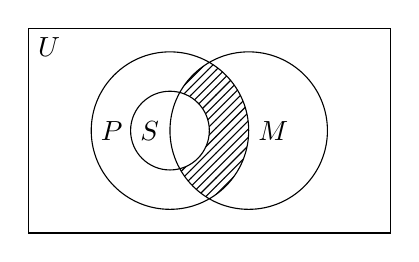
\begin{tikzpicture}
        \begin{scope}
            \clip (1,0) circle (1);
            \begin{scope}[even odd rule]
                \clip (0,0) circle (1) (0,0) circle (0.5);
                \filldraw [pattern = {north east lines}] (-2,-2) rectangle (2,2);
            \end{scope}
        \end{scope}
        \draw (0,0) circle (1) (1,0) circle (1) (0,0) circle (0.5);
        \draw (-1.8,-1.3) rectangle (2.8,1.3);
        \draw (-1.8,1.3) node [below right] {$U$} (-1,0) node [right] {$P$} (-0.5,0) node [right] {$S$} (1,0) node [right] {$M$};
    \end{tikzpicture}
\end{center}


关联目标:

暂未关联目标

答案: 暂无答案

解答或提示: 暂无解答与提示

使用记录:

暂无使用记录


出处: 2022届高三第一轮复习讲义
\item { (002711)}设集合$A=\{5,\log_2(a+3)\}$, $B=\{a,b\}$, 若$A\cap B=\{2\}$, 则$A\cup B=$\blank{50}.


关联目标:

暂未关联目标

答案: 暂无答案

解答或提示: 暂无解答与提示

使用记录:

暂无使用记录


出处: 2022届高三第一轮复习讲义
\item { (002712)}设集合$A\cap \{-2,0,1\}=\{0,1\}$, $A\cup \{-2,0,2\}=\{-2,0,1,2\}$, 则满足上述条件的集合$A$的个数为\blank{50}个.


关联目标:

暂未关联目标

答案: 暂无答案

解答或提示: 暂无解答与提示

使用记录:

暂无使用记录


出处: 2022届高三第一轮复习讲义
\item { (002713)}若集合$A=\{x|x\le 2\}$, $B=\{x|x\ge a\}$, 满足$A\cap B=\{2\}$, 则实数$a=$\blank{50}.


关联目标:

暂未关联目标

答案: 暂无答案

解答或提示: 暂无解答与提示

使用记录:

暂无使用记录


出处: 2022届高三第一轮复习讲义
\item { (002714)}若集合$M=[a-1,a+1]$, $N=(-\infty,-1)\cup [2,+\infty)$, 且$M\cap N=\varnothing$, 则实数$a$的取值范围为\blank{50}.


关联目标:

暂未关联目标

答案: 暂无答案

解答或提示: 暂无解答与提示

使用记录:

暂无使用记录


出处: 2022届高三第一轮复习讲义
\item { (002715)}集合$A=\{(x,y)|x^2+y^2=25\}$, $B=\{(x,y)|x=3y=4\}$, 则$A\cap B$的子集个数是\blank{50}个.


关联目标:

暂未关联目标

答案: 暂无答案

解答或提示: 暂无解答与提示

使用记录:

暂无使用记录


出处: 2022届高三第一轮复习讲义
\item { (002716)}已知集合$M=\{x|x=3m+1, \ m\in \mathbf{Z}\}$, $N=\{y|y=3m+2, \ m\in \mathbf{Z}\}$, 若$x_0\in M$, $y_0\in N$, 则$x_0y_0$与集合$M,N$的关系是\bracket{20}.
\twoch{$x_0y_0\in M$但$x_0y_0$$\notin N$}{$x_0y_0\in N$但$x_0y_0\notin M$}{$x_0y_0\notin M$且$x_0y_0\notin N$}{$x_0y_0$$\in M$且$x_0y_0\in N$}


关联目标:

暂未关联目标

答案: 暂无答案

解答或提示: 暂无解答与提示

使用记录:

暂无使用记录


出处: 2022届高三第一轮复习讲义
\item { (002718)}设常数$a\in \mathbf{R}$, 集合$A=\{x|\dfrac{3-2x}{x-1}+1 \ge 0, \ x\in \mathbf{R}\}$, $B=\{x|2ax<a+x, \ x\in \mathbf{R} \}$.若$A\cup B=B$, 求$a$的取值范围.


关联目标:

暂未关联目标

答案: 暂无答案

解答或提示: 暂无解答与提示

使用记录:

暂无使用记录


出处: 2022届高三第一轮复习讲义
\item { (002720)}设常数$k\in \mathbf{R}$, 关于$x$的不等式组$\begin{cases} x^2-x-2>0, \\ 2x^2+(2k+5)x+5k<0 \end{cases}$ 整数解的集合为$\{-2\}$, 求实数$k$的取值范围.


关联目标:

暂未关联目标

答案: 暂无答案

解答或提示: 暂无解答与提示

使用记录:

暂无使用记录


出处: 2022届高三第一轮复习讲义
\item { (002723)}定义集合运算: $A\odot B=\{z|z=xy(x+y), \ x\in A, \ y\in B \}$, 设集合$A=\{0,1\}$, $B=\{2,3\}$, 则集合$A\odot B$的所有元素之和为\blank{50}.


关联目标:

暂未关联目标

答案: 暂无答案

解答或提示: 暂无解答与提示

使用记录:

暂无使用记录


出处: 2022届高三第一轮复习讲义
\item { (002725)}集合$A=\{(x,y)|y=|x|+1\}$, $B=\{(x,y)|y=\dfrac12x+a\}$, 若$A\cap B=\varnothing$, 则$a$的取值范围是\blank{50}.


关联目标:

暂未关联目标

答案: 暂无答案

解答或提示: 暂无解答与提示

使用记录:

暂无使用记录


出处: 2022届高三第一轮复习讲义
\item { (002727)}已知集合$A=\{x|ax^2-3x+2=0\}$至多有一个元素, 则$a$的取值范围是\blank{50}; 若至少有一个元素, 则$a$的取值范围是\blank{50}.


关联目标:

暂未关联目标

答案: 暂无答案

解答或提示: 暂无解答与提示

使用记录:

暂无使用记录


出处: 2022届高三第一轮复习讲义
\item { (002728)}设含有三个实数的集合既可以表示为$\{a,\dfrac ba,1\}$, 又可以表示为$\{a^2,a+b,0\}$, 那么$a+b=$\blank{50}.


关联目标:

暂未关联目标

答案: 暂无答案

解答或提示: 暂无解答与提示

使用记录:

暂无使用记录


出处: 2022届高三第一轮复习讲义
\item { (002729)}设$f(x)=x^2-12x+36$, $A=\{a|1\le a\le 10, \ a\in \mathbf{N}\}$, $B=\{b|b=f(a),\ a\in A\}$, 又设$C=A\cap B$. 求集合$C$.


关联目标:

暂未关联目标

答案: 暂无答案

解答或提示: 暂无解答与提示

使用记录:

暂无使用记录


出处: 2022届高三第一轮复习讲义
\item { (002731)}填写下列命题的否定形式:\\
(1) $m\le 0$或$n>0$: \blank{200};\\
(2) 空间三条直线$l,m,n$两两相交: \blank{200};\\
(3) 复数$z_1,z_2,z_3$中至多一个为纯虚数: \blank{200}.


关联目标:

暂未关联目标

答案: 暂无答案

解答或提示: 暂无解答与提示

使用记录:

暂无使用记录


出处: 2022届高三第一轮复习讲义
\item { (002732)}已知$a,b$是整数, 写出命题``若$ab$为偶数, 则$a+b$为偶数''的逆命题、否命题、逆否命题, 并判断所写命题的真假.\\
逆命题:\blank{200}, 真假: \blank{20};\\
否命题:\blank{200}, 真假: \blank{20};\\
逆否命题:\blank{200}, 真假: \blank{20}.


关联目标:

暂未关联目标

答案: 暂无答案

解答或提示: 暂无解答与提示

使用记录:

暂无使用记录


出处: 2022届高三第一轮复习讲义
\item { (002735)}下列各组命题中互为等价命题的是\bracket{20}.
\twoch{$A\subseteq B$与$A\cup B=B$}{$x\in A$且$x\in B$与$x\in A\cup B$}{$a\in A\cap B$与$a\in A$或$a\in B$}{$m\in A\cap B$与$m\in A\cup B$}


关联目标:

暂未关联目标

答案: 暂无答案

解答或提示: 暂无解答与提示

使用记录:

暂无使用记录


出处: 2022届高三第一轮复习讲义
\item { (002741)}已知关于$x$的实系数二次方程$a x^2 +bx+c=0\ (a>0)$, 分别求下列命题的一个充要条件:\\
(1) 方程有一正根, 一根是零;\\
(2) 两根都比$2$小.


关联目标:

暂未关联目标

答案: 暂无答案

解答或提示: 暂无解答与提示

使用记录:

暂无使用记录


出处: 2022届高三第一轮复习讲义
\item { (002742)}设$a,b\in \mathbf{R}$, 写出命题``若$a+b>0$且$ab>0$, 则$a>0$且$b>0$''的逆否命题.


关联目标:

暂未关联目标

答案: 暂无答案

解答或提示: 暂无解答与提示

使用记录:

暂无使用记录


出处: 2022届高三第一轮复习讲义
\item { (002744)}已知$x,y\in \mathbf{R}$, 有如下四个命题: \textcircled{1} $x^2+y^2<1$; \textcircled{2} $|x|+|y|<1$; \textcircled{3} $|x|<1$且$y|<1$; \textcircled{4} $|x+y|<1$. 则\blank{50}是\blank{50}的充分非必要条件(答案可能不唯一).


关联目标:

暂未关联目标

答案: 暂无答案

解答或提示: 暂无解答与提示

使用记录:

暂无使用记录


出处: 2022届高三第一轮复习讲义
\item { (002747)}命题甲: 关于$x$的方程$x^2+x+m=0$有两个相异的负根; 命题乙: 关于$x$的方程$4x^2+x+m=0$无实根, 若这两个命题有且只有一个是真命题, 求实数$m$的取值范围.
*


关联目标:

暂未关联目标

答案: 暂无答案

解答或提示: 暂无解答与提示

使用记录:

暂无使用记录


出处: 2022届高三第一轮复习讲义
\item { (002750)}命题(1) $a>b\Rightarrow ac^2>bc^2$;   (2) $ac^2>bc^2\Rightarrow a>b$;     (3) $a>b\Rightarrow \dfrac 1a<\dfrac 1b$; (4) $a<b<0, \ c<d<0\Rightarrow ac>bd$;   (5) $\sqrt[n]a>\sqrt[n]b\Rightarrow a>b \ (n\in \mathbf{N}^*)$;    (6) $a+c<b+d\Leftrightarrow \begin{cases} a<b, \\ c<d; \end{cases}$ (7) $a<b<0\Rightarrow a^2>ab>b^2$. 其中真命题的序号是\blank{50}.


关联目标:

暂未关联目标

答案: 暂无答案

解答或提示: 暂无解答与提示

使用记录:

暂无使用记录


出处: 2022届高三第一轮复习讲义
\item { (002807)}已知关于$x$的不等式$\dfrac{ax-5}{x^2-a}<0$的解集为$M$.\\
(1) 当$a=5$时, 求集合$M$;\\
(2) 若$2\in M$且$5\notin M$, 求实数$a$的取值范围.


关联目标:

暂未关联目标

答案: 暂无答案

解答或提示: 暂无解答与提示

使用记录:

暂无使用记录


出处: 2022届高三第一轮复习讲义
\item { (002846)}设函数$y=f(x)$为定义在$\mathbf{R}$上的函数, 则命题: ``$f(-1)\ne f(1)$且$f(-1)\ne -f(1)$''是命题``$y=f(x)$既不是奇函数也不是偶函数''的\blank{50}条件(填``充分不必要''、``必要不充分''、``充要''、``既不充分也不必要''之中一个).


关联目标:

暂未关联目标

答案: 暂无答案

解答或提示: 暂无解答与提示

使用记录:

暂无使用记录


出处: 2022届高三第一轮复习讲义
\item { (002883)}*设定义在$\mathbf{R}$上的函数$y=f(x)$的满足: 对于任意$x\in \mathbf{R}$, 恒有$f(-x+1)=-f(x+1)$且$f(-x-1)=-f(x-1)$. 则下面命题中, 正确的命题的序号是\blank{50}.\\
\textcircled{1} 函数$y=f(x)$是偶函数; \textcircled{2} $2$是$y=f(x)$的周期; \textcircled{3} 函数$y=f(x)$图像关于$(1,0)$对称; \textcircled{4} 函数$y=f(x)$图像关于$(3,0)$对称.


关联目标:

暂未关联目标

答案: 暂无答案

解答或提示: 暂无解答与提示

使用记录:

暂无使用记录


出处: 2022届高三第一轮复习讲义
\item { (002891)}若函数$y=f(x)$, $y=g(x)$均为$\mathbf{R}$上增函数, 则下列命题中, 正确的命题的序号是\blank{50}.\\
\textcircled{1} $y=f(x)+g(x)$为增函数; \textcircled{2} $y=f(x)\cdot g(x)$为增函数; \textcircled{3} $y=f(g(x))$为增函数.


关联目标:

暂未关联目标

答案: 暂无答案

解答或提示: 暂无解答与提示

使用记录:

暂无使用记录


出处: 2022届高三第一轮复习讲义
\item { (002902)}*设$f(x)$、$g(x)$、$h(x)$是定义域为$R$的三个函数, 对于下列命题:\\
\textcircled{1} 若$f(x)+g(x)$、$f(x)+h(x)$、$g(x)+h(x)$均为增函数, 则$f(x)$、$g(x)$、$h(x)$中至少有一个是增函数;\\
\textcircled{2} 若$f(x)+g(x)$、$f(x)+h(x)$、$g(x)+h(x)$均是以$T$为周期的函数, 则$f(x)$、$g(x)$、$h(x)$均是以$T$为周期的函数, 下列判断正确的是\bracket{20}.
\twoch{\textcircled{1}和\textcircled{2}均为真命题}{\textcircled{1}和\textcircled{2}均为假命题}{\textcircled{1}为真命题, \textcircled{2}为假命题}{\textcircled{1}为假命题, \textcircled{2}为真命题}


关联目标:

暂未关联目标

答案: 暂无答案

解答或提示: 暂无解答与提示

使用记录:

暂无使用记录


出处: 2022届高三第一轮复习讲义
\item { (002908)}下列命题中, 正确的命题的序号是\blank{50}.\\
\textcircled{1} 当$\alpha =0$时, 函数$y={x^{\alpha }}$的图像是一条直线;\\
\textcircled{2} 幂函数的图像都经过(0, 0)和(1, 1)点;\\
\textcircled{3} 当$\alpha <0$且$y={x^{\alpha }}$是奇函数时, 它也是减函数;\\
\textcircled{4} 第四象限不可能有幂函数的图像.


关联目标:

暂未关联目标

答案: 暂无答案

解答或提示: 暂无解答与提示

使用记录:

暂无使用记录


出处: 2022届高三第一轮复习讲义
\item { (002913)}若集合$A=\{y|y={x^{\frac 13}}, \ -1\le x\le 1\}$, $B=\{y|y={x^{-\frac 12}}\}$, 则$A\cap B$等于\bracket{20}.
\fourch{$(0,1]$}{$[-1,1]$}{$\{1\}$}{$\{0,1\}$}


关联目标:

暂未关联目标

答案: 暂无答案

解答或提示: 暂无解答与提示

使用记录:

暂无使用记录


出处: 2022届高三第一轮复习讲义
\item { (002924)}设$y=f(x)$与$y=g(x)$是两个不同的幂函数, 集合$M=\{x|f(x)=g(x)  \}$, 则集合$M$中的元素是\bracket{20}.
\fourch{$1$或$2$}{$1$或$3$}{$1$或$2$或$3$}{$1$或$2$或$3$或$4$}


关联目标:

暂未关联目标

答案: 暂无答案

解答或提示: 暂无解答与提示

使用记录:

暂无使用记录


出处: 2022届高三第一轮复习讲义
\item { (002935)}若命题``函数$y=x+\dfrac ax$在区间$[1,2]$上存在反函数''为真命题, 则在下列值中, 能作为实数$a$的值的序号是\blank{50}.\\
\textcircled{1} $a=-1$; \textcircled{2} $a=1$; \textcircled{3} $a=\sqrt 2$; \textcircled{4} $a=\sqrt 5$.


关联目标:

暂未关联目标

答案: 暂无答案

解答或提示: 暂无解答与提示

使用记录:

暂无使用记录


出处: 2022届高三第一轮复习讲义
\item { (002956)}若集合$A=\{y|y=2\cdot (\dfrac 13)^{|x|}\}$, $B=\{ a|\log_a(3a-1)>0\}$, 则$A\cap B$=\blank{50}.


关联目标:

暂未关联目标

答案: 暂无答案

解答或提示: 暂无解答与提示

使用记录:

暂无使用记录


出处: 2022届高三第一轮复习讲义
\item { (002970)}*已知函数$f(x)=1+a\cdot (\dfrac 12)^x+(\dfrac 14)^x$.\\
(1) 当$a=1$时, 求函数$y=f(x)$在$(-\infty,0)$上的值域;\\
(2) 对于定义在集合$D$上的函数$y=f(x)$, 如果存在常数$M>0$, 满足: 对任意$x\in D$, 都有$|f(x)|\le M$成立, 则称$f(x)$是$D$上的有界函数, 其中$M$称为函数$f(x)$的一个上界.若函数$y=f(x)$在$[0,+\infty)$上是以$3$为一个上界的有界函数, 求实数$a$的取值范围.


关联目标:

暂未关联目标

答案: 暂无答案

解答或提示: 暂无解答与提示

使用记录:

暂无使用记录


出处: 2022届高三第一轮复习讲义
\item { (003064)}在单位圆中分别画出适合下列条件的角$\alpha$的终边的范围, 并写出角$\alpha$的集合.\\
(1) $\sin\alpha\ge \dfrac{\sqrt 3}2$;\\
(2) $\cos\alpha\le -\dfrac 12$;\\
(3) $\tan\alpha<-1$.


关联目标:

暂未关联目标

答案: 暂无答案

解答或提示: 暂无解答与提示

使用记录:

暂无使用记录


出处: 2022届高三第一轮复习讲义
\item { (003065)}与$-45^\circ$角终边相同的角的集合是\blank{50}.


关联目标:

暂未关联目标

答案: 暂无答案

解答或提示: 暂无解答与提示

使用记录:

暂无使用记录


出处: 2022届高三第一轮复习讲义
\item { (003068)}若$\sin\alpha\cdot\cos\alpha>0$, 则$\alpha$的值的集合是\blank{50}.


关联目标:

暂未关联目标

答案: 暂无答案

解答或提示: 暂无解答与提示

使用记录:

暂无使用记录


出处: 2022届高三第一轮复习讲义
\item { (003069)}若角$\alpha$的终边不在坐标轴上, $\sin\dfrac{\alpha}2>0$, $\cos\dfrac{\alpha}2<0$ , 则关于角$\alpha$, 以下命题正确的有\blank{50}(填序号).\\
\textcircled{1} 不在第一象限; \textcircled{2} 不在第二象限; \textcircled{3} 不在第三象限; \textcircled{4} 不在第四象限.


关联目标:

暂未关联目标

答案: 暂无答案

解答或提示: 暂无解答与提示

使用记录:

暂无使用记录


出处: 2022届高三第一轮复习讲义
\item { (003116)}下列命题中, 是$\tan\dfrac{\alpha}2=m$的充要条件的是\blank{50}(填序号).\\
\textcircled{1} $\dfrac{1-\cos \alpha}{\sin \alpha}$有意义且值为$m$; 	\textcircled{2} $\dfrac{\sin \alpha}{1+\cos \alpha}$有意义且值为$m$; \textcircled{3} $\sin \alpha =\dfrac{2m}{1+{m^2}}$.


关联目标:

暂未关联目标

答案: 暂无答案

解答或提示: 暂无解答与提示

使用记录:

暂无使用记录


出处: 2022届高三第一轮复习讲义
\item { (003133)}在三角形$ABC$中, $\tan A\tan B>1$, 则以下命题正确的是\blank{50}(填序号).\\
\textcircled{1} 三角形$ABC$一定是锐角三角形;
\textcircled{2} 三角形$ABC$可能是钝角三角形;
\textcircled{3} 三角形$ABC$可能是直角三角形.


关联目标:

暂未关联目标

答案: 暂无答案

解答或提示: 暂无解答与提示

使用记录:

暂无使用记录


出处: 2022届高三第一轮复习讲义
\item { (003154)}已知$T>0$. 下列命题中, 能成为命题``函数$f(x)$的一个周期为$T$''的必要不充分条件的是\bracket{20}.
\twoch{函数$f(x)$的一个周期是$-T$}{函数$f(x)$的一个周期是$2T$}{函数$f(x)$的一个周期是$\dfrac T2$}{函数$f(x)$存在最小正周期}


关联目标:

暂未关联目标

答案: 暂无答案

解答或提示: 暂无解答与提示

使用记录:

暂无使用记录


出处: 2022届高三第一轮复习讲义
\item { (003235)}等差数列$\{a_n\}$中, $S_n$为前$n$项和, 且$S_6<S_7$,$S_7>S_8$, 给出下列命题:\\
(1) 数列$\{a_n\}$中前$7$项是递增的, 从第$8$项开始递减;
(2) $S_9$一定小于$S_6$;
(3) $a_1$是$\{a_n\}$各项中的最大的;
(4) $S_7$不一定是$\{S_n\}$中最大项. 其中正确的序号是\blank{50}.


关联目标:

暂未关联目标

答案: 暂无答案

解答或提示: 暂无解答与提示

使用记录:

暂无使用记录


出处: 2022届高三第一轮复习讲义
\item { (003275)}用数学归纳法证明``对于任意正偶数$n$, $a^n-b^n$能被$a+b$整除''时, 其第二步论证应该是\bracket{20}.
\onech{假设$n=k$, $k\in \mathbf{N}^*$时命题成立, 证明$n=k+1$时, 命题也成立}{假设$n=2k$, $k\in \mathbf{N}^*$时命题成立, 证明$n=2k+1$时, 命题也成立}{假设$n=k$, $k\in \mathbf{N}^*$时命题成立, 证明$n=k+2$时, 命题也成立}{假设$n=2k$, $k\in \mathbf{N}^*$时命题成立, 证明$n=2k+2$时, 命题也成立}


关联目标:

暂未关联目标

答案: 暂无答案

解答或提示: 暂无解答与提示

使用记录:

暂无使用记录


出处: 2022届高三第一轮复习讲义
\item { (003327)}已知$\overrightarrow a$、$\overrightarrow b$、$\overrightarrow c$为非零向量, 下列命题中假命题是\blank{50}.\\
(1) $\overrightarrow a+(-\overrightarrow a)=0$;\\
(2) 若$| \overrightarrow a|=|\overrightarrow b|$, 则$\overrightarrow a=\overrightarrow b$或$\overrightarrow a=-\overrightarrow b$;\\
(3) $\overrightarrow a\parallel \overrightarrow b$是$| \overrightarrow a+\overrightarrow b|=|\overrightarrow a|+|\overrightarrow b|$成立的充分非必要条件;\\
(4) $\overrightarrow a+\overrightarrow b+\overrightarrow c=\overrightarrow 0$是$\overrightarrow a$、$\overrightarrow b$、$\overrightarrow c$可以首尾相接构成三角形的必要非充分条件.


关联目标:

暂未关联目标

答案: 暂无答案

解答或提示: 暂无解答与提示

使用记录:

暂无使用记录


出处: 2022届高三第一轮复习讲义
\item { (003354)}给出下列命题:\\
\textcircled{1} 非零向量$\overrightarrow a$、$\overrightarrow b$满足$|\overrightarrow a|=|\overrightarrow b|=|\overrightarrow a-\overrightarrow b|$, 则$\overrightarrow a$与$\overrightarrow a+\overrightarrow b$的夹角为$30^\circ$;\\
\textcircled{2} $\overrightarrow b\cdot \overrightarrow b>0$, 是$\overrightarrow a$、$\overrightarrow b$的夹角为锐角的充要条件;\\
\textcircled{3}  将函数$y=|x-1|$的图像按向量$\overrightarrow a=(-1,0)$平移, 得到的图像对应的函数表达式为$y=|x|$;\\
\textcircled{4} 在$\triangle ABC$中, 若$(\overrightarrow{AB}+\overrightarrow{AC})\cdot (\overrightarrow{AB}-\overrightarrow{AC})=0$, 则$\triangle ABC$为等腰三角形.\\
以上命题正确的是\blank{50}(注: 把你认为正确的命题的序号都填上).


关联目标:

暂未关联目标

答案: 暂无答案

解答或提示: 暂无解答与提示

使用记录:

暂无使用记录


出处: 2022届高三第一轮复习讲义
\item { (003380)}如图, 用$35$个单位正方形拼成一个矩形, 点$P_1$、$P_2$、$P_3$、$P_4$以及四个标记为``
\begin{tikzpicture} \filldraw ({-0.0625*sqrt(3)},-0.0625) -- ({0.0625*sqrt(3)},-0.0625) -- (0,0.125) -- cycle; \end{tikzpicture}''的点在正方形的顶点处, 设集合$\Omega =\{P_1,P_2,P_3,P_4\}$, 点$P\in \Omega$, 过$P$作直线$l_P$, 使得不在$l_P$上的``
\begin{tikzpicture} \filldraw ({-0.0625*sqrt(3)},-0.0625) -- ({0.0625*sqrt(3)},-0.0625) -- (0,0.125) -- cycle; \end{tikzpicture}''的点分布在$l_P$的两侧. 用$D_1(l_P)$和$D_2(l_P)$分别表示$l_P$一侧和另一侧的``
\begin{tikzpicture} \filldraw ({-0.0625*sqrt(3)},-0.0625) -- ({0.0625*sqrt(3)},-0.0625) -- (0,0.125) -- cycle; \end{tikzpicture}''的点到$l_P$的距离之和. 若过$P$的直线$l_P$中有且只有一条满足$D_1(l_P)=D_2(l_P)$, 则$\Omega$中所有这样的$P$为\blank{50}.
\begin{center}
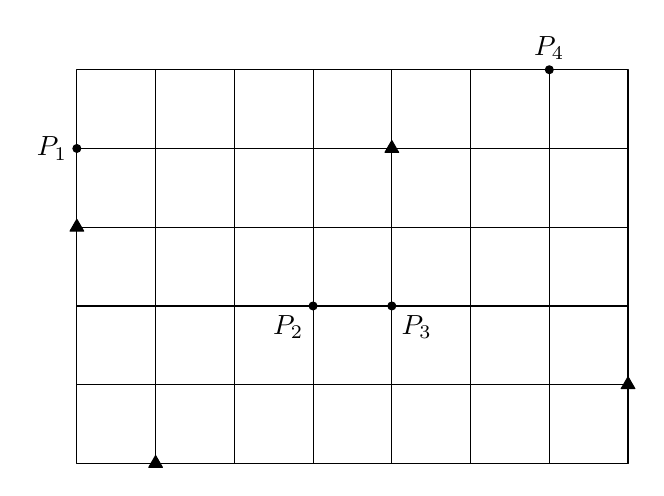
\begin{tikzpicture}[>=latex, line cap = round, line join = round]
    \foreach \i in {0,1,...,7}
        \draw (\i,0) -- (\i,5);
    \foreach \i in {0,1,...,5}
        \draw (0,\i) -- (7,\i);
    \filldraw (0,4) circle (0.05) node [left] {$P_1$};
    \filldraw (3,2) circle (0.05) node [below left] {$P_2$};
    \filldraw (4,2) circle (0.05) node [below right] {$P_3$};
    \filldraw (6,5) circle (0.05) node [above] {$P_4$};
    \filldraw (1,0) ++ (210:0.1) --++ ({0.1*sqrt(3)},0) --++ (120:{0.1*sqrt(3)}) -- cycle;
    \filldraw (0,3) ++ (210:0.1) --++ ({0.1*sqrt(3)},0) --++ (120:{0.1*sqrt(3)}) -- cycle;
    \filldraw (4,4) ++ (210:0.1) --++ ({0.1*sqrt(3)},0) --++ (120:{0.1*sqrt(3)}) -- cycle;
    \filldraw (7,1) ++ (210:0.1) --++ ({0.1*sqrt(3)},0) --++ (120:{0.1*sqrt(3)}) -- cycle;
\end{tikzpicture}
\end{center}


关联目标:

暂未关联目标

答案: 暂无答案

解答或提示: 暂无解答与提示

使用记录:

暂无使用记录


出处: 2022届高三第一轮复习讲义
\item { (003452)}下列命题中, 假命题有\blank{50}(填入序号).\\
(1) 平行于同一平面的两直线平行; (2) 平行于同一直线的两平面平行; (3) 平行于同一直线的两直线平行; (4) 平行于同一平面的两平面平行.


关联目标:

暂未关联目标

答案: 暂无答案

解答或提示: 暂无解答与提示

使用记录:

暂无使用记录


出处: 2022届高三第一轮复习讲义
\item { (003466)}对于分别与两条异面直线都相交的两条直线, 下列结论中, 真命题有\blank{50}(填入序号).\\
(1) 一定是异面直线; (2) 不可能是平行直线; (3) 不可能是相交直线.


关联目标:

暂未关联目标

答案: 暂无答案

解答或提示: 暂无解答与提示

使用记录:

暂无使用记录


出处: 2022届高三第一轮复习讲义
\item { (003470)}下列命题中, 假命题有\blank{50}(填入序号).\\
(1) 底面是正多边形的棱锥是正棱锥; (2) 侧棱都相等的棱锥是正棱锥; (3) 有两个侧面是矩形的棱柱是直棱柱.


关联目标:

暂未关联目标

答案: 暂无答案

解答或提示: 暂无解答与提示

使用记录:

暂无使用记录


出处: 2022届高三第一轮复习讲义
\item { (003484)}下列命题中, 假命题有\blank{50}(填入序号).\\
(1) 经过球上任意两点, 能且仅能作一个大圆;\\
(2) 与球的一条直径垂直的大圆有且只有一个;\\
(3) 球的表面积是它大圆面积的$4$倍;\\
(4) 如果过球面上两点可以作小圆, 那么``小圆的劣弧长''大于``过这两点的大圆的劣弧长''.


关联目标:

暂未关联目标

答案: 暂无答案

解答或提示: 暂无解答与提示

使用记录:

暂无使用记录


出处: 2022届高三第一轮复习讲义
\item { (003501)}用``$\subseteq$''连接集合$\mathbf{Z}$、$\mathbf{Q}$、$\mathbf{R}$、$\mathbf{C}$:\blank{50}.


关联目标:

暂未关联目标

答案: 暂无答案

解答或提示: 暂无解答与提示

使用记录:

暂无使用记录


出处: 2022届高三第一轮复习讲义
\item { (003508)}判断下列命题的真假, 对于假命题请至少举一个反例.
\begin{center}
    \begin{tabular}{|c|c|p{.25\textwidth}<{\centering}|}
        \hline
        命题 & 填``真''或``假'' & 反例\\ \hline
        (1) 复数$z$是实数的充要条件是$z-\overline z=0$.	& & \\ \hline
        (2) 复数$z$是纯虚数的充要条件是$z+\overline z=0$. & & \\ \hline
        (3) $z+\overline{z}$和$z\cdot \overline{z}$都是实数. & & \\ \hline
        (4) 已知$|z|=2$, 那么$z=\pm 2$或$\pm 2\mathrm{i}$. & & \\ \hline
    \end{tabular}
\end{center}


关联目标:

暂未关联目标

答案: 暂无答案

解答或提示: 暂无解答与提示

使用记录:

暂无使用记录


出处: 2022届高三第一轮复习讲义
\item { (003516)}下列命题中正确的有:\blank{50}.\\
(1) 设$z_1,z_2$为复数, 若$z_1^2+z_2^2=0$, 则$z_1+z_2=0$;\\
(2) 设$z_1,z_2$为复数, $z_1\cdot z_2=0$的充要条件为$z_1=0$或$z_2=0$;\\
(3) 若$z_1+z_2>0$, 那么$z_1>-z_2$;\\
(4) 若$|z|\le 1$, 则$-1\le z\le 1$;\\
(5) 若$z\in \mathbf{C}$, 那么$|z^2|=|z|^2$;\\
(6) 若$z\in \mathbf{C}$, 那么$|z|=\sqrt{z^2}$.


关联目标:

暂未关联目标

答案: 暂无答案

解答或提示: 暂无解答与提示

使用记录:

暂无使用记录


出处: 2022届高三第一轮复习讲义
\item { (003533)}若集合$A=\{z||z+5\mathrm{i}|-|z-5\mathrm{i}|=8\}$, $B=\{z||z|=4\}$, 则$A\cap B=$\blank{50}.


关联目标:

暂未关联目标

答案: 暂无答案

解答或提示: 暂无解答与提示

使用记录:

暂无使用记录


出处: 2022届高三第一轮复习讲义
\item { (003542)}已知关于$x$的实系数一元二次方程$ax^2+bx+c=0\ (a\ne 0)$在复数集中的两个根为$\alpha,\beta$, 下列命题中正确的有\blank{50}.\\
\textcircled{1} $\alpha$和$\beta$互为共轭复数;\\
\textcircled{2} $\alpha +\beta =-\dfrac ba$, $\alpha \beta =\dfrac ca$;\\
\textcircled{3} $\alpha$和$\beta$分别为$\dfrac{-b\pm \sqrt{b^2}-4ac}{2a}$;\\
\textcircled{4} $|\alpha -\beta|^2=(\alpha-\beta)^2$;\\
\textcircled{5} $ax^2+bx+c=a(x-\alpha)(x-\beta)$.


关联目标:

暂未关联目标

答案: 暂无答案

解答或提示: 暂无解答与提示

使用记录:

暂无使用记录


出处: 2022届高三第一轮复习讲义
\item { (003610)}已知集合$A=\{1,2,4\}$,$B=\{2,4,5\}$, 则$A\cap B=$\blank{50}.


关联目标:

暂未关联目标

答案: 暂无答案

解答或提示: 暂无解答与提示

使用记录:

暂无使用记录


出处: 上海2020年秋季高考试题1
\item { (003625)}命题$p$: 存在$a\in \mathbf{R}$且$a\ne 0$, 对任意的$x\in \mathbf{R}$, 均有$f(x+a)<f(x)+f(a)$恒成立. 已知命题$q_1$: $f(x)$单调递减, 且$f(x)>0$恒成立; 命题$q_2$: $f(x)$单调递增, 且存在${x_0}<0$使得$f({x_0})=0$. 则下列说法正确的是\bracket{20}.
\twoch{$q_1$、$q_2$都是$p$的充分条件}{只有$q_1$是$p$的充分条件}{只有$q_2$是$p$的充分条件}{$q_1$、$q_2$都不是$p$的充分条件}


关联目标:

暂未关联目标

答案: 暂无答案

解答或提示: 暂无解答与提示

使用记录:

20220630	2022届高三1班	\fcolorbox[rgb]{0,0,0}{1.000,0.466,0}{0.767}


出处: 上海2020年秋季高考试题16
\item { (003631)}已知集合$A=(-\infty,3)$, $B=(2,+\infty)$, 则$A\cap B=$\blank{50}.


关联目标:

暂未关联目标

答案: 暂无答案

解答或提示: 暂无解答与提示

使用记录:

暂无使用记录


出处: 上海2019年秋季高考试题1
\item { (003672)}给定无穷数列$\{a_n\}$, 若无穷数列$\{b_n\}$满足: 对任意$n\in \mathbf{N}^*$, 都有$|b_n-a_n|\le 1$, 则称$\{b_n\}$与$\{a_n\}$``接近''.\\
(1) 设$\{a_n\}$是首项为$1$, 公比为$\dfrac{1}{2}$的等比数列, $b_n=a_{n+1}+1, \ n\in \mathbf{N}^*$. 判断数列$\{b_n\}$是否与$\{a_n\}$接近, 并说明理由;\\
(2) 设数列$\{a_n\}$的前四项为: $a_1=1$, $a_2=2$, $a_3=4$, $a_4=8$, $\{b_n\}$是一个与$\{a_n\}$接近的数列, 记集合$M=\{x|x=b_i, \ i=1,2,3,4\}$, 求$M$中元素的个数$m$;\\
(3) 已知$\{a_n\}$是公差为$d$的等差数列. 若存在数列$\{b_n\}$满足: $\{b_n\}$与$\{a_n\}$接近, 且在$b_2-b_1,b_3-b_2,\cdots,b_{201}-b_{200}$中至少有$100$个为正数, 求$d$的取值范围.


关联目标:

暂未关联目标

答案: 暂无答案

解答或提示: 暂无解答与提示

使用记录:

暂无使用记录


出处: 上海2018年秋季高考试题21
\item { (003673)}已知集合$A=\{1,2,3,4\}$, $B=\{3,4,5\}$, 则$A\cap B=$\blank{50}.


关联目标:

暂未关联目标

答案: 暂无答案

解答或提示: 暂无解答与提示

使用记录:

暂无使用记录


出处: 上海2017年秋季高考试题1
\item { (003684)}如图, 用$35$个单位正方形拼成一个矩形, 点$P_1,P_2,P_3,P_4$以及四个标记为``
\begin{tikzpicture}
\filldraw ({-0.0625*sqrt(3)},-0.0625) -- ({0.0625*sqrt(3)},-0.0625) -- (0,0.125) -- cycle;
\end{tikzpicture}''的点在正方形的顶点处, 设集合$\Omega=\{P_1,P_2,P_3,P_4\}$, 点$P\in \Omega$. 过$P$作直线$l_P$, 使得不在$l_P$上的``
\begin{tikzpicture}
\filldraw ({-0.0625*sqrt(3)},-0.0625) -- ({0.0625*sqrt(3)},-0.0625) -- (0,0.125) -- cycle;
\end{tikzpicture}''的点分布在$l_P$的两侧. 用$D_1(l_P)$和$D_2(l_P)$分别表示$l_P$一侧和另一侧的``
\begin{tikzpicture}
\filldraw ({-0.0625*sqrt(3)},-0.0625) -- ({0.0625*sqrt(3)},-0.0625) -- (0,0.125) -- cycle;
\end{tikzpicture}''的点到$l_P$的距离之和. 若过$P$的直线$l_P$中有且只有一条满足$D_1(l_P)=D_2(l_P)$, 则$\Omega$中所有这样的$P$为\blank{50}.
\begin{center}
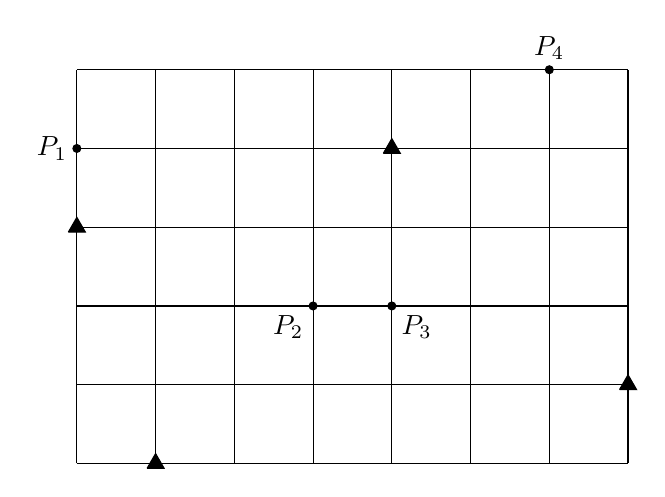
\begin{tikzpicture}
\foreach \i in {0,1,2,3,4,5,6,7}{\draw (\i,0) -- (\i,5);};
\foreach \i in {0,1,2,3,4,5}{\draw (0,\i) -- (7,\i);};
\filldraw  (1,0) ++ ({-0.0625*sqrt(3)},-0.0625) coordinate(P) --++ ({2*0.0625*sqrt(3)},0) --++ ({-0.0625*sqrt(3)},{3*0.0625}) -- (P);
\filldraw  (7,1) ++ ({-0.0625*sqrt(3)},-0.0625) coordinate(P) --++ ({2*0.0625*sqrt(3)},0) --++ ({-0.0625*sqrt(3)},{3*0.0625}) -- (P);
\filldraw  (0,3) ++ ({-0.0625*sqrt(3)},-0.0625) coordinate(P) --++ ({2*0.0625*sqrt(3)},0) --++ ({-0.0625*sqrt(3)},{3*0.0625}) -- (P);
\filldraw  (4,4) ++ ({-0.0625*sqrt(3)},-0.0625) coordinate(P) --++ ({2*0.0625*sqrt(3)},0) --++ ({-0.0625*sqrt(3)},{3*0.0625}) -- (P);
\filldraw (0,4) circle (0.05) node [left] {$P_1$};
\filldraw (3,2) circle (0.05) node [below left] {$P_2$};
\filldraw (4,2) circle (0.05) node [below right] {$P_3$};
\filldraw (6,5) circle (0.05) node [above] {$P_4$};
\end{tikzpicture}
\end{center}


关联目标:

暂未关联目标

答案: 暂无答案

解答或提示: 暂无解答与提示

使用记录:

暂无使用记录


出处: 上海2017年秋季高考试题12
\item { (003695)}设实数$a,b,c$满足: $ac\ne 0$且$a\ne c$, 集合$A=\{y|y=ax^2+bx+c, \ x\in \mathbf{R}\}$, $B=\{y|y=cx^2+bx+a\}$, 以下结论一定正确的是\bracket{20}.
\fourch{$A\subseteq B$}{$B\subseteq A$}{$A\cup B=\mathbf{R}$}{$A\cap B\ne\varnothing$}


关联目标:

暂未关联目标

答案: 暂无答案

解答或提示: 暂无解答与提示

使用记录:

暂无使用记录


出处: 2022届高三高考前冲刺题精选
\item { (003700)}已知$a,b$为空间两条互相垂直的直线, 等腰$\mathrm{Rt}\triangle ABC$的直角边$AC$所在直线与$a,b$都垂直, 斜边$AB$以直线$AC$为旋转轴旋转. 有下列结论: \textcircled{1} 当直线$AB$与$a$所成的角为$60^\circ$时, $AB$与$b$所成的角为$30^\circ$; \textcircled{2} 直线$AB$与$a$所成角的最小值为$45^\circ$; \textcircled{3} 直线$AB$与$a$所成角的最大值为$60^\circ$. 其中所有真命题的序号为\blank{50}.


关联目标:

暂未关联目标

答案: 暂无答案

解答或提示: 暂无解答与提示

使用记录:

暂无使用记录


出处: 2022届高三高考前冲刺题精选
\item { (003702)}设$\overrightarrow a,\overrightarrow b,\overrightarrow c$是平面上的向量,$|\overrightarrow a| =1,|\overrightarrow b| =3,|\overrightarrow c|=4$, 且$\overrightarrow b\cdot \overrightarrow c=0$, 实数$\lambda$满足$0 \le \lambda \le 1$. 若$\overrightarrow a,\overrightarrow b,\overrightarrow c$及$\lambda$, 使得$s=|\overrightarrow a-\lambda \overrightarrow b-(1-\lambda)\overrightarrow c|$是正整数, 则$s$的值的集合是\blank{50}.


关联目标:

暂未关联目标

答案: 暂无答案

解答或提示: 暂无解答与提示

使用记录:

暂无使用记录


出处: 2022届高三高考前冲刺题精选
\item { (003707)}若全集$U=\{x|x^2-7x+12\le 0\}$, 集合$M=\{x|3<x<4\}$, $N=\left\{x\left|\dfrac{x-3}{4-x}\ge 0\right.\right\}$, 则$\complement_U M\cap \complement_U N=$\blank{50}.


关联目标:

暂未关联目标

答案: 暂无答案

解答或提示: 暂无解答与提示

使用记录:

暂无使用记录


出处: 2016年双基百分百
\item { (003719)}若集合$A=\{x|x^2-2x<0\}$, $B=\{x||x|<1\}$, 则$A\cup B$等于\blank{50}.


关联目标:

暂未关联目标

答案: 暂无答案

解答或提示: 暂无解答与提示

使用记录:

暂无使用记录


出处: 2016年双基百分百
\item { (003727)}从集合$\{0,1,2,3\}$的所有非空子集中, 等可能地取出一个. 则取出的非空子集中所有元素之和恰为$5$的概率为\blank{50}.


关联目标:

暂未关联目标

答案: 暂无答案

解答或提示: 暂无解答与提示

使用记录:

暂无使用记录


出处: 2016年双基百分百
\item { (003745)}已知集合$A=\{y|y=\sin x, \ x\in \mathbf{R}\}$, $B=\{x|x(2-x)>0\}$, 则$A\cup B=$\blank{50}.


关联目标:

暂未关联目标

答案: 暂无答案

解答或提示: 暂无解答与提示

使用记录:

暂无使用记录


出处: 2016年双基百分百
\item { (003758)}已知$a\in\mathbf{R}$, 命题$P:$``实系数一元二次方程$x^2+ax+2=0$的两根都是虚数''; 命题$Q:$``存在复数$z$同时满足$|z|=2$且$|z+a|=1$''.
是判断命题$P$和命题$Q$之间是否存在推出关系? 说明你的理由.


关联目标:

暂未关联目标

答案: 暂无答案

解答或提示: 暂无解答与提示

使用记录:

暂无使用记录


出处: 2016年双基百分百
\item { (003760)}已知集合$A=\{1,3,\sqrt{m}\}$, $B=\{1,m\}$, $A\cup B=A$, 则$m=$\blank{50}.


关联目标:

暂未关联目标

答案: 暂无答案

解答或提示: 暂无解答与提示

使用记录:

暂无使用记录


出处: 2016年双基百分百
\item { (003774)}已知集合$A=\left\{x\left|\dfrac{2x+1}{x+2}<1, \ x\in \mathbf{R}\right.\right\}$, 函数$f(x)=|mx+1| \ (m\in \mathbf{R})$. 函数$g(x)=x^2+ax+b \ (a,b\in \mathbf{R})$的值域为$[0,+\infty)$.\\
(1) 若不等式$f(x)<3$的解集为$A$, 求$m$的值;\\
(2) 在(1)的条件下, 若$\left|f(x)-2f\left(\dfrac x 2\right)\right|\le k$恒成立, 求$k$的取值范围;\\
(3) 若关于$x$的不等式$g(x)<c$的解集为$(m,m+6)$, 求实数$c$的值.


关联目标:

暂未关联目标

答案: 暂无答案

解答或提示: 暂无解答与提示

使用记录:

暂无使用记录


出处: 2016年双基百分百
\item { (003776)}命题``已知$x,y\in \mathbf{R}$,  若$x+y>2$, 则$x>1$且$y>1$''的否命题是\blank{150}; 该否命题是\blank{50}命题(填``真'',``假'').


关联目标:

暂未关联目标

答案: 暂无答案

解答或提示: 暂无解答与提示

使用记录:

暂无使用记录


出处: 2016年双基百分百
\item { (003800)}下列命题中正确的是\blank{30}.
\twoch{若$ac>bc$, 则$a>b$}{若$a^2>b^2$, 则$a>b$}{若$\dfrac 1a>\dfrac 1b$, 则$a<b$}{若$\sqrt{a}<\sqrt{b}$, 则$a<b$}


关联目标:

暂未关联目标

答案: 暂无答案

解答或提示: 暂无解答与提示

使用记录:

暂无使用记录


出处: 2016年双基百分百
\item { (003805)}已知命题$p:$``若$\overrightarrow{a}=\overrightarrow{b}$, 则$|\overrightarrow{a}|=|\overrightarrow{b}|$'', 则命题$p$及其逆命题, 否命题, 逆否命题中, 正确命题的个数是\blank{50}.


关联目标:

暂未关联目标

答案: 暂无答案

解答或提示: 暂无解答与提示

使用记录:

暂无使用记录


出处: 2016年双基百分百
\item { (003813)}在数列$\{a_n\}$中, 若$a_n^2-a_{n+1}^2=p\ (n\ge 1, \ n\in\mathbf{N}^*, \ p$为常数$)$, 则称$\{a_n\}$为``等方差数列''. 下列是对``等方差数列''的判断,
\textcircled{1} 若$\{a_n\}$是等方差数列, 则$\{a_n^2\}$是等差数列;
\textcircled{2} $\{(-1)^n\}$是等方差数列;
\textcircled{3} 若$\{a_n\}$是等方差数列, 则$\{a_{kn}\} \ (k\in \mathbf{N}^*, \ k$为常数$)$也是等方差数列.
其中真命题的序号为\blank{50}(将所有真命题的序号填写在横线上).


关联目标:

暂未关联目标

答案: 暂无答案

解答或提示: 暂无解答与提示

使用记录:

暂无使用记录


出处: 2016年双基百分百
\item { (003816)}(理科)如图, 四棱锥$S-ABCD$的底面为正方形, $SD\perp $底面$ABCD$, 则下列结论中{\bf 不正确}的是\blank{30}
\twoch{$AC\perp SB$}{$AB\parallel$平面$SCD$}{$AB$与$SC$所成的角等于$DC$与$SA$所成的角}{$SA$与平面$SBD$所成的角等于$SC$与平面$SBD$所成的角}\\
(文科)如图, 在四面体$A-BCD$中, 截面$PQMN$是正方形, $PQ\parallel AC$, $QM\parallel BD$, 则下列命题中, 正确的有\blank{30}.
\textcircled{1} $AC\perp BD$; \textcircled{2} $AC\parallel$截面$PQMN$; \textcircled{3} $AC=BD$; \textcircled{4} 异面直线$PM$与$BD$所成的角为$45^\circ$.
\fourch{\textcircled{1}\textcircled{2}\textcircled{3}}{\textcircled{1}\textcircled{3}\textcircled{4}}{\textcircled{1}\textcircled{2}\textcircled{4}}{\textcircled{2}\textcircled{3}\textcircled{4}}
\begin{center}
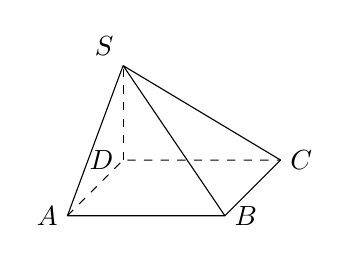
\begin{tikzpicture}
\draw (0,0) node [left] {$A$} coordinate (A)--(2,0) node [right] {$B$} coordinate (B)--({2+0.5*sqrt(2)},{0.5*sqrt(2)}) node [right] {$C$} coordinate (C);
\draw [dashed] (A)--({0.5*sqrt(2)},{0.5*sqrt(2)}) node[left]{$D$} coordinate (D)--(C);
\draw [dashed] (D)--+(0,1.2) node[above left] {$S$} coordinate (S);
\draw (S)--(A) (S)--(B) (S)--(C);
\end{tikzpicture}
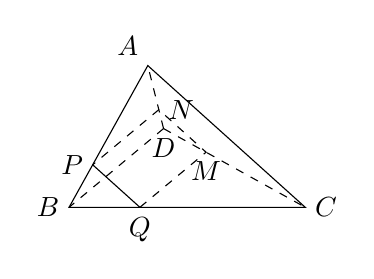
\begin{tikzpicture}
\draw (0,0) coordinate (B) node[left]{$B$}--(3,0) coordinate (C) node [right] {$C$}--(1,1.8) node [above left] {$A$} coordinate (A)--cycle;
\draw [dashed] (1.2,1) node [below]{$D$} coordinate (D)--(A) (D)--(B) (D)--(C);
\coordinate (P) at ($(A)!0.7!(B)$);
\coordinate (Q) at ($(C)!0.7!(B)$);
\coordinate (M) at ($(C)!0.7!(D)$);
\coordinate (N) at ($(A)!0.7!(D)$);
\draw (P) node [left] {$P$}--(Q) node [below] {$Q$};
\draw [dashed] (Q)--(M) node [below] {$M$} --(N) node [right] {$N$} --(P);
\end{tikzpicture}
\end{center}
\newpage


关联目标:

暂未关联目标

答案: 暂无答案

解答或提示: 暂无解答与提示

使用记录:

暂无使用记录


出处: 2016年双基百分百
\item { (003835)}若集合$A=\{x||x-2|\le 2\}$, $B=\{y|y=-x^2, \ -1\le x\le 2\}$, 则$A\cap B=$\blank{50}.


关联目标:

暂未关联目标

答案: 暂无答案

解答或提示: 暂无解答与提示

使用记录:

暂无使用记录


出处: 2016年双基百分百
\item { (003846)}已知$m,n$是两条不同直线, $\alpha,\beta,\gamma$是三个不同平面, 下列命题中正确的是\blank{30}.
\twoch{$m\parallel \alpha$, $n\parallel \alpha$, 则$m\parallel n$}{若$m\parallel \alpha$, $m\parallel \beta$, 则$\alpha\parallel \beta$}{若$\alpha\perp \gamma$, $\beta\perp \gamma$, 则$\alpha\parallel \beta$}{若$m\perp \alpha$, $n\perp \alpha$, 则$m\parallel n$}


关联目标:

暂未关联目标

答案: 暂无答案

解答或提示: 暂无解答与提示

使用记录:

暂无使用记录


出处: 2016年双基百分百
\item { (003860)}若集合$M=\{y|y=x^2-1, \ x\in \mathbf{R}\}$, 集合$N=\{x|y=\sqrt{3-x}, \ x\in \mathbf{R}\}$, 则$M\cap N=$\blank{30}.
\fourch{$\{(-\sqrt{2},1),(\sqrt{2},1)\}$}{$\{t|0\le t\le \sqrt{3}\}$}{$\{t|-1\le t\le 3\}$}{$\{t|-\infty<t\le \sqrt{3}\}$}


关联目标:

暂未关联目标

答案: 暂无答案

解答或提示: 暂无解答与提示

使用记录:

暂无使用记录


出处: 2016年双基百分百
\item { (003865)}集合$\{y|y=2^{-x}\}\cap\{y|y=\lg x, \ 0<x<100\}=$\blank{50}.


关联目标:

暂未关联目标

答案: 暂无答案

解答或提示: 暂无解答与提示

使用记录:

暂无使用记录


出处: 2016年双基百分百
\item { (003884)}已知函数$y=f(x)$的定义域为$\{x|-3\le x\le 8, \ x\ne 5\}$, 值域为$\{y|-1\le y\le 2, \ y\ne 0\}$. 下列关于函数$y=f(x)$的说法: \textcircled{1} 当$x=-3$时, $y=-1$; \textcircled{2} 将$y=f(x)$的图像补上$(5,0)$, 得到的图像必定是一条连续的曲线; \textcircled{3} $y=f(x)$是$[-3,5)$上的单调函数; \textcircled{4} $y=f(x)$的图像与坐标轴只有一个交点. 其中正确的命题是\blank{50}.


关联目标:

暂未关联目标

答案: 暂无答案

解答或提示: 暂无解答与提示

使用记录:

暂无使用记录


出处: 2016年双基百分百
\item { (003887)}从集合$\{1,2,3,4,5,6,7,8,9\}$中任取两个不同的数, 则其中一个数恰是另一个数的$3$倍的概率为\blank{50}.


关联目标:

暂未关联目标

答案: 暂无答案

解答或提示: 暂无解答与提示

使用记录:

暂无使用记录


出处: 2016年双基百分百
\item { (003922)}给出下列类比推理命题($\mathbf{R}$为实数集, $\mathbf{C}$为复数集, $M$为平面向量集), 其中类比结论正确的是\blank{30}.
\onech{由``若$a\in \mathbf{R}$, 则$a^2=|a|^2$''类比推出``若$a\in \mathbf{C}$, 则$a^2=|a|^2$''}{由``若$a,b\in \mathbf{R}$, 且$a-b=0$, 则$a=b$''类比推出``若$\overrightarrow{a},\overrightarrow{b}\in \mathbf{M}$, 且$\overrightarrow a-\overrightarrow b=\overrightarrow 0$, 则$\overrightarrow a=\overrightarrow b$''}{由``若$a,b\in \mathbf{R}$, 且$a^2+b^2=0$, 则$a=0$或$b=0$''类比推出``若$a,b\in \mathbf{C}$, 且$a^2+b^2=0$, 则$a=0$或$b=0$''}{由``若$a,b\in \mathbf{R}$, 且$a\cdot b=0$, 则$a=0$或$b=0$''类比推出``若$\overrightarrow a, \overrightarrow b\in \mathbf{M}$, 且$\overrightarrow a\cdot \overrightarrow b=0$, 则$\overrightarrow a=\overrightarrow 0$或$\overrightarrow b=\overrightarrow 0$''}


关联目标:

暂未关联目标

答案: 暂无答案

解答或提示: 暂无解答与提示

使用记录:

暂无使用记录


出处: 2016年双基百分百
\item { (003925)}已知集合$A=\{x|x^2-2x\le 0 \}$, $B=\{x|-1<x<1\}$, 则$A\cap B=$\blank{50}.


关联目标:

暂未关联目标

答案: 暂无答案

解答或提示: 暂无解答与提示

使用记录:

暂无使用记录


出处: 2016年双基百分百
\item { (003940)}已知集合$A=\{x|x=a+(a^2-1)\mathrm{i}\}$($a\in \mathbf{R}$, $\mathrm{i}$是虚数单位), 若$A\subseteq \mathbf{R}$, 则$a=$\blank{50}.


关联目标:

暂未关联目标

答案: 暂无答案

解答或提示: 暂无解答与提示

使用记录:

暂无使用记录


出处: 2016年双基百分百
\item { (003950)}若$m,n$为两条不同的直线, $\alpha,\beta$为两个不同的平面, 则以下命题正确的是\blank{30}.
\twoch{若$m\parallel \alpha$, $n\parallel\alpha$, 则$m\parallel n$}{若$m\parallel \beta$, $\alpha\parallel\beta$, 则$m\parallel\alpha$}{若$m\parallel n$, $m\perp \alpha$, 则$n\perp \alpha$}{若$\alpha\cap\beta=m$, $m\perp n$, 则$n\perp\alpha$}


关联目标:

暂未关联目标

答案: 暂无答案

解答或提示: 暂无解答与提示

使用记录:

暂无使用记录


出处: 2016年双基百分百
\item { (003953)}已知集合$M$是满足下列性质的函数$f(x)$的全体, 存在非零常数$T$, 对任意$x\in \mathbf{R}$, 有$f(x+T)=Tf(x)$成立.\\
(1) 函数$f(x)=x$是否属于集合$M$? 说明理由;\\
(2) 设$f(x)\in M$, 且$T=2$, 已知当$1<x<2$时, $f(x)=x+\ln x$, 求当$-3<x<-2$时, $f(x)$的解析式.


关联目标:

暂未关联目标

答案: 暂无答案

解答或提示: 暂无解答与提示

使用记录:

暂无使用记录


出处: 2016年双基百分百
\item { (003957)}已知集合$P=\{a,-1\}$, $Q=\{x|x^2-1<0, \ x\in \mathbf{Z}\}$, 如果$P\cap Q\ne\varnothing$, 则实数$a=$\blank{50}.


关联目标:

暂未关联目标

答案: 暂无答案

解答或提示: 暂无解答与提示

使用记录:

暂无使用记录


出处: 2016年双基百分百
\item { (004029)}设集合$A$是由所有满足下面条件的有序数组$(x_1,x_2,x_3,x_4,x_5)$构成的: 每一个元素$x_i$等于$0$、$1$、$-1$中之一, 其中$i=1,2,3,4,5$. 那么集合$A$中满足条件``$1\le |x_1|+|x_2|+|x_3|+|x_4|+|x_5|\le 3$''的元素有多少个?


关联目标:

K0811005X|D08003X|能利用加法原理与乘法原理解决较为复杂的计数问题.

答案: 暂无答案

解答或提示: 暂无解答与提示

使用记录:

暂无使用记录


出处: 教材复习题
\item { (004059)}已知集合$A=\{-2,1,2\}$, $B=\{\sqrt a+1,a\}$, 且$B\subseteq A$, 则实数$a$的值是\blank{50}.


关联目标:

暂未关联目标

答案: $1$

解答或提示: 暂无解答与提示

使用记录:

20220301	2022届高三1班	\fcolorbox[rgb]{0,0,0}{1.000,0.000,0}{1.000}


出处: 2022届高三下学期测验卷01第1题
\item { (004080)}集合$A=\{1,2,3,4\}$, $B=\{x|(x-1)(x-5)<0\}$, 则$A\cap B=$\blank{50}.


关联目标:

暂未关联目标

答案: 暂无答案

解答或提示: 暂无解答与提示

使用记录:

20220308	2022届高三1班	\fcolorbox[rgb]{0,0,0}{1.000,0.046,0}{0.977}


出处: 2022届高三下学期测验卷02第1题
\item { (004091)}已知函数$f(x)=\cos x$, 若对任意实数$x_1$、$x_2$, 方程$|f(x)-f(x_1)|+|f(x)-f(x_2)|=m$($m\in \mathbf{R}$)有解, 方程$|f(x)-f(x_1)|-|f(x)-f(x_2)|=n$($n\in \mathbf{R}$)也有解, 则$m+n$的值的集合为\blank{50}.


关联目标:

暂未关联目标

答案: 暂无答案

解答或提示: 暂无解答与提示

使用记录:

20220308	2022届高三1班	\fcolorbox[rgb]{0,0,0}{0.652,1.000,0}{0.326}


出处: 2022届高三下学期测验卷02第12题
\item { (004110)}非空集合$A$中所有元素乘积记为$T$. 已知集合$M=\{1,4,5,7,8,9\}$ , 从集合$M$的所有非空子集中任选一个子集$A$, 则$T(A)$为偶数的概率是\blank{50}(结果用最简分数表示).


关联目标:

暂未关联目标

答案: 暂无答案

解答或提示: 暂无解答与提示

使用记录:

20220322	2022届高三1班	\fcolorbox[rgb]{0,0,0}{1.000,0.466,0}{0.767}


出处: 2022届高三下学期测验卷03第10题
\item { (004116)}已知集合$M=\{(x,y)|y=f(x)\}$, 若对于任意$(x_1,y_1)\in M$, 存在$(x_2,y_2)\in M$, 使得$x_1x_2+y_1y_2=0$成立, 则称集合$M$是``$\Omega$集合''. 给出下列$4$个集合:
\textcircled{1} $M=\{(x,y) |y=\dfrac 1x \}$; \textcircled{2} $M=\{(x,y)|y=\mathrm{e}^x-2\}$; \textcircled{3} $M=\{(x,y)|y=\cos x\}$; \textcircled{4} $M=\{(x,y)|y=\ln x\}$.
其中所有``$\Omega$集合''的序号是\bracket{20}.
\fourch{\textcircled{2}\textcircled{3}}{\textcircled{3}\textcircled{4}}{\textcircled{1}\textcircled{2}\textcircled{4}}{\textcircled{1}\textcircled{3}\textcircled{4}}


关联目标:

暂未关联目标

答案: 暂无答案

解答或提示: 暂无解答与提示

使用记录:

20220322	2022届高三1班	\fcolorbox[rgb]{0,0,0}{1.000,0.140,0}{0.930}


出处: 2022届高三下学期测验卷03第16题
\item { (004123)}设集合$A=\{1,2,3\}$, $B=\{y|y=\sin x, \ x\in \mathbf{R}\}$, 则$A\cap B=$\blank{50}.


关联目标:

暂未关联目标

答案: 暂无答案

解答或提示: 暂无解答与提示

使用记录:

20220331	2022届高三1班	\fcolorbox[rgb]{0,0,0}{1.000,0.000,0}{1.000}


出处: 2022届高三下学期测验卷04第2题
\item { (004133)}空间中, 给定两条异面直线$m,n$以及平面$\alpha$, 满足: $m\perp n$, $n$在平面$\alpha$上, $m$与$\alpha$所成的角$\theta\in [60^\circ,90^\circ]$. 动点$P$在$\alpha$上, 满足$P$到$m$的距离与$P$到$n$的距离相等, 记$P$的轨迹为曲线$\Gamma$. 对于下列命题: \textcircled{1} $\Gamma$可以是椭圆; \textcircled{2} $\Gamma$可以是双曲线, 且两条渐近线的夹角为$30^\circ$; \textcircled{3} $\Gamma$可以是双曲线, 且两条渐近线的夹角为$60^\circ$; \textcircled{4} $\Gamma$可以是抛物线, 所有真命题的序号为\blank{50}.


关联目标:

暂未关联目标

答案: 暂无答案

解答或提示: 暂无解答与提示

使用记录:

20220331	2022届高三1班	\fcolorbox[rgb]{0,0,0}{0.280,1.000,0}{0.140}


出处: 2022届高三下学期测验卷04第12题
\item { (004137)}在锐角$\triangle ABC$中, $O$为$\triangle ABC$的外心, 设$O$到直线$BC$, $AC$, $AB$的距离分别为$d_1,d_2,d_2$. 若将所有的全等三角形看作同一个三角形, 则对于命题: \textcircled{1} 对任意给定的$d_1,d_2\in \mathbf{R}^+$以及$\angle C\in (0,\dfrac\pi 2)$, 锐角$\triangle ABC$都存在且唯一; \textcircled{2} 对任意给定的$d_1,d_2,d_3\in \mathbf{R}^+$, 锐角$\triangle ABC$都存在且唯一, 下列判断正确的是\bracket{20}.
\twoch{\textcircled{1}、\textcircled{2}均为真命题}{\textcircled{1}、\textcircled{2}均为假命题}{\textcircled{1}为真命题, \textcircled{2}为假命题}{\textcircled{1}为假命题, \textcircled{2}为真命题}


关联目标:

暂未关联目标

答案: 暂无答案

解答或提示: 暂无解答与提示

使用记录:

20220331	2022届高三1班	\fcolorbox[rgb]{0,0,0}{1.000,0.884,0}{0.558}


出处: 2022届高三下学期测验卷04第16题
\item { (004142)}记无穷数列$\{a_n\}$的前$n$项和为$S_n$, 集合$M=\{x|x=a_n, \ n\in \mathbf{N}^*\}$. 若对任意$n\in \mathbf{N}^*$, 恒有$S_n\in M$, 则称$\{a_n\}$具有性质$\mathbf{P}$.\\
(1) 若无穷数列$\{a_n\}$的前$n$项和为$S_n=n^2+n+2$, 判断$\{a_n\}$是否具有性质$\mathbf{P}$, 并说明理由;\\
(2) 若无穷数列$\{a_n\}$为等差数列, 首项$a_1=-1$, 公差$d>0$, 且$\{a_n\}$具有性质$\mathbf{P}$, 求$d$的值;\\
(3) 若无穷数列$\{a_n\}$为等比数列, 首项$a_1=1$, 公比$q>0$, 问: 是否存在$q$, 使得$\{a_n\}$具有性质$\mathbf{P}$? 若存在, 求出所有$q$的值; 若不存在, 说明理由.


关联目标:

暂未关联目标

答案: 暂无答案

解答或提示: 暂无解答与提示

使用记录:

20220331	2022届高三1班	\fcolorbox[rgb]{0,0,0}{1.000,0.046,0}{0.977}	\fcolorbox[rgb]{0,0,0}{1.000,0.364,0}{0.818}	\fcolorbox[rgb]{0,0,0}{0.168,1.000,0}{0.084}


出处: 2022届高三下学期测验卷04第21题
\item { (004144)}已知集合$M=\{x||x+1|\le 1\}$, $N=\{-1,0,1\}$, 则$M\cap N=$\blank{50}.


关联目标:

暂未关联目标

答案: 暂无答案

解答或提示: 暂无解答与提示

使用记录:

20220407	2022届高三1班	\fcolorbox[rgb]{0,0,0}{1.000,0.094,0}{0.953}


出处: 2022届高三下学期测验卷05第2题
\item { (004163)}已知数列$\{x_n\}$, 若对任意$n\in \mathbf{N}^*$, 都有$\dfrac{x_n+x_{n+2}}2>x_{n+1}$, 则称数列$\{x_n\}$为``差增数列''.\\
(1) 试判断数列$a_n=n^2$($n\in \mathbf{N}^*$)是否为``差增数列'', 并说明理由;\\
(2) 对于所有各项均为正整数的``差增数列''$\{a_n\}$, 其中$a_1=a_2=1$, 若使得$a_k=m$成立的序数$k$的最大值为$20$, 求正整数$m$的所有可能取值的集合;\\
(3)若数列$\{\lg x_n\}$为``差增数列''($n\in \mathbf{N}^*$, $n\le 2020$)且$\lg x_1+\lg x_2+\cdots +\lg x_{2020}=0$, 证明: $x_{1010}\cdot x_{1011}<1$.


关联目标:

暂未关联目标

答案: 暂无答案

解答或提示: 暂无解答与提示

使用记录:

20220407	2022届高三1班	\fcolorbox[rgb]{0,0,0}{1.000,0.000,0}{1.000}	\fcolorbox[rgb]{0,0,0}{1.000,0.488,0}{0.756}	\fcolorbox[rgb]{0,0,0}{0.802,1.000,0}{0.401}


出处: 2022届高三下学期测验卷05第21题
\item { (004164)}集合$A=\{x|x^2-2x<0\}$, $B=\{x||x|<1\}$, 则$A\cup B$=\blank{50}.


关联目标:

暂未关联目标

答案: 暂无答案

解答或提示: 暂无解答与提示

使用记录:

20220421	2022届高三1班	\fcolorbox[rgb]{0,0,0}{1.000,0.140,0}{0.930}


出处: 2022届高三下学期测验卷06第1题
\item { (004176)}设$z_1$、$z_2$为复数, 下列命题一定成立的是\bracket{20}.
\onech{如果$z_1^2+z_2^2=0$, 那么$z_1=z_2=0$}{如果$|z_1 |=|z_2 |$, 那么$z_1=\pm z_2$}{如果$|z_1 |\le a$, $a$是正实数, 那么$-a\le {z_1}\le a$}{如果$|z_1|=a$, $a$是正实数, 那么$z_1\cdot \overline{z_1}=a^2$}


关联目标:

暂未关联目标

答案: 暂无答案

解答或提示: 暂无解答与提示

使用记录:

20220421	2022届高三1班	\fcolorbox[rgb]{0,0,0}{1.000,0.000,0}{1.000}


出处: 2022届高三下学期测验卷06第13题
\item { (004177)}下列命题为真命题的是\bracket{20}.
\onech{若直线$l$与平面$\alpha$上的两条直线垂直, 则直线$l$与平面$\alpha$垂直}{若两条直线同时垂直于一个平面, 则这两条直线平行}{若两个平面同时垂直于第三个平面, 则这两个平面垂直}{若直线l上的不同两点到平面$\alpha$的距离相等, 则直线$l$与平面$\alpha$平行}


关联目标:

暂未关联目标

答案: 暂无答案

解答或提示: 暂无解答与提示

使用记录:

20220421	2022届高三1班	\fcolorbox[rgb]{0,0,0}{1.000,0.000,0}{1.000}


出处: 2022届高三下学期测验卷06第14题
\item { (004200)}已知命题: ``若$a,b$为异面直线, 平面$\alpha$过直线$a$且与直线$b$平行, 则直线$b$与平面$\alpha$的距离等于异面直线$a,b$之间的距离''为真命题.
根据上述命题, 若$a,b$为异面直线, 且它们之间的距离为$d$, 则空间中与$a,b$均异面
且距离也均为$d$的直线$c$的条数为\bracket{20}.
\twoch{$0$条}{$1$条}{多于$1$条, 但为有限条}{无数多条}


关联目标:

暂未关联目标

答案: 暂无答案

解答或提示: 暂无解答与提示

使用记录:

20220428	2022届高三1班	\fcolorbox[rgb]{0,0,0}{1.000,0.372,0}{0.814}


出处: 2022届高三下学期测验卷07第16题
\item { (004218)}给出下列命题, 其中正确的命题为\bracket{20}.
\onech{若直线$a$和$b$共面, 直线$b$和$c$共面, 则$a$和$c$共面}{直线$a$与平面$\alpha$不垂直, 则$a$与平面$\alpha$内的所有直线都不垂直}{直线$a$与平面$\alpha$不平行, 则$a$与平面$\alpha$内的所有直线都不平行}{异面直线$a$、$b$不垂直, 则过$a$的任何平面与$b$都不垂直}


关联目标:

暂未关联目标

答案: 暂无答案

解答或提示: 暂无解答与提示

使用记录:

20220505	2022届高三1班	\fcolorbox[rgb]{0,0,0}{1.000,0.232,0}{0.884}


出处: 2022届高三下学期测验卷08第13题
\item { (004221)}在圆锥$PO$中, 已知高$PO=2$, 底面圆的直径$AB=8$, $M$为母线$PB$的中点. 根据圆锥曲线的定义, 下列四个图中的截面边界曲线分别为圆(截面平行于底面)、椭圆(椭圆长轴为线段$AM$)、双曲线的一部分(双曲线所在平面垂直于$AB$)及抛物线的一部分(抛物线对称轴为$MO$所在直线), 下面四个命题:\\
\textcircled{1} 圆的面积为$4\pi$; \textcircled{2} 椭圆的长轴为$\sqrt{37}$; \textcircled{3} 双曲线两渐近线的夹角为$\arcsin \dfrac 35$; \textcircled{4} 抛物线中焦点到准线的距离为$\dfrac{8\sqrt 5}5$中, 正确的个数为\bracket{20}.
\begin{center}
    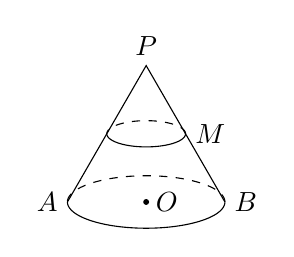
\begin{tikzpicture}
        \draw (1,{-sqrt(3)}) node [right] {$B$} -- (0,0) node [above] {$P$} -- (-1,{-sqrt(3)}) node [left] {$A$};
        \draw [domain = 90:270,samples = 200,dashed] plot ({1/2*sin(\x)},{-1/6*(cos(\x))-sqrt(3)/2});
        \draw [domain = 90:-90,samples = 200] plot ({1/2*sin(\x)},{-1/6*(cos(\x))-sqrt(3)/2});
        \draw [domain = 90:270,samples = 200,dashed] plot ({sin(\x)},{-1/3*(cos(\x))-sqrt(3)});
        \draw [domain = 90:-90,samples = 200] plot ({sin(\x)},{-1/3*(cos(\x))-sqrt(3)});
        \filldraw (0,{-sqrt(3)}) circle (0.03) node [right] {$O$} ({1/2},{-sqrt(3)/2}) node [right] {$M$};
    \end{tikzpicture}
    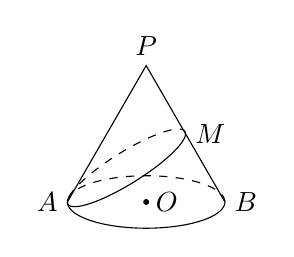
\begin{tikzpicture}
        \draw (1,{-sqrt(3)}) node [right] {$B$} -- (0,0) node [above] {$P$} -- (-1,{-sqrt(3)}) node [left] {$A$};
        \draw [domain = 90:270,samples = 200,dashed] plot ({2*sin(\x)/(3+sin(\x))},{-1/3*2*cos(\x)/(3+sin(\x))-2*sqrt(3)/(3+sin(\x))});
        \draw [domain = 90:-90,samples = 200] plot ({2*sin(\x)/(3+sin(\x))},{-1/3*2*cos(\x)/(3+sin(\x))-2*sqrt(3)/(3+sin(\x))});
        \draw [domain = 90:270,samples = 200,dashed] plot ({sin(\x)},{-1/3*(cos(\x))-sqrt(3)});
        \draw [domain = 90:-90,samples = 200] plot ({sin(\x)},{-1/3*(cos(\x))-sqrt(3)});
        \filldraw (0,{-sqrt(3)}) circle (0.03) node [right] {$O$} ({1/2},{-sqrt(3)/2}) node [right] {$M$};
    \end{tikzpicture}
    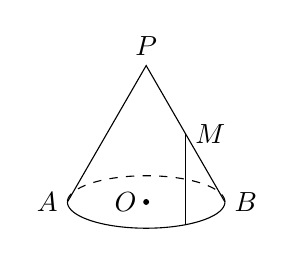
\begin{tikzpicture}
        \draw (1,{-sqrt(3)}) node [right] {$B$} -- (0,0) node [above] {$P$} -- (-1,{-sqrt(3)}) node [left] {$A$};
        \draw [domain = 30:90,samples = 200,dashed] plot ({1/2},{cos(\x)/6/sin(\x)-sqrt(3)/2/sin(\x)});
        \draw [domain = 150:90,samples = 200] plot ({1/2},{cos(\x)/6/sin(\x)-sqrt(3)/2/sin(\x)});
        \draw [domain = 90:270,samples = 200,dashed] plot ({sin(\x)},{-1/3*(cos(\x))-sqrt(3)});
        \draw [domain = 90:-90,samples = 200] plot ({sin(\x)},{-1/3*(cos(\x))-sqrt(3)});
        \filldraw (0,{-sqrt(3)}) circle (0.03) node [left] {$O$} ({1/2},{-sqrt(3)/2}) node [right] {$M$};
    \end{tikzpicture}
    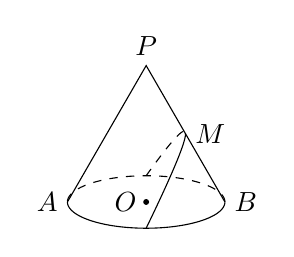
\begin{tikzpicture}
        \draw (1,{-sqrt(3)}) node [right] {$B$} -- (0,0) node [above] {$P$} -- (-1,{-sqrt(3)}) node [left] {$A$};
        \draw [domain = 0:90,samples = 200,dashed] plot ({sin(\x)/(1+sin(\x))},{1/3*cos(\x)/(1+sin(\x))-sqrt(3)/(1+sin(\x))});
        \draw [domain = 180:90,samples = 200] plot ({sin(\x)/(1+sin(\x))},{1/3*cos(\x)/(1+sin(\x))-sqrt(3)/(1+sin(\x))});
        \draw [domain = 90:270,samples = 200,dashed] plot ({sin(\x)},{-1/3*(cos(\x))-sqrt(3)});
        \draw [domain = 90:-90,samples = 200] plot ({sin(\x)},{-1/3*(cos(\x))-sqrt(3)});
        \filldraw (0,{-sqrt(3)}) circle (0.03) node [left] {$O$} ({1/2},{-sqrt(3)/2}) node [right] {$M$};
    \end{tikzpicture}
\end{center}
\fourch{$1$个}{$2$个}{$3$个}{$4$个}


关联目标:

暂未关联目标

答案: 暂无答案

解答或提示: 暂无解答与提示

使用记录:

20220505	2022届高三1班	\fcolorbox[rgb]{0,0,0}{1.000,0.372,0}{0.814}


出处: 2022届高三下学期测验卷08第16题
\item { (004226)}给定无穷数列$\{a_n\}$, 若无穷数列$\{b_n\}$满足: 对任意$n\in \mathbf{N}^*$, 都有$|b_n-a_n|\le 1$, 则称$\{a_n\}$与$\{b_n\}$ ``接近''.\\
(1) 设$\{a_n\}$是首项为$1$, 公比为$\dfrac 12$的等比数列, $b_n=a_{n+1}+1$, $n\in \mathbf{N}^*$, 判断数列$\{b_n\}$是否与$\{a_n\}$接近, 并说明理由;\\
(2) 设数列$\{a_n\}$的前四项为: $a_1=1$, $a_2=2$, $a_3=4$, $a_4=8$ , $\{b_n\}$是一个与$\{a_n\}$接近的数列, 记集合$M=\{x|x=b_i,\ i=1,2,3,4\}$, 求$M$中元素的个数$m$的所有可能值;\\
(3) 已知$\{a_n\}$是公差为$d$的等差数列, 若存在数列$\{b_n\}$满足: $\{b_n\}$与$\{a_n\}$接近, 且在$b_2-b_1,b_3-b_2,\cdots,b_{201}-b_{200}$中至少有$100$个为正数, 求$d$的取值范围.


关联目标:

暂未关联目标

答案: 暂无答案

解答或提示: 暂无解答与提示

使用记录:

20220505	2022届高三1班	\fcolorbox[rgb]{0,0,0}{1.000,0.186,0}{0.907}	\fcolorbox[rgb]{0,0,0}{1.000,0.798,0}{0.601}	\fcolorbox[rgb]{0,0,0}{1.000,0.976,0}{0.512}


出处: 2022届高三下学期测验卷08第21题
\item { (004227)}已知集合$A=\{1,3,m\}$, $B=\{3,5\}$, 且$B\subseteq A$, 则实数$m$的值是\blank{50}.


关联目标:

暂未关联目标

答案: 暂无答案

解答或提示: 暂无解答与提示

使用记录:

20220512	2022届高三1班	\fcolorbox[rgb]{0,0,0}{1.000,0.000,0}{1.000}


出处: 2022届高三下学期测验卷09第1题
\item { (004271)}若集合$A=\{2,4,6,8\}$, $B=\{x|x^2-4x\le 0\}$, 则$A\cap B=$\blank{50}.


关联目标:

暂未关联目标

答案: 暂无答案

解答或提示: 暂无解答与提示

使用记录:

20220524	2022届高三1班	\fcolorbox[rgb]{0,0,0}{1.000,0.000,0}{1.000}


出处: 2022届高三下学期测验卷11第3题
\item { (004284)}已知函数$f(x)=m\cdot 2^x+x^2+nx$, 记集合$A=\{x|f(x)=0, \ x\in \mathbf{R}\}$, 集合$B=\{x|f(f(x))=0, \ x\in \mathbf{R}\}$.
若$A=B$, 且$A$、$B$都不是空集, 则$m+n$的取值范围是\bracket{20}.
\fourch{$[0,4)$}{$[-1,4)$}{$[-3,5]$}{$[0,7)$}


关联目标:

暂未关联目标

答案: 暂无答案

解答或提示: 暂无解答与提示

使用记录:

20220524	2022届高三1班	\fcolorbox[rgb]{0,0,0}{1.000,0.186,0}{0.907}


出处: 2022届高三下学期测验卷11第16题
\item { (004292)}已知集合$P=\{x|(x+1)(x–3)<0\}$, $Q=\{x||x|>2\}$, 则$P\cap Q=$\blank{50}.


关联目标:

暂未关联目标

答案: 暂无答案

解答或提示: 暂无解答与提示

使用记录:

20220607	2022届高三1班	\fcolorbox[rgb]{0,0,0}{1.000,0.094,0}{0.953}


出处: 2022届高三下学期测验卷12第3题
\item { (004299)}平面上三条直线$x-2y+1=0$, $x-1=0$, $x+ky=0$, 如果这三条直线将平面划分为六个部分, 则实数$k$的取值组成的集合$A=$\blank{50}.


关联目标:

暂未关联目标

答案: 暂无答案

解答或提示: 暂无解答与提示

使用记录:

20220607	2022届高三1班	\fcolorbox[rgb]{0,0,0}{1.000,0.418,0}{0.791}


出处: 2022届高三下学期测验卷12第10题
\item { (004305)}定义$F(a,b)=\begin{cases} a, & a \le b, \\ b, & a>b,\end{cases}$, 已知函数$f(x)$、$g(x)$定义域都是$\mathbf{R}$, 给出下列命题:\\
(1) 若$f(x)$、$g(x)$都是奇函数, 则函数$F(f(x),g(x))$为奇函数;\\
(2) 若$f(x)$、$g(x)$都是减函数, 则函数$F(f(x),g(x))$为减函数;\\
(3) 若$f_{\min}(x)=m$, $g_{\min}(x)=n$, 则$F_{\min}(f(x),g(x))=F(m,n)$;\\
(4) 若$f(x)$、$g(x)$都是周期函数, 则函数$F(f(x),g(x))$是周期函数.\\
其中正确命题的个数为\bracket{20}.
\fourch{$1$个}{$2$个}{$3$个}{$4$个}


关联目标:

暂未关联目标

答案: 暂无答案

解答或提示: 暂无解答与提示

使用记录:

20220607	2022届高三1班	\fcolorbox[rgb]{0,0,0}{0.512,1.000,0}{0.256}


出处: 2022届高三下学期测验卷12第16题
\item { (004311)}设$m\in \mathbf{R}$. 已知集合$A=\{2,3\}$, $B=\{1,m\}$. 若$4-m\in A$, 则$m=$\blank{50}.


关联目标:

暂未关联目标

答案: 暂无答案

解答或提示: 暂无解答与提示

使用记录:

20220627	2022届高三1班	\fcolorbox[rgb]{0,0,0}{1.000,0.000,0}{1.000}


出处: 2022届高三下学期测验卷13第1题
\item { (004330)}双曲线$\Gamma$: $x^2-\dfrac{y^2}{b^2}=1$($b>0$).\\
(1) 若$\Gamma$的一条渐近线方程为$y=2x$, 求$\Gamma$的方程;\\
(2) 设$F_1$、$F_2$是$\Gamma$的两个焦点, $P$为$\Gamma$上一点, 且$PF_1\perp PF_2$, $\triangle PF_1F_2$的面积为$9$, 求$b$的值;\\
(3) 已知斜率为$2$的直线与$\Gamma$交于$A$、$B$两点, 点$M$是线段$AB$的中点, 设点$M$的横坐标的集合为$\Omega$. 若$\{x|x=2n,\ n\in \mathbf{N}^* \}\subseteq \Omega$, 求正数$b$的取值范围.


关联目标:

暂未关联目标

答案: 暂无答案

解答或提示: 暂无解答与提示

使用记录:

20220627	2022届高三1班	\fcolorbox[rgb]{0,0,0}{1.000,0.000,0}{1.000}	\fcolorbox[rgb]{0,0,0}{1.000,0.132,0}{0.934}	\fcolorbox[rgb]{0,0,0}{1.000,0.720,0}{0.640}


出处: 2022届高三下学期测验卷13第20题
\item { (004343)}设$P_1P_2P_3\cdots P_8$是平面直角坐标系中的一个正八边形, 点$P_i$的坐标为$(x_i,y_i) \ (i=1,2,\cdots,8)$. 集合$A=\{y|\text{存在} i\in \{1,2,\cdots,8\},\text{ 使得 }y=y_i\}$, 则集合$A$的元素个数可能为\blank{50}(写出所有可能的值).


关联目标:

暂未关联目标

答案: 暂无答案

解答或提示: 暂无解答与提示

使用记录:

20220630	2022届高三1班	\fcolorbox[rgb]{0,0,0}{1.000,0.232,0}{0.884}


出处: 2022届高三下学期测验卷14第12题
\item { (004347)}已知$y=f(x)$与$y=g(x)$皆是定义域、值域均为$\mathbf{R}$的函数. 若对任意$x\in \mathbf{R}$, $f(x)>g(x)$恒成立, 且$y=f(x)$与$y=g(x)$的反函数$y=f^{-1}(x)$、$y=g^{-1}(x)$均存在. 命题$P$: ``对任意$x\in \mathbf{R}$, $f^{-1}(x)<g^{-1}(x)$恒成立''; 命题$Q$: ``函数$y=f(x)+g(x)$的反函数一定存在''. 以下关于这两个命题的真假判断, 正确的是\bracket{20}.
\twoch{命题$P$真, 命题$Q$真}{命题$P$真, 命题$Q$假
}{命题$P$假, 命题$Q$真}{命题$P$假, 命题$Q$假}


关联目标:

暂未关联目标

答案: 暂无答案

解答或提示: 暂无解答与提示

使用记录:

20220630	2022届高三1班	\fcolorbox[rgb]{0,0,0}{0.884,1.000,0}{0.442}


出处: 2022届高三下学期测验卷14第16题
\item { (004353)}已知全集$U=\{x|x<2\}$, 集合$A=\{x|x<1\}$, 则$\complement_UA=$\blank{50}.


关联目标:

暂未关联目标

答案: 暂无答案

解答或提示: 暂无解答与提示

使用记录:

20210918	2022届高三1班	\fcolorbox[rgb]{0,0,0}{1.000,0.046,0}{0.977}


出处: 2022届高三上学期测验卷01第1题
\item { (004354)}设集合$A=\{x||x-2|<1, \ x\in\mathbf{R}\}$, $B=\{x|\dfrac{x-3}{x-1}\ge 0\}$, 则$A\cup B=$\blank{50}.


关联目标:

暂未关联目标

答案: 暂无答案

解答或提示: 暂无解答与提示

使用记录:

20210918	2022届高三1班	\fcolorbox[rgb]{0,0,0}{1.000,0.140,0}{0.930}


出处: 2022届高三上学期测验卷01第2题
\item { (004374)}设集合$A=\{1,2,3\}$, $B=\{x|x<3\}$, 则$A\cap B=$\blank{50}.


关联目标:

暂未关联目标

答案: 暂无答案

解答或提示: 暂无解答与提示

使用记录:

20210928	2022届高三1班	\fcolorbox[rgb]{0,0,0}{1.000,0.000,0}{1.000}


出处: 2022届高三上学期测验卷02第1题
\item { (004382)}已知常数$m,n\in \mathbf{Z}$, 若对任意$x\in [0,+\infty)$, 不等式$(mx-2)(x^2-2n)\ge 0$恒成立, 则$m+n$的取值集合为\blank{50}.


关联目标:

暂未关联目标

答案: 暂无答案

解答或提示: 暂无解答与提示

使用记录:

20210928	2022届高三1班	\fcolorbox[rgb]{0,0,0}{1.000,0.326,0}{0.837}


出处: 2022届高三上学期测验卷02第9题
\item { (004385)}设函数$f(x)$的定义域为$\mathbf{R}$, $f(x)$满足对任意$x_1,x_2\in \mathbf{R}$, 当$x_1\ne x_2$时, 恒有$|f(x_1)-f(x_2)|>2|x_1-x_2|$. 对于命题: \textcircled{1} $f(x)$的解析式可以是$f(x)=x^3+2021x$; \textcircled{2} $f(x)$的解析式可以是$f(x)=2021^{-x}$, 下列判断正确的是\bracket{20}.
\twoch{\textcircled{1}、\textcircled{2}均为真命题}{\textcircled{1}、\textcircled{2}均为假命题}{\textcircled{1}为真命题、\textcircled{2}为假命题}{\textcircled{1}为假命题、\textcircled{2}为真命题}


关联目标:

暂未关联目标

答案: 暂无答案

解答或提示: 暂无解答与提示

使用记录:

20210928	2022届高三1班	\fcolorbox[rgb]{0,0,0}{1.000,0.000,0}{1.000}


出处: 2022届高三上学期测验卷02第12题
\item { (004399)}对于全集$\mathbf{R}$的子集$A$, 定义函数$f_A(x)=\begin{cases}
1, &  x\in A,  \\0, & x\in \complement_{\mathbf{R}}A  \end{cases}$为$A$的特征函数, 设$A,B$为全集$\mathbf{R}$的子集,\\
\textcircled{1} 若$A\subseteq B$, 则$f_A(x)\le f_B(x)$; \textcircled{2} $f_{\complement_{\mathbf{R}}A}(x)=1-f_A(x)$;\\
\textcircled{3} ${f_{A\cap B}}(x)=f_A(x)\cdot f_B(x)$; \textcircled{4} $f_{A\cup B}(x)=f_A(x)+f_B(x)$;\\ \textcircled{5} $f_{A\cap \complement_\mathbf{R}B}(x)=f_A(x)-f_B(x)$; \textcircled{6} 对于任意$x\in \mathbf{R}$, 若$f_A(x)\cdot f_B(x)=0$恒成立, 则$A\cap B=\varnothing$.\\
其中正确的命题为\blank{50}(填所有正确命题的序号).


关联目标:

暂未关联目标

答案: 暂无答案

解答或提示: 暂无解答与提示

使用记录:

20211012	2022届高三1班	\fcolorbox[rgb]{0,0,0}{1.000,0.590,0}{0.705}


出处: 2022届高三上学期测验卷03第12题
\item { (004403)}设集合$A=\{y|y=a^x,\ x>0\}$(其中常数$a>0,  \ a\ne 1$), $B=\{y|y=x^k,\ x\in A\}$(其中常数$k\in \mathbf{Q}$), 则``$k<0$''是``$A\cap B=\varnothing$''的\bracket{20}.
\twoch{充分非必要条件}{必要非充分条件}{充分必要条件}{既非充分又非必要条件}


关联目标:

暂未关联目标

答案: 暂无答案

解答或提示: 暂无解答与提示

使用记录:

20211012	2022届高三1班	\fcolorbox[rgb]{0,0,0}{1.000,0.954,0}{0.523}


出处: 2022届高三上学期测验卷03第16题
\item { (004414)}已知集合$M=\{y|y=3\sin x,x\in \mathbf{R}\}$, $N=\{x||x|<a\}$, 若$M\subseteq N$, 则实数$a$的取值范围是\blank{50}.


关联目标:

暂未关联目标

答案: 暂无答案

解答或提示: 暂无解答与提示

使用记录:

20211018	2022届高三1班	\fcolorbox[rgb]{0,0,0}{1.000,0.142,0}{0.929}


出处: 2022届高三上学期测验卷04第6题
\item { (004421)}已知$M$、$N$、$P\subseteq \mathbf{R}$, $M=\{x|f(x)=0\}$, $N=\{x|g(x)=0\}$, $P=\{x|f(x)g(x)=0\}$, 则集合$P$恒满足的关系为\bracket{20}.
\fourch{$P=M\cup N$}{$P\ne \varnothing$}{$P=\varnothing$}{$P\subseteq (M\cup N)$}


关联目标:

暂未关联目标

答案: 暂无答案

解答或提示: 暂无解答与提示

使用记录:

20211018	2022届高三1班	\fcolorbox[rgb]{0,0,0}{1.000,0.238,0}{0.881}


出处: 2022届高三上学期测验卷04第13题
\item { (004422)}已知$a_1$、$a_2$与$b_1$、$b_2$是$4$个不同的实数, 关于x的方程$|x-a_1|+|x-a_2|=|x-b_1|+|x-b_2|$的解集为$A$, 则集合$A$中元素的个数为\bracket{20}.
\twoch{$1$个}{$0$个或$1$个或$2$个}{$0$个或$1$个或$2$个或无限个}{$1$个或无限个}


关联目标:

暂未关联目标

答案: 暂无答案

解答或提示: 暂无解答与提示

使用记录:

20211018	2022届高三1班	\fcolorbox[rgb]{0,0,0}{0.952,1.000,0}{0.476}


出处: 2022届高三上学期测验卷04第14题
\item { (004424)}设$\mu (x)$表示不小于$x$的最小整数, 例如$\mu(0.3)=1$, $\mu(-2.5)=2$.\\
(1) 解方程$\mu(x-1)=3$;\\
(2) 设$f(x)=\mu (x\cdot \mu (x))$, $n\in \mathbf{N}^*$, 试分别求出$f(x)$在区间$(0,1]$、$(1,2]$以及$(2,3]$上的值域; 若$f(x)$在区间$(0,n]$上的值域为$M_n$, 求集合$M_n$中的元素的个数;\\
(3) 设实数$a>0$, $g(x)=x+a\cdot \dfrac{\mu (x)}x-2$, $h(x)=\dfrac{\sin (\pi x)+2}{x^2-5x+7}$, 若对于任意$x_1,x_2\in (2,4]$都有$g(x_1)>h(x_2)$, 求实数$a$的取值范围.


关联目标:

暂未关联目标

答案: 暂无答案

解答或提示: 暂无解答与提示

使用记录:

20211018	2022届高三1班	\fcolorbox[rgb]{0,0,0}{1.000,0.226,0}{0.887}	\fcolorbox[rgb]{0,0,0}{1.000,0.666,0}{0.667}	\fcolorbox[rgb]{0,0,0}{1.000,0.960,0}{0.520}


出处: 2022届高三上学期测验卷04第16题
\item { (004432)}集合$\{x|\cos(\pi \cos x)=0,\ x\in [0,\pi]\}=$\blank{50}(用列举法表示).


关联目标:

暂未关联目标

答案: 暂无答案

解答或提示: 暂无解答与提示

使用记录:

20211026	2022届高三1班	\fcolorbox[rgb]{0,0,0}{1.000,0.094,0}{0.953}


出处: 2022届高三上学期测验卷05第8题
\item { (004435)}集合$A=\{y|y=\log_{\frac 12}x-x,1\le x\le 2\}$, $B=\{x|x^2-5tx+1\le 0\}$, 若$A\cap B=A$, 则实数$t$的取值范围是\blank{50}.


关联目标:

暂未关联目标

答案: 暂无答案

解答或提示: 暂无解答与提示

使用记录:

20211026	2022届高三1班	\fcolorbox[rgb]{0,0,0}{1.000,0.326,0}{0.837}


出处: 2022届高三上学期测验卷05第11题
\item { (004460)}已知二面角$\alpha-l-\beta$是直二面角, $m$为直线, $\gamma$为平面, 则下列命题中真命题为\bracket{20}.
\twoch{若$m\subsetneqq \alpha$, 则$m\perp \beta$}{若$m\perp \alpha$, 则$m\parallel \beta$}{若$m\parallel \alpha$, 则$m\perp \beta$}{若$\gamma\parallel \alpha$, 则$\gamma\perp \beta$}


关联目标:

暂未关联目标

答案: 暂无答案

解答或提示: 暂无解答与提示

使用记录:

20211102	2022届高三1班	\fcolorbox[rgb]{0,0,0}{1.000,0.096,0}{0.952}


出处: 2022届高三上学期测验卷06第15题
\item { (004468)}设全集$U=\mathbf{R}$集合$A=\{-2,-1,0,1,2\}$, $B=\{x|x\ge 0\}$, 则$A\cap \complement_UB=$\blank{50}.


关联目标:

暂未关联目标

答案: 暂无答案

解答或提示: 暂无解答与提示

使用记录:

20211116	2022届高三1班	\fcolorbox[rgb]{0,0,0}{1.000,0.000,0}{1.000}


出处: 2022届高三上学期测验卷07第2题
\item { (004499)}已知集合$M=\{1,2,3,\cdots,10\}$, 集合$A\subseteq M$, 定义$M(A)$为$A$中元素的最大值, 当$A$取遍$M$的所有非空子集时, 对应的$M(A)$的和记为$S_{10}$, 则$S_{10}=$\blank{50}.


关联目标:

暂未关联目标

答案: 暂无答案

解答或提示: 暂无解答与提示

使用记录:

20211123	2022届高三1班	\fcolorbox[rgb]{0,0,0}{0.286,1.000,0}{0.143}


出处: 2022届高三上学期测验卷08第12题
\item { (004510)}已知集合$A=\{x|x>0\}$, $B=\{x|x^2\le 1\}$, 则$A\cap B=$\blank{50}.


关联目标:

暂未关联目标

答案: 暂无答案

解答或提示: 暂无解答与提示

使用记录:

20211129	2022届高三1班	\fcolorbox[rgb]{0,0,0}{1.000,0.046,0}{0.977}


出处: 2022届高三上学期测验卷09第2题
\item { (004520)}设函数$f(x)=|x-a|-\dfrac 2x+a$, 若关于$x$的方程$f(x)=1$有且仅有两个不同的实数根, 则实数$a$的取值构成的集合为\blank{50}.


关联目标:

暂未关联目标

答案: 暂无答案

解答或提示: 暂无解答与提示

使用记录:

20211129	2022届高三1班	\fcolorbox[rgb]{0,0,0}{1.000,0.418,0}{0.791}


出处: 2022届高三上学期测验卷09第12题
\item { (004525)}已知函数$f(x)=\begin{cases} x^2, & x\text{为无理数}, \\ x, &x\text{为有理数},   \end{cases}$ 则以下$4$个命题:
\textcircled{1} $f(x)$是偶函数; \textcircled{2} $f(x)$在$[0,+\infty)$上是增函数; \textcircled{3} $f(x)$的值域为$\mathbf{R}$; \textcircled{4} 对于任意的正有理数$a$, $g(x)=f(x)-a$存在奇数个零点.
其中正确命题的个数为\bracket{20}.
\fourch{$0$}{$1$}{$2$}{$3$}


关联目标:

暂未关联目标

答案: 暂无答案

解答或提示: 暂无解答与提示

使用记录:

20211129	2022届高三1班	\fcolorbox[rgb]{0,0,0}{1.000,0.032,0}{0.984}	\fcolorbox[rgb]{0,0,0}{1.000,0.058,0}{0.971}


出处: 2022届高三上学期测验卷09第17题
\item { (004552)}已知集合$A=\{1,2,3,4,5\}$, $B=\{3,5,6\}$, 则$A\cap B=$\blank{50}.


关联目标:

暂未关联目标

答案: 暂无答案

解答或提示: 暂无解答与提示

使用记录:

20211228	2022届高三1班	\fcolorbox[rgb]{0,0,0}{1.000,0.000,0}{1.000}


出处: 2022届高三上学期测验卷11第2题
\item { (004562)}已知$t\in \mathbf{R}$, 集合$A=[t,t+1]\cup [t+4,t+9]$, 且$0\not\in A$. 若存在正数$\lambda$, 对任意$a\in A$, 都有$\dfrac{\lambda}a\in A$, 则$t$的值为\blank{50}.


关联目标:

暂未关联目标

答案: 暂无答案

解答或提示: 暂无解答与提示

使用记录:

20211228	2022届高三1班	\fcolorbox[rgb]{0,0,0}{0.772,1.000,0}{0.386}


出处: 2022届高三上学期测验卷11第12题
\item { (004571)}若$\{a_n\}$是等差数列, 公差$d\in (0,\pi]$, 数列$\{b_n\}$满足: $b_n=\sin (a_n)$, $n \in \mathbf{N}^*$, 记$S=\{x|x=b_n, \ n\in \mathbf{N}^*\}$.\\
(1) 设$a_1=0$, $d=\dfrac 23 \pi$, 求集合$S$;\\
(2) 设$a_1=\dfrac\pi 2$, 试求$d$的值, 使得集合$S$恰有两个元素;\\
(3) 若集合$S$恰有三个元素, 且$b_{n+T}=b_n$, 其中$T$为不超过$7$的正整数, 求$T$的所有可能值.


关联目标:

暂未关联目标

答案: 暂无答案

解答或提示: 暂无解答与提示

使用记录:

20211228	2022届高三1班	\fcolorbox[rgb]{0,0,0}{1.000,0.056,0}{0.972}	\fcolorbox[rgb]{0,0,0}{1.000,0.576,0}{0.712}	\fcolorbox[rgb]{0,0,0}{0.728,1.000,0}{0.364}


出处: 2022届高三上学期测验卷11第21题
\item { (004630)}已知集合$A=\{x|x=2n-1, \ n\in \mathbf{N}^*\}$, $B=\{x|x=2^k, \ k\in \mathbf{N}^*\}$. 将$A\cup B$的所有元素从小到大依次排列构成一个数列$\{a_n\}$. 记$S_n$为数列$\{a_n\}$的前$n$项和, 则使得$a_n\in A$与${S_{n-1}}>100{a_n}$同时成立的正整数$n$的最小值为\blank{50}.


关联目标:

暂未关联目标

答案: 暂无答案

解答或提示: 暂无解答与提示

使用记录:

20210924	2022届高三1班	\fcolorbox[rgb]{0,0,0}{0.454,1.000,0}{0.227}

20210924	2022届高三	\fcolorbox[rgb]{0,0,0}{0.130,1.000,0}{0.065}


出处: 2022届高三上月考卷01第12题
\item { (004637)}设函数$f(x)=\cos^2x-2\sin x\cos x+3\sin^2x$.\\
(1) 求使$f(x)$取得最大值的$x$的集合;\\
(2) 设$x_1,x_2\in \mathbf{R}^+$, 且$f(x_1)+f(x_2)=4$. 求证: $x_1+x_2\ge \dfrac{\pi}2$.


关联目标:

暂未关联目标

答案: 暂无答案

解答或提示: 暂无解答与提示

使用记录:

20210924	2022届高三1班	\fcolorbox[rgb]{0,0,0}{1.000,0.196,0}{0.902}	\fcolorbox[rgb]{0,0,0}{1.000,0.624,0}{0.688}

20210924	2022届高三	\fcolorbox[rgb]{0,0,0}{1.000,0.530,0}{0.735}	\fcolorbox[rgb]{0,0,0}{0.816,1.000,0}{0.408}


出处: 2022届高三上月考卷01第19题
\item { (004651)}已知数列$\{a_n\}$的前$n$项和为$S_n$, 且$a_n+a_{n+1}=\dfrac 1{2^n}$, 若数列$\{S_n\}$收敛于常数$A$, 则首项$a_1$取值的集合为\blank{50}.


关联目标:

暂未关联目标

答案: 暂无答案

解答或提示: 暂无解答与提示

使用记录:

20211209	2022届高三1班	\fcolorbox[rgb]{0,0,0}{1.000,0.954,0}{0.523}

20211209	2022届高三	\fcolorbox[rgb]{0,0,0}{0.322,1.000,0}{0.161}


出处: 2022届高三上月考卷02第12题
\item { (004655)}已知正方体$ABCD-A_1B_1C_1D_1$, 点$P$是棱$CC_1$的中点, 设直线$AB$为$a$, 直线$A_1D_1$为$b$.对于下列两个命题: \textcircled{1} 过点$P$有且只有一条直线$l$与$a$、$b$都相交; \textcircled{2} 过点$P$有且只有一条直线$l$与$a$、$b$都成$45^\circ$角. 以下判断正确的是\bracket{20}.
\begin{center}
    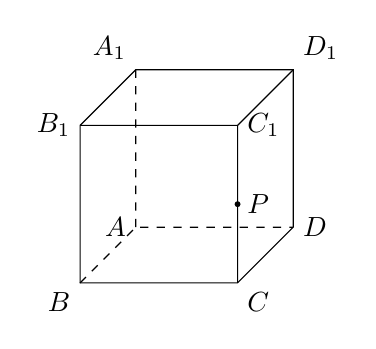
\begin{tikzpicture}
        \draw (0,0) node [below left] {$B$} coordinate (B) --++ (2,0) node [below right] {$C$} coordinate (C) --++ (45:{2/2}) node [right] {$D$} coordinate (D)
        --++ (0,2) node [above right] {$D_1$} coordinate (D1)
        --++ (-2,0) node [above left] {$A_1$} coordinate (A1) --++ (225:{2/2}) node [left] {$B_1$} coordinate (B1) -- cycle;
        \draw (B) ++ (2,2) node [right] {$C_1$} coordinate (C1) -- (C) (C1) --++ (45:{2/2}) (C1) --++ (-2,0);
        \draw [dashed] (B) --++ (45:{2/2}) node [left] {$A$} coordinate (A) --++ (2,0) (A) --++ (0,2);
        \filldraw ($(C)!0.5!(C1)$) node [right] {$P$} circle (0.03);
    \end{tikzpicture}
\end{center}
\twoch{\textcircled{1} 为真命题, \textcircled{2} 为真命题}{\textcircled{1} 为真命题, \textcircled{2} 为假命题}{\textcircled{1} 为假命题, \textcircled{2} 为真命题}{\textcircled{1} 为假命题, \textcircled{2} 为假命题}


关联目标:

暂未关联目标

答案: 暂无答案

解答或提示: 暂无解答与提示

使用记录:

20211209	2022届高三1班	\fcolorbox[rgb]{0,0,0}{1.000,0.500,0}{0.750}

20211209	2022届高三	\fcolorbox[rgb]{0,0,0}{0.956,1.000,0}{0.478}


出处: 2022届高三上月考卷02第16题
\item { (004662)}集合$A=\{-1, 2m-1\}$, $B=\{m^2\}$, 若$B\subseteq A$, 则实数$m=$\blank{50}.


关联目标:

暂未关联目标

答案: 暂无答案

解答或提示: 暂无解答与提示

使用记录:

20211109	2022届高三	\fcolorbox[rgb]{0,0,0}{1.000,0.012,0}{0.994}


出处: 2022届高三上期中区统考第2题
\item { (004676)}非空集合$A\subseteq \mathbf{R}$, 且满足如下性质:
性质一: 若$a,b\in A$, 则$a+b\in A$;
性质二: 若$a\in A$, 则$-a\in A$, 则称集合$A$为一个``群''. 以下叙述:\\
\textcircled{1} 若$A$为一个``群'', 则$A$必为无限集;
\textcircled{2} 若$A$为一个``群'', 且$a,b\in A$, 则$a-b\in A$;
\textcircled{3} 若$A,B$都是``群'', 则$A\cap B$必定是``群'';
\textcircled{4} 若$A,B$都是``群'', 且$A\cup B\ne A,A\cup B\ne B,$则$A\cup B$必定不是``群''.\\
中, 正确的个数为\bracket{20}.
\fourch{$1$}{$2$}{$3$}{$4$}


关联目标:

暂未关联目标

答案: 暂无答案

解答或提示: 暂无解答与提示

使用记录:

20211109	2022届高三	\fcolorbox[rgb]{0,0,0}{0.660,1.000,0}{0.330}


出处: 2022届高三上期中区统考第16题
\item { (004683)}已知集合$A=\{1,2,3,4\}$, $B=\{x|x\le \dfrac 52, \ x\in \mathbf{R}\}$, 则$A\cap B=$\blank{50}.


关联目标:

暂未关联目标

答案: 暂无答案

解答或提示: 暂无解答与提示

使用记录:

20211221	2022届高三	\fcolorbox[rgb]{0,0,0}{1.000,0.006,0}{0.997}


出处: 2022届高三上一模第2题
\item { (004697)}已知非空集合$A,B$满足: $A\cup B=R$, $A\cap B=\varnothing$, 函数$f(x)=\begin{cases}
x^2, &  x\in A,  \\ 2x-1, &  x\in B.  \end{cases}$ 对于下列两个命题: \textcircled{1} 存在唯一的非空集合对$(A,B)$, 使得$f(x)$为偶函数; \textcircled{2} 存在无穷多非空集合对$(A,B)$, 使得方程$f(x)=2$无解. 下面判断正确的是\bracket{20}.
\fourch{\textcircled{1} 正确, \textcircled{2} 错误}{\textcircled{1} 错误, \textcircled{2} 正确}{\textcircled{1} 、\textcircled{2} 都正确}{\textcircled{1} 、\textcircled{2} 都错误}


关联目标:

暂未关联目标

答案: 暂无答案

解答或提示: 暂无解答与提示

使用记录:

20211221	2022届高三	\fcolorbox[rgb]{0,0,0}{1.000,0.932,0}{0.534}


出处: 2022届高三上一模第16题
\item { (004724)}若集合$A=(-\infty ,1)$, $B=(0,+\infty)$, 则$A\cap B=$\blank{50}.


关联目标:

暂未关联目标

答案: 暂无答案

解答或提示: 暂无解答与提示

使用记录:

20220621	2022届高三	\fcolorbox[rgb]{0,0,0}{1.000,0.012,0}{0.994}


出处: 2022届高三下二模第1题
\item { (004731)}已知集合$A=\{-2,-1,-\dfrac 12,\dfrac 13,\dfrac 12,1,2,3\}$, 从集合$A$中任取一个元素$a$, 使函数$y=x^a$是奇函数且在$(0,+\infty)$上递增的概率为\blank{50}.


关联目标:

暂未关联目标

答案: 暂无答案

解答或提示: 暂无解答与提示

使用记录:

20220621	2022届高三	\fcolorbox[rgb]{0,0,0}{1.000,0.230,0}{0.885}


出处: 2022届高三下二模第8题
\item { (004739)}对于定义在集合$D$上的两个函数$y_1=f_1(x)$与$y_2=f_2(x)$, 若对任意的$x\in D$, 总有$|f_2(x)|\le |f_1(x)|$成立, 则称函数$f_1(x)$包裹函数$f_2(x)$. 判断如下两个命题真假:\\
\textcircled{1}  函数$f_1(x)=kx$包裹函数$f_2(x)=x\cos x$的充要条件是$|k|\ge 1$;
\textcircled{2}  若对于任意$p>0$, $|f_1(x)-f_2(x)|<p$对任意$x\in D$都成立, 则函数$f_1(x)$包裹函数$f_2(x)$;\\
则下列选项正确的是\bracket{20}.
\fourch{\textcircled{1} 真, \textcircled{2} 假}{\textcircled{1} 假, \textcircled{2} 真}{\textcircled{1}、\textcircled{2} 全假}{\textcircled{1}、\textcircled{2} 全真}


关联目标:

暂未关联目标

答案: 暂无答案

解答或提示: 暂无解答与提示

使用记录:

20220621	2022届高三	\fcolorbox[rgb]{0,0,0}{0.612,1.000,0}{0.306}


出处: 2022届高三下二模第16题
\item { (004744)}已知数列$\{a_n\}$满足: $a_1=1$, $a_{n+1}=-a_n$或$a_{n+1}=a_n+2$, 对一切$n\in \mathbf{N}^*$都成立. 记$S_n$为数列$\{a_n\}$的前$n$项和. 若存在一个非零常数$T\in \mathbf{N}^*$, 对于任意$n\in \mathbf{N}^*$, $a_{n+T}={a_n}$成立, 则称数列$\{a_n\}$为周期数列, $T$是一个周期.\\
(1) 求$a_2$、$a_3$所有可能的值, 并写出$a_{2022}$的最小可能值(不需要说明理由);\\
(2) 若$a_n>0$, 且存在正整数$p,q$($p\ne q$), 使得$\dfrac{a_p}q$与$\dfrac{a_q}p$均为整数, 求$a_{p+q}$的值;\\
(3) 记集合$S=\{n|S_n=0,n\in \mathbf{N}^*\}$, 求证: 数列$\{a_n\}$为周期数列的必要非充分条件为``集合$S$为无穷集合''.


关联目标:

暂未关联目标

答案: 暂无答案

解答或提示: 暂无解答与提示

使用记录:

20220621	2022届高三	\fcolorbox[rgb]{0,0,0}{1.000,0.362,0}{0.819}	\fcolorbox[rgb]{0,0,0}{0.520,1.000,0}{0.260}	\fcolorbox[rgb]{0,0,0}{0.112,1.000,0}{0.056}


出处: 2022届高三下二模第21题
\item { (004760)}已知以下三个陈述句:\\
$p$: 存在$a\in \mathbf{R}$且$a\ne 0$, 对任意的$x\in \mathbf{R}$, 均有$f(2^{x+a})<f(2^x)+f(a)$恒成立;\\
$q_1$: 函数$y=f(x)$是定义域为$\mathbf{R}$的减函数, 且对任意的$x\in \mathbf{R}$, 都有$f(x)>0$;\\
$q_2$: 函数$y=f(x)$是定义域为$\mathbf{R}$的增函数, 存在$x_0<0$, 使得$f(x_0)=0$;\\
用这三个陈述句组成两个命题, 命题$S$: ``若$q_1$, 则$p$''; 命题$T$: ``若$q_2$, 则$p$''. 关于$S,T$以下说法正确的是\bracket{20}.
\twoch{只有命题$S$是真命题}{只有命题$T$是真命题}{两个命题$S,T$都是真命题}{两个命题$S,T$都不是真命题}


关联目标:

暂未关联目标

答案: 暂无答案

解答或提示: 暂无解答与提示

使用记录:

20220317	2022届高三1班	\fcolorbox[rgb]{0,0,0}{1.000,0.466,0}{0.767}


出处: 2022届高三下月考卷01第16题
\item { (004765)}无穷数列$\{a_n\}$($n\in \mathbf{N}^*$), 若存在正整数$t$, 使得该数列由$t$个互不相同的实数组成, 且对于任意的正整数$n$, $a_{n+1},a_{n+2},\cdots,a_{n+t}$中至少有一个等于$a_n$, 则称数列$\{a_n\}$具有性质$T$, 集合$P=\{p|p=a_n, \ n\in \mathbf{N}^*\}$.\\
(1) 若$a_n=(-1)^n$, $n\in \mathbf{N}^*$, 判断数列$\{a_n\}$是否具有性质$T$;\\
(2) 数列$\{a_n\}$具有性质$T$, 且$a_1=1$, $a_4=3$, $a_8=2$, $P=\{1,2,3\}$, 求$a_{11}$与$a_{14}$的值;\\
(3) 数列$\{a_n\}$具有性质$T$, 记集合$B=\{m|a_m=a_1, \ m\in \mathbf{N}^*\}$, 将集合$B$中的所有元素按从小到大的顺序排列, 得到数列$\{i_n\}$, 记$b_n=i_{n+1}-i_n$, $n\in \mathbf{N}^*$. 证明: 若数列$\{b_n\}$具有性质$T$, 则数列$\{b_n\}$是常数列.


关联目标:

暂未关联目标

答案: 暂无答案

解答或提示: 暂无解答与提示

使用记录:

20220317	2022届高三1班	\fcolorbox[rgb]{0,0,0}{1.000,0.012,0}{0.994}	\fcolorbox[rgb]{0,0,0}{1.000,0.930,0}{0.535}	\fcolorbox[rgb]{0,0,0}{0.180,1.000,0}{0.090}


出处: 2022届高三下月考卷01第21题
\item { (004766)}写出集合$\{1,2\}$的所有子集.


关联目标:

暂未关联目标

答案: 暂无答案

解答或提示: 暂无解答与提示

使用记录:

暂无使用记录


出处: 代数精编第一章集合与命题
\item { (004767)}已知集合$A=\{x|1 \le x<3,\ x\in \mathbf{R}\}$, $B=\{x|x>2,\ x\in \mathbf{R}\}$. 求$A\cap B$, $A\cup B$.


关联目标:

暂未关联目标

答案: 暂无答案

解答或提示: 暂无解答与提示

使用记录:

暂无使用记录


出处: 代数精编第一章集合与命题
\item { (004768)}已知集合$U =\{x|x\text{取不大于}30\text{的质数}\}$, $A$, $B$是$U$的两个子集, 且满足$A\cap \complement_UB=\{5,13,23\}$, $\complement_A\cap B=\{11,19,29\}$, $\complement_UA\cap \complement_UB=\{3,7\}$, 求$A$, $B$.


关联目标:

暂未关联目标

答案: 暂无答案

解答或提示: 暂无解答与提示

使用记录:

暂无使用记录


出处: 代数精编第一章集合与命题
\item { (004769)}已知集合$A=\{x|x^2- ax+a^2-19=0\}$, $B=\{x|x^2-5x+6=0\}$, $C=\{ x|x^2+2x-8=0\}$满足$A\cap B\ne \varnothing$, $A\cap C=\varnothing$, 求实数$a$的值.


关联目标:

暂未关联目标

答案: 暂无答案

解答或提示: 暂无解答与提示

使用记录:

暂无使用记录


出处: 代数精编第一章集合与命题
\item { (004770)}已知集合$A=\{x|x^2-5x+4\le 0\}$与$B=\{x|x^2-2ax+a+2\le 0,\ a\in \mathbf{R}\}$满足$B\subseteq A$, 求$a$的取值范围.


关联目标:

暂未关联目标

答案: 暂无答案

解答或提示: 暂无解答与提示

使用记录:

暂无使用记录


出处: 代数精编第一章集合与命题
\item { (004771)}已知集合$A=\{x|x^2 +(\rho +2)x+1=0, \ x\in \mathbf{R}\}$, 且$A\cap \mathbf{R}^+=\varnothing$, 求实数$\rho$的取值范围.


关联目标:

暂未关联目标

答案: 暂无答案

解答或提示: 暂无解答与提示

使用记录:

暂无使用记录


出处: 代数精编第一章集合与命题
\item { (004772)}在``\textcircled{1} 难解的题目, \textcircled{2} 方程$x^2+1=0$在实数集内的解, \textcircled{3} 直角坐标平面内第四象限的一些点, \textcircled{4} 很多多项式''中, 能够组成集合的是\bracket{20}.
\fourch{\textcircled{2}}{\textcircled{1}\textcircled{3}}{\textcircled{2}\textcircled{4}}{\textcircled{1}\textcircled{2}\textcircled{4}}


关联目标:

暂未关联目标

答案: 暂无答案

解答或提示: 暂无解答与提示

使用记录:

暂无使用记录


出处: 代数精编第一章集合与命题
\item { (004773)}集合$M=\{(x,y)|xy\ge 0,\ x\in \mathbf{R},\ y\in \mathbf{R}\}$是指\bracket{20}.
\twoch{第一象限内的点集}{第三象限内的点集}{在第一、三象限内的点集}{不在第二、四象限内的点集}


关联目标:

暂未关联目标

答案: 暂无答案

解答或提示: 暂无解答与提示

使用记录:

暂无使用记录


出处: 代数精编第一章集合与命题
\item { (004776)}下列各题中的$M$与$P$表示同一个集合的是\bracket{20}.
\onech{$M=\{(1,-3)\}$, $P=\{(-3,1)\}$}{$M=\varnothing$, $P=\{0\}$}{$M=\{y|y=x^2+1, \ x\in \mathbf{R}\}$, $P=\{(x,y)|y=x^2+1, \ x\in \mathbf{R}\}$}{$M=\{y|y=x^2+1,\ x\in \mathbf{R}\},P\{t|t=(y-1)^2+1, \ y\in \mathbf{R}\}$}


关联目标:

暂未关联目标

答案: 暂无答案

解答或提示: 暂无解答与提示

使用记录:

暂无使用记录


出处: 代数精编第一章集合与命题
\item { (004777)}用列举法表示下列各集合.\\
(1) 不大于$6$的非负数整数所组成的集合:\blank{50};\\
(2) 方程$x^3-x^2-x+1=0$的解所组成的集合:\blank{50};\\
(3) $\{y|y=x^2-1, \ |x|\le 2, \ x\in \mathbf{Z}\}$:\blank{50};\\
(4) $\{(x,y)|y =x^2-1, \  |x|\le 2,\ x\in \mathbf{Z}\}$:\blank{50};\\
(5) $\{(x,y)|x+y=5, \ x\in \mathbf{N},\ y\in \mathbf{Z}\}$:\blank{50}.


关联目标:

暂未关联目标

答案: 暂无答案

解答或提示: 暂无解答与提示

使用记录:

暂无使用记录


出处: 代数精编第一章集合与命题
\item { (004778)}若集合$M=\{0,2,3,7\},P=\{x|x=ab, \ a,b\in M, \ a\ne b\}$, 则$a=$\blank{50}(用列举法表示).


关联目标:

暂未关联目标

答案: 暂无答案

解答或提示: 暂无解答与提示

使用记录:

暂无使用记录


出处: 代数精编第一章集合与命题
\item { (004779)}若集合$M=\{x|ax^2+2x+1=0\}$只含一个元素, 则$a=$\blank{50}.


关联目标:

暂未关联目标

答案: 暂无答案

解答或提示: 暂无解答与提示

使用记录:

暂无使用记录


出处: 代数精编第一章集合与命题
\item { (004780)}已知集合$A=\{\text{小于}6\text{的自然数}\}$, $B=\{\text{小于}10\text{的质数}\}$, $C=\{24\text{和}36\text{的正公约数}\}$, 用列举法表示:\\
(1) $\{y|y\in A\text{且}y\in C\}$;\\
(2) $\{y|y\in B\text{且}y\notin C\}$.


关联目标:

暂未关联目标

答案: 暂无答案

解答或提示: 暂无解答与提示

使用记录:

暂无使用记录


出处: 代数精编第一章集合与命题
\item { (004781)}已知集合$A=\{x|\dfrac{12}{5-x}\in \mathbf{N},\ x\in\mathbf{Z}\}$, 用列举法表示集合$A$.


关联目标:

暂未关联目标

答案: 暂无答案

解答或提示: 暂无解答与提示

使用记录:

暂无使用记录


出处: 代数精编第一章集合与命题
\item { (004782)}已知集合$M=\{a,a+d,a+2d\}$, $N=\{a,aq,aq^2\}$, 其中$a\ne 0$, $M=N$, 求$q$的值.


关联目标:

暂未关联目标

答案: 暂无答案

解答或提示: 暂无解答与提示

使用记录:

暂无使用记录


出处: 代数精编第一章集合与命题
\item { (004783)}已知集合$A=\{x|x=m^2-n^2, \ m,n\in \mathbf{Z}\}$, 求证:\\
(1) 任何奇数都是$A$的元素;\\
(2) 偶数$4k-2$($k\in \mathbf{Z}$)不属于$A$.


关联目标:

暂未关联目标

答案: 暂无答案

解答或提示: 暂无解答与提示

使用记录:

暂无使用记录


出处: 代数精编第一章集合与命题
\item { (004784)}数0与空集$\varnothing$之间的关系是\bracket{20}
\fourch{$0\in \varnothing$}{$0\notin \varnothing$}{$0=\varnothing$}{$0\subset \varnothing$}14.若集合$M=\{x |x\le 6\},a=\sqrt 5$, 则下面结论正确的是\bracket{20}
\fourch{$\{ a\}\subset M$}{$a\subset M$}{$\{ a\}\notin M$}{$a\notin M$}15.已知集合$M=\{y |y=x^2-2x-1,x\in \mathbf{R}\},P=\{x |-2\le x\le 4,x\in \mathbf{R}\}$, 则$M$与$P$之间的关系是\bracket{20}
\fourch{$M=P$}{$M\subset P$}{$M\supset P$}{$M\not\subset P$且$M\not\supset P$}


关联目标:

暂未关联目标

答案: 暂无答案

解答或提示: 暂无解答与提示

使用记录:

暂无使用记录


出处: 代数精编第一章集合与命题
\item { (004785)}设集合$M=\{ (x,y)| x+y>0,xy>0 \}$, $T=\{ (x,y)| x>0,y>0 \}$, 则$M$与$T$的关系是\bracket{20}
\fourch{$M\supset T$}{$M=T$}{$M\subset T$}{$M\not\subset T$且$M\not\supset T$}


关联目标:

暂未关联目标

答案: 暂无答案

解答或提示: 暂无解答与提示

使用记录:

暂无使用记录


出处: 代数精编第一章集合与命题
\item { (004787)}若集合$A=\{x|-3<x<5\}$与$B=\{x|x<a\}$满足$A\subset B$, 则实数$a$的取值范围是\blank{50}.


关联目标:

暂未关联目标

答案: 暂无答案

解答或提示: 暂无解答与提示

使用记录:

暂无使用记录


出处: 代数精编第一章集合与命题
\item { (004788)}若集合$A=\{x|(x+1)(2-x)<0\}$, $B=\{x|4x+p<0\}$, 且$B\subset A$, 则实数$p$的取值范围是\blank{50}.


关联目标:

暂未关联目标

答案: 暂无答案

解答或提示: 暂无解答与提示

使用记录:

暂无使用记录


出处: 代数精编第一章集合与命题
\item { (004789)}若集合$A=\{x|x^2+x-6=0\}$与$B=\{y|ay+1=0\}$满足$B\subset A$, 则实数$a$所能取得一切值为\blank{50}.


关联目标:

暂未关联目标

答案: 暂无答案

解答或提示: 暂无解答与提示

使用记录:

暂无使用记录


出处: 代数精编第一章集合与命题
\item { (004790)}(1) 满足$\{a,b\}\subseteq A\subset \{a,b,c\}$的集合$A$有\blank{50}个;\\
(2) 满足$\{1,2,3\}\subset B\subseteq \{ 1,2,3,4,5\}$的集合$B$有\blank{50}个.


关联目标:

暂未关联目标

答案: 暂无答案

解答或提示: 暂无解答与提示

使用记录:

暂无使用记录


出处: 代数精编第一章集合与命题
\item { (004791)}满足$M\subseteq \{0,1,2\}$且$M\subseteq \{0,2,4\}$的集合M有\bracket{20}.
\fourch{$1$个}{$2$个}{$3$个}{$4$个}


关联目标:

暂未关联目标

答案: 暂无答案

解答或提示: 暂无解答与提示

使用记录:

暂无使用记录


出处: 代数精编第一章集合与命题
\item { (004792)}集合$\{1,2,3\}$的子集个数是\bracket{20}.
\fourch{$6$}{$7$}{$8$}{$9$}


关联目标:

暂未关联目标

答案: 暂无答案

解答或提示: 暂无解答与提示

使用记录:

暂无使用记录


出处: 代数精编第一章集合与命题
\item { (004794)}已知非空集合$P$满足: \textcircled{1} $P\subseteq \{1,2,3,4,5\}$; \textcircled{2} 若$a\in P$, 则$6-a\in P$. 符合上述要求的集合P的个数是\bracket{20}.
\fourch{$4$}{$5$}{$7$}{$31$}


关联目标:

暂未关联目标

答案: 暂无答案

解答或提示: 暂无解答与提示

使用记录:

暂无使用记录


出处: 代数精编第一章集合与命题
\item { (004795)}设集合$A=\{0,1\}$, 集合$B=\{x|x\subseteq A\}$, 则$A$与$B$的关系是\blank{50}.


关联目标:

暂未关联目标

答案: 暂无答案

解答或提示: 暂无解答与提示

使用记录:

暂无使用记录


出处: 代数精编第一章集合与命题
\item { (004796)}已知集合$A=\{x|-2\le x\le 5\}$, $B=\{x|m+1\le x\le 2m-1\}$满足$B\subseteq A$, 求实数$m$的取值范围.
26.已知集合$M=\{x|-3<x<2\}$, $P=\{x|x<-\sqrt 2\text{或}x>\sqrt 2\}$, 那么$M\cap P$是\bracket{20}.
\twoch{$\{x|-3<x<-\sqrt 2\text{或}\sqrt 2<x<2\}$}{$\mathbf{R}$}{$\{x|-3<x<-\sqrt 2\}$}{$\{x|\sqrt 2<x<2\}$}


关联目标:

暂未关联目标

答案: 暂无答案

解答或提示: 暂无解答与提示

使用记录:

暂无使用记录


出处: 代数精编第一章集合与命题
\item { (004797)}若集合$P=\{y|y =x^2+1,\ x\in \mathbf{R}\}$, $Q=\{y|y=x+1, \ x\in \mathbf{R}\}$, 则$P\cap Q$是\bracket{20}.
\fourch{$\{(0,1),(1,2)\}$}{$\{0,1\}$}{$\{1,2\}$}{$\{y|y \ge 1\}$}


关联目标:

暂未关联目标

答案: 暂无答案

解答或提示: 暂无解答与提示

使用记录:

暂无使用记录


出处: 代数精编第一章集合与命题
\item { (004798)}若集合$M=\{(x,y)|x+y=0\}$, $P=\{(x,y)|x-y=2\}$, 则$M\cap P$是\bracket{20}.
\fourch{$(1,-1)$}{$\{x=1\}\cup \{y=-1\}$}{$\{1,-1\}$}{$\{(1,-1)\}$}


关联目标:

暂未关联目标

答案: 暂无答案

解答或提示: 暂无解答与提示

使用记录:

暂无使用记录


出处: 代数精编第一章集合与命题
\item { (004800)}已知$P,M$是非空集合, 且$P\ne M$, 则必定有\bracket{20}.
\fourch{$\varnothing \in P\cap M$}{$\varnothing=P\cap M$}{$\varnothing \subseteq P\cap M$}{$\varnothing \subset P\cap M$}


关联目标:

暂未关联目标

答案: 暂无答案

解答或提示: 暂无解答与提示

使用记录:

暂无使用记录


出处: 代数精编第一章集合与命题
\item { (004801)}若集合$P$, $S$满足$P\cap S=P$, 则下列关系式中恒成立的是\bracket{20}.
\fourch{$P\subset S$}{$P\subseteq S$}{$P=S$}{$P\supset S$}


关联目标:

暂未关联目标

答案: 暂无答案

解答或提示: 暂无解答与提示

使用记录:

暂无使用记录


出处: 代数精编第一章集合与命题
\item { (004802)}已知集合$A=\{\text{平行四边形}\}$, $B=\{\text{梯形}\}$, $C=\{\text{对角线相等的四边形}\}$, 那么$B\cap C$=\blank{50}, $A\cap C=$\blank{50}.


关联目标:

暂未关联目标

答案: 暂无答案

解答或提示: 暂无解答与提示

使用记录:

暂无使用记录


出处: 代数精编第一章集合与命题
\item { (004803)}若集合$P=\{y|y=x^2-6x+10\}$, $M=\{y|y=-x^2+2x+8\}$, 则$P\cap M=$\blank{50}.


关联目标:

暂未关联目标

答案: 暂无答案

解答或提示: 暂无解答与提示

使用记录:

暂无使用记录


出处: 代数精编第一章集合与命题
\item { (004804)}若集合$S=\{x|x\le 2\text{或}x\ge 3\}$, $T=\{x|2\le x\le 3\}$, 则$S\cap T=$\blank{50}.


关联目标:

暂未关联目标

答案: 暂无答案

解答或提示: 暂无解答与提示

使用记录:

暂无使用记录


出处: 代数精编第一章集合与命题
\item { (004805)}已知集合$A=\{x|-2\le x\le 4\}$, $B=\{x|x<a\}$, 且满足$A\cap B\ne \varnothing$, 那么实数$a$的取值范围是\blank{50}.


关联目标:

暂未关联目标

答案: 暂无答案

解答或提示: 暂无解答与提示

使用记录:

暂无使用记录


出处: 代数精编第一章集合与命题
\item { (004806)}已知集合$P=\{x|-1<x<3\}$, $M=\{x|a<x<2a\}$($a>0$), 且$P\cap M=\varnothing$, 则实数$a$的取值范围是\blank{50}.


关联目标:

暂未关联目标

答案: 暂无答案

解答或提示: 暂无解答与提示

使用记录:

暂无使用记录


出处: 代数精编第一章集合与命题
\item { (004807)}记集合$P=\{\text{等腰三角形}\}$, $T=\{\text{至少有一边为}1, \ \text{至少有一内角为}36^\circ\text{的三角形}\}$, 则$P\cap T$的元素有\bracket{20}.
\fourch{$2$个}{$3$个}{$4$个}{$5$个}


关联目标:

暂未关联目标

答案: 暂无答案

解答或提示: 暂无解答与提示

使用记录:

暂无使用记录


出处: 代数精编第一章集合与命题
\item { (004808)}若集合$M=\{(x,y)|x-y=0\}$, $P=\{(x,y)|x+y+2=0\}$, 则$M\cap P$=\blank{50}.


关联目标:

暂未关联目标

答案: 暂无答案

解答或提示: 暂无解答与提示

使用记录:

暂无使用记录


出处: 代数精编第一章集合与命题
\item { (004809)}若集合$A=\{(x,y)|x^2=y^2\}$, $B=\{(x,y)|y^2=x\}$, 则$A\cap B=$\blank{50}


关联目标:

暂未关联目标

答案: 暂无答案

解答或提示: 暂无解答与提示

使用记录:

暂无使用记录


出处: 代数精编第一章集合与命题
\item { (004810)}若集合$A=\{y|y =x^2\}$, $B=\{y|y=1-\sqrt x, \ x\ge 0\}$, 则$A\cap B=$\blank{50}.


关联目标:

暂未关联目标

答案: 暂无答案

解答或提示: 暂无解答与提示

使用记录:

暂无使用记录


出处: 代数精编第一章集合与命题
\item { (004811)}(1) 已知集合$A=\{2,3,a^2+1\}$, $B=\{a^2+a-4,2a+1,-\dfrac{13}4\}$, 且$A\cap B=\{2\}$, 求实数$a$的值;\\
(2) 已知集合$P=\{m^2,m+1,-3\}$, $Q=\{m-3,2m-1,m^2+1\}$, 且$P\cap Q=\{-3\}$, 求实数$m$的值.


关联目标:

暂未关联目标

答案: 暂无答案

解答或提示: 暂无解答与提示

使用记录:

暂无使用记录


出处: 代数精编第一章集合与命题
\item { (004812)}已知集合$M=\{2,3,m^2+4m+2\}$, $P=\{0,7,m^2+4m-2,2-m\}$, 且$M\cap P=\{3,7\}$, 求实数$m$的值和集合$P$.


关联目标:

暂未关联目标

答案: 暂无答案

解答或提示: 暂无解答与提示

使用记录:

暂无使用记录


出处: 代数精编第一章集合与命题
\item { (004813)}已知集合$A=\{2,4,a^3-2a^2-a+7\}$, $B=\{-4,a-3,a^2-2a+2,a^3+a^2+3a+7\}$满足$A\cap B=\{2,5\}$, 求实数$a$的值.


关联目标:

暂未关联目标

答案: 暂无答案

解答或提示: 暂无解答与提示

使用记录:

暂无使用记录


出处: 代数精编第一章集合与命题
\item { (004814)}已知集合$P=\{x|x^2-ax+a^2-8a+19=0\}$, $Q=\{x|x^2-4x+3=0\}$, $R=\{x|x^2-7x+12=0\}$, 且$P\cap Q\ne \varnothing$, $P\cap R=\varnothing$, 求实数$a$的值.


关联目标:

暂未关联目标

答案: 暂无答案

解答或提示: 暂无解答与提示

使用记录:

暂无使用记录


出处: 代数精编第一章集合与命题
\item { (004815)}已知集合$P=\{x|-2\le x\le 5\}$, $Q=\{x|k+1\le x\le 2k-1\}$, 求使$P\cap Q=\varnothing$的实数$k$的取值范围.


关联目标:

暂未关联目标

答案: 暂无答案

解答或提示: 暂无解答与提示

使用记录:

暂无使用记录


出处: 代数精编第一章集合与命题
\item { (004816)}若集合$M=\{y|y=x^2+1, \ x\in \mathbf{R}\}$, $P=\{y|y=5-x^2, \ x\in \mathbf{R}\}$, 则$M\cup P$等于\bracket{20}.
\fourch{$\mathbf{R}$}{$\{y|1\le y\le 5\}$}{$\{x|-5\le x\le 1\}$}{$\{(-\sqrt 2,3),(\sqrt 2,3)\}$}


关联目标:

暂未关联目标

答案: 暂无答案

解答或提示: 暂无解答与提示

使用记录:

暂无使用记录


出处: 代数精编第一章集合与命题
\item { (004817)}43.集合$M=\{x |x=t^2+3t+2,\ t\in \mathbf{R}\}$与$P=\{y |y=k^2-3k+2,\ k\in \mathbf{R}\}$之间的关系是\bracket{20}.
\twoch{$M\cap P=\varnothing$}{$M\cap P=\{ 0\}$}{$M\cap P=\{(x,y)|x \in \mathbf{R}, \ y  \in \mathbf{R}\}$}{$M\cap P$}


关联目标:

暂未关联目标

答案: 暂无答案

解答或提示: 暂无解答与提示

使用记录:

暂无使用记录


出处: 代数精编第一章集合与命题
\item { (004818)}设集合$M=\{x|a_1x^2+b_1x+c_1=0\}$, $N=\{x|a_2x^2+b_2x+c_2=0\}$, 方程$(a_1x^2+b_1x+c_1)(a_2x^2+b_2x+c_2)=0$的解集是\bracket{20}.


关联目标:

暂未关联目标

答案: 暂无答案

解答或提示: 暂无解答与提示

使用记录:

暂无使用记录


出处: 代数精编第一章集合与命题
\item { (004820)}若集合$M$, $P$满足$M\cap P=P$, 则一定有\bracket{20}.
\fourch{$M=P$}{$M\subset P$}{$M\cup P=M$}{$P\subset M$}


关联目标:

暂未关联目标

答案: 暂无答案

解答或提示: 暂无解答与提示

使用记录:

暂无使用记录


出处: 代数精编第一章集合与命题
\item { (004821)}若$M$, $P$是两个非空集合, 且对于$M$中的任何一个元素$x$, 都有$x\notin P$, 则有\bracket{20}.
\fourch{$M\supseteq P$}{$M\subseteq P$}{$M\cap P=\varnothing$}{$M\cup P=M$}


关联目标:

暂未关联目标

答案: 暂无答案

解答或提示: 暂无解答与提示

使用记录:

暂无使用记录


出处: 代数精编第一章集合与命题
\item { (004822)}若集合$P=\{x|1<x<4\}$, $Q=\{x|x>3\text{或}x<1\}$, 则$P\cap Q$=\blank{50}, $P\cup Q=$\blank{50}.


关联目标:

暂未关联目标

答案: 暂无答案

解答或提示: 暂无解答与提示

使用记录:

暂无使用记录


出处: 代数精编第一章集合与命题
\item { (004823)}已知$S$, $T$是两个非空集合, 且$S\not\subseteq T$, $T\not\subseteq S$, 若$X=S\cap T$, 则$S\cup X=$\blank{50}.


关联目标:

暂未关联目标

答案: 暂无答案

解答或提示: 暂无解答与提示

使用记录:

暂无使用记录


出处: 代数精编第一章集合与命题
\item { (004824)}满足条件$\{a,b\}\cup M=\{a,b,c,d\}$的所有集合$M$的个数是\bracket{20}
\fourch{$1$}{$2$}{$3$}{$4$}


关联目标:

暂未关联目标

答案: 暂无答案

解答或提示: 暂无解答与提示

使用记录:

暂无使用记录


出处: 代数精编第一章集合与命题
\item { (004825)}设集合$A=\{x|-5<x<2\}$, $B=\{x||x|=y+1, \ y\in A\}$, 则$A\cap B=$\blank{50}, $A\cup B=$\blank{50}.


关联目标:

暂未关联目标

答案: 暂无答案

解答或提示: 暂无解答与提示

使用记录:

暂无使用记录


出处: 代数精编第一章集合与命题
\item { (004826)}已知$a<0<b<|a|$, 且集合$A=\{x|a<x\le b, \ x\in \mathbf{R}\}$, 则$A\cap B=$\blank{50}, $A\cup B=$\blank{50}.


关联目标:

暂未关联目标

答案: 暂无答案

解答或提示: 暂无解答与提示

使用记录:

暂无使用记录


出处: 代数精编第一章集合与命题
\item { (004827)}已知集合$A=\{x|x^2+px+q=0\}$, $B=\{x|x^2+(p-1)x-q+5=0\}$满足$A\cap B=\{1\}$, 求$A\cup B$.


关联目标:

暂未关联目标

答案: 暂无答案

解答或提示: 暂无解答与提示

使用记录:

暂无使用记录


出处: 代数精编第一章集合与命题
\item { (004828)}已知集合$A$, $B$的元素均为实数, 且$A=\{2,4,a^3+a+7\}$, $B=\{-5,a+3,a^2-2a+2\}$满足$A\cap B=\{2,5\}$, 求$A\cup B$.


关联目标:

暂未关联目标

答案: 暂无答案

解答或提示: 暂无解答与提示

使用记录:

暂无使用记录


出处: 代数精编第一章集合与命题
\item { (004829)}(1) 已知集合$A=\{1,3,a\}$, $B=\{a^2,1\}$满足$A\cup B=\{1,3,a\}$, 求实数$a$的值;\\
(2) 已知集合$A=\{1,2,3,m\}$, $B=\{m^2,3\}$满足$A\cup B=\{1,2,3,m\}$, 求实数$m$的值.


关联目标:

暂未关联目标

答案: 暂无答案

解答或提示: 暂无解答与提示

使用记录:

暂无使用记录


出处: 代数精编第一章集合与命题
\item { (004831)}若集合$A=\{x|-2<x<1\text{或}x>1\}$, $B=\{x|a\le x\le b\}$满足$A\cup B=\{x|x>-2\}$, $A\cap B=\{x|1<x\le 3\}$, 求$a,b$的值.


关联目标:

暂未关联目标

答案: 暂无答案

解答或提示: 暂无解答与提示

使用记录:

暂无使用记录


出处: 代数精编第一章集合与命题
\item { (004834)}若全集$U=\{x|x\ge -3\}$, 集合$A=\{x|x>1\}$, 则$A$的补集$\complement_UA=$\blank{50}.


关联目标:

暂未关联目标

答案: 暂无答案

解答或提示: 暂无解答与提示

使用记录:

暂无使用记录


出处: 代数精编第一章集合与命题
\item { (004837)}已知全集$U=\{2,4,3-a^2\}$, 集合$P=\{2,a^2-a+2\}$, $\complement_UP=\{-1\}$, 则实数$a$的取值等于\blank{50}.


关联目标:

暂未关联目标

答案: 暂无答案

解答或提示: 暂无解答与提示

使用记录:

暂无使用记录


出处: 代数精编第一章集合与命题
\item { (004838)}已知集合$A,B$都是全集$U=\{1,2,3,4\}$的子集, 若$\complement_UA\cap B=\{1\}$, $A\cap B=\{3\}$, $\complement_UA\cap \complement_UB=\{2\}$, 则$A=$\blank{50}, $B=$\blank{50}.


关联目标:

暂未关联目标

答案: 暂无答案

解答或提示: 暂无解答与提示

使用记录:

暂无使用记录


出处: 代数精编第一章集合与命题
\item { (004840)}已知全集$U=\{-4,-3,-2,-1,0,1,2,3,4\}$, 集合$A=\{-3,a^2,a+1\}$, $B=\{a-3,2a-1,a^2+1\}$, 其中$a\in \mathbf{R}$, 若$A\cap B=\{-3\}$, 求$\complement_U(A\cup B)$.


关联目标:

暂未关联目标

答案: 暂无答案

解答或提示: 暂无解答与提示

使用记录:

暂无使用记录


出处: 代数精编第一章集合与命题
\item { (004842)}已知全集$U=\{\text{小于}10\text{的自然数}\}$, 其子集$A,B$满足$\complement_UA\cap \complement_UB=\{1,9\}$, $A\cap B=\{2\}$, $\complement_UA\cap B=\{4,6,8\}$, 求集合$A$和$B$.


关联目标:

暂未关联目标

答案: 暂无答案

解答或提示: 暂无解答与提示

使用记录:

暂无使用记录


出处: 代数精编第一章集合与命题
\item { (004843)}下列语句哪些不是命题? 哪些是命题? 如果是命题, 那么它们是真命题还是假命题? 为什么?\\
(1) 你到过北京吗?\\
(2) 当$x=4$时, $2x<0$;\\
(3) 若$x\in \mathbf{R}$, 则方程$x^2-x+1=0$无实数根;\\
(4) $1+2=5$或$3\ge 3$;\\
(5) $x<-2$或$x>2$;\\


关联目标:

暂未关联目标

答案: 暂无答案

解答或提示: 暂无解答与提示

使用记录:

暂无使用记录


出处: 代数精编第一章集合与命题
\item { (004844)}试写出下列命题的逆命题、否命题与逆否命题, 并判断其真假:\\
命题$A$: 负数的平方是正数;\\
命题$B$: 已知$a,b$是实数, 若$a+b$是无理数, 则$a,b$都是无理数.


关联目标:

暂未关联目标

答案: 暂无答案

解答或提示: 暂无解答与提示

使用记录:

暂无使用记录


出处: 代数精编第一章集合与命题
\item { (004845)}写出下列命题的否定式:\\
(1) 不论$k$取何实数, $x^2+x+k=0$必有实数根;\\
(2) 三角形中至多有一个钝角;\\
(3) 正$n(n\ge 3)$边形的$n$个内角全相等;\\
(4) 张三是科大或北大的学生;\\
(5) 如果$x^2-x-2=0$, 那么$x\ne -1$且$x\ne -2$.


关联目标:

暂未关联目标

答案: 暂无答案

解答或提示: 暂无解答与提示

使用记录:

暂无使用记录


出处: 代数精编第一章集合与命题
\item { (004846)}判断下列命题的真假:
(1) 命题``在$\triangle ABC$中, 如果$AB>AC$, 那么$\angle C>\angle B$''的逆命题;\\
(2) 命题``如果$ab=0$, 那么$b=0$''的否命题;\\
(3) 命题``如果$a\ne 0$且$b\ne 0$, 那么$ab\ne 0$''的逆否命题;\\
(4) 命题``如果$a\ne 0$或$b\ne 0$, 那么$a^2+b^2>0$''的逆否命题.


关联目标:

暂未关联目标

答案: 暂无答案

解答或提示: 暂无解答与提示

使用记录:

暂无使用记录


出处: 代数精编第一章集合与命题
\item { (004848)}已知命题$\alpha$: 方程$x^2+mx+1=0$有两个相异负实数根, 命题$\beta$: $4x^2+4(m-2)x+1=0$无实数根, 命题$\alpha,\beta$有且只有一个为真命题, 求实数$m$的取值范围.


关联目标:

暂未关联目标

答案: 暂无答案

解答或提示: 暂无解答与提示

使用记录:

暂无使用记录


出处: 代数精编第一章集合与命题
\item { (004849)}命题``如果$a,b$都是偶数, 那么$a+b$是偶数''的逆否命题是\bracket{20}.
\onech{如果$a,b$都不是偶数, 那么$a+b$不是偶数}{如果$a,b$不都是偶数, 那么$a+b$不是偶数}{如果$a+b$不是偶数, 那么$a,b$都不是偶数}{如果$a+b$不是偶数, 那么$a,b$不都是偶数}


关联目标:

暂未关联目标

答案: 暂无答案

解答或提示: 暂无解答与提示

使用记录:

暂无使用记录


出处: 代数精编第一章集合与命题
\item { (004850)}命题``如果$p$不正确, 那么q正确''的逆命题的等价命题是\bracket{20}.
\onech{如果$q$不正确, 那么$p$不正确}{如果$q$不正确, 那么$p$正确}{如果$p$正确, 那么$q$不正确}{如果$p$不正确, 那么$q$不正确}


关联目标:

暂未关联目标

答案: 暂无答案

解答或提示: 暂无解答与提示

使用记录:

暂无使用记录


出处: 代数精编第一章集合与命题
\item { (004851)}如果命题$p$的逆命题是$q$. 命题$p$的逆否命题是$r$, 那么$q$是$r$的\bracket{20}.
\fourch{逆命题}{否命题}{逆否命题}{以上判断都不正确}


关联目标:

暂未关联目标

答案: 暂无答案

解答或提示: 暂无解答与提示

使用记录:

暂无使用记录


出处: 代数精编第一章集合与命题
\item { (004853)}对于命题$\alpha$: ``如果$a<3$, 那么$a>1$'', 则命题$\alpha$和它的逆命题、否命题、逆否命题中真命题的个数是\bracket{20}.
\fourch{$0$}{$1$}{$2$}{$3$}


关联目标:

暂未关联目标

答案: 暂无答案

解答或提示: 暂无解答与提示

使用记录:

暂无使用记录


出处: 代数精编第一章集合与命题
\item { (004854)}已知命题``非空集合$M$的元素都是集合$P$的元素''是假命题, 给出下列命题: \textcircled{1} $M$中的元素都不是$P$的元素; \textcircled{2} $M$中有不属于$P$的元素; \textcircled{3} $M$中有$P$的元素; \textcircled{4} $M$中的元素不都是$P$的元素. 其中假命题的个数是\bracket{20}.
\fourch{$1$}{$2$}{$3$}{$4$}


关联目标:

暂未关联目标

答案: 暂无答案

解答或提示: 暂无解答与提示

使用记录:

暂无使用记录


出处: 代数精编第一章集合与命题
\item { (004855)}给出下列命题: \textcircled{1} ``如果$x+y=0$, 那么$x,y$互为相反数''的逆命题; \textcircled{2} ``全等三角形的面积相等''的否命题; \textcircled{3} ``如果$q\le 1$, 那么$x^2+2x+q=0$有实数根''的逆否命题; \textcircled{4} ``不等边三角形的三个内角相等''的逆命题. 其中真命题的序号为\bracket{20}.
\fourch{\textcircled{1}\textcircled{2}}{\textcircled{2}\textcircled{3}}{\textcircled{1}\textcircled{3}}{\textcircled{3}\textcircled{4}}


关联目标:

暂未关联目标

答案: 暂无答案

解答或提示: 暂无解答与提示

使用记录:

暂无使用记录


出处: 代数精编第一章集合与命题
\item { (004856)}命题``末位数是0的整数, 可以被5整除''的逆命题是\blank{50}.


关联目标:

暂未关联目标

答案: 暂无答案

解答或提示: 暂无解答与提示

使用记录:

暂无使用记录


出处: 代数精编第一章集合与命题
\item { (004857)}命题``线段的垂直平分线上的点与这条线段两个端点的距离相等''的否命题是\blank{50}.


关联目标:

暂未关联目标

答案: 暂无答案

解答或提示: 暂无解答与提示

使用记录:

暂无使用记录


出处: 代数精编第一章集合与命题
\item { (004858)}命题``到圆心的距离不等于圆的半径的直线不是圆的切线''的逆否命题是\blank{50}.


关联目标:

暂未关联目标

答案: 暂无答案

解答或提示: 暂无解答与提示

使用记录:

暂无使用记录


出处: 代数精编第一章集合与命题
\item { (004859)}若一个命题的否命题为``如果$x+y\le 0$, 那么$x\le 0$或$y\le 0$'', 则相应的原命题是\blank{50}.


关联目标:

暂未关联目标

答案: 暂无答案

解答或提示: 暂无解答与提示

使用记录:

暂无使用记录


出处: 代数精编第一章集合与命题
\item { (004861)}已知命题$p:$存在$x\in \mathbf{R}$, 使得$x^2+2ax+a\le 0$, 若命题$p$是假命题, 则实数$a$的取值范围是\blank{50}.


关联目标:

暂未关联目标

答案: 暂无答案

解答或提示: 暂无解答与提示

使用记录:

暂无使用记录


出处: 代数精编第一章集合与命题
\item { (004862)}已知命题$A:$如果$m>0$, 那么关于$x$的方程$x^2+x-m=0$有实数根.
试写出命题$A$的逆命题、否命题和逆否命题, 并判断其真假.


关联目标:

暂未关联目标

答案: 暂无答案

解答或提示: 暂无解答与提示

使用记录:

暂无使用记录


出处: 代数精编第一章集合与命题
\item { (004863)}判断命题``如果$xy\le 8$, 那么$x\le 2$且$y\le 4$''的逆命题的真假.


关联目标:

暂未关联目标

答案: 暂无答案

解答或提示: 暂无解答与提示

使用记录:

暂无使用记录


出处: 代数精编第一章集合与命题
\item { (004864)}已知命题$A:$如果$a^2+2ab+b^2+a+b-2\ne 0$, 那么$a+b\ne 1$, 求证: 命题$A$是真命题.


关联目标:

暂未关联目标

答案: 暂无答案

解答或提示: 暂无解答与提示

使用记录:

暂无使用记录


出处: 代数精编第一章集合与命题
\item { (004865)}已知$\alpha :|a-1|<2$, $\beta:$方程$x^2+(a+2)x+1=0(x\in \mathbf{R})$没有正根, 求实数$a$的取值范围, 使$\alpha,\beta$有且只有一个为真命题.


关联目标:

暂未关联目标

答案: 暂无答案

解答或提示: 暂无解答与提示

使用记录:

暂无使用记录


出处: 代数精编第一章集合与命题
\item { (004866)}已知关于$x$的方程$(x^2-1)^2-|x^2-1|+k=0$. 判断下列命题的真假:\\
(1) 存在实数$k$, 使得方程恰有$2$个不同的实数根;\\
(2) 存在实数$k$, 使得方程恰有$4$个不同的实数根;\\
(3) 存在实数$k$, 使得方程恰有$5$个不同的实数根;\\
(4) 存在实数$k$, 使得方程恰有$8$个不同的实数根.


关联目标:

暂未关联目标

答案: 暂无答案

解答或提示: 暂无解答与提示

使用记录:

暂无使用记录


出处: 代数精编第一章集合与命题
\item { (004871)}已知集合$A=\{x|x<-3\text{或}x>5\}$, $B=\{x|a\le x\le 8\}$.\\
(1) 求实数$a$的取值范围, 使它成为$A\cap B=\{x|5<x\le 8\}$的充要条件;\\
(2) 求实数$a$的一个值, 使它成为$A\cap B=\{x|5<x\le 8\}$的一个充分不必要条件;\\
(3) 求实数$a$的一个值, 使它成为$A\cap B=\{x|5<x\le 8\}$的一个必要不充分条件.


关联目标:

暂未关联目标

答案: 暂无答案

解答或提示: 暂无解答与提示

使用记录:

暂无使用记录


出处: 代数精编第一章集合与命题
\item { (004881)}若集合$A=\{-1,1\}$, $B=\{x|mx=1\}$, 且$B\subseteq A$, 则实数$m$的值为\bracket{20}.
\fourch{$1$}{$-1$}{$1$或$-1$}{$1$或$-1$或$0$}


关联目标:

暂未关联目标

答案: 暂无答案

解答或提示: 暂无解答与提示

使用记录:

暂无使用记录


出处: 代数精编第一章集合与命题
\item { (004882)}给出下列命题: \textcircled{1} ``$x+y=0$''是``$x^2-y^2+x+y=0$''的充分不必要条件; \textcircled{2} ``$a-b<0$''是``$a^2-b^2<0$''的充分不必要条件; \textcircled{3} ``$a-b<0$''是``$a^2-b^2<0$''的必要不充分条件; \textcircled{4} ``两个三角形全等''是``两边和夹角对应相等''的充要条件.
其中属真命题的是\bracket{20}.
\fourch{\textcircled{1}\textcircled{2}}{\textcircled{1}\textcircled{3}}{\textcircled{2}\textcircled{3}}{\textcircled{1}\textcircled{4}}


关联目标:

暂未关联目标

答案: 暂无答案

解答或提示: 暂无解答与提示

使用记录:

暂无使用记录


出处: 代数精编第一章集合与命题
\item { (004883)}有限集合$S$中元素的个数记作$\mathrm{card}(S)$, 设$A$, $B$都是有限集合, 给出下列命题:
\textcircled{1} $A\cap B=\varnothing$的充要条件是$\mathrm{card}(A\cup B)=\mathrm{card}(A)+\mathrm{card}(B)$; \textcircled{2} $A\subseteq B$的必要不充分条件是$\mathrm{card}(A)\le \mathrm{card}(B)$; \textcircled{3} $A\subseteq B$的充分不必要条件是$\mathrm{card}(A)\le \mathrm{card}(B)$; \textcircled{4} $A=B$的充要条件是$\mathrm{card}(A)=\mathrm{card}(B)$. 
其中真命题的个数是\bracket{20}.
\fourch{$0$}{$1$}{$2$}{$3$}


关联目标:

暂未关联目标

答案: 暂无答案

解答或提示: 暂无解答与提示

使用记录:

暂无使用记录


出处: 代数精编第一章集合与命题
\item { (004884)}已知集合$A=\{-1,3,2m-1\}$, $B=\{3,m^2\}$, 若$B\subseteq A$, 则实数$m=$\blank{50}.


关联目标:

暂未关联目标

答案: 暂无答案

解答或提示: 暂无解答与提示

使用记录:

暂无使用记录


出处: 代数精编第一章集合与命题
\item { (004886)}指出下列各命题中, $p$是$q$的什么条件:\\
(1) $p:0<x<3$, $q:|x-1|<2$;\\
(2) $p:(x-2)(x-3)=0$, $q:x=2$;\\
(3) $p:c=0$, $p$: 抛物线$y=ax^2+bx+c$过原点;\\
(4) $p:A\subseteq B\subseteq U$, $q:\complement_UB\subseteq A$.


关联目标:

暂未关联目标

答案: 暂无答案

解答或提示: 暂无解答与提示

使用记录:

暂无使用记录


出处: 代数精编第一章集合与命题
\item { (004891)}若集合$A=\{x|x^2+x-6=0\}$, $B=\{x|mx+1=0\}$, 则$B$是$A$的真子集的一个充分不必要条件是\blank{50}.


关联目标:

暂未关联目标

答案: 暂无答案

解答或提示: 暂无解答与提示

使用记录:

暂无使用记录


出处: 代数精编第一章集合与命题
\item { (004900)}下列命题中, 不正确的一个是\bracket{20}.
\twoch{若$\sqrt[3]a>\sqrt[3]b$, 则$a>b$}{若$a>b$, $c>d$, 则$a-d>b-c$}{若$a>b>0$, $c>d>0$, 则$\dfrac ad>\dfrac bc$}{若$a>b>0$, $ac>bd$, 则$c>d$}


关联目标:

暂未关联目标

答案: 暂无答案

解答或提示: 暂无解答与提示

使用记录:

暂无使用记录


出处: 代数精编第二章不等式
\item { (004914)}已知集合$A=\{x|x^2+(a-1)x-a>0\}$, $B=\{x|(x+a)(x+b)>0\}$, $a\ne b$, $M=\{x|x^2-2x-3\le 0\}$.\\
(1) 若$\complement_UB=M$, 求$a$, $b$的值;\\
(2) 若$-1<b<a<1$, 求$A\cap B$;\\
(3) 若$-3<a<-1$, 且$a^2-1\in \complement_UA$, 求实数$a$的取值范围.


关联目标:

暂未关联目标

答案: 暂无答案

解答或提示: 暂无解答与提示

使用记录:

暂无使用记录


出处: 代数精编第二章不等式
\item { (004919)}已知集合$M=\{x||x|>2\},N=\{x|x<3\}$, 则下列结论正确的是\bracket{20}.
\twoch{$M\cup N=M$}{$M\cap N=\{x|2<x<3\}$}{$M\cup N=R$}{$M\cap N=\{x|x<-2\}$}


关联目标:

暂未关联目标

答案: 暂无答案

解答或提示: 暂无解答与提示

使用记录:

暂无使用记录


出处: 代数精编第二章不等式
\item { (004920)}已知集合$M=\{x||x+1|\le 2\},P=\{x|x\le 2$或$x\ge 3\}$, 则$M$, $P$之间的关系是\bracket{20}.
\fourch{$M\supseteq P$}{$M\supset P$}{$M\subseteq P$}{$M\subset P$}


关联目标:

暂未关联目标

答案: 暂无答案

解答或提示: 暂无解答与提示

使用记录:

暂无使用记录


出处: 代数精编第二章不等式
\item { (004925)}若$x$为实数, 则下列命题正确的是\bracket{20}.
\onech{$x^2\ge 2$的解集是$\{x|x\ge \pm \sqrt 2\}$}{$(x-1)^2<2$的解集是$\{x|1-\sqrt 2<x<1+\sqrt 2\}$}{$x^2-9<0$的解集是$\{x|x<3\}$}{设$x_1,x_2$为$ax^2+bx+c=0$的两个实根, 且$x_1>x_2$, 则$ax^2+bx+c>0$的解集是$\{x|x_2<x<x_1\}$}


关联目标:

暂未关联目标

答案: 暂无答案

解答或提示: 暂无解答与提示

使用记录:

暂无使用记录


出处: 代数精编第二章不等式
\item { (004962)}已知集合$M=\{x|x^2-7x+10\le 0\}$, $N=\{x|x^2-(2-m)x+5-m\le 0\}$, 且$N\subseteq M$, 求实数$m$的取值范围.


关联目标:

暂未关联目标

答案: 暂无答案

解答或提示: 暂无解答与提示

使用记录:

暂无使用记录


出处: 代数精编第二章不等式
\item { (004963)}已知集合$A=\{x|x^2+4x+p<0\}$, $B=\{x|x^2-x-2>0\}$, 且$A\subseteq B$, 求实数$p$的取值范围.


关联目标:

暂未关联目标

答案: 暂无答案

解答或提示: 暂无解答与提示

使用记录:

暂无使用记录


出处: 代数精编第二章不等式
\item { (004964)}已知集合$A=\{x|x^2+ax+1\le 0\}$, $B=\{x|x^2-3x+2\le 0\}$, 且$A\subseteq B$, 求实数$a$的取值范围.


关联目标:

暂未关联目标

答案: 暂无答案

解答或提示: 暂无解答与提示

使用记录:

暂无使用记录


出处: 代数精编第二章不等式
\item { (004965)}已知集合$A=\{x|x^2-2x-3\le 0\}$, $B=\{x|x^2+px+q<0\}$, 且$A\cap B=\{x|-1\le x<2\}$, 求实数$p,q$的关系式及其取值范围.


关联目标:

暂未关联目标

答案: 暂无答案

解答或提示: 暂无解答与提示

使用记录:

暂无使用记录


出处: 代数精编第二章不等式
\item { (004966)}已知集合$A=\{x|-2<x<-1\text{或}x>\dfrac 12\}$, $B=\{x|x^2+ax+b\le 0\}$, 且$A\cup B=\{x|x+2>0\}$, $A\cap B=\{x|\dfrac 12<x\le 3\}$, 求$a,b$的值.


关联目标:

暂未关联目标

答案: 暂无答案

解答或提示: 暂无解答与提示

使用记录:

暂无使用记录


出处: 代数精编第二章不等式
\item { (005007)}下列命题中, 正确的一个是\bracket{20}.
\twoch{若$a,b,c\in \mathbf{R}$, 且$a>b$, 则$ac^2>bc^2$}{若$a,b\in \mathbf{R}$, 且$a\cdot b\ne 0$, 则$\dfrac ab+\dfrac ba\ge 2$}{若$a,b\in \mathbf{R}$, 且$a>|b|$, 则$a^n>b^n$($n\in \mathbf{N}$)}{若$a>b$, $c<d$, 则$\dfrac ac>\dfrac bd$}


关联目标:

暂未关联目标

答案: 暂无答案

解答或提示: 暂无解答与提示

使用记录:

暂无使用记录


出处: 代数精编第二章不等式
\item { (005164)}已知集合$\{x|x<-2\text{或}x>3\}$是集合$\{x|2ax^2+(2-ab)x-b>0\}$的子集, 求实数$a,b$的取值范围.


关联目标:

暂未关联目标

答案: 暂无答案

解答或提示: 暂无解答与提示

使用记录:

暂无使用记录


出处: 代数精编第二章不等式
\item { (005165)}已知集合$A=\{x|\dfrac{2x-1}{x^2+3x+2}>0\}$, $B=\{x|x^2+ax+b\le 0\}$, 且$A\cap B=\{x|\dfrac 12<x\le 3\}$, 求实数$a,b$的取值范围.


关联目标:

暂未关联目标

答案: 暂无答案

解答或提示: 暂无解答与提示

使用记录:

暂无使用记录


出处: 代数精编第二章不等式
\item { (005166)}已知集合$A=\{x|(x+2)(x+1)(2x-1)>0\}$, $B=\{x|x^2+ax+b\le 0\}$, 且$A\cup B=\{x|x+2 >0\}$, $A\cap B=\{x|\dfrac 12<x\le 3\}$, 求实数$a,b$的值.


关联目标:

暂未关联目标

答案: 暂无答案

解答或提示: 暂无解答与提示

使用记录:

暂无使用记录


出处: 代数精编第二章不等式
\item { (005170)}已知集合$A=\{x|x-a>0\}$, $B=\{x|x^2-2ax-3a^2<0\}$, 求$A\cap B$与$A\cup B$.


关联目标:

暂未关联目标

答案: 暂无答案

解答或提示: 暂无解答与提示

使用记录:

暂无使用记录


出处: 代数精编第二章不等式
\item { (005204)}已知集合$M=\{x|\log_3(x-m)>1\}$与$P=\{x|3^{5-3x} \ge \dfrac 13\}$满足$M\cap P\ne \varnothing$, 求实数$m$的取值范围.


关联目标:

暂未关联目标

答案: 暂无答案

解答或提示: 暂无解答与提示

使用记录:

暂无使用记录


出处: 代数精编第二章不等式
\item { (005283)}设映射$f:X\to Y$, 其中$X,Y$是非空集合, 则下列语句中正确的是\bracket{20}.
\twoch{$Y$中每一个元素必有原像}{$Y$中的各元素只能有一个原像}{$X$中的不同元素在$Y$中的像也不同}{$Y$中至少存在一个元素, 它有原像}


关联目标:

暂未关联目标

答案: 暂无答案

解答或提示: 暂无解答与提示

使用记录:

暂无使用记录


出处: 代数精编第三章函数
\item { (005284)}集合$M=\{a,b,c\}$与$P=\{x,y,z\}$之间建立起四种对应关系(如图), 则下列结论中正确的是\bracket{20}.
\begin{center}
    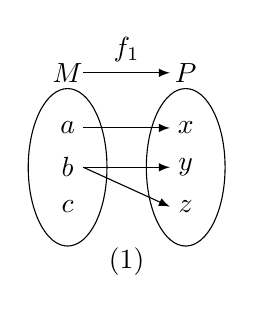
\begin{tikzpicture}[>=latex]
        \draw (0,0) ellipse (0.5 and 1);
        \draw (0,0.5) node {$a$} (0,0) node {$b$} (0,-0.5) node {$c$};
        \draw (1.5,0) ellipse (0.5 and 1);
        \draw (1.5,0.5) node {$x$} (1.5,0) node {$y$} (1.5,-0.5) node {$z$};
        \draw [->] (0.2,0.5) -- (1.3,0.5);
        \draw [->] (0.2,0) -- (1.3,0);
        \draw [->] (0.2,0) -- (1.3,-0.5);
        \draw [->] (0.2,1.2) -- (1.3,1.2);
        \draw (0,1.2) node {$M$} (1.5,1.2) node{$P$};
        \draw (0.75,1.5) node {$f_1$} (0.75,-1.2) node {(1)};
    \end{tikzpicture}
    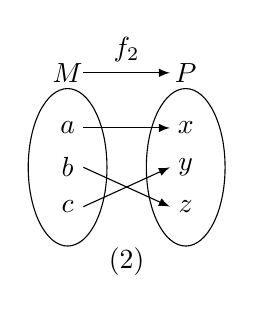
\begin{tikzpicture}[>=latex]
      \draw (0,0) ellipse (0.5 and 1);
      \draw (0,0.5) node {$a$} (0,0) node {$b$} (0,-0.5) node {$c$};
      \draw (1.5,0) ellipse (0.5 and 1);
      \draw (1.5,0.5) node {$x$} (1.5,0) node {$y$} (1.5,-0.5) node {$z$};
      \draw [->] (0.2,0.5) -- (1.3,0.5);
      \draw [->] (0.2,0) -- (1.3,-0.5);
      \draw [->] (0.2,-0.5) -- (1.3,0);
      \draw [->] (0.2,1.2) -- (1.3,1.2);
      \draw (0,1.2) node {$M$} (1.5,1.2) node{$P$};
      \draw (0.75,1.5) node {$f_2$} (0.75,-1.2) node {(2)};
  \end{tikzpicture}
  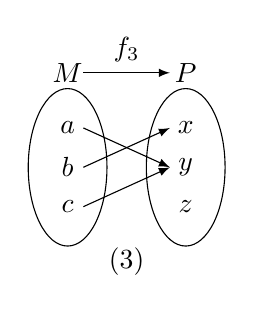
\begin{tikzpicture}[>=latex]
    \draw (0,0) ellipse (0.5 and 1);
    \draw (0,0.5) node {$a$} (0,0) node {$b$} (0,-0.5) node {$c$};
    \draw (1.5,0) ellipse (0.5 and 1);
    \draw (1.5,0.5) node {$x$} (1.5,0) node {$y$} (1.5,-0.5) node {$z$};
    \draw [->] (0.2,0.5) -- (1.3,0);
    \draw [->] (0.2,0) -- (1.3,0.5);
    \draw [->] (0.2,-0.5) -- (1.3,0);
    \draw [->] (0.2,1.2) -- (1.3,1.2);
    \draw (0,1.2) node {$M$} (1.5,1.2) node{$P$};
    \draw (0.75,1.5) node {$f_3$} (0.75,-1.2) node {(3)};
\end{tikzpicture}
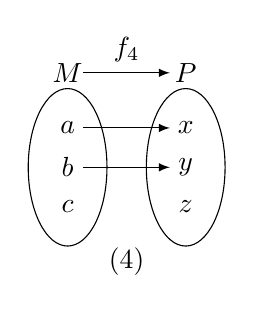
\begin{tikzpicture}[>=latex]
  \draw (0,0) ellipse (0.5 and 1);
  \draw (0,0.5) node {$a$} (0,0) node {$b$} (0,-0.5) node {$c$};
  \draw (1.5,0) ellipse (0.5 and 1);
  \draw (1.5,0.5) node {$x$} (1.5,0) node {$y$} (1.5,-0.5) node {$z$};
  \draw [->] (0.2,0.5) -- (1.3,0.5);
  \draw [->] (0.2,0) -- (1.3,0);
  \draw [->] (0.2,1.2) -- (1.3,1.2);
  \draw (0,1.2) node {$M$} (1.5,1.2) node{$P$};
  \draw (0.75,1.5) node {$f_4$} (0.75,-1.2) node {(4)};
\end{tikzpicture}
\end{center}
\twoch{只有$f_2,f_3$是从$M$到$P$的映射}{只有$f_2,f_4$是从$M$到$P$的映射}{只有$f_3,f_4$是从$M$到$P$的映射}{$f_1,f_2,f_3,f_4$都是从$M$到$P$的映射}


关联目标:

暂未关联目标

答案: 暂无答案

解答或提示: 暂无解答与提示

使用记录:

暂无使用记录


出处: 代数精编第三章函数
\item { (005287)}已知集合$M=\{x|0\le x\le 6\}$, $P=\{0\le y\le 3\}$, 则下列对应关系中, 不能作为从$M$到$P$的映射的是\bracket{20}.
\fourch{$f:x\mapsto y=\dfrac 12x$}{$f:x\mapsto y=\dfrac 13x$}{$f:x\mapsto y=x$}{$f:x\mapsto y=\dfrac 16x$}


关联目标:

暂未关联目标

答案: 暂无答案

解答或提示: 暂无解答与提示

使用记录:

暂无使用记录


出处: 代数精编第三章函数
\item { (005289)}若映射$f:A\to B$的像集是$Y$, 原像的集合是$X$, 则$X$与$A$的关系是\blank{50}, $Y$和$B$的关系是\blank{50}.


关联目标:

暂未关联目标

答案: 暂无答案

解答或提示: 暂无解答与提示

使用记录:

暂无使用记录


出处: 代数精编第三章函数
\item { (005292)}已知$f:x\mapsto y=x^2$是从集合$\mathbf{R}$到集合$M=\{x|x\ge 0\}$的一个映射, 则$M$中的元素$1$在$\mathbf{R}$中的原像是\blank{50}, $M$中的元素$t$($t>0$)在$\mathbf{R}$中的原像是\blank{50}.


关联目标:

暂未关联目标

答案: 暂无答案

解答或提示: 暂无解答与提示

使用记录:

暂无使用记录


出处: 代数精编第三章函数
\item { (005293)}从集合$\{a\}$到$\{b,c\}$的不同映射有\blank{50}个.


关联目标:

暂未关联目标

答案: 暂无答案

解答或提示: 暂无解答与提示

使用记录:

暂无使用记录


出处: 代数精编第三章函数
\item { (005294)}从集合$\{1,2\}$到$\{5,6\}$的不同映射有\blank{50}个.


关联目标:

暂未关联目标

答案: 暂无答案

解答或提示: 暂无解答与提示

使用记录:

暂无使用记录


出处: 代数精编第三章函数
\item { (005295)}已知集合$A=\mathbf{Z}$, $B=\{x|x=2n+1, \ n\in \mathbf{Z}\}$, $C=\mathbf{R}$, 且从$A$到$B$的映射是$x\mapsto 2x-1$, 从$B$到$C$的映射是$x\mapsto \dfrac 1{3x+1}$, 则从$A$到$C$的映射是\blank{50}.


关联目标:

暂未关联目标

答案: 暂无答案

解答或提示: 暂无解答与提示

使用记录:

暂无使用记录


出处: 代数精编第三章函数
\item { (005296)}$f$是集合$X=\{a,b,c\}$到集合$Y=\{d,e\}$的一个映射, 则满足映射条件的``$f$''共有\bracket{20}.
\fourch{$5$个}{$6$个}{$7$个}{$8$个}


关联目标:

暂未关联目标

答案: 暂无答案

解答或提示: 暂无解答与提示

使用记录:

暂无使用记录


出处: 代数精编第三章函数
\item { (005297)}若$f:y=3x+1$是从集合$A=\{1,2,3,k\}$到集合$B=\{4,7,a^4,a^2+3a\}$的一个映射, 求自然数$a,k$的值及集合$A,B$.


关联目标:

暂未关联目标

答案: 暂无答案

解答或提示: 暂无解答与提示

使用记录:

暂无使用记录


出处: 代数精编第三章函数
\item { (005405)}判断命题: $2^{\frac 32}\cdot 2^{\frac 23}=2$是否正确, \blank{50}.


关联目标:

暂未关联目标

答案: 暂无答案

解答或提示: 暂无解答与提示

使用记录:

暂无使用记录


出处: 代数精编第三章函数
\item { (005406)}判断命题: $(\dfrac 18)^{-\frac 12}=-2\sqrt 2$是否正确, \blank{50}.


关联目标:

暂未关联目标

答案: 暂无答案

解答或提示: 暂无解答与提示

使用记录:

暂无使用记录


出处: 代数精编第三章函数
\item { (005407)}判断命题: 若$a\in \mathbf{R}$, 则$(a-1)^0=1$是否正确, \blank{50}.


关联目标:

暂未关联目标

答案: 暂无答案

解答或提示: 暂无解答与提示

使用记录:

暂无使用记录


出处: 代数精编第三章函数
\item { (005408)}判断命题: $a^x+a^y=a^{x+y}$是否正确, \blank{50}.


关联目标:

暂未关联目标

答案: 暂无答案

解答或提示: 暂无解答与提示

使用记录:

暂无使用记录


出处: 代数精编第三章函数
\item { (005409)}判断命题: $\sqrt [3]{-5}=\sqrt [6]{(-5)^2}=\sqrt [6]{25}$是否正确, \blank{50}.


关联目标:

暂未关联目标

答案: 暂无答案

解答或提示: 暂无解答与提示

使用记录:

暂无使用记录


出处: 代数精编第三章函数
\item { (005602)}已知集合$M=\{x|(x+1)^2\le 1\}$, $P=\{y|y=4^x-a\cdot 2^{x+1}+1,\ x\in M,\ \dfrac 34<a\le 1\}$, 且全集$U=\mathbf{R}$, 求$\complement _U(M\cup P)$.


关联目标:

暂未关联目标

答案: 暂无答案

解答或提示: 暂无解答与提示

使用记录:

暂无使用记录


出处: 代数精编第三章函数
\item { (005648)}已知集合$M=\{x,xy,\lg (xy)\}$, $P=\{0,|x|,y\}$, 且满足$M=P$, 求实数$x,y$的值.


关联目标:

暂未关联目标

答案: 暂无答案

解答或提示: 暂无解答与提示

使用记录:

暂无使用记录


出处: 代数精编第三章函数
\item { (005796)}已知集合$A=\{x|x^2-ax+a^2-19=0\}$, $B=\{x|\log_2(x^2-5x+8)=1\}$, $C=\{x|x^2+2x-8=0\}$满足$A\cap B\ne \varnothing$, $A\cap C\ne \varnothing$, 求实数$a$的值.


关联目标:

暂未关联目标

答案: 暂无答案

解答或提示: 暂无解答与提示

使用记录:

暂无使用记录


出处: 代数精编第三章函数
\item { (005816)}已知$f(x)=x^2+ax+b$($a,b$均为实数), 集合$A=\{x|x=f(x) ,x\in \mathbf{R}\}=\{-1,3\}$, $B=\{x|x=f[f(x)],x\in \mathbf{R}\}$, 用列举法求集合.


关联目标:

暂未关联目标

答案: 暂无答案

解答或提示: 暂无解答与提示

使用记录:

暂无使用记录


出处: 代数精编第三章函数
\item { (005817)}已知实数集$\mathbf{R}$的子集$P$满足两个条件: \textcircled{1} $1\notin P$; \textcircled{2} 若实数$a\in P$, 则$\dfrac 1{1-a}\in P$. 求证:\\
(1) 若$2\in P$, 则$P$中必含有其他两个数, 并求出这两个数;\\
(2) 集合$P$不可能是单元素集.


关联目标:

暂未关联目标

答案: 暂无答案

解答或提示: 暂无解答与提示

使用记录:

暂无使用记录


出处: 代数精编第三章函数
\item { (005818)}已知集合$A,B,C$满足$A\cap B=A$, $B\cap C=B$, 求证: $A\subseteq C$.


关联目标:

暂未关联目标

答案: 暂无答案

解答或提示: 暂无解答与提示

使用记录:

暂无使用记录


出处: 代数精编第三章函数
\item { (005819)}已知集合$A=\{x|x=a^2+1,\ a\in \mathbf{N}\}$, $B=\{y|y=b^2-4b+5,\ b\in \mathbf{N}\}$, 求证: $A\subset B$.


关联目标:

暂未关联目标

答案: 暂无答案

解答或提示: 暂无解答与提示

使用记录:

暂无使用记录


出处: 代数精编第三章函数
\item { (005820)}已知集合$A=\{x|x=12a+8b,\ a,b\in \mathbf{Z}\}$, $B=\{x|x=20c+16d,\ c,d\in \mathbf{Z}\}$, 求证: $A=B$.


关联目标:

暂未关联目标

答案: 暂无答案

解答或提示: 暂无解答与提示

使用记录:

暂无使用记录


出处: 代数精编第三章函数
\item { (005824)}已知集合$A=\{(x,y)|\dfrac{y-3}{x-2}=a+1\}$, $B=\{(x,y)|(a^2-1)x+(a-1)y=15\}$满足$A\cap B=\varnothing$, 求实数$a$的值.


关联目标:

暂未关联目标

答案: 暂无答案

解答或提示: 暂无解答与提示

使用记录:

暂无使用记录


出处: 代数精编第三章函数
\item { (005825)}已知集合$A=\{x|x^2-(a+1)^2x+2a^3+2a\le 0,x\in \mathbf{R}\}$, $B=\{x|x^2-3(a+1)x+6a+2\le 0,x\in \mathbf{R}\}$满足$A\subseteq B$, 求实数$a$的取值范围.


关联目标:

暂未关联目标

答案: 暂无答案

解答或提示: 暂无解答与提示

使用记录:

暂无使用记录


出处: 代数精编第三章函数
\item { (005826)}从集合$A=\{1,2,3\}$到集合$M=\{0,1\}$可以建立几个不同的映射?


关联目标:

暂未关联目标

答案: 暂无答案

解答或提示: 暂无解答与提示

使用记录:

暂无使用记录


出处: 代数精编第三章函数
\item { (005827)}从集合$P=\{1,2\}$到集合$Q=\{3,4,5\}$可以建立几个不同的映射?


关联目标:

暂未关联目标

答案: 暂无答案

解答或提示: 暂无解答与提示

使用记录:

暂无使用记录


出处: 代数精编第三章函数
\item { (005837)}已知集合$A=\{x|x^2-5x+4\le 0\}$, $B=\{x|x^2-2ax+a+2\le 0\}$满足$A\supseteq B\ne \varnothing$, 求实数$a$的取值范围.


关联目标:

暂未关联目标

答案: 暂无答案

解答或提示: 暂无解答与提示

使用记录:

暂无使用记录


出处: 代数精编第三章函数
\item { (005850)}已知函数$f(x)=\log_3(x^2-4mx+4m^2+m+\dfrac 1{m-1})$, 集合$M=\{m|m>1,m\in \mathbf{R}\}$.\\
(1) 求证: 当$m\in M$时, $f(x)$的定义域为$x\in \mathbf{R}$; 反之, 若$f(x)$对一切实数$x$都有意义, 则$m\in M$;\\
(2) 当$m\in M$时, 求$f(x)$的最小值;\\
(3) 求证: 对每一个$m\in M$, $f(x)$的最小值都不小于1.


关联目标:

暂未关联目标

答案: 暂无答案

解答或提示: 暂无解答与提示

使用记录:

暂无使用记录


出处: 代数精编第三章函数
\item { (005871)}集合$M=\{\alpha|\alpha =k\cdot 90^\circ , \ k\in \mathbf{N}\}$中各角的终边都在\bracket{20}.
\twoch{$x$轴的正半轴上}{$y$轴的正半轴上}{$x$轴或$y$轴上}{$x$轴正半轴或$y$轴的正半轴上}


关联目标:

暂未关联目标

答案: 暂无答案

解答或提示: 暂无解答与提示

使用记录:

暂无使用记录


出处: 代数精编第四章三角函数
\item { (005876)}集合$M=\{x|x=\dfrac{k\pi}2\pm \dfrac{\pi}4,\ k\in \mathbf{Z}\}$与$P=\{x|x=\dfrac{k\pi}4,\ k\in \mathbf{Z}\}$之间的关系是\bracket{20}.
\fourch{$M\subset P$}{$M\supset P$}{$M=P$}{$M\cap P=\varnothing$}


关联目标:

暂未关联目标

答案: 暂无答案

解答或提示: 暂无解答与提示

使用记录:

暂无使用记录


出处: 代数精编第四章三角函数
\item { (005877)}与$-45^\circ$角终边相同的角的集合是\blank{50}.


关联目标:

暂未关联目标

答案: 暂无答案

解答或提示: 暂无解答与提示

使用记录:

暂无使用记录


出处: 代数精编第四章三角函数
\item { (005879)}终边落在$x$轴负半轴上的角的集合为\blank{50}.


关联目标:

暂未关联目标

答案: 暂无答案

解答或提示: 暂无解答与提示

使用记录:

暂无使用记录


出处: 代数精编第四章三角函数
\item { (005880)}终边落在第一、三象限角平分线上的角的集合为\blank{50}.


关联目标:

暂未关联目标

答案: 暂无答案

解答或提示: 暂无解答与提示

使用记录:

暂无使用记录


出处: 代数精编第四章三角函数
\item { (005882)}若角$\alpha$的终边和函数$y=-|x|$的图像重合, 则$\alpha$的集合是\blank{50}.


关联目标:

暂未关联目标

答案: 暂无答案

解答或提示: 暂无解答与提示

使用记录:

暂无使用记录


出处: 代数精编第四章三角函数
\item { (005891)}若集合$A=\{x|k\pi +\dfrac{\pi}3\le x<k\pi +\dfrac{\pi}2, \ k\in \mathbf{Z}\}$, $B=\{x|4-x^2\ge 0\}$, 则$A\cap B=$\blank{50}.


关联目标:

暂未关联目标

答案: 暂无答案

解答或提示: 暂无解答与提示

使用记录:

暂无使用记录


出处: 代数精编第四章三角函数
\item { (005899)}下列四个命题中, 正确的是\bracket{20}.
\onech{终边相同的角的三角函数值相等}{$\{\alpha|\alpha =k\pi +\dfrac{\pi}6,\ k\in \mathbf{Z}\}\ne \{\beta|\beta =-k\pi +\dfrac{\pi}6,\ k\in \mathbf{Z}\}$}{若$\alpha$是第二象限角, 则$\sin 2\alpha <0$}{第四象限的角可表示为$\{\alpha|2k\pi +\dfrac 32\pi <\alpha <2k\pi ,\ k\in \mathbf{Z}\}$}


关联目标:

暂未关联目标

答案: 暂无答案

解答或提示: 暂无解答与提示

使用记录:

暂无使用记录


出处: 代数精编第四章三角函数
\item { (005902)}直角坐标平面内, 终边过点$(1,-\sqrt 3)$的所有角组成的集合可表示成\blank{50}.


关联目标:

暂未关联目标

答案: 暂无答案

解答或提示: 暂无解答与提示

使用记录:

暂无使用记录


出处: 代数精编第四章三角函数
\item { (005917)}下列四个命题中.能够成立的是\bracket{20}.
\twoch{$\sin \alpha =\dfrac 12$且$\cos \alpha =\dfrac 12$}{$\sin \alpha =\dfrac 13$且$\csc \alpha =2$}{$\sin \alpha =0$且$\cos \alpha =-1$}{$\cos \alpha =\dfrac 12$且$\sec \alpha =-2$}


关联目标:

暂未关联目标

答案: 暂无答案

解答或提示: 暂无解答与提示

使用记录:

暂无使用记录


出处: 代数精编第四章三角函数
\item { (005927)}若$\alpha \in (0,2\pi)$, 则适合$\sqrt {\dfrac{1+\cos \alpha}{1-\cos \alpha}}-\sqrt {\dfrac{1-\cos \alpha}{1+\cos \alpha}}=2\cot \alpha$的角$\alpha$的集合是\bracket{20}.
\twoch{$\{\alpha|0<\alpha <\pi\}$}{$\{\alpha|0<\alpha <\dfrac{\pi}2\pi <\alpha <\dfrac{3\pi}2\}$}{$\{\alpha|0<\alpha <\pi \alpha =\dfrac{3\pi}2\}$}{$\{\alpha|0<\alpha <\dfrac{\pi}2\dfrac{3\pi}2<\alpha <2\pi\}$}


关联目标:

暂未关联目标

答案: 暂无答案

解答或提示: 暂无解答与提示

使用记录:

暂无使用记录


出处: 代数精编第四章三角函数
\item { (006018)}若集合$M=\{\theta|\sin \theta \ge \dfrac 12,0\le \theta \le \pi\}$, $P=\{\theta|\cos \theta \le \dfrac 12,0<\theta \le \pi\}$, 则$M\cap P=$\blank{50}.


关联目标:

暂未关联目标

答案: 暂无答案

解答或提示: 暂无解答与提示

使用记录:

暂无使用记录


出处: 代数精编第四章三角函数
\item { (006358)}若$AD$是Rt$\triangle ABC$斜边$BC$上的高, 则下列命题不成立的是\bracket{20}.
\fourch{$\sin B=\sqrt {\dfrac{CD}{BC}}$}{$\cos B=\sqrt {\dfrac{BD}{BC}}$}{$\tan B=\sqrt {\dfrac{BD}{CD}}$}{$\cot B=\sqrt {\dfrac{BD\cdot BC}{AC}}$}


关联目标:

暂未关联目标

答案: 暂无答案

解答或提示: 暂无解答与提示

使用记录:

暂无使用记录


出处: 代数精编第五章三角恒等式与解三角形
\item { (006526)}满足不等式$2\arccos x-\arccos (-x)>0$的$x$的取值集合为\blank{50}.


关联目标:

暂未关联目标

答案: 暂无答案

解答或提示: 暂无解答与提示

使用记录:

暂无使用记录


出处: 代数精编第六章反三角与三角方程
\item { (006527)}满足不等式$\arccos 3x<\arccos (2-5x)$的$x$的取值集合为\blank{50}.


关联目标:

暂未关联目标

答案: 暂无答案

解答或提示: 暂无解答与提示

使用记录:

暂无使用记录


出处: 代数精编第六章反三角与三角方程
\item { (006528)}满足不等式$\arccos (2x^2-1)<\arccos x$的$x$的取值集合为\blank{50}.


关联目标:

暂未关联目标

答案: 暂无答案

解答或提示: 暂无解答与提示

使用记录:

暂无使用记录


出处: 代数精编第六章反三角与三角方程
\item { (006529)}满足不等式$\arccos x>\arcsin x$的$x$的取值集合为\blank{50}.


关联目标:

暂未关联目标

答案: 暂无答案

解答或提示: 暂无解答与提示

使用记录:

暂无使用记录


出处: 代数精编第六章反三角与三角方程
\item { (006532)}下列四个命题中正确的是\bracket{20}.
\twoch{若$\sin f(x)$是奇函数, 则$f(x)$是奇函数}{若$\cos f(x)$是奇函数, 则$f(x)$是奇函数}{若$\arcsin f(x)$是奇函数, 则$f(x)$是奇函数}{若$\arccos f(x)$是奇函数, 则$f(x)$是奇函数}


关联目标:

暂未关联目标

答案: 暂无答案

解答或提示: 暂无解答与提示

使用记录:

暂无使用记录


出处: 代数精编第六章反三角与三角方程
\item { (006918)}利用数学归纳法证明``对任意偶数$n$, $a^n-b^n$能被$a+b$整除''时, 其第二步论证, 应该是\bracket{20}.
\onech{假设$n=k$时命题成立, 再证$n=k+1$时命题也成立}{假设$n=2k$时命题成立, 再证$n=2k+1$时命题也成立}{假设$n=k$时命题成立, 再证$n=k+2$时命题也成立}{假设$n=2k$时命题成立, 再证$n=2(k+1)$时命题也成立}


关联目标:

暂未关联目标

答案: 暂无答案

解答或提示: 暂无解答与提示

使用记录:

暂无使用记录


出处: 代数精编第七章数列
\item { (006921)}利用数学归纳法证明不等式``$\sqrt {n^2+n}<n+1$''时, 由``假设$n=k$时命题成立''到``当$n=k+1$时'', 正确的步骤是\bracket{20}.
\onech{$\sqrt {(k+1)^2+(k+1)}=\sqrt {k^2+3k+2}<\sqrt {k^2+4k+4}=k+2$}{$\sqrt {(k+1)^2+(k+1)}=\sqrt {k^2+3k+2}=\sqrt {(k+2)^2-(k+2)}<k+2$}{$\sqrt {(k+1)^2+(k+1)}=\sqrt {k^2+3k+2}<\sqrt {(k+2)^2}=k+2$}{$\sqrt {(k+1)^2+(k+1)}=\sqrt {k^2+3k+2}=\sqrt {(k^2+k)+2k+2}<\sqrt {(k+1)^2+2k+2}=\sqrt {(k+2)^2-1}<\sqrt {(k+2)^2}=k+2$}


关联目标:

暂未关联目标

答案: 暂无答案

解答或提示: 暂无解答与提示

使用记录:

暂无使用记录


出处: 代数精编第七章数列
\item { (006996)}下列结论中, 正确的是\bracket{20}.
\onech{复平面内, 原点是实轴与虚轴的公共点}{实数的共轭复数一定是实数, 虚数的共轭复数一定是虚数}{复数集$\mathbf{C}$与复平面内所有向量所组成的集合是一一对应的}{若使得实数$x$对应于纯虚数$x\mathrm{i}$, 则实数集$\mathbf{R}$与纯虚数集是一一对应的}


关联目标:

暂未关联目标

答案: 暂无答案

解答或提示: 暂无解答与提示

使用记录:

暂无使用记录


出处: 代数精编第八章复数
\item { (006999)}已知集合$M=\{1,2,(m^2-3m-1)+(m^2-5m+6)\mathrm{i},m\in \mathbf{R}\}$, $N=\{-1,3\}$满足$M\cap N\ne \varnothing$, 则$m$等于\bracket{20}.
\fourch{$0$或$3$}{$-1$或$3$}{$-1$或$6$}{$3$}


关联目标:

暂未关联目标

答案: 暂无答案

解答或提示: 暂无解答与提示

使用记录:

暂无使用记录


出处: 代数精编第八章复数
\item { (007002)}判断命题的真假: $x_1+y_1\mathrm{i}=x_2+y_2\mathrm{i}$的充要条件是$x_1=x_2$, 且$y_1=y_2$.\blank{50}.


关联目标:

暂未关联目标

答案: 暂无答案

解答或提示: 暂无解答与提示

使用记录:

暂无使用记录


出处: 代数精编第八章复数
\item { (007003)}判断命题的真假: 任意两个复数都不能比较大小.\blank{50}.


关联目标:

暂未关联目标

答案: 暂无答案

解答或提示: 暂无解答与提示

使用记录:

暂无使用记录


出处: 代数精编第八章复数
\item { (007004)}判断命题的真假: 若$x,y\in \mathbf{R}$, 且$x=y$, 则$(x-y)+(x+y)\mathrm{i}$是纯虚数.\blank{50}.


关联目标:

暂未关联目标

答案: 暂无答案

解答或提示: 暂无解答与提示

使用记录:

暂无使用记录


出处: 代数精编第八章复数
\item { (007024)}根据条件, 在复平面内画出复数对应点的集合所表示的图形: $1\le|\mathrm{Re}(z)|\le 2$($\mathrm{Re}(z)$表示$z$的实部).


关联目标:

暂未关联目标

答案: 暂无答案

解答或提示: 暂无解答与提示

使用记录:

暂无使用记录


出处: 代数精编第八章复数
\item { (007025)}根据条件, 在复平面内画出复数对应点的集合所表示的图形: $1\le|z|\le 2$且$\mathrm{Im}(z)<0$($\mathrm{Im}(z)$表示$z$的虚部).


关联目标:

暂未关联目标

答案: 暂无答案

解答或提示: 暂无解答与提示

使用记录:

暂无使用记录


出处: 代数精编第八章复数
\item { (007026)}已知两个复数集$M=\{z|z=t+(1-t^2)\mathrm{i}, t\in \mathbf{R}\}$及$N=\{z|z=2\cos \theta +(\lambda +3\sin \theta)\mathrm{i},\lambda \in \mathbf{R},\theta \in \mathbf{R}\}$的交集为非空集合, 求$\lambda$的取值范围.


关联目标:

暂未关联目标

答案: 暂无答案

解答或提示: 暂无解答与提示

使用记录:

暂无使用记录


出处: 代数精编第八章复数
\item { (007060)}已知两个复数集合$A=\{z||z-2|\le 2\}$, $B=\{z|z=\dfrac{z_1}2\mathrm{i}+b, \ z_1\in A, \ b\in \mathbf{R}\}$.\\
(1) 当$b=0$时, 求集合$B$所对应的区域;\\
(2) 当$A\cap B=\varnothing$时, 求$b$的取值范围;\\
(3) 若复数$z_1=1+2a\mathrm{i}$, $z_2=a+\mathrm{i}$($a\in \mathbf{R}$), 集合$A=\{z||z-z_1|\le \sqrt 2\}$, $B=\{z||z-z_2|\le 2\sqrt 2\}$满足$A\cap B=\varnothing$, 求$a$的取值范围.


关联目标:

暂未关联目标

答案: 暂无答案

解答或提示: 暂无解答与提示

使用记录:

暂无使用记录


出处: 代数精编第八章复数
\item { (007373)}若集合$M=\{-1,1,2\}$, 且$a,b,r\in M$, 则$(x-a)^2+(y-b)^2=r^2$所表示的不同圆共有\blank{50}个.


关联目标:

暂未关联目标

答案: 暂无答案

解答或提示: 暂无解答与提示

使用记录:

暂无使用记录


出处: 代数精编第九章排列组合
\item { (007384)}若集合$A=\{a_1,a_2,a_3,a_4,a_5\}$, $B=\{b_1,b_2,b_3\}$, 则从集合$A$到$B$可建立\blank{50}个不同的映射, 从集合$B$到集合$A$可建立\blank{50}个不同的映射.


关联目标:

暂未关联目标

答案: 暂无答案

解答或提示: 暂无解答与提示

使用记录:

暂无使用记录


出处: 代数精编第九章排列组合
\item { (007408)}已知集合$M=\{a_1,a_2,a_3\}$, $P=\{b_1,b_2,b_3,b_4,b_5,b_6\}$, 若$M$中的不同元素对应到$P$中的不同像, 则这样的映射个数共有\bracket{20}.
\fourch{$3$}{$20$}{$64$}{$120$}


关联目标:

暂未关联目标

答案: 暂无答案

解答或提示: 暂无解答与提示

使用记录:

暂无使用记录


出处: 代数精编第九章排列组合
\item { (007446)}从集合$P=\{1,2,3\}$, $Q=\{1,4,5,6\}$这两个集合中各取一个元素作为平面直角坐标系中点的坐标, 能确定的不同点的个数是\bracket{20}.
\fourch{$11$}{$12$}{$23$}{$24$}


关联目标:

暂未关联目标

答案: 暂无答案

解答或提示: 暂无解答与提示

使用记录:

暂无使用记录


出处: 代数精编第九章排列组合
\item { (007497)}从集合$M=\{1,2,3,4,5\}$到集合$N=\{a,b,c\}$的映射, 要求集合$N$中的元素在集合$M$中都有原像, 这样的映射有几种?


关联目标:

暂未关联目标

答案: 暂无答案

解答或提示: 暂无解答与提示

使用记录:

暂无使用记录


出处: 代数精编第九章排列组合
\item { (007503)}从集合$\{51,52,53,\cdots ,99\}$中任选$2$个数, 使这$2$个数的和为偶数, 有多少种不同的选法?


关联目标:

暂未关联目标

答案: 暂无答案

解答或提示: 暂无解答与提示

使用记录:

暂无使用记录


出处: 代数精编第九章排列组合
\item { (007524)}已知集合$A$和集合$B$各含有$12$个元素, $A\cap B$含有$4$个元素, 试求同时满足下列两个条件的集合$C$的个数:\\
(1) $C\subset (A\cup B)$, 且$C$中含有$3$个元素;\\
(2) $C\cap A\ne \varnothing$.


关联目标:

暂未关联目标

答案: 暂无答案

解答或提示: 暂无解答与提示

使用记录:

暂无使用记录


出处: 代数精编第九章排列组合
\item { (007579)}若集合$P=\{\text{所有小于}1993\text{的正奇数}\}$, 则$P$的非空真子集的个数是\bracket{20}.
\fourch{$2^{996}$}{$2^{996}-2$}{$2^{996}-1$}{$2^{995}$}


关联目标:

暂未关联目标

答案: 暂无答案

解答或提示: 暂无解答与提示

使用记录:

暂无使用记录


出处: 代数精编第九章排列组合
\item { (007624)}设含有$10$个元素的集合的全部子集为$S$, 其中由$3$个元素组成的子集数为$T$, 则$\dfrac TS$的值为\blank{50}.


关联目标:

暂未关联目标

答案: 暂无答案

解答或提示: 暂无解答与提示

使用记录:

暂无使用记录


出处: 代数精编第九章排列组合
\item { (007634)}求满足$\{a,b\}\subset A\subseteq \{a,b,c,d,e,f,g\}$的集合$A$的个数.


关联目标:

暂未关联目标

答案: 暂无答案

解答或提示: 暂无解答与提示

使用记录:

暂无使用记录


出处: 代数精编第九章排列组合
\item { (007635)}设集合$A=\{0,2,5,7,9\}$, 从集合$A$中任取两个元素相乘, 它们的积组成集合$B$, 求集合$B$的子集的个数.


关联目标:

暂未关联目标

答案: 暂无答案

解答或提示: 暂无解答与提示

使用记录:

暂无使用记录


出处: 代数精编第九章排列组合
\item { (007669)}设集合$P=\{a_1,a_2,\cdots ,a_n\}$, 在$P$中取子集$A_1$, $A_2$, $A_3$, 使$A_1\cap A_2\cap A_3=\varnothing$, 这样子集的集合$\{A_1,A_2,A_3\}$共有多少个?


关联目标:

暂未关联目标

答案: 暂无答案

解答或提示: 暂无解答与提示

使用记录:

暂无使用记录


出处: 代数精编第九章排列组合
\item { (007674)}设自然数$N=\{1,2,3,\cdots\}$的子集中含有$4$个元素的子集的个数记为$m$, 且这$m$个集合中所有元素之和为$\dfrac 1{12}\mathrm{P}_{100}^5$, 求$m$.


关联目标:

暂未关联目标

答案: 暂无答案

解答或提示: 暂无解答与提示

使用记录:

暂无使用记录


出处: 代数精编第九章排列组合
\item { (007680)}用列举法表示下列集合:\\
(1) 十二生肖名称的集合;\\
(2) $10$以内的素数组成的集合;\\
(3) $\{y|y=x^2-1, \ -1<x<3, \ x\in \mathbf{Z}\}$.


关联目标:

暂未关联目标

答案: 暂无答案

解答或提示: 暂无解答与提示

使用记录:

暂无使用记录


出处: 二期课改练习册高一第一学期
\item { (007681)}用描述法表示下列集合:\\
(1) 被$3$除余数等于$1$的整数的集合;\\
(2) 比$1$大又比$10$小的实数组成的集合;\\
(3) 平面直角坐标系内横轴上的点的坐标组成的集合.


关联目标:

暂未关联目标

答案: 暂无答案

解答或提示: 暂无解答与提示

使用记录:

暂无使用记录


出处: 二期课改练习册高一第一学期
\item { (007683)}集合$\{(x,y)|xy\ge 0, \ x\in \mathbf{R}, \ y\in \mathbf{R}\}$是指\bracket{20}.
\twoch{第一象限内的所有点}{第三象限内的所有点}{第一象限和第三象限内的所有点}{不在第二象限、第四象限内的所有点}


关联目标:

暂未关联目标

答案: 暂无答案

解答或提示: 暂无解答与提示

使用记录:

暂无使用记录


出处: 二期课改练习册高一第一学期
\item { (007684)}用适当的方法表示下列集合:\\
(1) 方程$x^2-2=0$的实数解组成的集合;\\
(2) 两直线$y=2x+1$和$y=x-2$的交点组成的集合.


关联目标:

暂未关联目标

答案: 暂无答案

解答或提示: 暂无解答与提示

使用记录:

暂无使用记录


出处: 二期课改练习册高一第一学期
\item { (007685)}已知集合$A=\{2,(a+1)^2,a^2+3a+3\}$, 且$1\in A$, 求实数$a$的值.


关联目标:

暂未关联目标

答案: 暂无答案

解答或提示: 暂无解答与提示

使用记录:

暂无使用记录


出处: 二期课改练习册高一第一学期
\item { (007686)}指出下列各集合之间存在的关系:\\
(1) $A=\{x|x^2-2x+1=0\}$, $B=\{x|x^2-1=0\}$;\\
(2) $A=\{1,2,4,8\}$, $B=\{x|x\text{是}8\text{的正约数}\}$.


关联目标:

暂未关联目标

答案: 暂无答案

解答或提示: 暂无解答与提示

使用记录:

暂无使用记录


出处: 二期课改练习册高一第一学期
\item { (007688)}若集合$A=\{x|x=2n+1, \ n\in \mathbf{Z}\}$, 集合$B=\{x|x=4n-1, \ n\in \mathbf{Z}\}$, 则$A$、$B$的关系是\bracket{20}.
\fourch{$A\subseteq B$}{$A=B$}{$A\subsetneqq B$}{$B\subsetneqq A$}


关联目标:

暂未关联目标

答案: 暂无答案

解答或提示: 暂无解答与提示

使用记录:

暂无使用记录


出处: 二期课改练习册高一第一学期
\item { (007689)}已知集合$A=\{1\}$, 集合$B=\{x|x^2-3x+a=0\}$, 且$A\subsetneqq B$, 求实数$a$的值.


关联目标:

暂未关联目标

答案: 暂无答案

解答或提示: 暂无解答与提示

使用记录:

暂无使用记录


出处: 二期课改练习册高一第一学期
\item { (007690)}已知集合$A=\{x,y\}$, 集合$B=\{2x,2x^2\}$, 且$A=B$, 求集合$A$.


关联目标:

暂未关联目标

答案: 暂无答案

解答或提示: 暂无解答与提示

使用记录:

暂无使用记录


出处: 二期课改练习册高一第一学期
\item { (007691)}已知集合$S=\{1,2\}$, 集合$T=\{x|ax^2-3x+2=0\}$, 且$S=T$, 求实数$a$的值.


关联目标:

暂未关联目标

答案: 暂无答案

解答或提示: 暂无解答与提示

使用记录:

暂无使用记录


出处: 二期课改练习册高一第一学期
\item { (007692)}已知$a$是常数, 集合$M=\{x|x^2+x-6=0\}$, 集合$N=\{y|ay+2=0\}$, 且$N\subseteq M$, 求实数$a$的值.


关联目标:

暂未关联目标

答案: 暂无答案

解答或提示: 暂无解答与提示

使用记录:

暂无使用记录


出处: 二期课改练习册高一第一学期
\item { (007693)}已知所有菱形组成的集合为$A$, 所有矩形组成的集合为$B$, 求$A\cap B$.


关联目标:

暂未关联目标

答案: 暂无答案

解答或提示: 暂无解答与提示

使用记录:

暂无使用记录


出处: 二期课改练习册高一第一学期
\item { (007694)}已知集合$A=\{x|x\le 7\}$, 集合$B=\{x|x<2\}$, 集合$C=\{x|x>5\}$, 求$A\cap B$, $A\cap C$, $A\cap (B\cap C)$.


关联目标:

暂未关联目标

答案: 暂无答案

解答或提示: 暂无解答与提示

使用记录:

暂无使用记录


出处: 二期课改练习册高一第一学期
\item { (007695)}已知集合$A=\{(x,y)|y=-x+1\}$, 集合$B=\{(x,y)|y=x^2-1\}$, 求$A\cap B$.


关联目标:

暂未关联目标

答案: 暂无答案

解答或提示: 暂无解答与提示

使用记录:

暂无使用记录


出处: 二期课改练习册高一第一学期
\item { (007696)}已知集合$A=\{x|x\text{是锐角三角形}\}$, 集合$B=\{x|x\text{是钝角三角形}\}$, 求$A\cap B$, $A\cup B$.


关联目标:

暂未关联目标

答案: 暂无答案

解答或提示: 暂无解答与提示

使用记录:

暂无使用记录


出处: 二期课改练习册高一第一学期
\item { (007697)}已知集合$A=\{x|x^2+px+15=0\}$, 集合$B=\{x|x^2-5x+q=0\}$, 且$A\cap B=\{3\}$, 求$p$、$q$的值和$A\cup B$.


关联目标:

暂未关联目标

答案: 暂无答案

解答或提示: 暂无解答与提示

使用记录:

暂无使用记录


出处: 二期课改练习册高一第一学期
\item { (007698)}已知集合$A=\{x|x\le 1\}$, 集合 $B=\{x|x\ge a\}$, 且$A\cup B=\mathbf{R}$, 求$a$的取值范围.


关联目标:

暂未关联目标

答案: 暂无答案

解答或提示: 暂无解答与提示

使用记录:

暂无使用记录


出处: 二期课改练习册高一第一学期
\item { (007699)}已知集合$A=\{x|x\text{是平行四边形}\}$, 集合$U=\{x|x\text{是至少有一组对边平行的四边形}\}$, 求$\complement _UA$.


关联目标:

暂未关联目标

答案: 暂无答案

解答或提示: 暂无解答与提示

使用记录:

暂无使用记录


出处: 二期课改练习册高一第一学期
\item { (007700)}设$U=\mathbf{R}$, 集合$A=\{x|4-x>2x+1\}$, 求$\complement _UA$.


关联目标:

暂未关联目标

答案: 暂无答案

解答或提示: 暂无解答与提示

使用记录:

暂无使用记录


出处: 二期课改练习册高一第一学期
\item { (007701)}已知集合$U=\{x|0<x\le 10, \ x\in \mathbf{N}\}$, 集合$A=\{1,2,4,5,9\}$, 集合$B=\{4,6,7,8,10\}$, 求$\complement _UA$, $\complement _UB$, $\complement _UA\cup \complement _UB$, $\complement _UA\cap \complement _UB$, $\complement _U(A\cap B)$, $\complement _U(A\cup B)$, 并指出其中相等的集合.


关联目标:

暂未关联目标

答案: 暂无答案

解答或提示: 暂无解答与提示

使用记录:

暂无使用记录


出处: 二期课改练习册高一第一学期
\item { (007703)}已知集合$A=\{1,4,x\}$, 集合$B=\{1,x^2\}$, 且$A\cup B=A$, 求$x$的值及集合$A$、$B$.


关联目标:

暂未关联目标

答案: 暂无答案

解答或提示: 暂无解答与提示

使用记录:

暂无使用记录


出处: 二期课改练习册高一第一学期
\item { (007704)}已知集合$A=\{x|-2\le x\le 4\}$, 集合$B=\{x|-3<x<2\}$, 集合$C=\{x|-3\le x<0\}$, 求$A\cup B$, $(A\cap B)\cup C$, $(A\cup C)\cap (B\cup C)$.


关联目标:

暂未关联目标

答案: 暂无答案

解答或提示: 暂无解答与提示

使用记录:

暂无使用记录


出处: 二期课改练习册高一第一学期
\item { (007705)}已知集合$U=\{x|x\ge 2\}$, 集合$A=\{y|3\le y<4\}$, 集合$B=\{z|2\le z<5\}$, 求$\complement _UA\cap B$, $\complement _UB\cup A$.


关联目标:

暂未关联目标

答案: 暂无答案

解答或提示: 暂无解答与提示

使用记录:

暂无使用记录


出处: 二期课改练习册高一第一学期
\item { (007706)}已知集合$U=\{a,b,c,d,e,f\}$, 集合$A=\{a,b,c,d\}$, $A\cap B=\{a\}$, $\complement _U(A\cup B)=\{f\}$, 求集合$B$.


关联目标:

暂未关联目标

答案: 暂无答案

解答或提示: 暂无解答与提示

使用记录:

暂无使用记录


出处: 二期课改练习册高一第一学期
\item { (007707)}判断下列语句是否为命题, 并在相应的括号内填入``是''或``否''.\\
(1) 正方形是四边形; \blank{20}\\
(2) $0$是自然数吗; \blank{20}\\
(3) 交集和并集; \blank{20}\\
(4) $3<\pi$. \blank{20}


关联目标:

暂未关联目标

答案: 暂无答案

解答或提示: 暂无解答与提示

使用记录:

暂无使用记录


出处: 二期课改练习册高一第一学期
\item { (007708)}判断下列命题的真假, 并在相应的括号内填入``真命题''或``假命题''.\\
(1) 如果$a$、$b$都是奇数, 那么$a+b$是偶数; \blank{20}\\
(2) 一组对边平行且两对角线相等的四边形是平行四边形; \blank{20}\\
(3) 如果$|a|<2$, 那么$a<2$; \blank{20}\\
(4) 如果$A\cap B=A$, 那么$A\cup B=B$. \blank{20}


关联目标:

暂未关联目标

答案: 暂无答案

解答或提示: 暂无解答与提示

使用记录:

暂无使用记录


出处: 二期课改练习册高一第一学期
\item { (007710)}已知命题$A$: 如果$x<3$, 那么$x<5$; 命题$B$: 如果$x\ge 3$, 那么$x\ge 5$; 命题$C$: 如果$x\ge 5$, 那么$x\ge 3$.填写各命题之间的关系:
$A$与$B$互为\blank{20}命题, $B$与$C$互为\blank{20}命题, $C$与$A$互为\blank{20}命题.


关联目标:

暂未关联目标

答案: 暂无答案

解答或提示: 暂无解答与提示

使用记录:

暂无使用记录


出处: 二期课改练习册高一第一学期
\item { (007711)}写出命题``在$\triangle ABC$中, 如果$\angle C>\angle B$, 那么$AB>AC$''的逆命题、否命题和逆否命题, 并判断其真假.


关联目标:

暂未关联目标

答案: 暂无答案

解答或提示: 暂无解答与提示

使用记录:

暂无使用记录


出处: 二期课改练习册高一第一学期
\item { (007712)}写出命题``如果$\alpha$, 那么$\beta$''的逆命题、否命题和逆否命题.


关联目标:

暂未关联目标

答案: 暂无答案

解答或提示: 暂无解答与提示

使用记录:

暂无使用记录


出处: 二期课改练习册高一第一学期
\item { (007713)}写出命题``已知$a$、$b$、$c$是实数, 如果$ac<0$, 那么$ax^2+bx+c=0(a\ne 0)$有实数根''的逆命题.否命题和逆否命题, 并判断其真假.


关联目标:

暂未关联目标

答案: 暂无答案

解答或提示: 暂无解答与提示

使用记录:

暂无使用记录


出处: 二期课改练习册高一第一学期
\item { (007714)}命题``若$x\ne 3$且$x\ne 4$, 则$x^2-7x+12\ne 0$''的逆否命题是\bracket{20}.
\twoch{若$x^2-7x+12=0$, 则$x=3$或$x=4$}{若$x^2-7x+12=0$, 则$x\ne 3$或$x\ne 4$}{若$x^2-7x+12\ne 0$, 则$x\ne 3$且$x\ne 4$}{若$x^2-7x+12=0$, 则$x=3$且$x=4$}


关联目标:

暂未关联目标

答案: 暂无答案

解答或提示: 暂无解答与提示

使用记录:

暂无使用记录


出处: 二期课改练习册高一第一学期
\item { (007715)}如果命题$A$的逆命题是$B$, 命题$A$的否命题是$C$, 那么命题$B$是命题$C$的\bracket{20}.
\fourch{逆命题}{否命题}{逆否命题}{以上都不正确}


关联目标:

暂未关联目标

答案: 暂无答案

解答或提示: 暂无解答与提示

使用记录:

暂无使用记录


出处: 二期课改练习册高一第一学期
\item { (007716)}试判断命题$A$: ``在$\triangle ABC$中, $BC^2=AC^2+AB^2$''与命题$B$: ``$\triangle ABC$是直角三角形''是否为等价命题, 并说明理由.


关联目标:

暂未关联目标

答案: 暂无答案

解答或提示: 暂无解答与提示

使用记录:

暂无使用记录


出处: 二期课改练习册高一第一学期
\item { (007717)}试判断命题$A$: ``三角形任意两边之和大于第三边''与命题$B$: ``三角形任意两边之差小于第三边''是否为等价命题, 并说明理由.


关联目标:

暂未关联目标

答案: 暂无答案

解答或提示: 暂无解答与提示

使用记录:

暂无使用记录


出处: 二期课改练习册高一第一学期
\item { (007719)}判断下列命题的真假, 并在相应的横线上填入``真命题''或``假命题''.\\
(1) 若$A\cap B\ne \varnothing$, $B\subsetneqq C$, 则$A\cap C\ne \varnothing$\blank{20};\\
(2) 方程$(a+1)x+b=0$($a$、$b\in \mathbf{R}$)的解为$x=-\dfrac b{a+1}$\blank{20};\\
(3)若命题$\alpha$、$\beta$、$\gamma$满足$\alpha \Rightarrow \beta$, $\beta \Rightarrow \gamma$, $\gamma \Rightarrow \alpha$, 则$\alpha \Leftrightarrow \gamma$\blank{20}.


关联目标:

暂未关联目标

答案: 暂无答案

解答或提示: 暂无解答与提示

使用记录:

暂无使用记录


出处: 二期课改练习册高一第一学期
\item { (007720)}若$\alpha$: $\{2\}\subsetneqq B\subseteq \{2,3,4\}$, $\beta :B=\{2,4\}$, 则$\alpha$与$\beta$的推出关系是\bracket{20}.
\fourch{$\alpha \Rightarrow \beta$}{$\beta \Rightarrow \alpha$}{$\alpha \Leftrightarrow \beta$}{$\alpha \not\Rightarrow \beta$且$\beta \not\Rightarrow \alpha$}
(2)由命题甲成立, 可推出命题乙不成立, 下列说法一定正确的是\bracket{20}.
\twoch{命题甲不成立, 可推出命题乙成立}{命题甲不成立, 可推出命题乙不成立}{命题乙成立, 可推出命题甲成立}{命题乙成立, 可推出命题甲不成立}


关联目标:

暂未关联目标

答案: 暂无答案

解答或提示: 暂无解答与提示

使用记录:

暂无使用记录


出处: 二期课改练习册高一第一学期
\item { (007721)}已知一个命题的否命题是``两组对边分别相等的四边形是平行四边形'', 试写出原命题的逆命题, 并判断原命题的真假.


关联目标:

暂未关联目标

答案: 暂无答案

解答或提示: 暂无解答与提示

使用记录:

暂无使用记录


出处: 二期课改练习册高一第一学期
\item { (007722)}已知一个命题的逆命题是``若实数$a$、$b$满足$a=1$且$b=2$, 则$a+b<4$'', 试写出原命题的否命题, 并判断原命题的真假.


关联目标:

暂未关联目标

答案: 暂无答案

解答或提示: 暂无解答与提示

使用记录:

暂无使用记录


出处: 二期课改练习册高一第一学期
\item { (007723)}类比$A\subseteq B\Leftrightarrow A\cap B=A$, 试再写出两个等价命题:\\
$A\subseteq B\Leftrightarrow$\blank{50};\\
$A\subseteq B\Leftrightarrow$\blank{50}.


关联目标:

暂未关联目标

答案: 暂无答案

解答或提示: 暂无解答与提示

使用记录:

暂无使用记录


出处: 二期课改练习册高一第一学期
\item { (007724)}下列各题中命题$P$是命题$Q$的什么条件?\\
(1) $P$: 四边形的四条边相等, $Q$: 四边形是正方形;\\
(2) $P$: $\triangle ABC\cong \triangle DEF$,	$Q$: $\triangle ABC$的面积$=\triangle DEF$的面积;\\
(3) $P$: $x$是$2$的倍数, $Q$: $x$是$6$的倍数;\\
(4) $P$: 两个三角形全等, $Q$: 两个三角形的两角和一边对应相等.


关联目标:

暂未关联目标

答案: 暂无答案

解答或提示: 暂无解答与提示

使用记录:

暂无使用记录


出处: 二期课改练习册高一第一学期
\item { (007730)}有下列四组命题:
\textcircled{1} $P$: 集合$A\subseteq B$, $B\subseteq C$, $C\subseteq A$, 		$Q$: 集合$A=B=C$;
\textcircled{2} $P$: $A\cap B=A\cap C$, 					$Q$: $B=C$;
\textcircled{3} $P$: $(x-2)(x-3)=0$, 				$Q$: $\dfrac{x-2}{x-3}=0$;
\textcircled{4} $P$: 抛物线$y=ax^2+bx+c(a\ne 0)$过原点, $Q$: $c=0$.
其中$P$是$Q$的充要条件的有\bracket{20}.
\fourch{\textcircled{1} 、\textcircled{2} }{\textcircled{1} 、\textcircled{4} }{\textcircled{2} 、\textcircled{3} }{\textcircled{2} 、\textcircled{4}}


关联目标:

暂未关联目标

答案: 暂无答案

解答或提示: 暂无解答与提示

使用记录:

暂无使用记录


出处: 二期课改练习册高一第一学期
\item { (007733)}命题``$x\in M$或$x\in P$''是命题``$x\in M\cap P$''的什么条件?


关联目标:

暂未关联目标

答案: 暂无答案

解答或提示: 暂无解答与提示

使用记录:

暂无使用记录


出处: 二期课改练习册高一第一学期
\item { (007734)}写出命题``$x>3$''的一个充分条件和一个必要条件.


关联目标:

暂未关联目标

答案: 暂无答案

解答或提示: 暂无解答与提示

使用记录:

暂无使用记录


出处: 二期课改练习册高一第一学期
\item { (007737)}填空:
已知集合$A=\{a|a$具有性质$p\}$, $B=\{b|b$具有性质$q\}$.\\
(1) 若$A\subseteq B$, 则$p$是$q$的\blank{50}条件;\\
(2) 若$A\supseteq B$, 则$p$是$q$的\blank{50}条件;\\
(3) 若$A=B$, 则$p$是$q$的\blank{50}条件.


关联目标:

暂未关联目标

答案: 暂无答案

解答或提示: 暂无解答与提示

使用记录:

暂无使用记录


出处: 二期课改练习册高一第一学期
\item { (007738)}试用子集与推出关系来判断命题$A$是命题$B$的什么条件.\\
(1) $A$: 该平面图形是四边形, $B$: 该平面图形是梯形;\\
(2) $A$: $x=2$, $B$: $(x-5)(x-2)=0$;\\
(3) $A$: $x^2=y^2$, $B$: $x=y$;\\
(4) $A$: $a=2$, $B$: $a\le 2$.


关联目标:

暂未关联目标

答案: 暂无答案

解答或提示: 暂无解答与提示

使用记录:

暂无使用记录


出处: 二期课改练习册高一第一学期
\item { (007739)}如果命题$p$: $m<-3$, 命题$q$: 方程$x^2-x-m=0$无实数根, 那么$p$是$q$的什么条件?


关联目标:

暂未关联目标

答案: 暂无答案

解答或提示: 暂无解答与提示

使用记录:

暂无使用记录


出处: 二期课改练习册高一第一学期
\item { (007740)}已知命题$\alpha$: $2\le x<4$, 命题$\beta$: $3m-1\le x\le -m$, 且$\alpha$是$\beta$的充分条件, 求实数$m$的取值范围.


关联目标:

暂未关联目标

答案: 暂无答案

解答或提示: 暂无解答与提示

使用记录:

暂无使用记录


出处: 二期课改练习册高一第一学期
\item { (007741)}如果命题$p$: $A\subseteq B$, 命题$q$: $A\subsetneqq B$, 那么$p$是$q$的什么条件?


关联目标:

暂未关联目标

答案: 暂无答案

解答或提示: 暂无解答与提示

使用记录:

暂无使用记录


出处: 二期课改练习册高一第一学期
\item { (007743)}下列命题中正确的是\bracket{20}.
\twoch{自然数集$\mathbf{N}$中最小的数是$1$}{空集是任何集合的真子集}{如果$A\subseteq B$, 且$A\ne B$, 那么$A$是$B$的真子集}{$\{y|y=x+3,\ x\in \mathbf{N}\}$中的最小值是$4$}


关联目标:

暂未关联目标

答案: 暂无答案

解答或提示: 暂无解答与提示

使用记录:

暂无使用记录


出处: 二期课改练习册高一第一学期
\item { (007745)}已知$I$是全集.若$M$、$P$、$S$是$I$的$3$个子集, 则图中阴影部分所表示的集合是\bracket{20}.
\begin{center}
    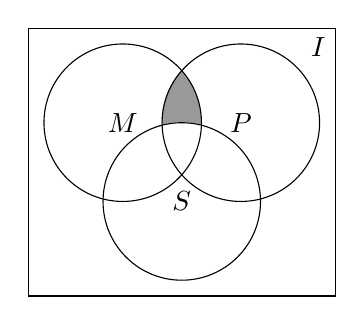
\begin{tikzpicture}
        \begin{scope}
            \clip (0,0) circle (1);
            \filldraw [gray!80] (1.5,0) circle (1);
        \end{scope}
        \filldraw [white] (0.75,-1) circle (1);
        \draw (0,0) circle (1) node {$M$};
        \draw (1.5,0) circle (1) node {$P$};
        \draw (0.75,-1) circle (1) node {$S$};
        \draw (-1.2,-2.2) rectangle (2.7,1.2) node [below left] {$I$};
    \end{tikzpicture}
\end{center}
\fourch{$(M\cap P)\cap S$}{$(M\cap P)\cup S$}{$(M\cap P)\cap \complement _IS$}{$(M\cap P)\cup \complement _IS$}


关联目标:

暂未关联目标

答案: 暂无答案

解答或提示: 暂无解答与提示

使用记录:

暂无使用记录


出处: 二期课改练习册高一第一学期
\item { (007746)}若命题$p$: $x^2-5x+6=0$, 命题$q$: $x=2$, 则$p$是$q$的\blank{50}条件。


关联目标:

暂未关联目标

答案: 暂无答案

解答或提示: 暂无解答与提示

使用记录:

暂无使用记录


出处: 二期课改练习册高一第一学期
\item { (007750)}若方程$x^2+px+4=0$的解集为$A$, 方程$x^2+x+q=0$的解集为$B$, 且$A\cap B=\{4\}$, 则集合$A\cup B$的所有子集是\blank{50}.


关联目标:

暂未关联目标

答案: 暂无答案

解答或提示: 暂无解答与提示

使用记录:

暂无使用记录


出处: 二期课改练习册高一第一学期
\item { (007752)}已知集合$A=\{x|-2<x\le 1\}$, 集合$B=\{x|x\ge 1x<-2\}$, 求$A\cup B$, $A\cap B$.


关联目标:

暂未关联目标

答案: 暂无答案

解答或提示: 暂无解答与提示

使用记录:

暂无使用记录


出处: 二期课改练习册高一第一学期
\item { (007753)}已知集合$A=\{x|-1<x<1$或$x\ge 3\}$, 集合$U=\{x|x\ge 2x<1\}$, 求$\complement _UA$.


关联目标:

暂未关联目标

答案: 暂无答案

解答或提示: 暂无解答与提示

使用记录:

暂无使用记录


出处: 二期课改练习册高一第一学期
\item { (007754)}写出命题: 若$x>1$, 则$x>0$的逆命题、否命题、逆否命题, 并指出哪些是真命题.


关联目标:

暂未关联目标

答案: 暂无答案

解答或提示: 暂无解答与提示

使用记录:

暂无使用记录


出处: 二期课改练习册高一第一学期
\item { (007755)}已知集合$A=\{x|x^2+px+q=0\}$, 集合$B=\{x|x^2-x+r=0\}$, 且$A\cap B=\{-1\}$, $A\cup B=\{-1,2\}$, 求$p$、$q$、$r$的值.


关联目标:

暂未关联目标

答案: 暂无答案

解答或提示: 暂无解答与提示

使用记录:

暂无使用记录


出处: 二期课改练习册高一第一学期
\item { (007756)}已知全集$U=\mathbf{R}$, 集合$A=\{x|x\le a-1\}$, 集合$B=\{x|x>a+2\}$, 集合$C=\{x|x<0$或$x\ge 4\}$.若$\complement _U(A\cup B)\subseteq C$, 求实数$a$的取值范围.


关联目标:

暂未关联目标

答案: 暂无答案

解答或提示: 暂无解答与提示

使用记录:

暂无使用记录


出处: 二期课改练习册高一第一学期
\item { (007757)}若集合$M=\{a|a=x+\sqrt 2y,\ x,y\in \mathbf{Q}\}$, 则下列结论正确的是\bracket{20}.
\fourch{$M\subseteq \mathbf{Q}$}{$M=\mathbf{Q}$}{$M\supsetneqq \mathbf{Q}$}{$M\subsetneqq \mathbf{Q}$}


关联目标:

暂未关联目标

答案: 暂无答案

解答或提示: 暂无解答与提示

使用记录:

暂无使用记录


出处: 二期课改练习册高一第一学期
\item { (007760)}已知集合$P=\{x|-2\le x\le 5\}$, 集合$Q=\{x|k+1\le x\le 2k-1\}$, 且$Q\subseteq P$, 求实数$k$的取值范围.


关联目标:

暂未关联目标

答案: 暂无答案

解答或提示: 暂无解答与提示

使用记录:

暂无使用记录


出处: 二期课改练习册高一第一学期
\item { (007761)}已知集合$A=\{x|(a-1)x^2+3x-2=0\}$, 是否存在这样的实数$a$, 使得集合$A$有且仅有两个子集? 若存在, 求出实数$a$的值及对应的两个子集;若不存在.请说明理由.


关联目标:

暂未关联目标

答案: 暂无答案

解答或提示: 暂无解答与提示

使用记录:

暂无使用记录


出处: 二期课改练习册高一第一学期
\item { (007793)}已知集合$U=\mathbf{R}$, 且集合$A=\{x|x^2-16<0\}$, 集合$B=\{x|x^2-4x+3\ge 0\}$, 求:\\
(1) $A\cap B$;\\
(2) $A\cup B$;\\
(3) $\complement _U(A\cap B)$;\\
(4) $\complement _UA\cup \complement _UB$.


关联目标:

暂未关联目标

答案: 暂无答案

解答或提示: 暂无解答与提示

使用记录:

暂无使用记录


出处: 二期课改练习册高一第一学期
\item { (007919)}已知集合$A=\{x|1\le x\le 4\}$, $f(x)=x^2+px+q$和$g(x)=x+\dfrac 4x$是定义在$A$上的函数, 且在$x_0$处同时取到最小值, 并满足$f(x_0)=g(x_0)$, 求$f(x)$在$A$上的最大值.


关联目标:

暂未关联目标

答案: 暂无答案

解答或提示: 暂无解答与提示

使用记录:

暂无使用记录


出处: 二期课改练习册高一第一学期
\item { (007961)}已知集合$M=\{y|y=2^x,\ x\in \mathbf{R}\}$, 集合$N=\{y|y=x^2,\ x\in \mathbf{R}\}$, 求$M\cap N$.


关联目标:

暂未关联目标

答案: 暂无答案

解答或提示: 暂无解答与提示

使用记录:

暂无使用记录


出处: 二期课改练习册高一第一学期
\item { (007980)}若集合$A=\{y|y=x^2+2c+3\}$, 集合$B=\{y|y=x+\dfrac 4x\}$, 则$A\cup B=$\blank{50}.


关联目标:

暂未关联目标

答案: 暂无答案

解答或提示: 暂无解答与提示

使用记录:

暂无使用记录


出处: 二期课改练习册高一第一学期
\item { (007981)}已知$x,y\in \mathbf{R}$, 集合$\alpha =\{(x,y)|xy\ge 0\}$, 集合$\beta =\{(x,y)||x+y|=|x|+|y|\}$, 用推出关系表示$\alpha$与$\beta$的关系\blank{50}.


关联目标:

暂未关联目标

答案: 暂无答案

解答或提示: 暂无解答与提示

使用记录:

暂无使用记录


出处: 二期课改练习册高一第一学期
\item { (007985)}若集合$A=\{x|0.1<\dfrac 1x<0.3,\ x\in \mathbf{N}\}$, 集合$B=\{x||x|\le 5,\ x\in \mathbf{Z}\}$, 则$A\cup B$中的元素个数是\bracket{20}.
\fourch{$11$}{$13$}{$15$}{$17$}


关联目标:

暂未关联目标

答案: 暂无答案

解答或提示: 暂无解答与提示

使用记录:

暂无使用记录


出处: 二期课改练习册高一第一学期
\item { (007988)}已知集合$A=\{x|3x^2+x-2\ge 0,\  x\in \mathbf{R}\}$, 集合$B=\{x|\dfrac{4x-3}{x-3}>0,\ x\in \mathbf{R}\}$, 求$A\cap B$.


关联目标:

暂未关联目标

答案: 暂无答案

解答或提示: 暂无解答与提示

使用记录:

暂无使用记录


出处: 二期课改练习册高一第一学期
\item { (007990)}已知集合$A=(-2,-1)\cup (0,+\infty)$, 集合$B=\{x|x^2+ax+b\le 0\}$, 且$A\cap B=(0,2]$, $A\cup B=(-2,+\infty)$, 求实数$a$、$b$的值.


关联目标:

暂未关联目标

答案: 暂无答案

解答或提示: 暂无解答与提示

使用记录:

暂无使用记录


出处: 二期课改练习册高一第一学期
\item { (007995)}已知集合$A=\{x||x-a|<2\}$, 集合$B=\{x|\dfrac{2x-1}{x-2}<1\}$, 且$A\subseteq B$, 求实数$a$的取值范围.


关联目标:

暂未关联目标

答案: 暂无答案

解答或提示: 暂无解答与提示

使用记录:

暂无使用记录


出处: 二期课改练习册高一第一学期
\item { (007996)}已知全集$U=\mathbf{R}$, 集合$A=\{x|x^2+px+12=0\}$, 集合$B=\{x|x-5x-q=0\}$, 满足$(\complement _UA)\cap B=\{2\}$.求实数$p$与$q$的值.


关联目标:

暂未关联目标

答案: 暂无答案

解答或提示: 暂无解答与提示

使用记录:

暂无使用记录


出处: 二期课改练习册高一第一学期
\item { (008098)}判断命题``若函数$y=f(x)$与$y=f^{-1}(x)$的图像有公共点, 则公共点必在直线$y=x$上''的真假, 并说明理由.


关联目标:

暂未关联目标

答案: 暂无答案

解答或提示: 暂无解答与提示

使用记录:

暂无使用记录


出处: 二期课改练习册高一第二学期
\item { (008107)}写出终边在$x$轴与$y$轴的夹角的平分线上的角的集合(分别用角度制和弧度制来表示).


关联目标:

暂未关联目标

答案: 暂无答案

解答或提示: 暂无解答与提示

使用记录:

暂无使用记录


出处: 二期课改练习册高一第二学期
\item { (008108)}在平面直角坐标系中, 用阴影部分表示集合: $\{\alpha|30^\circ+k\cdot 360^\circ\le \alpha \le 60^\circ+k\cdot 360^\circ, \ k\in \mathbf{Z}\}$.


关联目标:

暂未关联目标

答案: 暂无答案

解答或提示: 暂无解答与提示

使用记录:

暂无使用记录


出处: 二期课改练习册高一第二学期
\item { (008109)}第一象限角的集合是\blank{50}.


关联目标:

暂未关联目标

答案: 暂无答案

解答或提示: 暂无解答与提示

使用记录:

暂无使用记录


出处: 二期课改练习册高一第二学期
\item { (008110)}终边在坐标轴上的角的集合是\blank{50}.


关联目标:

暂未关联目标

答案: 暂无答案

解答或提示: 暂无解答与提示

使用记录:

暂无使用记录


出处: 二期课改练习册高一第二学期
\item { (008111)}写出与$60^\circ$终边相同的角的集合$S$, 并写出$S$中适合不等式$-360^\circ\le \alpha <720^\circ$的元素$\alpha$.


关联目标:

暂未关联目标

答案: 暂无答案

解答或提示: 暂无解答与提示

使用记录:

暂无使用记录


出处: 二期课改练习册高一第二学期
\item { (008112)}写出与$-21^\circ$终边相同的角的集合$S$, 并写出$S$中适合不等式$-360^\circ\le \alpha <720^\circ$的元素$\alpha$.


关联目标:

暂未关联目标

答案: 暂无答案

解答或提示: 暂无解答与提示

使用记录:

暂无使用记录


出处: 二期课改练习册高一第二学期
\item { (008245)}求函数$y=2-\sin x$取得最大值和最小值的$x$的集合, 并求出其最大值和最小值.


关联目标:

暂未关联目标

答案: 暂无答案

解答或提示: 暂无解答与提示

使用记录:

暂无使用记录


出处: 二期课改练习册高一第二学期
\item { (008246)}求函数$y=3\sin (2x-\dfrac{\pi}3)$取得最大值和最小值的$x$的集合, 并求出其最大值和最小值.


关联目标:

暂未关联目标

答案: 暂无答案

解答或提示: 暂无解答与提示

使用记录:

暂无使用记录


出处: 二期课改练习册高一第二学期
\item { (008260)}已知$0\le x\le 2\pi$, 求适合下列条件的角$x$的集合:\\
(1) 角$x$的正弦函数、余弦函数都是增函数;\\
(2) 角$x$的正弦函数是减函数, 余弦函数是增函数.


关联目标:

暂未关联目标

答案: 暂无答案

解答或提示: 暂无解答与提示

使用记录:

暂无使用记录


出处: 二期课改练习册高一第二学期
\item { (008264)}求函数$y=\sqrt 3\sin x+\cos x$取得最大值和最小值的$x$的集合, 并求出其最大值和最小值.


关联目标:

暂未关联目标

答案: 暂无答案

解答或提示: 暂无解答与提示

使用记录:

暂无使用记录


出处: 二期课改练习册高一第二学期
\item { (008265)}求函数$y=2+|\cos x|$取得最大值和最小值的$x$的集合, 并求出其最大值和最小值.


关联目标:

暂未关联目标

答案: 暂无答案

解答或提示: 暂无解答与提示

使用记录:

暂无使用记录


出处: 二期课改练习册高一第二学期
\item { (008278)}已知$0\le x\le 2\pi$, 求使角$x$的正弦函数、正切函数都是增函数的角$x$的集合.


关联目标:

暂未关联目标

答案: 暂无答案

解答或提示: 暂无解答与提示

使用记录:

暂无使用记录


出处: 二期课改练习册高一第二学期
\item { (008279)}已知$0\le x\le 2\pi$, 求使角$x$的余弦函数是减函数, 正切函数是增函数的角$x$的集合.


关联目标:

暂未关联目标

答案: 暂无答案

解答或提示: 暂无解答与提示

使用记录:

暂无使用记录


出处: 二期课改练习册高一第二学期
\item { (008345)}已知函数$y=\dfrac 12a\cos x(\cos x+\sqrt 3\sin x)+1$, 且函数的图像过点$P(\dfrac{\pi}6,\dfrac 74)$.\\
(1) 求函数的解析式;\\
(2) 当$y$取最大值时, 求自变量$x$的集合.


关联目标:

暂未关联目标

答案: 暂无答案

解答或提示: 暂无解答与提示

使用记录:

暂无使用记录


出处: 二期课改练习册高一第二学期
\item { (008357)}已知下列四个命题:\\
\textcircled{1} 函数$y=\sin (\dfrac{5\pi}2-2x)$是偶函数;
\textcircled{2} 函数$y=\tan x$在定义域内是增函数;
\textcircled{3} 函数$y=\tan (ax-1)$的最小正周期是$\dfrac{\pi}a$;
\textcircled{4} $x=\dfrac{\pi}8$是函数$y=\sin (2x+\dfrac{\pi}4)$图像的一条对称轴方程.
其中正确命题的序号是\blank{50}.


关联目标:

暂未关联目标

答案: 暂无答案

解答或提示: 暂无解答与提示

使用记录:

暂无使用记录


出处: 二期课改练习册高一第二学期
\item { (008483)}选择题:
下列四个命题中, 正确的是\bracket{20}.
\twoch{若$\displaystyle\lim_{n\to\infty}a_n^2=A^2$, 则$\displaystyle\lim_{n\to\infty}a_n=A$}{若$a_n>0$, $\displaystyle\lim_{n\to\infty}a_n=A$, 则$A>0$}{若$\displaystyle\lim_{n\to\infty}a_n=A$, 则$\displaystyle\lim_{n\to\infty}a_n^2=A^2$}{若$\displaystyle\lim_{n\to\infty}a_n=A$, 则$\displaystyle\lim_{n\to\infty}na_n=nA$}


关联目标:

暂未关联目标

答案: 暂无答案

解答或提示: 暂无解答与提示

使用记录:

暂无使用记录


出处: 二期课改练习册高二第一学期
\item { (008498)}下列命题中, 正确的是\bracket{20}.
\onech{若$\displaystyle\lim_{n\to\infty}(a_n\cdot b_n)=a\ne 0$, 则$\displaystyle\lim_{n\to\infty}a_n\ne 0$且$\displaystyle\lim_{n\to\infty}b_n\ne 0$}{若$\displaystyle\lim_{n\to\infty}(a_n\cdot b_n)=0$, 则$\displaystyle\lim_{n\to\infty}a_n=0$或$\displaystyle\lim_{n\to\infty}b_n=0$}{若无穷数列$\{a_n\}$有极限, 且它的前$n$项和为$S_n$, 则$\displaystyle\lim_{n\to\infty}S_n=\displaystyle\lim_{n\to\infty}a_1+\displaystyle\lim_{n\to\infty}a_2+\cdots$ $+\displaystyle\lim_{n\to\infty}a_n$}{若无穷数列$\{a_n\}$有极限$A$, 则$\displaystyle\lim_{n\to\infty}a_n=\displaystyle\lim_{n\to\infty}a_{n+1}$}


关联目标:

暂未关联目标

答案: 暂无答案

解答或提示: 暂无解答与提示

使用记录:

暂无使用记录


出处: 二期课改练习册高二第一学期
\item { (008523)}某个命题与正整数有关, 如果当$n=k(k\in \mathbf{N}^*)$时命题成立, 那么可以推得当$n=k+1$时命题也成立.现在已知当$n=5$时该命题不成立, 所以该命题在\bracket{20}.
\fourch{$n=6$时成立}{$n=6$时不成立}{$n=4$时成立}{$n=4$时不成立}


关联目标:

暂未关联目标

答案: 暂无答案

解答或提示: 暂无解答与提示

使用记录:

暂无使用记录


出处: 二期课改练习册高二第一学期
\item { (008717)}现有以下四个命题:
\textcircled{1} 时间、速度、加速度都是向量;
\textcircled{2} 向量的模是一个正实数;
\textcircled{3} 所有的单位向量都相等;
\textcircled{4} 零向量与任意非零向量平行.
其中真命题的个数是\bracket{20}.
\fourch{$1$}{$2$}{$3$}{$4$}


关联目标:

暂未关联目标

答案: 暂无答案

解答或提示: 暂无解答与提示

使用记录:

暂无使用记录


出处: 二期课改练习册高二第一学期
\item { (008718)}判断题(下列命题中, 如果命题是真命题, 那么在横线上填入``$\checkmark$''; 如果命题是假命题, 那么在横线上填入``$\times$''):\\
(1) 长度相等的向量都相等.\blank{20};\\
(2) 若$\overrightarrow a=\overrightarrow b$, $\overrightarrow b=\overrightarrow c$, 则$\overrightarrow a=\overrightarrow c$.\blank{20};\\
(3) 若四边形$ABCD$是平行四边形, 则$\overrightarrow{AB}=\overrightarrow{CD}$.\blank{20};\\
(4) 若$\overrightarrow{AB}=\overrightarrow{DC}$, 则$|\overrightarrow{AB}|=|\overrightarrow{CD}|$且直线$AB\parallel CD$.\blank{20}.


关联目标:

暂未关联目标

答案: 暂无答案

解答或提示: 暂无解答与提示

使用记录:

暂无使用记录


出处: 二期课改练习册高二第一学期
\item { (008721)}如图, $B,C$是线段$AD$的三等分点, 分别以图中各点为起点和终点的非零向量组成集合$T$, 试写出集合$T$中所有的元素.
\begin{center}
    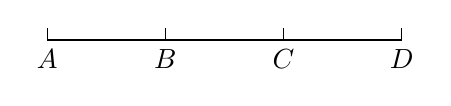
\begin{tikzpicture}[scale = 1.5]
        \draw (0,0) -- (3,0);
        \draw (0,0.1) -- (0,0) node [below] {$A$};
        \draw (1,0.1) -- (1,0) node [below] {$B$};
        \draw (2,0.1) -- (2,0) node [below] {$C$};
        \draw (3,0.1) -- (3,0) node [below] {$D$};
    \end{tikzpicture}
\end{center}


关联目标:

暂未关联目标

答案: 暂无答案

解答或提示: 暂无解答与提示

使用记录:

暂无使用记录


出处: 二期课改练习册高二第一学期
\item { (008789)}已知集合$A=\{(x,y)|x-y-1=0,\ x,y\in \mathbf{R}\}$, 集合$B=\{(x,y)|ax-y+2=0,\ x,y\in \mathbf{R}\}$, 且$A\cap B=\varnothing$, 求实数$a$的值.


关联目标:

暂未关联目标

答案: 暂无答案

解答或提示: 暂无解答与提示

使用记录:

暂无使用记录


出处: 二期课改练习册高二第二学期
\item { (008938)}下列四个命题中, 正确的是\bracket{20}.
\onech{到两坐标轴距离相等的点的轨迹方程为$y=x$}{两相交直线$y=\dfrac{\sqrt 3}3x$与$y=\sqrt 3x$的夹角平分线的方程为$y=x$}{$\triangle ABC$的三个顶点的坐标分别为$A(1,1)$、$B(3,1)$、$C(1,3)$, $BC$边上的中线方程为$y=x$}{与两顶点$A(-1,0)$、$B(1,0)$的连线的夹角为$90^{\circ }$的动点的轨迹方程为$x^2+y^2=1$}


关联目标:

暂未关联目标

答案: 暂无答案

解答或提示: 暂无解答与提示

使用记录:

暂无使用记录


出处: 二期课改练习册高二第二学期
\item { (008962)}命题: 椭圆$\dfrac{x^2}{25}+\dfrac{y^2}9=1$与双曲线$\dfrac{x^2}{11}-\dfrac{y^2}5=1$的焦距相等.试将此命题推广到一般情形, 使已知命题成为推广后命题的一个特例:\blank{50}.


关联目标:

暂未关联目标

答案: 暂无答案

解答或提示: 暂无解答与提示

使用记录:

暂无使用记录


出处: 二期课改练习册高二第二学期
\item { (008968)}(1) 已知直线$l$: $4x-y-1=0$与抛物线$x^2=2y$交于$A(x_A,y_A)$、$B(x_B,y_B)$两点, 直线$l$与$x$轴相交于点$C(x_C,0)$, 求证: $\dfrac 1{x_A}+\dfrac 1{x_B}=\dfrac 1{x_C}$;\\
(2) 试将第(1)题中的命题加以推广, 使得第(1)题中的命题是推广后得到的命题的特例, 并证明推广后得到的命题正确.


关联目标:

暂未关联目标

答案: 暂无答案

解答或提示: 暂无解答与提示

使用记录:

暂无使用记录


出处: 二期课改练习册高二第二学期
\item { (008970)}用集合的关系符号表示复数集$\mathbf{C}$、实数集$\mathbf{R}$、有理数集$\mathbf{Q}$、整数集$\mathbf{Z}$和自然数集$\mathbf{N}$的关系为\blank{50}.


关联目标:

暂未关联目标

答案: 暂无答案

解答或提示: 暂无解答与提示

使用记录:

暂无使用记录


出处: 二期课改练习册高二第二学期
\item { (008984)}判断题: (下列命题中, 是真命题的在横线上填入``$\checkmark$''; 是假命题的在横线上填入``$\times$'')
(1) 表示实数的点都在实轴上, 表示纯虚数的点都在虚轴上.\blank{20};\\
(2) 表示虚数的点都落在四个象限内.\blank{20};\\
(3) 复数的模表示该复数在复平面上所对应的点到原点的距离.\blank{20}.


关联目标:

暂未关联目标

答案: 暂无答案

解答或提示: 暂无解答与提示

使用记录:

暂无使用记录


出处: 二期课改练习册高二第二学期
\item { (008987)}已知复数$z$分别满足下列条件, 复数$z$在复平面上对应点$Z$, 画出点$Z$的集合对应的图形.\\
(1) $|z|=3$;\\ 
(2) $|z|<3$;\\
(3) $2\le|z|\le 5$.


关联目标:

暂未关联目标

答案: 暂无答案

解答或提示: 暂无解答与提示

使用记录:

暂无使用记录


出处: 二期课改练习册高二第二学期
\item { (008996)}下列四个命题:
\textcircled{1} 复数$z$与它的共轭复数$\overline  z$不能比较大小, 但它们的模相等;
\textcircled{2} 互为共轭的两个复数的和为实数, 而它们的差为纯虚数;
\textcircled{3} 若复数$z$的共轭复数是$-z$, 则$z$一定是纯虚数;
\textcircled{4} 若复数$z$的共轭复数是它自身, 则$z$一定是实数.
其中正确命题的序号是\blank{50}.


关联目标:

暂未关联目标

答案: 暂无答案

解答或提示: 暂无解答与提示

使用记录:

暂无使用记录


出处: 二期课改练习册高二第二学期
\item { (009003)}已知$|z-2|=|z-2\mathrm{i}|$, 写出复数$z$在复平面上所对应的点$Z$的集合是什么图形.


关联目标:

暂未关联目标

答案: 暂无答案

解答或提示: 暂无解答与提示

使用记录:

暂无使用记录


出处: 二期课改练习册高二第二学期
\item { (009029)}判断题: (下列命题中, 是真命题的在横线上填入``$\checkmark$''; 是假命题的在横线上填入``$\times$'')\\
(1) 在复数范围内, 方程$ax^2+bx+c=0$($a,b,c\in \mathbf{R}$, $a\ne 0$)总有两个根.\blank{20};\\
(2) 若$1+2\mathrm{i}$是方程$x^2+px+q=0$的一个根, 则这个方程的另一个根是$1-2\mathrm{i}$.\blank{20};\\
(3) 若方程$x^2+px+q=0$有两个共轭虚根, 则$pq$均为实数.\blank{20}.


关联目标:

暂未关联目标

答案: 暂无答案

解答或提示: 暂无解答与提示

使用记录:

暂无使用记录


出处: 二期课改练习册高二第二学期
\item { (009059)}已知复数$z$分别满足下列条件, 写出它在复平面上对应的点$Z$的集合分别是什么图形.\\
(1) $|z-\mathrm{i}|=|z-3|$;\\ 
(2) $|z-1+\mathrm{i}|=|z-\mathrm{i}-3|$;\\
(3) $z\overline z+z+\overline z=0$.


关联目标:

暂未关联目标

答案: 暂无答案

解答或提示: 暂无解答与提示

使用记录:

暂无使用记录


出处: 二期课改练习册高二第二学期
\item { (009060)}已知集合$A=\{z|z=2a-1+a^2\mathrm{i},\ a\in \mathbf{R}\}$. 当实数$a$变化时, 说明集合$A$中元素在复平面上所对应的点的轨迹表示何种曲线.


关联目标:

暂未关联目标

答案: 暂无答案

解答或提示: 暂无解答与提示

使用记录:

暂无使用记录


出处: 二期课改练习册高二第二学期
\item { (009062)}复数集是实数集的扩充, 因此复数在保留实数的一些性质(如$(a+b)^2=a^2+2ab+b^2$等)的同时, 也使得实数的一些性质(如有序性等)在复数集上不能成立.试写出若干个在实数范围内成立, 而在复数范围内不成立的命题.


关联目标:

暂未关联目标

答案: 暂无答案

解答或提示: 暂无解答与提示

使用记录:

暂无使用记录


出处: 二期课改练习册高二第二学期
\item { (009064)}在复数范围内, 下列命题正确的是\bracket{20}.
\twoch{若$z$是非零复数, 则$z-\overline z$一定是纯虚数}{若复数$z$满足$z^2=-|z^2|$, 则$z$是纯虚数}{若$z_1^2+z_2^2=0$, 则$z_1=0$且$z_2=0$}{若$z_1,z_2$为两个复数, 则$z_1\overline  z_2+\overline  z_1z_2$一定是实数}


关联目标:

暂未关联目标

答案: 暂无答案

解答或提示: 暂无解答与提示

使用记录:

暂无使用记录


出处: 二期课改练习册高二第二学期
\item { (009078)}集合$\{z|z=\mathrm{i}^n+\dfrac 1{\mathrm{i}^n}, \ n\in \mathbf{N}^*\}$用列举法可表示为\blank{50}.


关联目标:

暂未关联目标

答案: 暂无答案

解答或提示: 暂无解答与提示

使用记录:

暂无使用记录


出处: 二期课改练习册高二第二学期
\item { (009111)}用集合语言表示下列语句并画图表示:\\
(1) 点$M$是平面$\alpha$与平面$\beta$的公共点;\\
(2) 平面$\alpha$与平面$\beta$没有公共点, 且直线$l$与平面$\alpha$和平面$\beta$分别交于点$A$和点$B$;\\
(3) 平面$\alpha$与平面$\beta$交于直线$l$, 且直线$l$与平面$\gamma$没有公共点.


关联目标:

暂未关联目标

答案: 暂无答案

解答或提示: 暂无解答与提示

使用记录:

暂无使用记录


出处: 二期课改练习册高三
\item { (009116)}用集合语言表示下列语句并画图:
如果平面$\alpha$与平面$\beta$交于直线$l$, 平面$\alpha$与平面$\gamma$交于直线$n$, 平面$\beta$与平面$\gamma$交于直线$n$, 且直线$l$与直线$m$平行, 那么直线$l$、$m$、$n$两两平行.


关联目标:

暂未关联目标

答案: 暂无答案

解答或提示: 暂无解答与提示

使用记录:

暂无使用记录


出处: 二期课改练习册高三
\item { (009137)}判断题: (下列命题中, 是真命题的在横线上填入``$\checkmark$''; 是假命题的在横线上填入``$\times$'')\\
(1) 一条直线在平面内的射影是一条直线.\blank{20};\\
(2) 在平面内射影是直线的图形一定是直线.\blank{20};\\
(3) 如果两条线段在同一平面内的射影长相等, 那么这两条线段的长相等.\blank{20};\\
(4) 如果两条斜线与平面所成的角相等, 那么这两条斜线互相平行.\blank{20}.


关联目标:

暂未关联目标

答案: 暂无答案

解答或提示: 暂无解答与提示

使用记录:

暂无使用记录


出处: 二期课改练习册高三
\item { (009151)}判断题: (下列命题中, 是真命题的在横线上填入``$\checkmark$''; 是假命题的在横线上填入``$\times$'')\\
(1) 二面角指的是两个平面相交所组成的图形.\blank{20};\\
(2) 二面角指的是一个平面绕这个平面内的一条直线旋转所组成的图形.\blank{20};\\
(3) 二面角指的是以一个平面内的一条直线为边界的一个半平面与这个平面所组成的图形.\blank{20};\\
(4) 二面角指的是从一条直线出发的两个半平面所组成的图形.\blank{20}.


关联目标:

暂未关联目标

答案: 暂无答案

解答或提示: 暂无解答与提示

使用记录:

暂无使用记录


出处: 二期课改练习册高三
\item { (009159)}下列命题中不正确的是\bracket{20}.
\onech{如果平面$\alpha$与平面$\beta$平行, 那么平面$\alpha$内任一直线平行于平面$\beta$}{如果一个平面内任何一条直线都平行于另一个平面, 那么这两个平面平行}{如果一条直线$m$与两个平面$\alpha$、$\beta$所成的角相等, 那么$\alpha \parallel\beta$}{分别在两个平行平面内的两条直线只能是平行直线或异面直线}


关联目标:

暂未关联目标

答案: 暂无答案

解答或提示: 暂无解答与提示

使用记录:

暂无使用记录


出处: 二期课改练习册高三
\item { (009165)}画出下列点、直线和平面之间的位置关系图, 并用集合符号表示.\\
(1) 直线$l$在平面$\alpha$上, 点$M$在平面$\alpha$上, 但不在直线$l$上;\\
(2) 平面$\alpha$与平面$\beta$交于直线$l$. 直线$a$与平面$\alpha$、平面$\beta$都没有公共点.


关联目标:

暂未关联目标

答案: 暂无答案

解答或提示: 暂无解答与提示

使用记录:

暂无使用记录


出处: 二期课改练习册高三
\item { (009166)}将下列集合符号表述改为自然语言表述, 并判断它们是否正确.\\
(1) $A\in \beta$, $B\in \beta \Rightarrow AB\not\in \beta$;\\
(2) $A\in \alpha$, $B\in \alpha$, $C\in AB\Rightarrow C\in \alpha$.


关联目标:

暂未关联目标

答案: 暂无答案

解答或提示: 暂无解答与提示

使用记录:

暂无使用记录


出处: 二期课改练习册高三
\item { (009192)}四棱柱集合$A$、平行六面体集合$B$、长方体集合$C$、正方体集合$D$之间有怎样的包含关系? 用文氏图表示出来.


关联目标:

暂未关联目标

答案: 暂无答案

解答或提示: 暂无解答与提示

使用记录:

暂无使用记录


出处: 二期课改练习册高三
\item { (009226)}现有以下三个命题: \textcircled{1} 底面是平行四边形的四棱柱是平行六面体; \textcircled{2} 底面是矩形的平行六面体是长方体; \textcircled{3} 直四棱柱是直平行六面体. 其中真命题的序号是\blank{50}.


关联目标:

暂未关联目标

答案: 暂无答案

解答或提示: 暂无解答与提示

使用记录:

暂无使用记录


出处: 二期课改练习册高三
\item { (009256)}已知集合$M=\{-3,-2,-1,0,1,2\}$, 点$P(a,b) $在直角坐标平面上, 且$a, b\in M$.\\
(1) 平面上共有多少个满足条件的点$P$?\\
(2) 有多少个点$P$在第二象限内?\\
(3) 有多少个点$P$不在直线$y=x$上?


关联目标:

暂未关联目标

答案: 暂无答案

解答或提示: 暂无解答与提示

使用记录:

暂无使用记录


出处: 二期课改练习册高三
\item { (009273)}已知抛物线方程为$y=ax^2+bx+c$, 集合$M=\{-2,-1,0,1,2,3,4\}$, $a,b,c\in M$, 且$a,b,c$两两不相等, 满足条件的抛物线中, 过原点的抛物线有多少条?


关联目标:

暂未关联目标

答案: 暂无答案

解答或提示: 暂无解答与提示

使用记录:

暂无使用记录


出处: 二期课改练习册高三
\item { (009296)}(1) 计算$\mathrm{C}_2^0+\mathrm{C}_2^1+\mathrm{C}_2^2$;\\
(2) 计算: $\mathrm{C}_3^0+\mathrm{C}_3^1+\mathrm{C}_3^2+\mathrm{C}_3^3$;\\
(3) 猜想$\mathrm{C}_n^0+\mathrm{C}_n^1+\mathrm{C}_n^2+\cdots +\mathrm{C}_n^{n-1}+\mathrm{C}_n^n(n\in \mathbf{N}^*) $的值, 并证明你的结果;\\
(4) 你能否利用第(3)题来求一个集合的子集的个数? 为什么?


关联目标:

暂未关联目标

答案: 暂无答案

解答或提示: 暂无解答与提示

使用记录:

暂无使用记录


出处: 二期课改练习册高三
\item { (009301)}已知集合$AB$都含有$12$个元素, $A\cap B$含有$4$个元素, 集合$C$含有$3$个元素, 且$C\subsetneqq A\cup B,C\cap B\ne \varnothing$, 求满足条件的集合$C$的个数.


关联目标:

暂未关联目标

答案: 暂无答案

解答或提示: 暂无解答与提示

使用记录:

暂无使用记录


出处: 二期课改练习册高三
\item { (009392)}用集合语言表示下列语句, 并画图表示: 点$P$在直线$l$上, 点$P$不在平面$\alpha$上, 直线$l$与平面$\alpha$相交于$O$;\\


关联目标:

暂未关联目标

答案: 暂无答案

解答或提示: 暂无解答与提示

使用记录:

暂无使用记录


出处: 二期课改练习册高三
\item { (009393)}用集合语言表述下图中空间的点、直线和平面的关系.
\begin{center}
    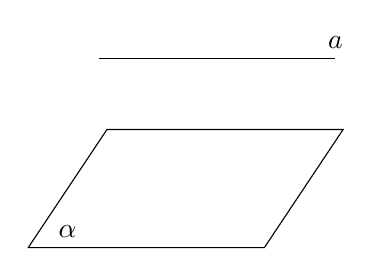
\begin{tikzpicture}
        \draw (0,0) -- (3,0) -- (4,1.5) -- (1,1.5) -- cycle;
        \draw (0.5,0) node [above] {$\alpha$};
        \draw (0.9,2.4) -- (3.9,2.4) node [above] {$a$}; 
    \end{tikzpicture}
    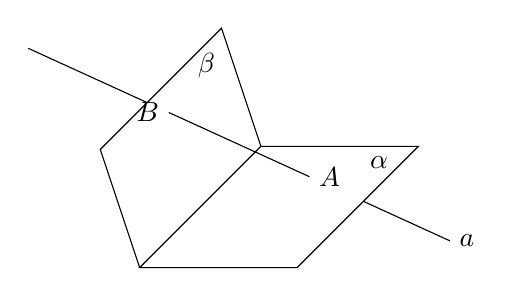
\begin{tikzpicture}
        \draw [name path = alpha] (0,0,0) -- (2,0,0) -- (2,0,-4)  -- (0,0,-4) -- cycle;
        \draw (1.5,0,-4) node [below] {$\alpha$};
        \draw [name path = beta] (0,0,0) -- (-0.5,1.5,0) -- (-0.5,1.5,-4)  -- (0,0,-4);
        \draw (-0.5,1.5,-3.5) node [below] {$\beta$};
        \draw (1,0,-3) node [right] {$A$} coordinate (A);
        \draw (-0.4,1.2,-2) node [left] {$B$} coordinate (B);
        \draw (A) -- (B);
        \path [name path = line1] ($(A)!-1!(B)$) coordinate (C) -- (A);
        \path [name path = line2] ($(B)!-1!(A)$) coordinate (D) -- (B);
        \path [name intersections = {of = line1 and alpha, by = S}];
        \draw (S) -- (C) node [right] {$a$};
        \path [name intersections = {of = line2 and beta, by = T}];
        \draw (T) -- (D);
    \end{tikzpicture}
\end{center}


关联目标:

暂未关联目标

答案: 暂无答案

解答或提示: 暂无解答与提示

使用记录:

暂无使用记录


出处: 二期课改练习册高三
\item { (009426)}判断下列各组对象能否组成集合. 若能组成集合, 指出是有限集还是无限集; 若不能组成集合, 请说明理由.\\
(1) 上海市现有各区的名称;\\
(2) 末位是$3$的自然数;\\
(3) 比较大的苹果.


关联目标:

暂未关联目标

答案: 暂无答案

解答或提示: 暂无解答与提示

使用记录:

暂无使用记录


出处: 新教材必修第一册课堂练习
\item { (009428)}用列举法表示下列集合:\\
(1) 能整除$10$的所有正整数组成的集合;\\
(2) 绝对值小于$4$的所有整数组成的集合.


关联目标:

暂未关联目标

答案: 暂无答案

解答或提示: 暂无解答与提示

使用记录:

暂无使用记录


出处: 新教材必修第一册课堂练习
\item { (009429)}用描述法表示下列集合:\\
(1) 全体偶数组成的集合;\\
(2) 平面直角坐标系中$x$轴上所有点组成的集合.


关联目标:

暂未关联目标

答案: 暂无答案

解答或提示: 暂无解答与提示

使用记录:

暂无使用记录


出处: 新教材必修第一册课堂练习
\item { (009430)}用区间表示下列集合:\\
(1) $\{x|-1<x\le 5\}$;\\
(2) 不等式$-2x>6$的所有解组成的集合.


关联目标:

暂未关联目标

答案: 暂无答案

解答或提示: 暂无解答与提示

使用记录:

暂无使用记录


出处: 新教材必修第一册课堂练习
\item { (009433)}写出所有满足$\{a\}\subset M\subset \{a, b, c, d\}$的集合$M$.


关联目标:

暂未关联目标

答案: 暂无答案

解答或提示: 暂无解答与提示

使用记录:

暂无使用记录


出处: 新教材必修第一册课堂练习
\item { (009435)}已知全集为$\mathbf{R}$, 集合$A=\{x|-2<x\le 1\}$. 求$A$.


关联目标:

暂未关联目标

答案: 暂无答案

解答或提示: 暂无解答与提示

使用记录:

暂无使用记录


出处: 新教材必修第一册课堂练习
\item { (009436)}已知集合$A=\{1, 2, 3, 4, 5\}$, $B=\{2, 4, 6, 8\}$, $C=\{3, 4, 5, 6\}$. 求:\\
(1) $(A\cap B)\cup C$, $(A\cup C)\cap (B\cup C)$;\\
(2) $(A\cup B)\cap C$, $(A\cap C)\cup (B\cap C)$.


关联目标:

暂未关联目标

答案: 暂无答案

解答或提示: 暂无解答与提示

使用记录:

暂无使用记录


出处: 新教材必修第一册课堂练习
\item { (009437)}举几个生活中的命题的例子, 并判断其真假.


关联目标:

暂未关联目标

答案: 暂无答案

解答或提示: 暂无解答与提示

使用记录:

暂无使用记录


出处: 新教材必修第一册课堂练习
\item { (009438)}判断下列命题的真假, 并说明理由:\\
(1) 所有偶数都不是素数;\\
(2) $\{1\}$是$\{0, 1, 2\}$的真子集;\\
(3) $0$是$\{0, 1, 2\}$的真子集;\\
(4) 如果集合$A$是集合$B$的子集, 那么$B$不是$A$的子集.


关联目标:

暂未关联目标

答案: 暂无答案

解答或提示: 暂无解答与提示

使用记录:

暂无使用记录


出处: 新教材必修第一册课堂练习
\item { (009444)}设$a$、$b$、$c$、$d$是实数, 判断下列命题的真假, 并说明理由:\\
(1) 若$a^2=b^2$, 则$a=b$;\\
(2) 若$a(c^2+1)=b(c^2+1)$, 则$a=b$;\\
(3) 若$ab=0$, 则$a=0$或$b=0$;\\
(4) 若$\dfrac ac=\dfrac bd$, 且$c+d\ne 0$, 则$\dfrac{a+b}{c+d}=\dfrac ac$.


关联目标:

暂未关联目标

答案: 暂无答案

解答或提示: 暂无解答与提示

使用记录:

暂无使用记录


出处: 新教材必修第一册课堂练习
\item { (009449)}设$a$、$b$、$c$、$d$为实数, 判断下列命题的真假, 并说明理由:\\
(1) 如果$a>b$, $c>d$, 那么$a+d>b+c$;\\
(2) 如果$ab>ac$, 那么$b>c$;\\
(3) 如果$a\ge b$且$a\le b$, 那么$a=b$;\\
(4) 如果$a>b$, $\dfrac 1c>\dfrac 1d$, 那么$ac>bd$;\\
(5) 如果$\dfrac ba>\dfrac dc$, 那么$bc>ad$.


关联目标:

暂未关联目标

答案: 暂无答案

解答或提示: 暂无解答与提示

使用记录:

暂无使用记录


出处: 新教材必修第一册课堂练习
\item { (009451)}设$a$、$b$、$c$是实数, 判断下列命题的真假, 并说明理由.\\
(1) 如果$ac^2>bc^2$, 那么$a>b$;\\
(2) 如果$ab>c$, 那么$a>\dfrac cb$;\\
(3) 如果$a>b\ge 0$, 那么$\sqrt a>\sqrt b$.


关联目标:

暂未关联目标

答案: 暂无答案

解答或提示: 暂无解答与提示

使用记录:

暂无使用记录


出处: 新教材必修第一册课堂练习
\item { (009539)}判断下列命题是否正确:\\
(1) 终边重合的两个角相等;\\
(2) 锐角是第一象限的角;\\
(3) 第二象限的角是钝角;\\
(4) 小于$90^\circ$的角都是锐角.


关联目标:

暂未关联目标

答案: 暂无答案

解答或提示: 暂无解答与提示

使用记录:

暂无使用记录


出处: 新教材必修第二册课堂练习
\item { (009540)}分别用集合的形式表示终边位于第三象限的所有角和终边位于$y$轴正半轴上的所有角.


关联目标:

暂未关联目标

答案: 暂无答案

解答或提示: 暂无解答与提示

使用记录:

暂无使用记录


出处: 新教材必修第二册课堂练习
\item { (009563)}分别求满足下列条件的角$x$的集合:\\
(1) $2\sin (x+\dfrac\pi 3)=1$, $x\in [0, 2\pi ]$;\\
(2) $\cos (2x+\dfrac \pi 4)=-\dfrac 12$;\\
(3) $\tan (3x+\dfrac \pi 4)=-1$.


关联目标:

暂未关联目标

答案: 暂无答案

解答或提示: 暂无解答与提示

使用记录:

暂无使用记录


出处: 新教材必修第二册课堂练习
\item { (009610)}写出满足$\tan \alpha=\sqrt 3$的所有$\alpha$的集合.


关联目标:

暂未关联目标

答案: 暂无答案

解答或提示: 暂无解答与提示

使用记录:

暂无使用记录


出处: 新教材必修第二册课堂练习
\item { (009647)}下列关于复数$z$和$\overline z$的命题是真命题还是假命题? 请给出结论并说明理由.\\
(1) $z+\overline z$一定是实数;\\
(2) $z-\overline z$一定是纯虚数;\\
(3) $若z-\overline z=0$, 则$z$是实数;\\
(4) 若$z+\overline z=0$, 则z是纯虚数.


关联目标:

暂未关联目标

答案: 暂无答案

解答或提示: 暂无解答与提示

使用记录:

暂无使用记录


出处: 新教材必修第二册课堂练习
\item { (009664)}如图, 用集合语言描述下列图形中的点、直线、平面之间的位置关系.
\begin{center}
(1) 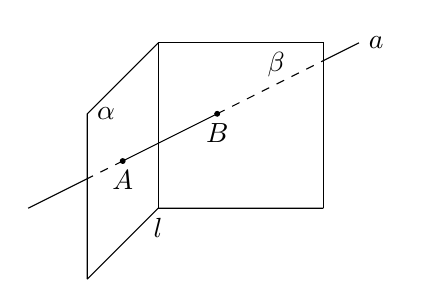
\begin{tikzpicture}[>=latex,scale = 1.5]
\draw (1,0.4) -- (1.6,1) -- (3,1);
\draw (1.6,1) -- (1.6,2.4);
\draw [name path = rightside] (3,1) -- (3,2.4) -- (1.6,2.4);
\draw [name path = leftside] (1,0.4) -- (1,1.8) -- (1.6,2.4);
\filldraw (1.3,1.4) circle (0.02) node [below] {$A$} coordinate (A) (2.1,1.8) circle (0.02) node [below] {$B$} coordinate (B);
\path [name path = leftline] ($(A)!-1!(B)$)  coordinate (S) -- (A);
\path [name path = rightline] ($(A)!2.5!(B)$) coordinate (T) -- (B);
\path [name intersections = {of = leftside and leftline, by = C}];
\path [name intersections = {of = rightside and rightline, by = D}];
\draw (D) -- (T) node [right] {$a$} (C) -- (S) (A) -- (B);
\draw [dashed] (A) -- (C) (B) -- (D);
\draw (1.6,1) node [below] {$l$};
\draw (1,1.8) node [right] {$\alpha$} (2.6,2.4) node [below] {$\beta$};
\end{tikzpicture}
(2) 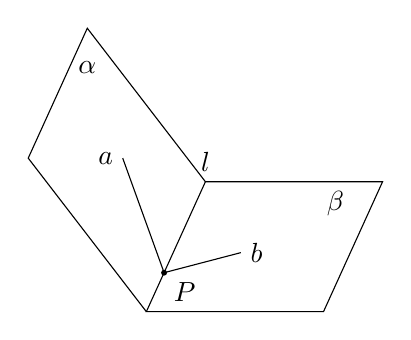
\begin{tikzpicture}[>=latex,scale = 1.5]
    \draw (1.2,0.4) coordinate (X) -- (2.7,0.4) -- (3.2,1.5) -- (1.7,1.5) coordinate (Y) -- cycle;
    \draw (X) -- (0.2,1.7) --++ (0.5,1.1)  -- (Y) node [above] {$l$};
    \draw (0.7,2.6) node [below] {$\alpha$} (2.8,1.5) node [below] {$\beta$};
    \filldraw ($(X)!0.3!(Y)$) circle (0.02) node [below right] {$P$} coordinate (T);
    \draw (T) -- (1,1.7) node [left] {$a$} (T) -- (2,0.9) node [right] {$b$};
    \end{tikzpicture}
\end{center}


关联目标:

暂未关联目标

答案: 暂无答案

解答或提示: 暂无解答与提示

使用记录:

暂无使用记录


出处: 新教材必修第三册课堂练习
\item { (009683)}判断下列命题的真假, 并说明理由:\\
(1) 若直线$a$上有无数个点不在平面$\alpha$上, 则$a\parallel \alpha$;\\
(2) 若直线$a$与平面$\alpha$上的一条直线平行, 则$a$与平面$\alpha$上的任意一条直线都平行;\\
(3) 若两条平行直线中的一条平行于一个平面, 则另一条直线也平行于这个平面;\\
(4) 设直线$a$在平面$\alpha$上, 直线$b$不在平面$\alpha$上, 并且$a\parallel b$, 则$b\parallel \alpha$.


关联目标:

暂未关联目标

答案: 暂无答案

解答或提示: 暂无解答与提示

使用记录:

暂无使用记录


出处: 新教材必修第三册课堂练习
\item { (009685)}判断下列命题的真假, 并说明理由:\\
(1) 若两直线$a$、$b$互相平行, 则$a$平行于经过$b$的任何平面;\\
(2) 若直线$a$与平面$\alpha$平行, 则$a$平行于$\alpha$内的任何直线;\\
(3) 若两直线$a$、$b$都与平面$\alpha$平行, 则$a\parallel b$;\\
(4) 若直线$a$平行于平面$\alpha$, 直线$b$在平面$\alpha$上, 则$a\parallel b$或者$a$与$b$为异面直线.


关联目标:

暂未关联目标

答案: 暂无答案

解答或提示: 暂无解答与提示

使用记录:

暂无使用记录


出处: 新教材必修第三册课堂练习
\item { (009697)}判断下列命题的真假, 并说明理由:\\
(1) 若一个平面内的两条直线均平行于另一个平面, 则这两个平面平行;
(2) 若一个平面内两条不平行的直线都平行于另一个平面, 则这两个平面平行;
(3) 若两个平面平行, 则其中一个平面中的任何直线都平行于另一个平面;
(4) 平行于同一个平面的两个平面平行;
(5) 若一个平面内的任何一条直线都平行于另一个平面, 则这两个平面平行.


关联目标:

暂未关联目标

答案: 暂无答案

解答或提示: 暂无解答与提示

使用记录:

暂无使用记录


出处: 新教材必修第三册课堂练习
\item { (009700)}已知平面$\alpha\perp$平面$\beta$, 判断下列命题是否正确, 并说明理由:\\ 
(1) 平面$\alpha$上的任意一条直线都垂直于平面$\beta$上的任意一条直线;\\
(2) 平面$\alpha$上的任意一条直线都垂直于平面$\beta$上的无数条直线;\\
(3) 平面$\alpha$上的任意一条直线都垂直于平面$\beta$;\\
(4) 过平面$\alpha$上任意一点作平面$\alpha$与$\beta$交线的垂线$l$, 则$l\perp \beta$.


关联目标:

暂未关联目标

答案: 暂无答案

解答或提示: 暂无解答与提示

使用记录:

暂无使用记录


出处: 新教材必修第三册课堂练习
\item { (009860)}下列命题是否为真命题? 如果是, 请说明理由; 如果不是, 请举出反例.\\
(1) 设$A$、$B$、$C$、$D$是空间中的四个不同的点, 直线$AB$与$CD$是异面直线, 则向量$\overrightarrow{AB}$与$\overrightarrow{CD}$不共面;\\
(2) 如果$\overrightarrow a$、$\overrightarrow b$是平面$\alpha$上的互不平行的向量, 点$C$、$D$不在平面$\alpha$上, 那么向量$\overrightarrow{CD}$与向量$\overrightarrow a$、$\overrightarrow b$不共面;\\
(3) 如果$\overrightarrow a$、$\overrightarrow b$是平面$\alpha$上的互不平行的向量, 点$C$在平面$\alpha$上, 点$D$不在平面$\alpha$上, 那么向量$\overrightarrow{CD}$与向量$\overrightarrow a$、$\overrightarrow b$不共面.


关联目标:

暂未关联目标

答案: 暂无答案

解答或提示: 暂无解答与提示

使用记录:

暂无使用记录


出处: 新教材选择性必修第一册课堂练习
\item { (009995)}设定义在$[0,+\infty)$上的函数$f(x)$的值域为$A_f$. 若对任意满足$f(x)=f(\dfrac 1{x+1})$的函数$f(x)$, 集合$\{y|y=f(x), \ x\in [0,a]\}$总可以取得$A_f$中的所有值, 则实数$a$的取值范围为\blank{50}.


关联目标:

暂未关联目标

答案: 暂无答案

解答或提示: 暂无解答与提示

使用记录:

暂无使用记录


出处: 上海2022年秋季高考试题12
\item { (009996)}若集合$A=[-1,2)$, $B=\mathbf{Z}$, 则$A\cap B=$\bracket{20}.
\fourch{$\{-2,-1,0,1\}$}{$\{-1,0,1\}$}{$\{-1,0\}$}{$\{-1\}$}


关联目标:

暂未关联目标

答案: 暂无答案

解答或提示: 暂无解答与提示

使用记录:

暂无使用记录


出处: 上海2022年秋季高考试题13
\item { (009999)}设集合$\Omega = \{(x,y)|(x-k)^2+(y-k^2)^2=4|k|, \ k\in \mathbf{Z}\}$. 关于命题:
\textcircled{1} ``存在直线$l$, 使得集合$\Omega$中不存在点在$l$上, 而存在点在$l$两侧''; \textcircled{2} ``存在直线$l$, 使得集合$\Omega$中存在无数点在$l$上''的真假判断, 正确的是\bracket{20}.
\twoch{\textcircled{1}和\textcircled{2}都是真命题}{\textcircled{1}是真命题, \textcircled{2}是假命题}{\textcircled{1}是假命题, \textcircled{2}是真命题}{\textcircled{1}和\textcircled{2}都是假命题}


关联目标:

暂未关联目标

答案: 暂无答案

解答或提示: 暂无解答与提示

使用记录:

暂无使用记录


出处: 上海2022年秋季高考试题16
\item { (010004)}数列$\{a_n\}$中, $a_1=1$, $a_2=3$, 且对任意$n$($n\ge 2$), 都存在$i$($1\le i\le n-1$), 使得$a_{n+1}=2a_n-a_i$.\\
(1) 求$a_4$的所有可能值;\\
(2) 命题$p$: 若$a_1,a_2,a_3,\cdots,a_8$成等差数列, 则$a_9<30$成立. 证明命题$p$为真, 写出命题$p$的逆命题$q$; 若命题$q$为真, 则证明, 若命题$q$为假, 请举出反例;\\
(3) 对任意正整数$m$, $a_{2m}=3^m$, 求$\{a_n\}$的通项公式.


关联目标:

暂未关联目标

答案: 暂无答案

解答或提示: 暂无解答与提示

使用记录:

暂无使用记录


出处: 上海2022年秋季高考试题21
\item { (010016)}设随机变量$X$的取值在集合$\{0,1,2\}$中.\\
(1) 若$P(X=1)=\dfrac 12$, 求期望$E[X]$的最大可能值$M$与$E[X]$的最小可能值$m$之差;\\
(2) 猜测方差$D[X]$的最大可能值, 并证明你的猜测.


关联目标:

暂未关联目标

答案: $1$, $1$.

解答或提示: (1) $M=\dfrac 32$, $m=\dfrac 12$.\\
(2) 设$P(X=0)=p$, $P(X=2)=q$, 则$P(X=1)=1-p-q$, 其中$p\ge 0$, $q\ge 0$, $p+q\le 1$.\\
$E[X]=1\cdot (1-p-q)+2q=1-p+q$, $E[X^2]=1(1-p-q)+4q=1-p+3q$. 故$D[X]=1-p+3q-(1-p+q)^2=p+q-(p-q)^2\le 1+0=1$.\\
而当$p=q=\dfrac 12$时, $D[X]$能取到$1$, 故$D[X]$的最大可能值为$1$.

使用记录:

20220802	2023届高三2班	\fcolorbox[rgb]{0,0,0}{1.000,0.332,0}{0.834}	\fcolorbox[rgb]{0,0,0}{0.076,1.000,0}{0.038}

20220802	2023届高三11班	\fcolorbox[rgb]{0,0,0}{0.666,1.000,0}{0.333}	\fcolorbox[rgb]{0,0,0}{0.084,1.000,0}{0.042}

20220802	2023届高三10班	\fcolorbox[rgb]{0,0,0}{1.000,0.700,0}{0.650}	\fcolorbox[rgb]{0,0,0}{0.026,1.000,0}{0.013}

20220802	2023届高三5班	\fcolorbox[rgb]{0,0,0}{1.000,0.500,0}{0.750}	\fcolorbox[rgb]{0,0,0}{0.074,1.000,0}{0.037}

20220802	2023届高三8班	\fcolorbox[rgb]{0,0,0}{1.000,0.484,0}{0.758}	\fcolorbox[rgb]{0,0,0}{0.182,1.000,0}{0.091}

20220802	2023届高三7班	\fcolorbox[rgb]{0,0,0}{1.000,0.858,0}{0.571}	\fcolorbox[rgb]{0,0,0}{0.094,1.000,0}{0.047}

20220802	2023届高三4班	\fcolorbox[rgb]{0,0,0}{1.000,0.438,0}{0.781}	\fcolorbox[rgb]{0,0,0}{0.026,1.000,0}{0.013}

20220802	2023届高三9班	\fcolorbox[rgb]{0,0,0}{1.000,0.288,0}{0.856}	\fcolorbox[rgb]{0,0,0}{0.026,1.000,0}{0.013}

20220802	2023届高三12班	\fcolorbox[rgb]{0,0,0}{1.000,0.462,0}{0.769}	\fcolorbox[rgb]{0,0,0}{0.016,1.000,0}{0.008}

20220802	2023届高三3班	\fcolorbox[rgb]{0,0,0}{1.000,0.064,0}{0.968}	\fcolorbox[rgb]{0,0,0}{0.064,1.000,0}{0.032}

20220802	2023届高三1班	\fcolorbox[rgb]{0,0,0}{1.000,0.020,0}{0.990}	\fcolorbox[rgb]{0,0,0}{0.540,1.000,0}{0.270}

20220802	2023届高三6班	\fcolorbox[rgb]{0,0,0}{1.000,0.230,0}{0.885}	\fcolorbox[rgb]{0,0,0}{0.260,1.000,0}{0.130}


出处: 2023届高三前暑假概率初步续单元测验
\item { (010017)}用列举法表示下列集合:\\
(1) $10$以内的所有素数组成的集合;\\
(2) $\{y|y=x-1,\  0\le x\le 3,\ x\in \mathbf{Z}\}$.


关联目标:

暂未关联目标

答案: 暂无答案

解答或提示: 暂无解答与提示

使用记录:

暂无使用记录


出处: 新教材必修第一册习题
\item { (010018)}用描述法表示下列集合:\\
(1) 被$3$除余$1$的所有自然数组成的集合;\\
(2) 比$1$大又比$10$小的所有实数组成的集合;\\
(3) 平面直角坐标系中坐标轴上所有点组成的集合.


关联目标:

暂未关联目标

答案: 暂无答案

解答或提示: 暂无解答与提示

使用记录:

暂无使用记录


出处: 新教材必修第一册习题
\item { (010019)}集合$\{(x, y)|xy>0, \ x,y\text{为实数}\}$是指\bracket{20}.
\twoch{第一象限内的所有点组成的集合}{第三象限内的所有点组成的集合}{第一象限和第三象限内的所有点组成的集合}{不在第二象限也不在第四象限内的所有点组成的集合}


关联目标:

暂未关联目标

答案: 暂无答案

解答或提示: 暂无解答与提示

使用记录:

暂无使用记录


出处: 新教材必修第一册习题
\item { (010020)}用符号``$\subset$''``$=$''或``$\supset$''连接集合$A$与$B$:\\
(1) $A=\{x|x^2-2x+1=0\}$, $B=\{x|x^2-1=0\}$;\\
(2) $A=\{1, 2, 4, 8\}$, $B=\{x|x$是$8$的正约数$\}$.


关联目标:

暂未关联目标

答案: 暂无答案

解答或提示: 暂无解答与提示

使用记录:

暂无使用记录


出处: 新教材必修第一册习题
\item { (010021)}已知集合$A=\{1\}$, $B=\{x|x^2-3x+a=0\}$. 是否存在实数$a$, 使得$A\subset B$?  若存在, 求$a$的值; 若不存在, 说明理由.


关联目标:

暂未关联目标

答案: 暂无答案

解答或提示: 暂无解答与提示

使用记录:

暂无使用记录


出处: 新教材必修第一册习题
\item { (010022)}已知集合$A=\{x, y\}$, $B=\{2x, 2x^2\}$, 且$A=B$. 求集合$A$.


关联目标:

暂未关联目标

答案: 暂无答案

解答或提示: 暂无解答与提示

使用记录:

暂无使用记录


出处: 新教材必修第一册习题
\item { (010023)}已知集合$A=\{x|x\le 7\}$, $B=\{x|x<2\}$, $C=\{x|x>5\}$. 求: $A\cap B$, $A\cap C$, $A\cap (B\cap C)$.


关联目标:

暂未关联目标

答案: 暂无答案

解答或提示: 暂无解答与提示

使用记录:

暂无使用记录


出处: 新教材必修第一册习题
\item { (010024)}已知集合$A=\{(x, y)|y=-x+1\}$, $B=\{(x, y)|y=x^2-1\}$. 求$A\cap B$.


关联目标:

暂未关联目标

答案: 暂无答案

解答或提示: 暂无解答与提示

使用记录:

暂无使用记录


出处: 新教材必修第一册习题
\item { (010025)}已知全集$U=\mathbf{R}$, 集合$A=\{x|4-x>2x+1\}$. 求$\overline A$.


关联目标:

暂未关联目标

答案: 暂无答案

解答或提示: 暂无解答与提示

使用记录:

暂无使用记录


出处: 新教材必修第一册习题
\item { (010026)}已知集合$A=\{2, (a+1)^2, a^2+3a+3\}$, 且$1\in A$. 求实数$a$的值.


关联目标:

暂未关联目标

答案: 暂无答案

解答或提示: 暂无解答与提示

使用记录:

暂无使用记录


出处: 新教材必修第一册习题
\item { (010027)}已知集合$A=\{x|x=2n+1,\ n\in \mathbf{Z}\}$, $B=\{x|x=4n-1,\ n\in \mathbf{Z}\}$. 判断集合$A$与$B$的包含关系, 并证明你的结论.


关联目标:

暂未关联目标

答案: 暂无答案

解答或提示: 暂无解答与提示

使用记录:

暂无使用记录


出处: 新教材必修第一册习题
\item { (010028)}设$a$是实数, 集合$M=\{x|x^2+x-6=0\}$, $N=\{y|ay+2=0\}$. 是否存在$a$, 使得$N\subset M$? 若存在, 求这些$a$的值; 若不存在, 说明理由.


关联目标:

暂未关联目标

答案: 暂无答案

解答或提示: 暂无解答与提示

使用记录:

暂无使用记录


出处: 新教材必修第一册习题
\item { (010029)}已知集合$A=\{1, 4, x\}$, $B=\{1, x^2\}$, 且$A\cup B=A$. 求$x$的值及集合$A$、$B$.


关联目标:

暂未关联目标

答案: 暂无答案

解答或提示: 暂无解答与提示

使用记录:

暂无使用记录


出处: 新教材必修第一册习题
\item { (010030)}判断下列语句是否为命题:\\
(1) 有的正方形是三角形;\\
(2) 任意一个三角形的内角和都为$180^\circ$;\\
(3) $1$是自然数吗?\\
(4) $3>\pi$;\\
(5) $2\in (0, 5)$, 且$2\in \mathbf{Z}$.


关联目标:

暂未关联目标

答案: 暂无答案

解答或提示: 暂无解答与提示

使用记录:

暂无使用记录


出处: 新教材必修第一册习题
\item { (010031)}判断下列命题的真假, 并说明理由:\\
(1) 如果$a$、$b$都是奇数, 那么$a+b$是偶数;\\
(2) 一组对边平行且两对角线等长的四边形是平行四边形;\\
(3) 如果$A\cap B=A$, 那么$A\cup B=B$.


关联目标:

暂未关联目标

答案: 暂无答案

解答或提示: 暂无解答与提示

使用记录:

暂无使用记录


出处: 新教材必修第一册习题
\item { (010033)}下列各组中, $\alpha$是$\beta$的什么条件?\\
(1) $\alpha$: 四边形$ABCD$的四条边等长, $\beta$: 四边形$ABCD$是正方形;\\
(2) $\alpha$: $\triangle ABC$与$\triangle DEF$全等, $\beta$: $\triangle ABC$与$\triangle DEF$的周长相等;\\
(3) $\alpha$: $x$是$2$的倍数, $\beta$: $x$是$6$的倍数;\\
(4) $\alpha$: 集合$A\subseteq B$, $B\subseteq C$, $C\subseteq A$, $\beta$: 集合$A=B=C$;\\
(5) $\alpha$: $A\cap B=A\cap C$, $\beta$: $B=C$.


关联目标:

暂未关联目标

答案: 暂无答案

解答或提示: 暂无解答与提示

使用记录:

暂无使用记录


出处: 新教材必修第一册习题
\item { (010036)}判断下列命题的真假, 并说明理由:\\
(1) 若$A\cap B=\varnothing$, $C\subset B$, 则$A\cap C=\varnothing$;\\
(2) 若$a$、$b\in \mathbf{R}$, 则关于$x$的方程$(a+1)x+b=0$的解为$x=- \dfrac b{a+1}$.


关联目标:

暂未关联目标

答案: 暂无答案

解答或提示: 暂无解答与提示

使用记录:

暂无使用记录


出处: 新教材必修第一册习题
\item { (010046)}设$a$、$b$、$c$、$d$为实数, 判断下列命题的真假:\\
(1) 若$a>b\ge 0$, 则$a^2>b^2$;\\
(2) 若$\sqrt a>\sqrt b$, 则$a>b$;\\
(3) 若$a>b>0, c>d>0$, 则$ac>bd$;\\
(4) 若$\dfrac ba>0$, 则$ab>0$;\\
(5) 若$a>b>0$, 则$a^2>ab>b^2$;\\
(6) 若$\sqrt a>b$, 则$a>b^2$.


关联目标:

暂未关联目标

答案: 暂无答案

解答或提示: 暂无解答与提示

使用记录:

暂无使用记录


出处: 新教材必修第一册习题
\item { (010065)}原有酒精溶液$a$(单位: $\text{g}$), 其中含有酒精$b$(单位: $\text{g}$), 其酒精浓度为$\dfrac ba$. 为增加酒精浓度, 在原溶液中加入酒精$x$(单位: $\text{g}$), 新溶液的浓度变为$\dfrac{b+x}{a+x}$. 根据这一事实, 可提炼出如下关于不等式的命题:若$a>b>0$, $x>0$, 则$\dfrac ba<\dfrac{b+x}{a+x}<1$. 试加以证明.


关联目标:

暂未关联目标

答案: 暂无答案

解答或提示: 暂无解答与提示

使用记录:

暂无使用记录


出处: 新教材必修第一册习题
\item { (010069)}设全集为$\mathbf{R}$, 集合$A=\{x|x^2-2x-3\ge 0\}$
, $B=\{x|x^2+x-2<0\}$. 求:\\
(1) $A\cup B$;\\
(2) $A\cap B$;\\
(3) $\overline{A\cap B}$;\\
(4) $\overline A\cup \overline B$.


关联目标:

暂未关联目标

答案: 暂无答案

解答或提示: 暂无解答与提示

使用记录:

暂无使用记录


出处: 新教材必修第一册习题
\item { (010089)}如果实数$a$、$b$同号, 那么下列命题中正确的是\bracket{20}.
\fourch{$a^2+b^2>2ab$}{$a+b\ge 2\sqrt {ab}$}{$\dfrac 1a+\dfrac 1b> \dfrac 2{\sqrt {ab}}$}{$\dfrac ba+\dfrac ab\ge 2$}


关联目标:

暂未关联目标

答案: 暂无答案

解答或提示: 暂无解答与提示

使用记录:

暂无使用记录


出处: 新教材必修第一册习题
\item { (010137)}下列命题中, 正确的是\bracket{20}.
\onech{当$n=0$时, 函数$y=x^n$的图像是一条直线}{幂函数$y=x^n$的图像都经过$(0, 0)$和$(1, 1)$两个点}{若幂函数$y=x^n$的图像关于原点成中心对称, 则$y=x^n$在区间$(-\infty, 0)$上是严格增函数}{幂函数的图像不可能在第四象限}


关联目标:

暂未关联目标

答案: 暂无答案

解答或提示: 暂无解答与提示

使用记录:

暂无使用记录


出处: 新教材必修第一册习题
\item { (010221)}写出与下列各角的终边重合的所有角组成的集合$S$, 并写出$S$中适合不等式$-360^\circ \le \alpha<720^\circ$的元素$\alpha$:\\
(1) $60^\circ$;\\
(2) $-21^\circ$.


关联目标:

暂未关联目标

答案: 暂无答案

解答或提示: 暂无解答与提示

使用记录:

暂无使用记录


出处: 新教材必修第二册习题
\item { (010224)}写出终边在直线$y=x$上的所有角组成的集合. (分别用角度制和弧度制来表示)


关联目标:

暂未关联目标

答案: 暂无答案

解答或提示: 暂无解答与提示

使用记录:

暂无使用记录


出处: 新教材必修第二册习题
\item { (010276)}求下列函数的最大值和最小值, 并指出使其取得最大值和最小值时的所有$x$值的集合:\\
(1) $y=2-3\sin x$, $x\in \mathbf{R}$;\\
(2) $y=-\sin^2x+2\sin x+2$, $x\in \mathbf{R}$;\\
(3) $y=2\sin x-5$, $x\in [-\dfrac \pi 3, \dfrac{5\pi} 6]$;\\
(4) $y=\cos^2x-\sin x$, $x\in \mathbf{R}$.


关联目标:

暂未关联目标

答案: 暂无答案

解答或提示: 暂无解答与提示

使用记录:

暂无使用记录


出处: 新教材必修第二册习题
\item { (010291)}求下列函数的最大值和最小值, 并指出使其取得最大值和最小值时$x$的集合:\\
(1) $y=3^{\cos 2x}$, $x\in \mathbf{R}$;\\
(2) $y=\cos x-\sin^2x$, $x\in \mathbf{R}$.


关联目标:

暂未关联目标

答案: 暂无答案

解答或提示: 暂无解答与提示

使用记录:

暂无使用记录


出处: 新教材必修第二册习题
\item { (010315)}判断下列命题的真假, 并说明理由:\\
(1) 长度相等的向量均为相等向量;\\
(2) 给定向量$\overrightarrow a$、$\overrightarrow b$、$\overrightarrow c$, 若$\overrightarrow a=\overrightarrow b$, $\overrightarrow b=\overrightarrow c$, 则$\overrightarrow a=\overrightarrow c$;\\
(3) 若$ABCD$为平行四边形, 则必有$\overrightarrow{AB}=\overrightarrow{CD}$;\\
(4) 若平面上四点$A$、$B$、$C$、$D$使$\overrightarrow{AB}=\overrightarrow{CD}$, 则$AB\parallel CD$.


关联目标:

暂未关联目标

答案: 暂无答案

解答或提示: 暂无解答与提示

使用记录:

暂无使用记录


出处: 新教材必修第二册习题
\item { (010329)}判断下列命题的真假, 并说明理由:\\
(1) 若存在一个$\lambda \in \mathbf{R}$使$\lambda \overrightarrow a=\lambda \overrightarrow b$, 则$\overrightarrow a=\overrightarrow b$;\\
(2) 对于任意给定的实数$\lambda$和向量$\overrightarrow a$、$\overrightarrow b$, 均有$\lambda (\overrightarrow a-\overrightarrow b)=\lambda \overrightarrow a-\lambda \overrightarrow b$;\\
(3) 对于任意给定的实数$\lambda$、$\mu$和向量$\overrightarrow a$, 均有$(\lambda -\mu)\overrightarrow a=\lambda \overrightarrow a-\mu\overrightarrow a$.


关联目标:

暂未关联目标

答案: 暂无答案

解答或提示: 暂无解答与提示

使用记录:

暂无使用记录


出处: 新教材必修第二册习题
\item { (010413)}证明: 集合$M=\{z|z=\cos \theta +\mathrm{i}\sin \theta,\ \theta \in \mathbf{R}\}$中的所有复数在复平面上所对应的点在同一个圆上.


关联目标:

暂未关联目标

答案: 暂无答案

解答或提示: 暂无解答与提示

使用记录:

暂无使用记录


出处: 新教材必修第二册习题
\item { (010430)}用集合符号表述下列语句, 并将语句所描述的图形画在图中:\\
\begin{center}
\begin{tikzpicture}[>=latex]
\draw (0,0) -- (3,0) --++ (1,1.5) ++ (-0.5,0) node [below] {$\beta$} ++ (0.5,0) --++ (-3,0) -- (0,0);
\draw (0,0) --++ (-1.5,2) --++ (1,1.5) ++ (0.1,-0.2) node [below] {$\alpha$} ++ (-0.1,0.2) --++ (1.5,-2);
\end{tikzpicture}
\end{center}
(1) 点$A$在平面$\alpha$上:\blank{50};\\
(2) 平面$\alpha$经过直线$AC$:\blank{50};\\
(3) 点$B$不在平面$\beta$上:\blank{50};\\
(4) 直线$BC$平行于平面$\beta$:\blank{50}.


关联目标:

暂未关联目标

答案: 暂无答案

解答或提示: 暂无解答与提示

使用记录:

暂无使用记录


出处: 新教材必修第三册习题
\item { (010432)}判断下列命题的真假:\\
(1) 若空间四点共面, 则其中必有三点共线;\\
(2) 若空间四点中有三点共线, 则此四点必共面;\\
(3) 若空间四点中任何三点不共线, 则此四点不共面;\\
(4) 若空间四点不共面, 则其中任意三点不共线.


关联目标:

暂未关联目标

答案: 暂无答案

解答或提示: 暂无解答与提示

使用记录:

暂无使用记录


出处: 新教材必修第三册习题
\item { (010471)}判断下列命题的真假, 并说明理由:\\
(1) 平行于同一条直线的两个平面平行;\\
(2) 若两个平面分别经过两条平行直线, 则这两个平面平行;\\
(3) 分别在两个平行平面上的两条直线平行;\\
(4) 与两条异面直线都平行的两个平面平行.


关联目标:

暂未关联目标

答案: 暂无答案

解答或提示: 暂无解答与提示

使用记录:

暂无使用记录


出处: 新教材必修第三册习题
\item { (010479)}判断下列命题的真假, 并说明理由:\\
(1) 若平面$\alpha\perp$平面$\beta$, 平面$\beta\perp$平面$\gamma$, 则平面$\alpha\perp$平面$\gamma$;\\
(2) 若平面$\alpha\parallel$平面$\alpha_1$, 平面$\beta\parallel$平面$\beta_1$, 平面$\alpha\perp$平面$\beta$, 则平面$\alpha_1\perp$平面$\beta_1$.


关联目标:

暂未关联目标

答案: 暂无答案

解答或提示: 暂无解答与提示

使用记录:

暂无使用记录


出处: 新教材必修第三册习题
\item { (010538)}下列哪些是不确定的事件?\\
(1) 学生甲明天竞选班长成功;\\
(2) 两支足球队明天比赛, 主场队取胜;\\
(3) 若集合$A$、$B$、$C$满足$A\subseteq B\subseteq C$, 则$A\subseteq C$.


关联目标:

暂未关联目标

答案: 暂无答案

解答或提示: 暂无解答与提示

使用记录:

暂无使用记录


出处: 新教材必修第三册习题
\item { (010543)}在分别写有数字$0$、$1$、$2$、$3$、$4$、$5$、$6$、$7$、$8$、$9$的$10$张一样的卡片中随机抽取$1$张. 设事件$A$: 出现奇数, 事件$B$: 出现偶数, 事件$C$: 大于$4$. 写出下列事件对应的集合:\\
(1) $A$、$C$同时发生;\\
(2) $B$、$C$至少有一个发生;\\
(3) $A$、$B$同时发生.


关联目标:

暂未关联目标

答案: 暂无答案

解答或提示: 暂无解答与提示

使用记录:

暂无使用记录


出处: 新教材必修第三册习题
\item { (010634)}已知集合$A=\{(x, y)|2x-(a+1)y-1=0\}$, $B=\{(x, y)|ax-y+1=0\}$, 且$A\cap B=\varnothing$. 求实数$a$的值.


关联目标:

暂未关联目标

答案: 暂无答案

解答或提示: 暂无解答与提示

使用记录:

暂无使用记录


出处: 新教材选择性必修第一册习题
\item { (010719)}在平面上有如下命题: ``若$O$为直线$AB$外的一点, 则点$P$在直线$AB$上的充要条件是: 存在实数$\lambda$、$\mu$, 满足$\overrightarrow{OP}=\lambda \overrightarrow{OA}+\mu \overrightarrow{OB}$, 且$\lambda +\mu=1$.'' 类比此


关联目标:

暂未关联目标

答案: 暂无答案

解答或提示: 暂无解答与提示

使用记录:

暂无使用记录


出处: 新教材选择性必修第一册习题
\item { (010834)}设集合$A=\{(x, y)|x\in \mathbf{Z}, \  y\in \mathbf{Z}, \  \text{且}|x|\le 6, \ |y|\le 7\}$, 则集合$A$中有多少个元素?


关联目标:

暂未关联目标

答案: 暂无答案

解答或提示: 暂无解答与提示

使用记录:

暂无使用记录


出处: 新教材选择性必修第二册习题
\item { (010843)}在方程$ax+by=0$中, 设系数$a$、$b$是集合$\{0, 1, 2, 3, 5, 7\}$中两个不同的元素. 求这些方程所表示的不同直线的条数.


关联目标:

暂未关联目标

答案: 暂无答案

解答或提示: 暂无解答与提示

使用记录:

暂无使用记录


出处: 新教材选择性必修第二册习题
\item { (020001)}判断下列各组对象能否组成集合, 若能组成集合, 指出是有限集还是无限集.\\
(1) 上海市控江中学$2022$年入学的全体高一年级新生;\\
(2) 中国现有各省的名称;\\
(3) 太阳、$2$、上海市;\\
(4) 大于$10$且小于$15$的有理数;\\
(5) 末位是$3$的自然数;\\
(6) 影响力比较大的中国数学家;\\
(7) 方程$x^2+x+3=0$的所有实数解;\\ 
(8) 函数$y=\dfrac 1x$图像上所有的点;\\ 
(9) 在平面直角坐标系中, 到定点$(0, 0)$的距离等于$1$的所有点;\\
(10) 不等式$3x-10<0$的所有正整数解;\\
(11) 所有的平面四边形.


关联目标:

暂未关联目标

答案: 暂无答案

解答或提示: 暂无解答与提示

使用记录:

暂无使用记录


出处: 2025届高一校本作业必修第一章
\item { (020003)}对于一个确定的实数$x$, 由$x$, $-x$, $|x|$, $-\sqrt{x^2}$中的一个值或几个值组成的所有集合中, 元素的个数最多有多少个?


关联目标:

暂未关联目标

答案: 暂无答案

解答或提示: 暂无解答与提示

使用记录:

暂无使用记录


出处: 2025届高一校本作业必修第一章
\item { (020004)}已知关于$x$的方程$\sqrt {x^2+4x+a}=x+2$, 若以该方程的所有解为元素组成的集合是无限集, 求实数$a$满足的条件.


关联目标:

暂未关联目标

答案: 暂无答案

解答或提示: 暂无解答与提示

使用记录:

暂无使用记录


出处: 2025届高一校本作业必修第一章
\item { (020005)}用列举法表示下列集合:\\
(1) $12$以内的素数组成的集合;\\
(2) 绝对值小于$3$的所有整数的集合;\\
(3) $\{x|\dfrac 6{3-x}\in\mathbf{N}, \ x\in\mathbf{Z}\}$;\\
(4) $\{y|y=x^2-1 , \ |x| \le 2, \ x\in\mathbf{Z}\}$;\\
(5) $\{( x,y)|y=x^2-1,\ |x|\le 2, \ x\in\mathbf{Z}\}$;\\
(6) $\{( x,y)|x +y=5, \ x\in\mathbf{N}, \ y\in\mathbf{N}\}$.


关联目标:

暂未关联目标

答案: 暂无答案

解答或提示: 暂无解答与提示

使用记录:

暂无使用记录


出处: 2025届高一校本作业必修第一章
\item { (020006)}用描述法表示下列集合:\\
(1) 所有奇数组成的集合;\\
(2) 被$3$除余数等于$2$的正整数的集合;\\
(3) 不小于$10$的实数组成的集合;\\
(4) 绝对值大于$4$的所有整数组成的集合;\\
(5) 平面直角坐标系内$y$轴上的点的坐标组成的集合;\\
(6) 在直线$y=2x+1$上所有的点的坐标组成的集合.


关联目标:

暂未关联目标

答案: 暂无答案

解答或提示: 暂无解答与提示

使用记录:

暂无使用记录


出处: 2025届高一校本作业必修第一章
\item { (020007)}用区间表示下列集合:\\
(1) $\{x|-2<x<7\}$;\\
(2) $\{x|-2\le\ x\le7\}$;\\
(3) $\{x|-2\le\ x<7\}$;\\
(4) 不等式$2x<5$的解集;\\
(5) 不等式$-x<5$的解集; \\
(6) 非负实数集.


关联目标:

暂未关联目标

答案: 暂无答案

解答或提示: 暂无解答与提示

使用记录:

暂无使用记录


出处: 2025届高一校本作业必修第一章
\item { (020008)}用适当的方法表示下列集合:\\
(1) 能被$10$整除的所有正整数组成的集合;\\
(2) 能整除$10$的所有正整数组成的集合;\\
(3) 方程$x^2+2=0$的实数解组成的集合;\\
(4) 方程组$\begin{cases}2x+y=0, \\ x-y+3=0\end{cases}$的所有解组成的集合;\\
(5) 两直线$y=2x+1$和$y=x-2$的交点组成的集合.


关联目标:

暂未关联目标

答案: 暂无答案

解答或提示: 暂无解答与提示

使用记录:

暂无使用记录


出处: 2025届高一校本作业必修第一章
\item { (020010)}集合$\{(x, y)|xy\ge 0,\  x\in\mathbf{R},\  y\in\mathbf{R}\}$是指\bracket{20}.
\twoch{第一象限内的所有点}{第三象限内的所有点}{第一象限和第三象限内的所有点}{不在第二象限、第四象限内的所有点}


关联目标:

暂未关联目标

答案: 暂无答案

解答或提示: 暂无解答与提示

使用记录:

暂无使用记录


出处: 2025届高一校本作业必修第一章
\item { (020011)}若集合$M=\{0,2,3,7\}$, $P=\{x|x=ab,\ a,b\in M, \ a\ne b\}$. 用列举法写出集合$P$.


关联目标:

暂未关联目标

答案: 暂无答案

解答或提示: 暂无解答与提示

使用记录:

暂无使用记录


出处: 2025届高一校本作业必修第一章
\item { (020012)}已知集合$A={2, a^2, a}$, 且$1\in A$, 求实数$a$的值.


关联目标:

暂未关联目标

答案: 暂无答案

解答或提示: 暂无解答与提示

使用记录:

暂无使用记录


出处: 2025届高一校本作业必修第一章
\item { (020013)}设集合$M=\{a|a=x^2-y^2, \ x,y\in\mathbf{Z}\}$, 下列数中不属于$M$的为\bracket{20}.
\fourch{$3$}{$6$}{$9$}{$12$}


关联目标:

暂未关联目标

答案: 暂无答案

解答或提示: 暂无解答与提示

使用记录:

暂无使用记录


出处: 2025届高一校本作业必修第一章
\item { (020014)}已知集合$A=\{x|x=a+\sqrt 2b,\ a,b\in \mathbf{Z}\}$, 若$x_1,x_2\in A$, 证明: $x_1x_2\in A$.


关联目标:

暂未关联目标

答案: 暂无答案

解答或提示: 暂无解答与提示

使用记录:

暂无使用记录


出处: 2025届高一校本作业必修第一章
\item { (020015)}已知集合$A=\{x|(k+1)x^2+x-k=0\}$中只有一个元素, 求实数$k$的值.


关联目标:

暂未关联目标

答案: 暂无答案

解答或提示: 暂无解答与提示

使用记录:

暂无使用记录


出处: 2025届高一校本作业必修第一章
\item { (020017)}集合$\{1,2,3\}$的子集共有\blank{50}个.


关联目标:

暂未关联目标

答案: 暂无答案

解答或提示: 暂无解答与提示

使用记录:

暂无使用记录


出处: 2025届高一校本作业必修第一章
\item { (020018)}已知集合$A=\{1,2\}$, 集合$B=\{1,2,3,4,5\}$. 若集合$M$满足$A\subset M$且$M\subseteq B$, 则这样的集合$M$有\blank{50}个.


关联目标:

暂未关联目标

答案: 暂无答案

解答或提示: 暂无解答与提示

使用记录:

暂无使用记录


出处: 2025届高一校本作业必修第一章
\item { (020019)}满足$\{a, b\}\subset M \subset\{a, b, c, d, e\}$的集合$M$有\blank{50}个.


关联目标:

暂未关联目标

答案: 暂无答案

解答或提示: 暂无解答与提示

使用记录:

暂无使用记录


出处: 2025届高一校本作业必修第一章
\item { (020021)}下列各选项中, $M$与$P$表示同一个集合的有\blank{50}.\\
\textcircled{1} $M=\{(1, -3)\}$, $P=\{(-3, 1)\}$; \textcircled{2} $M=\{1, -3\}$, $P=\{-3, 1\}$; \textcircled{3} $M=\varnothing$, $P=\{\varnothing\}$; \textcircled{4} $M=\{y|y=x^2+1, \  x\in\mathbf{R}\}$, $P=\{(x, y)|y=x^2+1, \ x\in\mathbf{R}\}$; \textcircled{5} $M=\{y|y=x^2+1, \  x\in\mathbf{R}\}$, $P=\{t|t=y^2+1, \ y\in\mathbf{R}\}$; \textcircled{6} $M=\{y|y=x^2+1, \  x\in\mathbf{R}\}$, $P=\{x|y=\sqrt{x-1},\  x\in\mathbf{R}\}$.


关联目标:

暂未关联目标

答案: 暂无答案

解答或提示: 暂无解答与提示

使用记录:

暂无使用记录


出处: 2025届高一校本作业必修第一章
\item { (020023)}设常数$x,y\in \mathbf{R}$, 已知集合$A=\{x, y\}$, $B=\{2x, x^2\}$, 且$A=B$, 求集合$A$.


关联目标:

暂未关联目标

答案: 暂无答案

解答或提示: 暂无解答与提示

使用记录:

暂无使用记录


出处: 2025届高一校本作业必修第一章
\item { (020024)}证明:集合$A=\{1,2,3\}$是集合$B=\{0,1,2,3,4,5,6\}$的子集.


关联目标:

暂未关联目标

答案: 暂无答案

解答或提示: 暂无解答与提示

使用记录:

暂无使用记录


出处: 2025届高一校本作业必修第一章
\item { (020025)}判断集合$A=\{n|n=2k-1,\ k\in \mathbf{Z}\}$, $B=\{n|n=2m+1,m\in \mathbf{Z}\}$的关系, 并说明理由.


关联目标:

暂未关联目标

答案: 暂无答案

解答或提示: 暂无解答与提示

使用记录:

暂无使用记录


出处: 2025届高一校本作业必修第一章
\item { (020026)}证明集合$A=\{n|n=2k-1,\ k\in \mathbf{N}\}$不是集合$B=\{n|n=2m+1, \ m\in \mathbf{N}\}$的子集, 且集合$A$真包含集合$B$.


关联目标:

暂未关联目标

答案: 暂无答案

解答或提示: 暂无解答与提示

使用记录:

暂无使用记录


出处: 2025届高一校本作业必修第一章
\item { (020027)}已知集$B=\{0, 2, 4\}$, $C=\{0, 2, 6\}$, 若集合$A$满足$A\subseteq B$, $A\subseteq C$, 写出所有满足条件的集合$A$.


关联目标:

暂未关联目标

答案: 暂无答案

解答或提示: 暂无解答与提示

使用记录:

暂无使用记录


出处: 2025届高一校本作业必修第一章
\item { (020028)}已知集合$A=\{1\}$, $B=\{x|x\subseteq A\}$, 用列举法表示集合$B$. 并指出$A$与$B$的关系.


关联目标:

暂未关联目标

答案: 暂无答案

解答或提示: 暂无解答与提示

使用记录:

暂无使用记录


出处: 2025届高一校本作业必修第一章
\item { (020029)}若集合$A=\{2,a,a+3\}$, $B=\{2,3,5,8\}$, 且$B\supset A$, 则$a$的值为\blank{50}.


关联目标:

暂未关联目标

答案: 暂无答案

解答或提示: 暂无解答与提示

使用记录:

暂无使用记录


出处: 2025届高一校本作业必修第一章
\item { (020030)}设常数$a\in \mathbf{R}$. 若集合$A=(-\infty ,5)$与$B=(-\infty ,a]$满足$A\subseteq B$, 则$a$的取值范围是\blank{50}.\\
证明: $1^\circ$ 当$a$\blank{50}时, 任取$x\in A$, 则\blank{50}, 所以$x\in B$, 即$A\subseteq B$.\\ 
$2^\circ$ 当$a$\blank{50}时, 取$x_1=$\blank{50}, 则\blank{50}, 所以$x_1\in A$且$x_1\not \in B$.\\
由$1^\circ$、$2^\circ$可得结论.


关联目标:

暂未关联目标

答案: 暂无答案

解答或提示: 暂无解答与提示

使用记录:

暂无使用记录


出处: 2025届高一校本作业必修第一章
\item { (020032)}已知集合$A=\{1\}$, 集合$B=\{x|x^2-2x+a=0\}$, 且$A\subset B$, 求实数$a$的取值范围.


关联目标:

暂未关联目标

答案: 暂无答案

解答或提示: 暂无解答与提示

使用记录:

暂无使用记录


出处: 2025届高一校本作业必修第一章
\item { (020033)}已知集合$S=\{1, 2\}$, 集合$T=\{x|ax^2-3x+2=0\}$, 且$S=T$, 求实数$a$的取值范围.


关联目标:

暂未关联目标

答案: 暂无答案

解答或提示: 暂无解答与提示

使用记录:

暂无使用记录


出处: 2025届高一校本作业必修第一章
\item { (020034)}已知集合$S=\{1, 2\}$, 集合$T=\{x|ax^2-3x+2=0\}$, 且$S\supseteq T$, 求实数$a$的取值范围.


关联目标:

暂未关联目标

答案: 暂无答案

解答或提示: 暂无解答与提示

使用记录:

暂无使用记录


出处: 2025届高一校本作业必修第一章
\item { (020035)}证明:集合$A=\{x|x=6n-1, \ n\in\mathbf{Z}\}$是$B=\{x|x=3n+2, \ n\in\mathbf{Z}\}$的真子集.


关联目标:

暂未关联目标

答案: 暂无答案

解答或提示: 暂无解答与提示

使用记录:

暂无使用记录


出处: 2025届高一校本作业必修第一章
\item { (020036)}设常数$a\in \mathbf{R}$, 已知集合$\{A=x|x^2-1=0\}$, 集合$\{B=x|(x-1)(x-a)=0\}$.
(1) 若$B\subset A$, 求$a$值的集合;\\
(2) 若$B$不是$A$的子集, 求$a$值的集合.


关联目标:

暂未关联目标

答案: 暂无答案

解答或提示: 暂无解答与提示

使用记录:

暂无使用记录


出处: 2025届高一校本作业必修第一章
\item { (020037)}已知集合$A=\{x|0<x<a\}$, $B=\{x|1<x<2\}$, 若$B\subseteq A$, 则实数$a$的取值范围为\blank{50}.


关联目标:

暂未关联目标

答案: 暂无答案

解答或提示: 暂无解答与提示

使用记录:

暂无使用记录


出处: 2025届高一校本作业必修第一章
\item { (020038)}已知集合$A=[-2,5]$, $B=[m+1,2m-1]$, 满足$B\subseteq A$, 则实数$m$的取值范围为\blank{50}.


关联目标:

暂未关联目标

答案: 暂无答案

解答或提示: 暂无解答与提示

使用记录:

暂无使用记录


出处: 2025届高一校本作业必修第一章
\item { (020039)}已知非空集合$P$满足: \textcircled{1} $P\subseteq \{1,2,3,4,5\}$; \textcircled{2} 若$a\in P$, 则$6-a\in P$, 符合上述要求的集合$P$的个数是\blank{50}.


关联目标:

暂未关联目标

答案: 暂无答案

解答或提示: 暂无解答与提示

使用记录:

暂无使用记录


出处: 2025届高一校本作业必修第一章
\item { (020040)}已知集合$A=\{1, 1+d, 1+3d\}$, 集合$B=\{1, q, q^2\}$, 其中$d$、$q\in \mathbf{R}$, 且$d\ne 0$. 若$A=B$, 求$q$的值.


关联目标:

暂未关联目标

答案: 暂无答案

解答或提示: 暂无解答与提示

使用记录:

暂无使用记录


出处: 2025届高一校本作业必修第一章
\item { (020041)}已知$A=\{x|x=a+\sqrt 2b,\ a,b\in \mathbf{N}\}$, 若集合$B=\{x|x=\sqrt 2x_1,\  x_1 \in A\}$, 证明$B\subset A$.


关联目标:

暂未关联目标

答案: 暂无答案

解答或提示: 暂无解答与提示

使用记录:

暂无使用记录


出处: 2025届高一校本作业必修第一章
\item { (020043)}已知任一集合$A$, 则\\
(1) $A\cap A=$\blank{50};\\
(2) $A\cap\varnothing=$\blank{50};\\
(3) $A\cup A=$\blank{50};\\
(4) $A\cup\varnothing=$\blank{50}.


关联目标:

暂未关联目标

答案: 暂无答案

解答或提示: 暂无解答与提示

使用记录:

暂无使用记录


出处: 2025届高一校本作业必修第一章
\item { (020050)}已知集合$A=\{x| x\le 1\}$, 集合 $B=\{x| x\ge a\}$, 且$A\cup B=\mathbf{R}$, 则$a$的取值范围为\blank{50}.


关联目标:

暂未关联目标

答案: 暂无答案

解答或提示: 暂无解答与提示

使用记录:

暂无使用记录


出处: 2025届高一校本作业必修第一章
\item { (020051)}设常数$a\in \mathbf{R}$. 已知集合$A=\{x|x^2-3x+2=0, \ x\in\mathbf{R}\}$, 集合$B=\{x|2x^2-x+2a=0,\  x\in\mathbf{R}\}$.\\ (1) 若$A\cup B=B$, 求$a$的值的集合;\\
(2) 若$A\cap B=B$, 求$a$的值的集合.


关联目标:

暂未关联目标

答案: 暂无答案

解答或提示: 暂无解答与提示

使用记录:

暂无使用记录


出处: 2025届高一校本作业必修第一章
\item { (020052)}已知集合$A=(-\infty, -1)\cup(6, +\infty)$, 集合$B=(5-a, 5+a)$. 若$11\in B$, 则$A\cup B=$\blank{50}.


关联目标:

暂未关联目标

答案: 暂无答案

解答或提示: 暂无解答与提示

使用记录:

暂无使用记录


出处: 2025届高一校本作业必修第一章
\item { (020053)}已知集合$P=\{ x|-2\le x\le 5\}$, $Q=\{x|x>k+1$且$x<2k-1\}$, 若$P\cap Q=\varnothing$, 求实数$k$的取值范围.


关联目标:

暂未关联目标

答案: 暂无答案

解答或提示: 暂无解答与提示

使用记录:

暂无使用记录


出处: 2025届高一校本作业必修第一章
\item { (020054)}已知集合$A={(x, y)|x+y=0}$, 集合$B=\{(x,y)|y=x-2\}$, 集合$C=\{(x,y)|y=x+b\}$. 若$(A\cup C)\cap(B\cup C)=C$, 求实数$b$.


关联目标:

暂未关联目标

答案: 暂无答案

解答或提示: 暂无解答与提示

使用记录:

暂无使用记录


出处: 2025届高一校本作业必修第一章
\item { (020055)}设常数$m\in \mathbf{R}$. 若集合$A=\{1,2,3\}$, 集合$B=\{m^2,3\}$, 且$A\cup B=\{1,2,3,m\}$, 则$m$的值是\blank{50}.


关联目标:

暂未关联目标

答案: 暂无答案

解答或提示: 暂无解答与提示

使用记录:

暂无使用记录


出处: 2025届高一校本作业必修第一章
\item { (020056)}设常数$a\in \mathbf{R}$. 已知集合$A=\{x| x\le 1\}$, 集合$B=\{x| x>a\}$, 且$A\cap B=\varnothing$, 则$a$的取值范围为\blank{50}.


关联目标:

暂未关联目标

答案: 暂无答案

解答或提示: 暂无解答与提示

使用记录:

暂无使用记录


出处: 2025届高一校本作业必修第一章
\item { (020060)}已知集合$U=\{x|x\ge 2\}$, 集合$A=\{y|3\le y<4\}$, 集合$B=\{z|2\le z<5\}$, 则$\overline A\cap B=$\blank{50}; $\overline B\cup A=$\blank{50}.


关联目标:

暂未关联目标

答案: 暂无答案

解答或提示: 暂无解答与提示

使用记录:

暂无使用记录


出处: 2025届高一校本作业必修第一章
\item { (020063)}设常数$a\in \mathbf{R}$, 已知全集$U=\mathbf{R}$, 集合$A=\{x|-2<x<2\}$, 集合$B=\{x|x>a\}$. 若$A\cap\overline B=A$, 则$a$的取值范围为\blank{50}.


关联目标:

暂未关联目标

答案: 暂无答案

解答或提示: 暂无解答与提示

使用记录:

暂无使用记录


出处: 2025届高一校本作业必修第一章
\item { (020064)}设常数$a\in \mathbf{R}$, 全集$U=\mathbf{R}$. 集合$A=\{x| x<2 \}$, $B=\{x| x>a \}$. 若$\overline A\subseteq B$, 则$a$的取值范围为\blank{50}.


关联目标:

暂未关联目标

答案: 暂无答案

解答或提示: 暂无解答与提示

使用记录:

暂无使用记录


出处: 2025届高一校本作业必修第一章
\item { (020065)}用集合$A$、$B$的运算式表示图中的阴影部分:\\
(1) 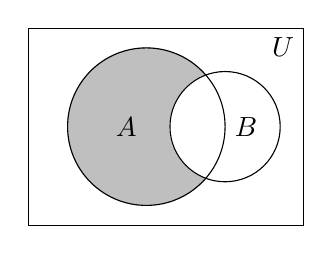
\begin{tikzpicture}
\draw (0,0) rectangle (3.5,2.5) node [below left] {$U$};
\filldraw [gray!50] (1.5,1.25) circle (1);
\filldraw [white] (2.5,1.25) circle (0.7);
\draw (1.5,1.25) circle (1) node [left] {$A$};
\draw (2.5,1.25) circle (0.7) node [right] {$B$};
\end{tikzpicture}\\
(2) 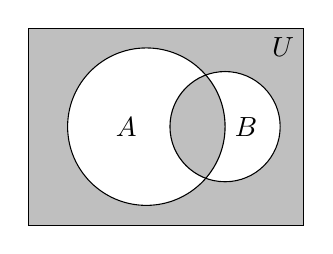
\begin{tikzpicture}
\filldraw [gray!50] (0,0) rectangle (3.5,2.5);
\draw (0,0) rectangle (3.5,2.5) node [below left] {$U$};
\filldraw [white] (1.5,1.25) circle (1);
\filldraw [white] (2.5,1.25) circle (0.7);
\begin{scope}
    \clip (1.5,1.25) circle (1);
    \clip (2.5,1.25) circle (0.7);
    \filldraw [gray!50] (0,0) rectangle (3.5,2.5);
\end{scope}
\draw (1.5,1.25) circle (1) node [left] {$A$};
\draw (2.5,1.25) circle (0.7) node [right] {$B$};
\end{tikzpicture}\\
(3) 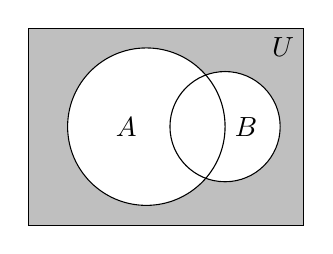
\begin{tikzpicture}
\filldraw [gray!50] (0,0) rectangle (3.5,2.5);
\draw (0,0) rectangle (3.5,2.5) node [below left] {$U$};
\filldraw [white] (1.5,1.25) circle (1);
\filldraw [white] (2.5,1.25) circle (0.7);
\draw (1.5,1.25) circle (1) node [left] {$A$};
\draw (2.5,1.25) circle (0.7) node [right] {$B$};
\end{tikzpicture}


关联目标:

暂未关联目标

答案: 暂无答案

解答或提示: 暂无解答与提示

使用记录:

暂无使用记录


出处: 2025届高一校本作业必修第一章
\item { (020067)}已知全集$U=A\cup B=\{x|0\le x\le 10, \ x\in \mathbf{N}\}$, $A\cap\overline B=\{1, 3, 5, 7\}$. 则集合$B=$\blank{50}.


关联目标:

暂未关联目标

答案: 暂无答案

解答或提示: 暂无解答与提示

使用记录:

暂无使用记录


出处: 2025届高一校本作业必修第一章
\item { (020068)}若全集$U=\{(x,y)|x\in\mathbf{R},\ y\in\mathbf{R}\}$, 集合$A=\{(x,y)|\dfrac yx=1\}$, 集合$B=\{(x,y)|y\neq x\}$, 则$\overline{A\cup B}= $\blank{50}.


关联目标:

暂未关联目标

答案: 暂无答案

解答或提示: 暂无解答与提示

使用记录:

暂无使用记录


出处: 2025届高一校本作业必修第一章
\item { (020069)}如图, 已知集合$U$为全集, 分别用集合$A$、$B$、$C$的运算式表示下列图中的阴影部分.
\begin{center}
    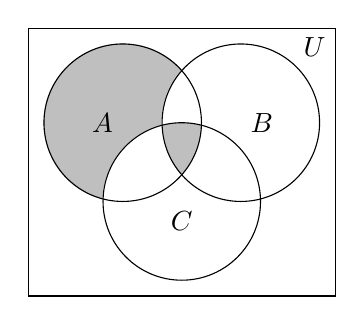
\begin{tikzpicture}
        \filldraw [gray!50] (0,0) circle (1);
        \filldraw [white] (1.5,0) circle (1);
        \filldraw [white] (0.75,-1) circle (1);
        \begin{scope}
            \clip (0,0) circle (1);
            \clip (1.5,0) circle (1);
            \clip (0.75,-1) circle (1);
            \filldraw [gray!50] (1.5,0) circle (1);
        \end{scope}
        \draw (0,0) circle (1) node [left] {$A$};
        \draw (1.5,0) circle (1) node [right] {$B$};
        \draw (0.75,-1) circle (1) node [below] {$C$};
        \draw (-1.2,-2.2) rectangle (2.7,1.2) node [below left] {$U$};
    \end{tikzpicture}
    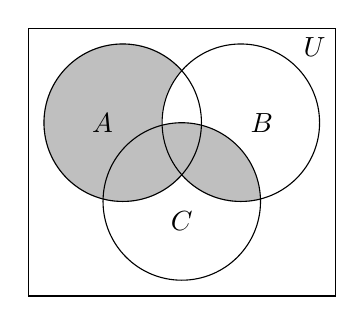
\begin{tikzpicture}
        \filldraw [gray!50] (0,0) circle (1);
        \filldraw [white] (1.5,0) circle (1);
        \begin{scope}
            \clip (0.75,-1) circle (1);
            \filldraw [gray!50] (1.5,0) circle (1);
        \end{scope}
        \draw (0,0) circle (1) node [left] {$A$};
        \draw (1.5,0) circle (1) node [right] {$B$};
        \draw (0.75,-1) circle (1) node [below] {$C$};
        \draw (-1.2,-2.2) rectangle (2.7,1.2) node [below left] {$U$};
    \end{tikzpicture}
\end{center}


关联目标:

暂未关联目标

答案: 暂无答案

解答或提示: 暂无解答与提示

使用记录:

暂无使用记录


出处: 2025届高一校本作业必修第一章
\item { (020070)}判断下列语句是否为命题, 并在相应的横线上填入``是''或``否''.\\
(1) 正方形和四边形;\blank{50};\\
(2) 正方形是四边形吗?\blank{50};\\
(3) $\pi>3$;\blank{50};\\
(4) 正方形好美!\blank{50};\\
(5) $2x>4$;\blank{50};\\
(6) $968$能被$11$整除;\blank{50}.


关联目标:

暂未关联目标

答案: 暂无答案

解答或提示: 暂无解答与提示

使用记录:

暂无使用记录


出处: 2025届高一校本作业必修第一章
\item { (020071)}判断下列命题的真假, 并在相应的括号内填入``真''或``假''.\\
(1) $2\sqrt 3>3\sqrt 2$或$1\le 1$;\blank{50};\\
(2) $2\sqrt 3>3\sqrt 2$且$1\le1$;\blank{50};\\
(3) 如果$a$、$b$都是奇数, 那么$ab$也是奇数;\blank{50};\\
(4) $\{1\}$是$\{0, 1, 2\}$的真子集;\blank{50};\\
(5) $1$是$\{0, 1, 2\}$的真子集;\blank{50};\\
(6) 若$x<-2$或$x>2$, 则$x^2>1$;\blank{50};\\
(7) 如果$|a|<2$, 那么$a<2$;\blank{50};\\
(8) 对任意实数$a,b$, 方程$(a+1)x+b=0$的解为$x=-\dfrac b{a+1}$;\blank{50};\\
(9) 若命题$\alpha$、$\beta$、$\gamma$满足$\alpha\Rightarrow \beta$, $\beta\Rightarrow \gamma$, $\gamma\Rightarrow \alpha$, 则$\alpha\Leftrightarrow \gamma$;\blank{50};\\
(10) 若关于$x$的方程$ax^2+bx+c=0$($a\ne 0$)的两实数根之积是正数, 则$ac>0$;\blank{50};\\
(11) 若某个整数不是偶数, 则这个数不能被$4$整除;\blank{50};\\
(12) 合数一定是偶数;\blank{50};\\
(13) 所有的偶数都是素数或合数;\blank{50};\\
(14) 所有的偶数都是素数或所有的偶数都是合数;\blank{50};\\
(15) 如果$A\subset B$, $B\supset C$, 那么$A=C$;\blank{50};\\
(16) 空集是任何集合的真子集;\blank{50};\\
(17) 若$x\in \mathbf{R}$, 则方程$x^2-x+1=0$不成立;\blank{50};\\
(18) 若$A\cap B\ne \varnothing$, $B\subset C$, 则$A\cap C\ne \varnothing$;\blank{50};\\
(19) 存在一个三角形, 它的任意两边的平方和小于第三边的平方;\blank{50};\\
(20) 对于任意一个三角形, 存在一组两边的平方和不等于第三边的平方;\blank{50}.


关联目标:

暂未关联目标

答案: 暂无答案

解答或提示: 暂无解答与提示

使用记录:

暂无使用记录


出处: 2025届高一校本作业必修第一章
\item { (020073)}已知命题``非空集合$M$的元素都是集合$P$的元素$''$是假命题, 给出下列命题: \textcircled{1} $M$中的元素都不是$P$的元素; \textcircled{2} $M$中有不属于$P$的元素; \textcircled{3} $M$中有$P$的元素; \textcircled{4} $M$中的元素不都是$P$的元素. 其中真命题有\blank{50}.


关联目标:

暂未关联目标

答案: 暂无答案

解答或提示: 暂无解答与提示

使用记录:

暂无使用记录


出处: 2025届高一校本作业必修第一章
\item { (020075)}已知$a$是常数, 命题$\alpha :-1<a<3$, $\beta$: 关于$x$的方程$x+a=0$($x\in \mathbf{R}$)没有正根, 若命题$\alpha$、$\beta$有且只有一个是真命题, 求实数$a$的取值范围.


关联目标:

暂未关联目标

答案: 暂无答案

解答或提示: 暂无解答与提示

使用记录:

暂无使用记录


出处: 2025届高一校本作业必修第一章
\item { (020084)}有限集合$S$中元素的个数记作$\mathrm{card}(S)$, 设$A,B$都是有限集合, 给出下列命题:\\
\textcircled{1} $A\cap B=\varnothing$的一个充要条件是$\mathrm{card}(A\cup B)=\mathrm{card}(A)+\mathrm{card}(B)$;\\
\textcircled{2} $A\subseteq B$的一个必要不充分条件是$\mathrm{card}(A)\le \mathrm{card}(B)$; \\
\textcircled{3} $A$不是$B$的子集的一个充分不必要条件是$\mathrm{card}(A)>\mathrm{card}(B)$;\\ 
\textcircled{4} $A=B$的一个充要条件是$\mathrm{card}(A)=\mathrm{card}(B)$.\\ 
其中真命题的个数是\bracket{20}.
\fourch{$0$}{$1$}{$2$}{$3$}


关联目标:

暂未关联目标

答案: 暂无答案

解答或提示: 暂无解答与提示

使用记录:

暂无使用记录


出处: 2025届高一校本作业必修第一章
\item { (020088)}在横线上写出下列命题的否定形式, 并判断命题真假, 在相应的位置中填入``真''或``假''.\\
(1) $\pi$是无理数; \blank{20}; \blank{150}; \blank{20};\\
(2) $2+1=4$;  \blank{20}; \blank{150}; \blank{20};\\
(3) 任何实数是正数或负数;  \blank{20}; \blank{150}; \blank{20};\\
(4) 任何实数是正数或任何实数是负数;  \blank{20}; \blank{150}; \blank{20};\\
(5) 对一切实数$x, x^3+1=0$;  \blank{20}; \blank{150}; \blank{20};\\
(6) 存在实数$x, x^3+1=0$;  \blank{20}; \blank{150}; \blank{20};\\
(7) 对于任意实数$k$, 关于$x$的方程$x^2+x+k=0$都有实数根;  \blank{20}; \blank{250}; \blank{20};\\
(8) 任何三角形中至多有一个钝角;  \blank{20}; \blank{150}; \blank{20};\\
(9) 若$a>1$, $b>1$, 则$ab>1$;  \blank{20}; \blank{150}; \blank{20};\\
(10) 能被$2$整除的整数是质数;  \blank{20}; \blank{150}; \blank{20}.\\


关联目标:

暂未关联目标

答案: 暂无答案

解答或提示: 暂无解答与提示

使用记录:

暂无使用记录


出处: 2025届高一校本作业必修第一章
\item { (020089)}写出下列命题的否定形式.\\
(1) 在平面上, 过定点$P$有且只有一条直线垂直于给定直线$l$;\\
(2) 任意两个有理数之间存在一个无理数;\\
(3) 存在实数$a$, 使得关于$x$的不等式$x^2+(a-2)x+a-1\ge 0$至少有一个正数解;\\
(4) 存在实数$a$, 使得关于$x$的不等式$x^2+(a-2)x+a-1\ge 0$恒成立;\\
(5) 存在实数$a$, 使得关于$x$的不等式$x^2+(a-2)x+a-1\ge 0$有解.


关联目标:

暂未关联目标

答案: 暂无答案

解答或提示: 暂无解答与提示

使用记录:

暂无使用记录


出处: 2025届高一校本作业必修第一章
\end{enumerate}



\end{document}